\documentclass%
%[handout]
{beamer}
% % % % % % % %
%IMPORTANT
%compiles with
%pdflatex -shell-escape
%IMPORTANT
% % % % % % % %
\usepackage{ifthen}
\usepackage{amsmath}
\usepackage{amssymb}
\usepackage{cancel}
\usepackage{comment}
\usepackage{multirow}
\usepackage{psfrag}
\usepackage{rotating}
\usepackage{fp}
\usepackage{calc}
\usepackage{bm}
\usepackage[all,cmtip]{xy}
\RequirePackage{xstring}

%%%%%%%%%%%%%%%%%%%%%%%%%%%%%%%%%%%%%%%%%%
%
% List of commands in this document
%
%
% \logdiffbaseandexp
% \logdifftwouponedown
% \productrulefofx
% \quotientruley
% \limitradical  (broken)
% \limitsub
% \chainruley
% \chainrulefofx
% \chainruleStyleOne
% \chainruleStyleTwo
% \chainruleStyleThree
% \infinitelimit
% \limitfactor
% \newtonsmethod
% \constantmultiple
% \chainruletwice
% \youWillNotBeTested
% \optionalDisplay  %Dummy command needed for compatibility with Calculus notes.
% \Arcsin
% \Arccos
% \Arctan
% \Arccot
% \diff
%%%%%%%%%%%%%%%%%%%%%%%%%%%%%%%%%%%%%%%%%%

\newcommand{\diff}{{\normalfont \text{d}}}
\newtheorem{question}{Question}
\newtheorem{observation}{Observation}
\newtheorem{proposition}{Proposition}
\newtheorem{remark}{Remark}
\newcommand{\youWillNotBeTested}{\begin{frame}You will not be tested on the material in the following slide.\end{frame}}
\DeclareMathOperator{\Vol}{Vol}

\DeclareMathOperator{\Arcsin}{\sin^{-1}}
\DeclareMathOperator{\Arccos}{\cos^{-1}}
\DeclareMathOperator{\Arctan}{\tan^{-1}}
\DeclareMathOperator{\Arccot}{{\cot^{-1}}}
\DeclareMathOperator{\Arcsec}{{\sec^{-1}}}
\DeclareMathOperator{\Arccsc}{{\csc^{-1}}}
\DeclareMathOperator{\maclaurin}{{\normalfont{Mc}}}
\newcommand{\taylor}{{\normalfont{T}}}

\newcommand{\optionalDisplay}[1]{#1}
\renewcommand{\Im}{\mathrm{Im}}
\renewcommand{\Re}{\mathrm{Re}}

%\DeclareMathOperator{\Re}{Re}
%\DeclareMathOperator{\Im}{Im}
\newcommand{\fcv}[1]{{\bf #1}} %this command stands for freecalc Vector
\DeclareMathOperator{\curl}{\fcv{curl}}
\DeclareMathOperator{\divg}{div}
\DeclareMathOperator{\proj}{\fcv{proj}}
\DeclareMathOperator{\orth}{\fcv{orth}}
\DeclareMathOperator{\grad}{\fcv{grad}}
\newcommand{\RR}{{\mathbb{R}}}
\newcommand{\cR}{{\mathcal{R}}}
\newcommand{\cD}{{\mathcal{D}}}
\newcommand{\cP}{{\mathcal{P}}}
\newcommand{\fcUncoverAlert}[2]{\uncover<#1->{\alert<#1>{#2}}}
\newcommand{\alertNoH}[2]{\alert<handout:0|#1>{#2}}
\newcommand{\fcAnswerNoH}[2]{
\FPeval{\fcResult}{clip(#1-1)}
\uncover<handout:0|\fcResult>{\alert<handout:0|\fcResult>{\textbf{?} }} \uncover<handout:0| #1->{\alert<handout:0|#1>{\!\!\!#2}}
}
\newcommand{\fcAnswer}[2]{
\FPeval{\fcResult}{clip(#1-1)}
\uncover<handout:0|\fcResult>{\alertNoH{\fcResult}{\textbf{?} }} \uncover<#1->{\alertNoH{#1}{\!\!\!#2}}
}
\newcommand{\fcAnswerUncover}[3]{
\FPeval{\fcResult}{clip(#2-1)}
\uncover<handout:0|#1-\fcResult>{\alertNoH{\fcResult}{\textbf{?}}} \uncover<#2->{\alertNoH{#2}{\!\!\!#3}}
}
\newcommand{\fcAnswerUncoverNoH}[3]{
\FPeval{\fcResult}{clip(#2-1)}
\uncover<handout:0|#1-\fcResult>{\alertNoH{\fcResult}{\textbf{?}}} \uncover<handout:0|#2->{\alertNoH{#2}{\!\!\!#3}}
}

\newcommand{\fcQuestion}[2]{%
\FPeval{\fcResult}{clip(#1+1)}%
\uncover<#1->{\alertNoH{ #1,\fcResult}{#2}}%
}
\newcommand{\fcEvalToInt}[1]{\FPeval{\fcResult}{clip(#1)}\fcResult}
\newcommand{\refBad}[3]{%
\ifthenelse{\equal{#1}{??}}%
{#2}%
{#3}%
}%example usage: \refBad{\ref{eqMacLaurinDef}}{their definition}{their definition (Definition \ref{eqMacLaurinDef})}
\newcommand{\fcCancel}[2]{
\FPeval{\fcResult}{clip(#1-1)}
\only<handout:0|-\fcResult>{#2} \only<#1->{\alertNoH{#1}{\cancel{\alertNoH{0}{#2}}}}
\vphantom{\cancel{#2}}
}
%<-WARNING: the superflous-looking \alertNoH{0} is needed:
% for some unknown to me reason it causes LaTeX to add the correct amount of spacing.

%code blocks regular expression that replaces all strings of the form \alert<handout:0| a> by \alertNoH{a}:
%Find:
%\\alert<[^|^0]*0|\([^>]*\)>
%Replace:
%\\alertNoH{\1}
%code blocks regular expression that replaces all strings of the form \alert<a> but not containing | by \alertNoH{a}:
%Find:
%\\alert<\([^|^>]*\)>
%Replace:
%\\alertNoH{\1}


\newcommand{\fcLicense}{
\begin{frame}
\frametitle{License to use and redistribute}
These lecture slides and their $\LaTeX${} source code are licensed to you under the Creative Commons license CC BY 3.0. You are free
\begin{itemize}
\item to Share - to copy, distribute and transmit the work,
\item to Remix - to adapt, change, etc., the work,
\item to make commercial use of the work,
\end{itemize}
as long as you reasonably acknowledge the original project (a notice of use freecalc is sufficient).
\begin{itemize}
\item Latest version of the .tex sources of the slides: \url{https://sourceforge.net/p/freecalculus/code/HEAD/tree/}
\item Should the link be outdated/moved, search for  ``freecalc project''.
\item Creative Commons license CC BY 3.0:
\url{https://creativecommons.org/licenses/by/3.0/us/}
and the links therein.
\end{itemize}
\end{frame}
}


\newcommand{\onlyNoH}[2]{\only<handout:0|#1>{#2}}
%
%  An example of logarithmic differentiation of a function with a
%  variable base and exponent.
%  #1 is the base.
%  #2 is the exponent.
%  #3 is the derivative of the natural logarithm of the base.
%  #4 is the derivative of the exponent.
%  #5 is (base)(exponent)' + (exponent)(base)' after simplification.
%
\newcommand{\logdiffbaseandexp}[5]{
\begin{example}[Variable base and exponent]
\abovedisplayskip=0pt
\belowdisplayskip=0pt
\abovedisplayshortskip=0pt
\belowdisplayshortskip=0pt
\begin{align*}
\text{Differentiate}\quad \alertNoH{ 13}{y} %
 & \alertNoH{ 13}{=} %
\alertNoH{ 13}{%
#1^{#2}%
}.%
\uncover<2->{%
\intertext{
Take logarithms of both sides:%
}
}%
\uncover<2->{%
\ln y
}%
 & \uncover<2->{ = } %
\uncover<2->{%
\ln #1^{\alertNoH{ 3}{#2}}%
}\\%
\uncover<3->{%
\alertNoH{ 4-5}{\ln y}%
}%
 & \uncover<3->{ = } %
\uncover<3->{%
\alertNoH{ 6-7}{%
\alertNoH{ 3}{#2} \ln #1%
}.}%
\uncover<4->{%
\intertext{
Differentiate implicitly with respect to $x$:%
}%
}%
\fcAnswer{5}{\frac{1}{y} y'}%
 & \uncover<4->{ = } %
\fcAnswerUncover{4}{7}{%
\left( #2 \right) \alertNoH{ 8-9}{\frac{\diff}{\diff x} \left( \ln #1 \right)} + \left( \ln #1 \right)\alertNoH{ 10-11}{\frac{\diff}{\diff x}\left( #2 \right)} %
}\\%
\uncover<8->{%
\frac{1}{\alertNoH{12}{y}} y'%
}%
 & \uncover<8->{ = } %
\uncover<8->{%
( #2 ) \alertNoH{8-9}{\left( \fcAnswerUncover{8}{9}{ #3 }\right)} + \left( \ln #1 \right) \alertNoH{ 10-11}{ \left( \fcAnswerUncover{8}{11}{ #4 } \right) }
}\\%
\uncover<12->{%
y'%
}%
 & \uncover<12->{ = } %
\uncover<12->{%
\alertNoH{ 12-13}{y} \left( #5 \right)%
}\\%
 & \uncover<13->{ = } %
\uncover<13->{%
\alertNoH{ 13}{#1^{#2}} \left( #5 \right).%
}%
\end{align*}
\end{example}
}


%
%  An example of logarithmic differentiation of a function.
%  It looks as follows:
%
%  Differentiate y = (#1 #2)/#3.
%  Take logarithms of both sides:
%  ln y = ln((#1 #2)/#3)
%  ln y = ln#1 + ln#2 - ln#3
%  ln y = #4 + #5 - #6
%  Differentiate implicitly with respect to x:
%  (1/y)y' = #7 + #8 - #9
%  y' = y(#7 + #8 - #9)
%  y' = ((#1 #2)/#3)(#7 + #8 - #9)
%
\newcommand{\logdifftwouponedown}[9]{
\begin{example}[Logarithmic Differentiation%
]
\abovedisplayskip=0pt
\belowdisplayskip=0pt
\abovedisplayshortskip=0pt
\belowdisplayshortskip=0pt
\begin{align*}
\text{Differentiate}\quad \alertNoH{ 18}{y} %
 & \alertNoH{ 18}{=} %
\alertNoH{ 18}{%
\frac{#1 #2}{#3}%
}.%
\uncover<2->{%
\intertext{
Take logarithms of both sides:%
}
}%
\uncover<2->{%
\ln y
}%
 & \uncover<2->{ = } %
\uncover<2->{%
\ln \frac{\alertNoH{ 3-4}{#1}\alertNoH{ 5-6}{#2}}{\alertNoH{ 7-8}{#3}}%
}\\%
\uncover<2->{%
\ln y
}%
 & \uncover<2->{ = } %
\uncover<2->{%
\ln \alertNoH{ 3-4}{#1} + \ln \alertNoH{ 5-6}{#2} -  \ln \alertNoH{ 7-8}{#3}%
}\\%
\uncover<3->{%
\alertNoH{ 9-10}{\ln y}%
}%
 & \uncover<3->{ = } %
\uncover<3->{%
\alertNoH{ 3-4,11-12}{%
\left( \uncover<4->{#4}\right) %
}%
\alertNoH{ 5-6}{%
\uncover<6->{+} \alertNoH{ 13-14}{\left( \uncover<6->{#5}\right)} %
}%
\alertNoH{ 7-8}{%
\uncover<8->{-} \alertNoH{ 15-16}{\left( \uncover<8->{#6}\right)} %
}%
}%
\uncover<9->{%
\intertext{
Differentiate implicitly with respect to $x$:%
}%
}%
\uncover<10->{%
\alertNoH{ 10}{\frac{1}{\alertNoH{ 17}{y}} y'}%
}%
 & \uncover<9->{ = } %
\uncover<9->{%
\alertNoH{ 11-12}{\left( \uncover<12->{#7} \right)} + %
\alertNoH{ 13-14}{\left( \uncover<14->{#8} \right)} - %
\alertNoH{ 15-16}{\left( \uncover<16->{#9} \right)} %
}\\%
\uncover<17->{%
y'%
}%
 & \uncover<17->{ = } %
\uncover<17->{%
\alertNoH{ 17-18}{y} \left( #7 + #8 - #9 \right)%
}\\%
 & \uncover<18->{ = } %
\uncover<18->{%
\alertNoH{ 18}{\frac{#1 #2}{#3}} \left( #7 + #8 - #9 \right)%
}%
\end{align*}
\end{example}
}


%
%  An example of a derivative with the Product Rule, using the symbol f(x).
%  It looks as follows:
%
%  Differentiate f(x) = #1 #2.
%  Product Rule: f'(x) = (#1)(d/dx)(#2) + (#2)(d/dx)(#1)
%   = (#1)(#4) + (#2)(#3)
%   = #5.
%
%  #6 appears in the subtitle of the example.
%
\newcommand{\productrulefofx}[6]{%
\begin{example}[Product Rule%
\ifthenelse{\equal{#6}{0}}%
{}%
{, #6}%
]%
\abovedisplayskip=0pt
\belowdisplayskip=0pt
\abovedisplayshortskip=0pt
\belowdisplayshortskip=0pt
\begin{align*}
\text{Differentiate}\quad f(x) & = \alertNoH{2}{ #1}\alertNoH{3}{ #2.}\\%
\uncover<2->{%
\text{Product Rule:}\quad f'(x)%
}%
& \uncover<2->{%
 =  \alertNoH{ 6-7}{\frac{\diff}{\diff x}\left( \alertNoH{2}{#1} \right)}\left( \alertNoH{3}{#2} \right)+\left( \alertNoH{2}{#1} \right) \alertNoH{ 4-5}{\frac{\diff}{\diff x}\left( \alertNoH{3}{#2} \right)} %
}\\%
& \uncover<4->{%
 = \alertNoH{ 6-7}{\left( \fcAnswerUncover{4}{7}{#3} \right)}\left( #2 \right)+ \left( #1 \right) \alertNoH{ 4-5}{\left(\fcAnswer{5}{ #4 }\right)}  %
}\\%
& \uncover<8->{%
 = #5.%
}%
\end{align*}
\end{example}
}


%
%  An example of a derivative with the Constant Multiple Rule.
%  It looks as follows:
%
%  Find the derivative of #1 = #2.
%   #1 = (#3)(#4).
%   d#1/dx = (d/dx)((#3)(#4))
% Constant Multiple Rule: = (#3)(d/dx)(#4)
%   = (#3)(#5)
%   = #6.
%
%  #7 appears in the subtitle of the example.
%
\newcommand{\constantmultiple}[7]{%
\begin{example}[Constant Multiple Rule%
\ifthenelse{\equal{#7}{0}}%
{}%
{, #7}%
]%
\abovedisplayskip=0pt
\belowdisplayskip=0pt
\abovedisplayshortskip=0pt
\belowdisplayshortskip=0pt
\begin{align*}
\text{Find the derivative of}\quad #1 & = #2.\\%
\uncover<2->{%
#1 %
}%
& \uncover<2->{%
 = \left( #3\right)\left( #4\right).
}\\%
\uncover<3->{%
\frac{\diff #1}{\diff x} %
}%
& \uncover<3->{%
 = \frac{\diff}{\diff x}\left[ \alertNoH{ 4}{\left( #3\right)}\left( #4\right)\right]
}\\%
\uncover<4->{%
\text{Constant Multiple Rule:}\quad %
}%
& \uncover<4->{%
 =  \alertNoH{ 4}{\left( #3\right)}\alertNoH{ 5-6}{\frac{\diff}{\diff x}\left( #4\right)}
}\\%
& \uncover<5->{%
 =  \left( #3\right)\alertNoH{ 5-6}{\left( \fcAnswer{6}{#5}\right)}
}\\%
& \uncover<7->{%
 =  #6.
}%
\end{align*}
\end{example}
}


%
%  An example of a derivative with the Quotient Rule, using the symbol y.
%  It looks as follows:
%
%  Differentiate y = #1 / #2.
%  Quotient Rule: dy/dx = ((#2)(d/dx)(#1)-(#1)(d/dx)(#2))/(#2)^2
%   = ((#2)(#3)-(#1)(#4))/(#2)^2
%   = #5
%   = #6.
%
%  #7 appears in the subtitle of the example.
%
\newcommand{\quotientruley}[7]{%
\begin{example}[Quotient Rule%
\ifthenelse{\equal{#7}{0}}%
{}%
{, #7}%
]%
\abovedisplayskip=0pt
\belowdisplayskip=0pt
\abovedisplayshortskip=0pt
\belowdisplayshortskip=0pt
\begin{align*}
\text{Differentiate}\quad y & = \frac{\alertNoH{2}{ #1}}{\alertNoH{3}{#2}}.%
\uncover<2->{%
\intertext{Quotient Rule:}%
}%
%&\\%
\uncover<2->{%
\frac{\diff y}{\diff x}%
}%
& \uncover<2->{%
 = \frac%
{ \alertNoH{ 4-5}{\frac{\diff}{\diff x}\left( \alertNoH{2}{ #1} \right)}\left( \alertNoH{3}{#2} \right) - \left( \alertNoH{2}{#1} \right) \alertNoH{ 6-7}{\frac{\diff}{\diff x}\left( \alertNoH{3}{#2} \right)}}%
{\left( \alertNoH{3}{#2}\right)^2}%
}\\%
& \uncover<4->{%
 = \frac%
{\alertNoH{ 4-5}{\left(\fcAnswer{5}{ #3 }\right)}\left( #2 \right)  - \left( #1 \right) \alertNoH{ 6-7}{\left( \fcAnswerUncover{4}{7}{#4} \right)}}%
{\left( #2\right)^2}%
}\\%
& \uncover<8->{%
 = #5%
}\\%
& \uncover<9->{%
 = #6.%
}%
\end{align*}
\end{example}
}

%
%  An example of an indefinite integral with the Substitution Rule.
%  It looks as follows:
%
%  Find \int (#1, with nothing substituted for UU and VV).
%  Let u = #2
%  Then du = #3.
%  Therefore #4 = #5.
%  Substitute: \int (#1, with the alert command for u and du
%          substituted for UU and VV respectively)
%  = \int (#6, with the alert command for u and du substituted for UU and VV)
%  = (#7, with u substituted for UU) + C
%  = (#8, with #2 substituted for UU) + C
%
%  #9 appears in the subtitle of the example.
%
\newcommand{\subrule}[9]{%
\begin{example}[Substitution Rule%
\ifthenelse{\equal{#9}{0}}%
{}%
{, #9}%
]%
\abovedisplayskip=0pt
\belowdisplayskip=0pt
\abovedisplayshortskip=0pt
\belowdisplayshortskip=0pt
\begin{align*}
\text{Find}\quad \int %
 \noexpandarg\exploregroups\StrSubstitute{\StrSubstitute{#1}{UU}{3}}{VV}{6-7}\noexploregroups\expandarg. & \\%
\uncover<2->{%
\text{Let}\quad\alertNoH{ 2-3,8,13}{u}%
}%
& \uncover<2->{%
\alertNoH{ 2-3,8,13}{ = \uncover<3->{#2.}}%
}\\%
\uncover<4->{%
\text{Then}\quad \alertNoH{ 4-5}{\diff u}%
}%
& \uncover<4->{%
\alertNoH{ 4-5}{ = \uncover<5->{#3}}%
}\\%
\uncover<6->{%
\alertNoH{ 6-7,9}{#4}%
}%
& \uncover<6->{%
\alertNoH{ 6-7,9}{ = \uncover<7->{#5.}}%
}\\%
\uncover<8->{%
\text{Substitute:}\quad \int%
 \noexpandarg\exploregroups\StrSubstitute{\StrSubstitute{#1}{UU}{8}}{VV}{9}\noexploregroups\expandarg}%
& \uncover<8->{= \alertNoH{ 10-11}{\int\noexpandarg\exploregroups\StrSubstitute{\StrSubstitute{#6}{UU}{8}}{VV}{9}\noexploregroups\expandarg %
}}\\%
& \uncover<10->{\alertNoH{ 10-11}{%
 = \uncover<11->{\noexpandarg\exploregroups \StrSubstitute{#7}{UU}{\alertNoH{ 13}{u}}\noexploregroups\expandarg} \uncover<12->{\alertNoH{ 12}{+C}}%
}}\\%
& \uncover<13->{%
 = \noexpandarg\exploregroups \StrSubstitute{#8}{UU}{\alertNoH{ 13}{#2}}\noexploregroups\expandarg +C.%
}%
\end{align*}
\end{example}
}

%
%  An example of a definite integral with the Substitution Rule.
%  There are nine arguments to the function.  The ninth is a string of four
%  groups of the form {AA}{BB}{CC}{DD} where AA is the lower limit of
%  integration, BB is the upper limit of integration, CC is the lower limit
%  of integration with respect to u, and DD is the upper limit of integration
%  with respect to u.
%  It looks as follows:
%
%  Find \int_{AA}^{BB} (#1, with nothing substituted for UU and VV).
%  Let u = #2
%  Then du = #3.
%  #4 = #5.
%  When x = AA, u = CC.
%  When x = BB, u = DD.
%  Substitute: \int_{AA}^{BB} (#1, with the alert command for u and du
%          substituted for UU and VV respectively)
%  = \int_{CC}^{DD} (#6, with the alert command for u and du substituted for UU and VV)
%  = [#7, with u substituted for UU]_{CC}^{DD}
%  = #8.
%
%
\newcommand{\subruledefbounds}[9]{%
\begin{example}[Substitution Rule, Definite Integral%
]%
\abovedisplayskip=0pt
\belowdisplayskip=0pt
\abovedisplayshortskip=0pt
\belowdisplayshortskip=0pt
\begin{align*}
\text{Find}\quad \int%
_{\StrMid{#9}{1}{1}}%
^{\StrMid{#9}{2}{2}} %
 \noexpandarg\exploregroups\StrSubstitute{\StrSubstitute{#1}{UU}{3}}{VV}{6-7}\noexploregroups\expandarg. & \\%
\uncover<2->{%
\text{Let}\quad\alertNoH{ 2-3,8-12}{u}%
}%
& \uncover<2->{%
\alertNoH{ 2-3,8-12}{ = \uncover<3->{#2.}}%
}\\%
\uncover<4->{%
\text{Then}\quad \alertNoH{ 4-5}{\diff u}%
}%
& \uncover<4->{%
\alertNoH{ 4-5}{ = \uncover<5->{#3}}%
}\\%
\uncover<6->{%
\alertNoH{ 6-7,13}{#4}%
}%
& \uncover<6->{%
\alertNoH{ 6-7,13}{ = \uncover<7->{#5.}}%
}\\%
\uncover<8->{%
\alertNoH{ 8-9,14}{\text{When } x = \StrMid{#9}{1}{1}, \quad u }%
}%
& \uncover<8->{%
\alertNoH{ 8-9,14}{ = \uncover<9->{\StrMid{#9}{3}{3}.}}%
}\\%
\uncover<10->{%
\alertNoH{ 10-11,15}{\text{When } x = \StrMid{#9}{2}{2}, \quad u }%
}%
& \uncover<10->{%
\alertNoH{ 10-11,15}{ = \uncover<11->{\StrMid{#9}{4}{4}.}}%
}\\%
\uncover<12->{%
\text{Substitute:}\quad \int%
_{\alertNoH{ 14}{\StrMid{#9}{1}{1}}}%
^{\alertNoH{ 15}{\StrMid{#9}{2}{2}}} %
 \noexpandarg\exploregroups\StrSubstitute{\StrSubstitute{#1}{UU}{12}}{VV}{13}\noexploregroups\expandarg}%
& \uncover<12->{= \alertNoH{ 16-17}{{\int}%
_{\uncover<14->{\alertNoH{ 14}{
\StrMid{#9}{3}{3}}}}%
^{\uncover<15->{
\alertNoH{ 15}{
\StrMid{#9}{4}{4}}}} %
\noexpandarg\exploregroups\StrSubstitute{\StrSubstitute{#6}{UU}{12}}{VV}{13}\noexploregroups\expandarg %
}}\\%
& \uncover<16->{\alertNoH{ 16-17}{%
 = {\left[ \uncover<17->{%
\noexpandarg\exploregroups\StrSubstitute{#7}{UU}{u}\noexploregroups\expandarg %
}\right]}_{\StrMid{#9}{3}{3}}^{\StrMid{#9}{4}{4}}%
}}\\%
& \uncover<18->{%
 = #8.
}%
\end{align*}
\end{example}
}


%
%  An example of a definite integral with the Substitution Rule.
%  There are nine arguments to the function.  The ninth is a string of two
%  groups of the form {AA}{BB} where AA is the lower limit of
%  integration and BB is the upper limit of integration.
%  It looks as follows:
%
%  Find \int_{AA}^{BB} (#1, with nothing substituted for UU and VV).
%  Let u = #2
%  Then du = #3.
%  #4 = #5.
%  Substitute: \int (#1, with the alert command for u and du
%          substituted for UU and VV respectively)
%  = \int (#6, with the alert command for u and du substituted for UU and VV)
%  = #7, with u substituted for UU
%  = #8.
%  Therefore int_{AA}^{BB} (#1, with nothing substituted for UU and VV)
%      = [#8]_{AA}^{BB}
%  = #9.
%
%
\newcommand{\subruledefvar}[9]{%
\begin{example}[Substitution Rule, Definite Integral%
]%
\abovedisplayskip=0pt
\belowdisplayskip=0pt
\abovedisplayshortskip=0pt
\belowdisplayshortskip=0pt
\begin{align*}
\text{Find}\quad \int%
_{\StrMid{#9}{1}{1}}%
^{\StrMid{#9}{2}{2}} %
 \noexpandarg\exploregroups\StrSubstitute{\StrSubstitute{#1}{UU}{3}}{VV}{6-7}\noexploregroups\expandarg. & \\%
\uncover<2->{%
\text{Let}\quad\alertNoH{ 2-3,8,12}{u}%
}%
& \uncover<2->{%
\alertNoH{ 2-3,8,12}{ = \uncover<3->{#2.}}%
}\\%
\uncover<4->{%
\text{Then}\quad \alertNoH{ 4-5}{\diff u}%
}%
& \uncover<4->{%
\alertNoH{ 4-5}{ = \uncover<5->{#3}}%
}\\%
\uncover<6->{%
\alertNoH{ 6-7,9}{#4}%
}%
& \uncover<6->{%
\alertNoH{ 6-7,9}{ = \uncover<7->{#5.}}%
}\\%
\uncover<8->{%
\text{Substitute:}\quad \int%
 \noexpandarg\exploregroups\StrSubstitute{\StrSubstitute{#1}{UU}{8}}{VV}{9}\noexploregroups\expandarg}%
& \uncover<8->{= \alertNoH{ 10-11}{{\int}%
\noexpandarg\exploregroups\StrSubstitute{\StrSubstitute{#6}{UU}{8}}{VV}{9}\noexploregroups\expandarg %
}}\\%
& \uncover<10->{%
 \alertNoH{ 10-11}{ = \uncover<11->{%
\noexpandarg\exploregroups{\StrSubstitute{#7}{UU}{\alertNoH{ 12}{u}}}\noexploregroups\expandarg%
}}%
  \uncover<12->{%
 = \noexpandarg\exploregroups{\StrSubstitute{#7}{UU}{\alertNoH{ 12}{#2}}}\noexploregroups\expandarg.%
}%
}\\%
\uncover<13->{%
\text{Therefore}\quad \int%
_{\StrMid{#9}{1}{1}}%
^{\StrMid{#9}{2}{2}} %
 \noexpandarg\exploregroups\StrSubstitute{\StrSubstitute{#1}{UU}{0}}{VV}{0}\noexploregroups\expandarg}%
& \uncover<13->{%
 = \left[%
 \noexpandarg\exploregroups{\StrSubstitute{#7}{UU}{#2}}\noexploregroups\expandarg%
\right]%
_{\StrMid{#9}{1}{1}}%
^{\StrMid{#9}{2}{2}} %
}\\%
& \uncover<14->{%
 = #8.
}%
\end{align*}
\end{example}
}

%
%  An example of a derivative with the Chain Rule, using the symbol y.
%  It looks as follows:
%
%  Differentiate y = #1.
%  Let u = #2
%  Then y = #3
%  Chain Rule: dy/dx = (dy/du)(du/dx)
%  = (#4, with u substituted for UU)(#5)
%  = #6, with #2 substituted for UU
%
%  #7 appears in the subtitle of the example.
%
\newcommand{\chainruley}[7]{%
\begin{example}[Chain Rule%
\ifthenelse{\equal{#7}{0}}%
{}%
{, #7}%
]%
\abovedisplayskip=0pt
\belowdisplayskip=0pt
\abovedisplayshortskip=0pt
\belowdisplayshortskip=0pt
\begin{align*}
\text{Differentiate}\quad y & = #1.\\%
\uncover<2->{%
\text{Let}\quad\alertNoH{ 2-3,8-10}{u}%
}%
& \uncover<2->{%
\alertNoH{ 2-3,8-10}{ = \uncover<3-| handout:0>{#2.}}%
}\\%
\uncover<4->{%
\text{Then}\quad \alertNoH{ 6-7}{y}%
}%
& \uncover<4->{%
\alertNoH{ 6-7}{ = \uncover<4-| handout:0>{#3.}}%
}\\%
\uncover<5->{%
\text{Chain Rule:}\quad%
\frac{\diff y}{\diff x}%
}%
& \uncover<5->{%
 = \alertNoH{ 6-7}{\frac{\diff y}{\diff u}}%
\alertNoH{ 8-9}{\frac{\diff u}{\diff x}}%
}\\%
& \uncover<6->{%
 = \alertNoH{ 6-7}{\left( \uncover<7-| handout:0>{\noexpandarg\exploregroups\StrSubstitute{#4}{UU}{\alertNoH{ 10}{u}}\noexploregroups\expandarg}\right)}%
\alertNoH{ 8-9}{\left( \uncover<9-| handout:0>{#5}\right)}%
}\\%
& \uncover<10->{ = } \uncover<10-| handout:0>{%
 \noexpandarg\exploregroups \StrSubstitute{#6}{UU}{\alertNoH{ 10}{#2}}.\noexploregroups\expandarg%
}%
\end{align*}
\end{example}
}





%
%  An example of a derivative with the Chain Rule, using the symbol f(x).
%  It looks as follows:
%
%  Differentiate f(x) = #1.
%  Let h(x) = #2
%  Let g(x) = #3
%  Then f(x) = g(h(x))
%  f'(x) = g'(h(x))h'(x)
%  = (#4, with h(x) substituted for UU)(#5)
%  = #6, with #2 substituted for UU
%
%  #7 appears in the subtitle of the example.
%
\newcommand{\chainrulefofx}[7]{%
\begin{example}[Chain Rule%
\ifthenelse{\equal{#7}{0}}%
{}%
{, #7}%
]%
\abovedisplayskip=0pt
\belowdisplayskip=0pt
\abovedisplayshortskip=0pt
\belowdisplayshortskip=0pt
\begin{align*}
\text{Differentiate}\quad f(x) & = #1.\\%
\uncover<2->{%
\text{Let}\quad\alertNoH{ 2-3,9-11}{h(x)}%
}%
& \uncover<2->{%
\alertNoH{ 2-3,9-11}{ = \fcAnswerNoH{3}{#2.}}%
}\\%
\uncover<2->{%
\text{Let}\quad\alertNoH{ 4-5,7-8}{g(x)}%
}%
& \uncover<2->{%
\alertNoH{ 4-5,7-8}{ = \fcAnswerUncover{2}{5}{#3.}}%
}\\%
\uncover<2-| handout:0>{%
\text{Then}\quad f(x)%
}%
& \uncover<2-| handout:0>{%
 = g(h(x)).%
}\\%
\uncover<6-| handout:0>{%
\text{Chain Rule:}\quad%
f'(x)%
}%
& \uncover<6-| handout:0>{%
 = \alertNoH{ 7-8}{g'(h(x))}%
\alertNoH{ 9-10}{h'(x)}%
}\\%
& \uncover<7-| handout:0>{%
=}\uncover<7-| handout:0>{\alertNoH{ 7-8}{\left( \fcAnswerNoH{8}{\noexpandarg\exploregroups\StrSubstitute{#4}{UU}{\alertNoH{ 11}{h(x)}}\noexploregroups\expandarg}\right)}%
\alertNoH{ 9-10}{\left( \fcAnswerUncoverNoH{7}{10}{#5}\right)}%
}\\%
& \uncover<11-| handout:0>{=} \uncover<11-| handout:0>{%
 \noexpandarg \exploregroups \StrSubstitute{#6}{UU}{\alertNoH{ 11}{#2}}.\noexploregroups \expandarg%
}%
\end{align*}
\end{example}
}

%
%  Similar to chainrulefofx but in different style.
%  It looks as follows:
%
%  Recall the chain rule (...).
%******************************
%  Differentiate f(x) = #1.
%  h(x) = #2
%  Let g(u) = #3
%  Then g'(u)=#4
%  Then f(x) = g(u)
%  f'(x) = g'(u)h'(x)
%  = (#4, with h(x) substituted for UU)(#5)
%  = #6, with #2 substituted for UU
%
%  #7 appears in the subtitle of the example.
%
\newcommand{\chainruleStyleOne}[7]{%
{\renewcommand{\arraystretch}{1.2}
$
\begin{array}{rclll}
\alertNoH{1-}{\left(g(h(x))\right)'}&\alertNoH{1-}{=}&\alertNoH{1-}{g'(h(x))\cdot  h'(x)}&& \text{(notation 1)} {~~~~~~~~~~~~~~~~~~~~~~~~~~~~~~~~~~~~} \\
(g(u))'&\alertNoH{0}{=}&g'(u) u'&\text{where } u=h(x)& \text{(notation 2)}\\
\displaystyle\frac{\diff y}{\diff x} &\alertNoH{0}{=}& \displaystyle\frac{\diff y}{\diff u}  \frac{\diff u}{\diff x} &\text{where } y=g(u)& \text{(notation 3)}\quad.\\
\end{array}
$
}
\begin{example}[Chain Rule, Notation 1%
\ifthenelse{\equal{#7}{0}}%
{}%
{, #7}%
]%
\[
\begin{array}{rrcl}
\text{Differentiate } & f(x) & =& #1.\\%
\uncover<2->{%
\text{Let}&\alertNoH{2-3,9-11}{h(x)}%
}%
&\uncover<2-| handout:0>{\alertNoH{2-3, 9-11}{ = }} &\displaystyle \uncover<2-| handout:0>{%
\alertNoH{2-3,9-11}{ \fcAnswerNoH{3}{#2.}}%
}\\%
\uncover<2->{%
\text{Let}&\alertNoH{4-5,7-8}{g(u)}%
}
&\uncover<2->{\alertNoH{4-5,7-8}{=}}&\displaystyle
\uncover<2->{\alertNoH{4-5,7-8}{ \fcAnswerUncover{2}{5}{\uncover<5-| handout:0>{#3.}}}%
}\\%
\uncover<2-| handout:0>{%
\text{Then}& f(x)
}%
&\uncover<2-| handout:0>{{=}}&\uncover<2-| handout:0>{%
 g(h(x)).%
}\\%
\uncover<6->{%
\text{Chain Rule:} &
f'(x)%
}%
&\uncover<6->{=}& \uncover<6->{%
 \alertNoH{ 7-8}{g'(h(x))}%
\alertNoH{ 9-10}{h'(x)}%
}\\%
&&\uncover<7->{=}& \displaystyle
\uncover<7->{\alertNoH{ 7-8}{ \left( \fcAnswerUncoverNoH{7}{8}{\noexpandarg \exploregroups \StrSubstitute{#4}{UU}{\alertNoH{ 11}{h(x)}} \noexploregroups\expandarg}\right)}%
\alertNoH{ 9-10}{\left( \fcAnswerUncoverNoH{7}{10}{#5}\right)}%
}\\%
&&\uncover<11-| handout:0>{=}&\displaystyle \uncover<11-| handout:0>{%
 \noexpandarg \exploregroups \StrSubstitute{#6}{UU}{\alertNoH{ 11}{#2}}.\noexploregroups \expandarg%
}%
\end{array}
\]
\end{example}
}

%
%  Similar to chainrulefofx but in different style.
%  It looks as follows:
%
%  Recall the chain rule (...).
%******************************
%  Differentiate f(x) = #1.
%  Let u= #2
%  Let g(u) = #3
%  Then g'(u)=#4
%  Then f(x) = g(u)
%  f'(x) = g'(u)h'(x)
%  = (#4, with h(x) substituted for UU)(#5)
%  = #6, with #2 substituted for UU
%
%  #7 appears in the subtitle of the example.
%
\newcommand{\chainruleStyleTwo}[7]{%
{\renewcommand{\arraystretch}{1.2}
$
\begin{array}{rclll}
\alertNoH{0}{\left(g(h(x))\right)'}&\alertNoH{0}{=}&g'(h(x))  \cdot  h'(x)&& \text{(notation 1)} {~~~~~~~~~~~~~~~~~~~~} \\
\alertNoH{1-}{(g(u))'}&\alertNoH{1-}{=}&\alertNoH{1-}{g'(u) u'}&\text{where } u=h(x)& \text{(notation 2)}\\
\displaystyle\frac{\diff y}{\diff x} &\alertNoH{0}{=}& \displaystyle\frac{\diff y}{\diff u}  \frac{\diff u}{\diff x} &\text{where } y=g(u)& \text{(notation 3)}\quad.\\
\end{array}
$
}
\begin{example}[Chain Rule, Notation 2%
\ifthenelse{\equal{#7}{0}}%
{}%
{, #7}%
]%
\[
\begin{array}{rrcl}
\text{Differentiate } & f(x) & =& #1.\\%
\uncover<2->{%
\text{Let}&\alertNoH{2-3,9-11}{u}%
}%
&\uncover<2->{\alertNoH{2-3,9-11}{=}}&\displaystyle \uncover<2->{%
\alertNoH{2-3,9-11}{ \fcAnswerNoH{3}{#2.}}%
}\\%
\uncover<2->{%
\text{Let}&\alertNoH{4-5,7-8}{g(u)}%
}
&\uncover<2->{\alertNoH{4-5,7-8}{=}}&\displaystyle
\uncover<2->{\alertNoH{4-5,7-8}{\fcAnswerUncoverNoH{2}{5}{ #3.}}%
}\\%
\uncover<2->{%
\text{Then}& f(x)
}%
&\uncover<2->{{=}}&\uncover<2->{%
 g(u).%
}\\%
\uncover<6->{%
\text{Chain Rule:} &
f'(x)%
}%
&\uncover<6->{=}& \uncover<6->{%
 \alertNoH{ 7-8}{g'(u)}%
\alertNoH{ 9-10}{u'}%
}\\%
&& \uncover<7-|handout:0>{=}&\displaystyle \uncover<7-|handout:0>{\alertNoH{7-8}{\left( \fcAnswerUncoverNoH{7}{8}{\noexpandarg\exploregroups\StrSubstitute{#4}{UU}{\alertNoH{11}{u}}\noexploregroups\expandarg}\right)}%
\alertNoH{9-10}{\left( \fcAnswerUncoverNoH{7}{10}{#5}\right)}%
}\\%
&& \uncover<11-|handout:0>{ = }&\displaystyle \uncover<11-| handout:0>{%
 \noexpandarg \exploregroups \StrSubstitute{#6}{UU}{\alertNoH{11}{#2}}.\noexploregroups \expandarg%
}%
\end{array}
\]
\end{example}
}


%
%  Similar to chainrulefofx but in different style.
%  It looks as follows:
%
%  Recall the chain rule (...).
%******************************
%  Differentiate f(x) = #1.
%  h(x) = #2
%  Let g(u) = #3
%  Then f(x) = g(u)
%  f'(x) = g'(u)h'(x)
%  = (#4, with h(x) substituted for UU)(#5)
%  = #6, with #2 substituted for UU
%
%  #7 appears in the subtitle of the example.
%
\newcommand{\chainruleStyleThree}[7]{%
{\renewcommand{\arraystretch}{1.2}
$
\begin{array}{rclll}
\alertNoH{0}{\left(g(h(x))\right)'}&\alertNoH{0}{=}&g'(h(x))  \cdot  h'(x)&& \text{(notation 1)} {~~~~~~~~~~~~~~~~~~~~} \\
(g(u))'&\alertNoH{0}{=}&g'(u) u'&\text{where } u=h(x)& \text{(notation 2)}\\
\displaystyle\alertNoH{1-}{\frac{\diff y}{\diff x}}&\alertNoH{1-}{=}&\displaystyle\alertNoH{1-}{\frac{\diff y}{\diff u}  \frac{\diff u}{\diff x}} &\text{where } y=g(u)& \text{(notation 3)}\quad.\\
\end{array}
$
}
\begin{example}[Chain Rule, Notation 3%
\ifthenelse{\equal{#7}{0}}%
{}%
{, #7}%
]%
\[
\begin{array}{rrcl}
\text{Differentiate } & y & =& #1.\\%
\uncover<2->{%
\text{Let}&\alertNoH{2-3,9-11}{u}%
}%
&\uncover<2->{\alertNoH{2-3,9-11}{=}}& \displaystyle \uncover<2->{%
\alertNoH{2-3,9-11}{ \fcAnswerNoH{3}{#2.}}%
}\\%
\uncover<2->{%
\text{Then}&\alertNoH{4-5,7-8}{y}%
}
&\uncover<2->{\alertNoH{4-5,7-8}{=}}&\displaystyle
\uncover<2->{\alertNoH{4-5,7-8}{\fcAnswerUncoverNoH{2}{5}{ #3.}}%
}\\%
\uncover<6->{%
\text{Chain Rule:} &
\displaystyle \frac{\diff y}{\diff x}%
}%
&\uncover<6->{=}&\displaystyle  \uncover<6->{%
 \alertNoH{7-8}{\frac{\diff y}{\diff u}}%
\alertNoH{9-10}{\frac{\diff u}{\diff x}}%
}\\%
&& \uncover<7->{ =&\displaystyle  \alertNoH{7-8}{ \left( \fcAnswerUncoverNoH{7}{8}{\noexpandarg \exploregroups \StrSubstitute{#4}{UU}{\alertNoH{ 11}{u}} \noexploregroups\expandarg}\right)}%
\alertNoH{9-10}{\left( \fcAnswerUncoverNoH{7}{10}{#5}\right)}}%
\\%
&&\uncover<11->{=}&\displaystyle \uncover<11-| handout:0>{%
\noexpandarg \exploregroups \StrSubstitute{#6}{UU}{\alertNoH{ 11}{#2}}.\noexploregroups \expandarg%
}%
\end{array}
\]
\end{example}
}

%
%  An example of an infinite limit calculation.
%  There are nine arguments to the function.  The ninth is a string of six
%  plus and minus signs.  Let AA, BB, CC, DD, EE, and FF denote these plus
%  and minus signs.  Then the output of the function looks as follows:
%
%  Find lim_{x \to #1^AA} (#2, with x substituted for UU)/(#3, with x substituted for UU).
%  Plug in #1.
%  (#2, with (#1) substituted for UU)/(#3, with (#1) substituted for UU) = #4/0.
%  The numerator is non-zero and the denominator is zero.
%  Therefore the answer is DNE, infty, or -infty.
%  Factor: (#3, with x substituted for UU)/(#4, with x substituted for UU) = (#5 #6)/(#7 #8)
%  \to ((BB)(CC))/((DD)(EE))
%  = (FF).
%  Therefore lim_{x \to #1^AA} (#2, with x substituted for UU)/(#3, with x substituted for UU) = FF infty.
%
\newcommand{\infinitelimit}[9]{%
\begin{example}[Infinite Limit]%
\abovedisplayskip=0pt
\belowdisplayskip=0pt
\abovedisplayshortskip=0pt
\belowdisplayshortskip=0pt
\begin{align*}
\text{Find}\quad \lim_{x\to #1^{\StrMid{#9}{1}{1}}}
\frac%
{\noexpandarg\StrSubstitute{#2}{UU}{x}\expandarg}%
{\noexpandarg\StrSubstitute{#3}{UU}{x}\expandarg}%
& \\%
\uncover<2->{%
\text{Plug in $#1$:}\quad%
\frac%
{\alertNoH{ 2-3}{\noexpandarg\StrSubstitute{#2}{UU}{(#1)}\expandarg}}%
{\alertNoH{ 4-5}{\noexpandarg\StrSubstitute{#3}{UU}{(#1)}\expandarg}}%
}%
& \uncover<2->{= \frac{\fcAnswer{3}{#4}}{ \fcAnswerUncover{2}{5}{ 0}}}%
\uncover<6->
Therefore the answer is DNE, $\infty$, or $-\infty$.}
}%
\uncover<7->{%
\text{Factor:}\quad
}%
\uncover<7->{%
\lim_{x\to #1^{\StrMid{#9}{1}{1}}}%
\frac%
{\alertNoH{ 8-9}{\noexpandarg\StrSubstitute{#2}{UU}{x}\expandarg}}%
{\alertNoH{ 10-11}{\noexpandarg\StrSubstitute{#3}{UU}{x}\expandarg}}%
}%
& \uncover<8->{%
 = \lim_{x\to #1^{\StrMid{#9}{1}{1}}}%
\frac%
{%
\fcAnswer{9}{%
\alertNoH{ 12-13}{%
#5%
}%
\alertNoH{ 14-15}{%
#6%
}%
}%
}{%
\fcAnswerUncover{8}{11}{%
\alertNoH{ 16-17}{%
#7%
}%
\alertNoH{ 18-19}{%
#8%
}%
}%
}%
}\\%
& \uncover<12->{%
 \to \alertNoH{ 20-21}{\frac%
{%
\alertNoH{ 12-13}{( \fcAnswerUncover{12}{13}{%
\StrMid{#9}{2}{2}%
})}%
\alertNoH{ 14-15}{(\fcAnswerUncover{12}{15}{%
\StrMid{#9}{3}{3}%
})}%
}{%
\alertNoH{ 16-17}{(\fcAnswerUncover{12}{17}{%
\StrMid{#9}{4}{4}%
})}%
\alertNoH{ 18-19}{(\fcAnswerUncover{12}{19}{%
\StrMid{#9}{5}{5}%
})}%
}%
}%
}\\%
& \uncover<20->{\alertNoH{ 20-21}{ = \fcAnswer{21}{(\alertNoH{22}{ \StrMid{#9}{6}{6}})}}}\\%
\uncover<22->{%
\text{Therefore}\quad\lim_{x\to #1^{\StrMid{#9}{1}{1}}}%
\frac%
{\noexpandarg\StrSubstitute{#2}{UU}{x}\expandarg}%
{\noexpandarg\StrSubstitute{#3}{UU}{x}\expandarg}%
}%
& \uncover<22->{ = } \uncover<handout:0| 22->{ \alertNoH{ 22}{\StrMid{#9}{6}{6}}\infty.}
\end{align*}
\end{example}
}




%
%  An example of a limit calculation with factoring.
%
%  It looks as follows.
%
%  Find lim_{x \to #1} (#2, with x substituted for UU)/(#3, with x substituted for UU).
%  Plug in #1.
%  (#2, with (#1) substituted for UU)/(#3, with (#1) substituted for UU) = 0/0.
%  Zero over zero gives no information.
%  Factor: (#2, with x substituted for UU)/(#3, with x substituted for UU) = ((#4, with x substituted for UU) #6)/((#5, with x substituted for UU) #6)
%  = (#4, with x substituted for UU)/(#5, with x substituted for UU)
%  Plug in #1: = (#4, with (#1) substituted for UU)/(#5, with (#1) substituted for UU)
%  = #7
%  = #8
%
\newcommand{\limitfactor}[8]{%
\begin{example}[Limit with Factoring]%
\abovedisplayskip=0pt
\belowdisplayskip=0pt
\abovedisplayshortskip=0pt
\belowdisplayshortskip=0pt
\begin{align*}
\text{Find}\quad \lim_{x\to #1}
\frac%
{\noexpandarg\StrSubstitute{#2}{UU}{x}\expandarg}%
{\noexpandarg\StrSubstitute{#3}{UU}{x}\expandarg}%
& \\%
\uncover<2->{%
\text{Plug in $#1$:}\quad%
\frac%
{\alertNoH{2-3}{\noexpandarg\StrSubstitute{#2}{UU}{(#1)}\expandarg}}%
{\alertNoH{4-5}{\noexpandarg\StrSubstitute{#3}{UU}{(#1)}\expandarg}}%
}%
& \uncover<2->{%
= \frac%
{\fcAnswerUncoverNoH{2}{3}{0}}%
{\fcAnswerUncoverNoH{2}{5}{0}}%
}%
\uncover<6->{%
\intertext{Zero over zero is undefined, so we can't use direct substitution.}
}%
\uncover<7->{%
\text{Factor:}\quad%
\lim_{x\to #1} \frac%
{\alertNoH{8-9}{\noexpandarg\StrSubstitute{#2}{UU}{x}\expandarg}}%
{\alertNoH{10-11}{\noexpandarg\StrSubstitute{#3}{UU}{x}\expandarg}}%
}%
& \uncover<8->{%
 = \lim_{x\to #1} \frac%
{%
\fcAnswerUncoverNoH{8}{9}{%
(\noexpandarg\StrSubstitute{#4}{UU}{x}\expandarg)%
\fcCancel{12}{#6}%
}%
}{%
\fcAnswerUncoverNoH{8}{11}{%
(\noexpandarg\StrSubstitute{#5}{UU}{x}\expandarg)%
\fcCancel{12}{#6}%
}%
}%
}\\%
& \uncover<12->{%
 = \lim_{x\to #1} \frac%
{\uncover<handout:0| 12->{\noexpandarg\StrSubstitute{#4}{UU}{\alertNoH{ 13}{x}}\expandarg}}%
{\uncover<handout:0| 12->{\noexpandarg\StrSubstitute{#5}{UU}{\alertNoH{ 13}{x}}\expandarg}}%
}\\%
\uncover<13->{%
\text{Plug in $#1$:}\quad%
\lim_{x\to #1} \frac%
{\noexpandarg\StrSubstitute{#2}{UU}{x}\expandarg}%
{\noexpandarg\StrSubstitute{#3}{UU}{x}\expandarg}%
}%
& \uncover<13->{%
 = \frac%
{\uncover<handout:0| 13->{\noexpandarg\StrSubstitute{#4}{UU}{(\alertNoH{ 13}{#1})}\expandarg}}%
{\uncover<handout:0| 13->{\noexpandarg\StrSubstitute{#5}{UU}{(\alertNoH{ 13}{#1})}\expandarg}}%
}\\%
& \uncover<14->{%
= \uncover<handout:0| 14->{#7}%
}\\%
& \uncover<15->{%
= \uncover<handout:0| 14->{#8.}%
}%
\end{align*}
\end{example}
}




%
%  An example of a limit calculation with a conjugate radical.
%
%  It looks as follows.
%
%  Find lim_{x \to #1} (#2, with x substituted for UU)/(#3, with x substituted for UU).
%  Plug in #1.
%  (#2, with (#1) substituted for UU)/(#3, with (#1) substituted for UU) = 0/0.
%  Zero over zero gives no information.
%  Factor: (#2, with x substituted for UU)/(#3, with x substituted for UU) = ((#4, with x substituted for UU) #6)/((#5, with x substituted for UU) #6)
%  = (#4, with x substituted for UU)/(#5, with x substituted for UU)
%  Plug in #1: = (#4, with (#1) substituted for UU)/(#5, with (#1) substituted for UU)
%  = #7
%  = #8
%
\newcommand{\limitradical}[9]{%
\begin{example}[Limit with Conjugate Radical]%
\abovedisplayskip=0pt
\belowdisplayskip=0pt
\abovedisplayshortskip=0pt
\belowdisplayshortskip=0pt
\begin{align*}
& \text{Find}\quad \lim_{x\to #1}
\frac%
{\noexpandarg\StrSubstitute{#2}{UU}{x}\expandarg}%
{\noexpandarg\StrSubstitute{#3}{UU}{x}\expandarg}%
 \\%
\uncover<2->{%
& \text{Plug in $#1$:}\quad%
\frac%
{\alertNoH{ 2-3}{\noexpandarg\StrSubstitute{#2}{UU}{(#1)}\expandarg}}%
{\alertNoH{ 4-5}{\noexpandarg\StrSubstitute{#3}{UU}{(#1)}\expandarg}}%
}%
 \uncover<2->{%
= \frac%
{\uncover<3->{\alertNoH{ 3}{0}}}%
{\uncover<5->{\alertNoH{ 5}{0}}}%
}%
\uncover<6->{%
\intertext{Zero over zero gives no information.  Use a conjugate radical.}
}%
& \uncover<7->{%
\lim_{x\to #1} \frac%
{\noexpandarg\StrSubstitute{#2}{UU}{x}\expandarg}%
{\alertNoH{ 7-8}{\noexpandarg\StrSubstitute{#3}{UU}{x}\expandarg}}%
\cdot %
\frac%
{\uncover<8->{\alert<8>{\noexpandarg\StrSubstitute{#4}{UU}{x}\expandarg}}}%
{\uncover<8->{\alert<8>{\noexpandarg\StrSubstitute{#4}{UU}{x}\expandarg}}}%
}\\%
& \uncover<9->{%
 = \lim_{x\to #1} \frac%
{(\noexpandarg\StrSubstitute{#2}{UU}{x}\expandarg)%
\left(\noexpandarg\StrSubstitute{#4}{UU}{x}\expandarg\right)}%
{#5}%
}\\%
& \uncover<10->{%
 = \lim_{x\to #1} \frac%
{(\alert<11-12>{\noexpandarg\StrSubstitute{#2}{UU}{x}\expandarg})%
\left(\noexpandarg\StrSubstitute{#4}{UU}{x}\expandarg\right)}%
{\alert<13-14>{#6}}%
}\\%
\uncover<11->{%
\text{Factor:}\quad%
}%
& \uncover<11->{%
 = \lim_{x\to #1} \frac%
{\uncover<12->{\alert<12>{(\noexpandarg\StrSubstitute{#7}{UU}{x}\expandarg)(x-#1)}}%
\left(\noexpandarg\StrSubstitute{#4}{UU}{x}\expandarg\right)}%
{\uncover<14->{\alert<14>{(\noexpandarg\StrSubstitute{#8}{UU}{x}\expandarg)(x-#1)}}}%
}\\%
& \uncover<15->{%
 = \lim_{x\to #1} \frac%
{(\noexpandarg\StrSubstitute{#7}{UU}{x}\expandarg)%
\left(\noexpandarg\StrSubstitute{#4}{UU}{x}\expandarg\right)}%
{\noexpandarg\StrSubstitute{#8}{UU}{x}\expandarg}%
}\\%
\uncover<16->{%
\text{Plug in $#1$:}\quad%
}%
& \uncover<16->{%
 = \frac%
{(\noexpandarg\StrSubstitute{#7}{UU}{(#1)}\expandarg)%
\left(\noexpandarg\StrSubstitute{#4}{UU}{(#1)}\expandarg\right)}%
{\noexpandarg\StrSubstitute{#8}{UU}{(#1)}\expandarg}%
}\\%
& \uncover<17->{%
#9.
}%
\end{align*}
\end{example}
}


%
%  An example of a limit calculation with direct substitution.
%
%  It looks as follows.
%
%  Find lim_{x \to #1} (#2, with x substituted for UU)/(#3, with x substituted for UU).
%  Plug in #1.
%  (#2, with (#1) substituted for UU)/(#3, with (#1) substituted for UU) = 0/0.
%  Zero over zero gives no information.
%  Factor: (#2, with x substituted for UU)/(#3, with x substituted for UU) = ((#4, with x substituted for UU) #6)/((#5, with x substituted for UU) #6)
%  = (#4, with x substituted for UU)/(#5, with x substituted for UU)
%  Plug in #1: = (#4, with (#1) substituted for UU)/(#5, with (#1) substituted for UU)
%  = #7
%  = #8
%
\newcommand{\limitsub}[7]{%
\begin{example}[%
\ifthenelse{\equal{#6}{0}}%
{Limit in Which Direct Substitution Doesn't Work}%
{Limit with Direct Substitution}%
]%
\abovedisplayskip=0pt
\belowdisplayskip=0pt
\abovedisplayshortskip=0pt
\belowdisplayshortskip=0pt
\begin{align*}
\text{Find}\quad \lim_{x\to #1}
\frac%
{\noexpandarg\StrSubstitute{#2}{UU}{x}\expandarg}%
{\noexpandarg\StrSubstitute{#3}{UU}{x}\expandarg}%
& \\%
\uncover<2->{%
\text{Plug in $#1$:}\quad%
\frac%
{\alertNoH{ 2-3}{\noexpandarg\StrSubstitute{#2}{UU}{(#1)}\expandarg}}%
{\alertNoH{ 4-5}{\noexpandarg\StrSubstitute{#3}{UU}{(#1)}\expandarg}}%
}%
& \uncover<2->{%
= \frac%
{\uncover<3->{\alertNoH{ 3}{#4}}}%
{\uncover<5->{\alertNoH{ 5}{#5}}}%
}\\%
\ifthenelse{\equal{#6}{0}}%
{ }%
{&}%
\uncover<6->{%
\ifthenelse{\equal{#6}{0}}%
{\intertext{Dividing by zero is undefined, so we can't use direct substitution.}}%
{ = #7.}%
}%
\ifthenelse{\equal{#6}{0}}%
{ }%
{ \text{Therefore}= #7.}%
\end{align*}
\end{example}
}



%
%  An example Newton's Method.
%
%  It looks as follows.
%
%  Starting with x_1 = #1, find the third approximation x_3 to the root of the equation #2.
%
%  f(x) = (#3, with x substituted for UU).
%  f'(x) = (#4, with x substituted for UU).
%  Newton's Method: x_{n+1} = x_n - f(x_n)/f'(x_n) = x_n - (#3, with x_n substituted for UU)/(#4, with x_n substituted for UU).
%
%  x_2 = x_1 - (#3, with x_1 substituted for UU)/(#4, with x_1 substituted for UU)     x_3 = x_2 - (#3, with x_2 substituted for UU)/(#4, with x_2 substituted for UU)
%   = (#1) - (#3, with (#1) substituted for UU)/(#4, with (#1) substituted for UU)     = (#5) - (#3, with (#5) substituted for UU)/(#4, with (#5) substituted for UU)
%  = #5.      = #6.
%
\newcommand{\newtonsmethod}[8]{%
\begin{example}[Newton's Method%
\ifthenelse{\equal{#8}{0}}%
{}%
{, #8}%
]%
\ifthenelse{\equal{#7}{0}}%
{%
Starting with $x_1 = #1$, find the third approximation $x_3$ to the root of the equation $#2$.
}%
{#7}%
\abovedisplayskip=0pt
\belowdisplayskip=10pt
\abovedisplayshortskip=0pt
\belowdisplayshortskip=0pt
\begin{align*}
\uncover<2->{%
\alertNoH{ 2-3,7}{f(x)}%
& \alertNoH{ 2-3,7}{ = \uncover<3->{\noexpandarg \exploregroups \StrSubstitute{#3}{UU}{x}.\noexploregroups \expandarg}}%
}\\%
\uncover<4->{%
\alertNoH{ 4-5,8}{f'(x)}%
& \alertNoH{ 4-5,8}{ = \uncover<5->{\noexpandarg \exploregroups \StrSubstitute{#4}{UU}{x}.\noexploregroups \expandarg}}%
}\\%
\uncover<6->{%
\text{Newton's Method:}\quad %
x_{n+1} & = x_n - \frac{\alertNoH{ 7}{f(x_n)}}{\alertNoH{ 8}{f'(x_n)}}%
}
\uncover<7->{%
 = x_n - \frac%
{\alertNoH{ 7}{\noexpandarg \exploregroups \StrSubstitute{#3}{UU}{x_n}\noexploregroups \expandarg}}%
{\alertNoH{ 8}{\uncover<8->{\noexpandarg \exploregroups \StrSubstitute{#4}{UU}{x_n}\noexploregroups \expandarg}}}%
}
\end{align*}
\begin{align*}
\uncover<9->{%
x_2 %
}%
& \uncover<9->{%
 = \alertNoH{ 10}{x_1} - \frac%
{\noexpandarg \exploregroups \StrSubstitute{#3}{UU}{\alertNoH{ 10}{x_1}}\noexploregroups \expandarg}%
{\noexpandarg \exploregroups \StrSubstitute{#4}{UU}{\alertNoH{ 10}{x_1}}\noexploregroups \expandarg}%
}%
& \uncover<12->{%
x_3 %
}%
& \uncover<12->{%
 = \alertNoH{ 13}{x_2} - \frac%
{\noexpandarg \exploregroups \StrSubstitute{#3}{UU}{\alertNoH{ 13}{x_2}}\noexploregroups \expandarg}%
{\noexpandarg \exploregroups \StrSubstitute{#4}{UU}{\alertNoH{ 13}{x_2}}\noexploregroups \expandarg}%
}\\%
& \uncover<10->{%
 = \alertNoH{ 10}{(#1)} - \frac%
{\noexpandarg \exploregroups \StrSubstitute{#3}{UU}{\alertNoH{ 10}{(#1)}}\noexploregroups \expandarg}%
{\noexpandarg \exploregroups \StrSubstitute{#4}{UU}{\alertNoH{ 10}{(#1)}}\noexploregroups \expandarg}%
}%
& %
& \uncover<13->{%
 = \alertNoH{ 13}{(#5)} - \frac%
{\noexpandarg \exploregroups \StrSubstitute{#3}{UU}{\alertNoH{ 13}{(#5)}}\noexploregroups \expandarg}%
{\noexpandarg \exploregroups \StrSubstitute{#4}{UU}{\alertNoH{ 13}{(#5)}}\noexploregroups \expandarg}%
}\\%
& \uncover<11->{%
 = #5.%
}%
& %
& \uncover<14->{%
 = #6.
}%
\end{align*}
\end{example}
}


%
%  An example of a derivative using the Chain Rule twice, using dy/dx.
%  It looks as follows:
%
%  Differentiate: y = #1.
%		  dy\dx  = d\dx(#1)
%  Chain Rule:     = (#2) (d/dx)(#3)
%  Chain Rule:     = (#2)(#4) d/dx(#5)
%  #7 [optional]    = (#2)(#3)(#6)
%                             = (#8)
%                             = (#9)    [optional]
%

\newcommand{\chainruletwice}[9]{%
\begin{example}[Using the Chain Rule twice]%
\abovedisplayskip=0pt
\belowdisplayskip=0pt
\abovedisplayshortskip=0pt
\belowdisplayshortskip=0pt
\begin{align*}
\text{Differentiate:}\quad y & = #1.\\%
\uncover<2->{\frac{\diff y}{\diff x} & = \alertNoH{3-5}{\frac{\diff}{\diff x}\left( #1\right)}}\\%
\uncover<4->{\text{Chain Rule:} \ \ \quad &= \alertNoH{4-5}{\left(\fcAnswerNoH{5}{#2} \right)\alertNoH{6-8}{\frac{\diff}{\diff x} \left(\uncover<4-| handout:0>{#3}\right)}}} \\%
\uncover<7->{\text{Chain Rule:} \ \ \quad &= \left(\uncover<7-| handout:0>{#2}\right) \alertNoH{7-8}{\left(\fcAnswerNoH{8}{#4}\right) \alertNoH{9-10}{\frac{\diff}{\diff x}\left( \uncover<7-| handout:0>{#5} \right)}}}\\%
\uncover<9->{\uncover<10->{\ifthenelse{\equal{#7}{}}{}{\text{#7 :} \ \ \quad}}& = \left(\uncover<9-| handout:0>{#2} \right) \left(\uncover<9-| handout:0>{#4}\right)\alertNoH{9-10}{\left( \fcAnswerNoH{10}{#6} \right) }} \\%
\uncover<11->{& = \uncover<11-| handout:0>{#8 \ifthenelse{\equal{#9}{}}{.}{\\}}}%
\ifthenelse{\equal{#9}{}}{}{\uncover<12->{& = \uncover<12-| handout:0>{#9.}}}
\end{align*}
\end{example}
}

%uncomment to coerce formulas in handout mode marked via the worksheet command to disappear
\turnOnWorksheetMode
\newcommand{\currentLecture}{15}
\newcommand{\semester}{Summer 2015}




\mode<presentation>
{
\useinnertheme{rounded}
\useoutertheme{infolines}
\usecolortheme{orchid}
\usecolortheme{whale}
}
\usepackage[english]{babel}
\usepackage[latin1]{inputenc}
\usepackage[all,cmtip]{xy}
\usepackage{times}
\ProvidesPackage{pstricks-commands}
\usepackage{etex, ifthen}
\usepackage{auto-pst-pdf}
\usepackage{pst-plot}
\usepackage{pst-math}
%WARNING THE FOLLOWING PACKAGE IS BROKEN use only with EXTREME CAUTION
%\usepackage{pst-3dplot}

\newcommand{\fcXLabel}{$x$}
\newcommand{\fcYLabel}{$y$}
\newcommand{\fcZLabel}{$z$}
\newcommand{\fcDelta}{0.5}
\newcommand{\fcStartXIId}{0}
\newcommand{\fcStartYIId}{0}
\newcommand{\fcIterationsX}{9\space}
\newcommand{\fcIterationsY}{9\space}
\newcommand{\fcScreenStyle}{z}
\newcommand{\fcLineColor}{black}
\newcommand{\fcArrows}{}

\makeatletter %needed for define@key command.
\define@key{pstricks,pst-plot}{xLabel}[]{}
\define@key{pstricks,pst-plot}{yLabel}[]{}
\define@key{pstricks,pst-plot}{zLabel}[]{}
\define@key{fcGraphics}{Delta}[\renewcommand{\fcDelta}{1}]{\renewcommand{\fcDelta}{#1}}
\define@key{fcGraphics}{startX}[\renewcommand{\fcStartXIId}{0}]{\renewcommand{\fcStartXIId}{#1}}
\define@key{fcGraphics}{startY}[\renewcommand{\fcStartYIId}{0}]{\renewcommand{\fcStartYIId}{#1}}
\define@key{fcGraphics}{iterationsX}[\renewcommand{\fcIterationsX}{9\space}]{\renewcommand{\fcIterationsX}{#1\space}}
\define@key{fcGraphics}{iterationsY}[\renewcommand{\fcIterationsY}{9\space}]{\renewcommand{\fcIterationsY}{#1\space}}
\define@key{fcGraphics}{screenStyle}[\renewcommand{\fcScreenStyle}{z}]{\renewcommand{\fcScreenStyle}{#1}}
\define@key{fcGraphics}{xLabel}[\renewcommand{\fcXLabel}{$x$}]{\renewcommand{\fcXLabel}{#1}}
\define@key{fcGraphics}{yLabel}[\renewcommand{\fcYLabel}{$y$}]{\renewcommand{\fcYLabel}{#1}}
\define@key{fcGraphics}{zLabel}[\renewcommand{\fcZLabel}{$z$}]{\renewcommand{\fcZLabel}{#1}}
\define@key{fcGraphics}{linecolor}[\renewcommand{\fcLineColor}{black}]{\renewcommand{\fcLineColor}{#1}}
\define@key{fcGraphics}{arrows}[\renewcommand{\fcArrows}{}]{\renewcommand{\fcArrows}{#1}}
\makeatother %undoes \makeatletter.


\newcommand{\fcHollowDot}[2]{
\pscircle*[fillcolor=white, linecolor=red](#1, #2){0.07}
\pscircle*[fillcolor=white, linecolor=white](#1, #2){0.04}
}

\newcommand{\fcFullDot}[3][linecolor=red]{
\pscircle*[#1](! #2 #3){0.07}
}

\newcommand{\fcHollowDotBlue}[2]{
\pscircle*[fillcolor=white, linecolor=blue](#1, #2){0.07}
\pscircle*[fillcolor=white, linecolor=white](#1, #2){0.04}
}
\newcommand{\fcFullDotBlack}[2]{
\pscircle*[fillcolor=white, linecolor=black](#1, #2){0.07}
}
\newcommand{\fcFullDotBlue}[2]{
\pscircle*[fillcolor=white, linecolor=blue](#1, #2){0.07}
}
\newcommand{\fcXTickColored}[2]{\psline[linecolor=#1](#2, -0.1)(#2,0.1)}

\newcommand{\fcXTick}[1]{\psline(#1, -0.1)(#1,0.1)}
\newcommand{\fcYTick}[1]{\psline(-0.1, #1)(0.1, #1)}
\newcommand{\fcXYTick}[2]{\fcXTick{#1} \fcYTick{#2}}

\newcommand{\fcXTickWithLabel}[2]{\fcXTick{#1}\rput[t](#1,-0.2){#2}}
\newcommand{\fcYTickWithLabel}[2]{\fcYTick{#1}\rput[r](-0.2,#1){#2}}

\newcommand{\fcLabelNumberXaxis}[1]{\fcXTickWithLabel{#1}{#1}}
\newcommand{\fcLabelNumberYaxis}[1]{\fcYTickWithLabel{#1}{#1}}

\newcommand{\fcLabelNumberXYaxes}[2]{\fcLabelNumberXaxis{#1} \fcLabelNumberYaxis{#2} }

\newcommand{\fcLabelXOne}{\fcLabelNumberXaxis{1} }
\newcommand{\fcLabelYOne}{\fcLabelNumberYaxis{1} }

\newcommand{\fcLabelOnXaxis}[2]{\fcXTick{#1}\rput[t](#1,-0.2){#2}}
\newcommand{\fcLabelOnYaxis}[2]{\fcYTick{#1}\rput[r](-0.2, #1){#2}}

\newcommand{\fcLabels}[1][$x$]{%
  \def\ArgpsXAxisLabel{{#1}}%
  \fcLabelsRelay
}
\newcommand\fcLabelsRelay[3][$y$]{\rput[t](! #2 -0.1){\ArgpsXAxisLabel}\rput[r](! -0.1 #3){#1}}

\newcommand{\fcLabelsWithOnes}[2]{\psline(1, -0.1)(1,0.1) \rput[t](1, -0.2 ) { $1$} \psline(-0.1, 1)(0.1, 1) \rput[r](-0.2, 1 ) { $1$} \fcLabels{#1}{#2}}

\newcommand{\fcDefaultXLabel}{$x$}
\newcommand{\fcDefaultYLabel}{$y$}

\newcommand{\fcBoundingBox}[4]{%
\psframe*[linecolor=white](! #1\space #2)(! #3\space #4)%
\psline[linecolor=black!1](! #1 #2 )(! #1 #2 0.01 add)%
\psline[linecolor=black!1](! #3 #4 )(! #3 #4 0.01 add)%
}
\newcommand{\fcAxesStandardNoFrame}[4]{%
\psaxes[ticks=none, labels=none]{<->}(0,0)(#1,#2)(#3,#4) \fcLabels[\fcDefaultXLabel][\fcDefaultYLabel]{#3}{#4}
}%

\newcommand{\fcAxesStandard}[4]{%
\psframe*[linecolor=white](! #1\space #2)(! #3 \space 0.1 add #4 \space 0.1 add)%
\fcAxesStandardNoFrame{#1}{#2}{#3}{#4}
}%
\newcommand{\fcColorTangent}{blue}
\newcommand{\fcColorGraph}{red}
\newcommand{\fcColorAreaUnderGraph}{cyan}
\newcommand{\fcColorNegativeAreaUnderGraph}{orange}

\newcommand{\fcMachine}[2]{
\pscustom*[linecolor=#2]{
\psline(1,1.1)(1,0.1)(1.5,0.1)(2, 0.6)(2.5, 0.6)(2.5, -0.6)(2, -0.6)(1.5,-0.1)(1,-0.1)(1,-1.1)(-1,-1.1)(-1,-0.1)(-1.5,-0.1)(-2, -0.6)(-2.5, -0.6)(-2.5, 0.6)(-2, 0.6)(-1.5,0.1)(-1,0.1)(-1,1.1)
}
\pscircle*[linecolor=white](0,0){0.3}
\rput(0,0){#1}
}

%command format
%first argument gives you formula for the direction field in
%postscript notation, for example x y add.
%second and third argument give the starting x,y coordinates
\newcommand{\fcDirectionFieldOneTangent}[6]{%
\pstVerb{%
3 dict begin%
/x #2 \space def%
/y #3 \space def%
/F #1 \space def%
}%
\psline[#6](! x F ATAN 57.295 mul cos #4 mul sub y F ATAN 57.295 mul sin #4 mul sub)(! x F ATAN 57.295 mul cos #4 mul add y F ATAN 57.295 mul sin #4 mul add)%
\pscircle*[linecolor=red!60](! x y){#5}%
\pstVerb{%
end%
}%
}

\newcommand{\fcDirectionFieldOneTangentDefault}[3]{%
\fcDirectionFieldOneTangent{#1}{#2}{#3}{0.3}{0.03}{linecolor=blue}%
}

%command format
%first argument gives you formula for the direction field in
%postscript notation, for example x y add.
%second and third argument give the starting x,y coordinates
%fourth coordinate gives the delta x=delta y
%fifth argument gives the number of iterations delta x
%sixth argument gives the number of iterations delta y
%seventh argument gives the length of the vector
%eighth  argument gives the circle radius
%ninth argument gives the arguments of the psline command
\newcommand{\fcDirectionFieldFull}[9]{%
\multido{\ra=#2+#4}{#5}{%
\multido{\rb=#3+#4}{#6}{%
\fcDirectionFieldOneTangent{#1}{\ra}{\rb}{#7}{#8}{#9}%
}%end multido
}%end multido
}%end newcommand

\newcommand{\fcDirectionFieldDefault}[5]{%
\fcDirectionFieldFull{#1}{#2}{#3}{#4}{#5}{#5}{0.2}{0.02}{linecolor=blue}%
}%
\newcommand{\fcDirectionFieldDefaultRange}[1]{%
\fcDirectionFieldFull{#1}{-4}{-4}{0.5}{21}{21}{0.2}{0.02}{linecolor=blue}%
}

\newcommand{\fcVectorProjectOntoVector}{%
\fcVectorNormalize dup 3 1 roll \fcVectorScalarVector \fcVectorTimesScalar%
} %

\newcommand{\fcAngleIIId}[4][]{%
\pstVerb{%
3 dict begin%
/firstV #2 \fcVectorNormalize def%
/orthonormalV #3 dup firstV  \fcVectorProjectOntoVector \fcVectorMinusVector \fcVectorNormalize def%
/theAngle firstV #3\space \fcVectorNormalize \fcVectorScalarVector arccos def%
}%
\parametricplot[#1]{0}{theAngle}{firstV t cos #4 mul \fcVectorTimesScalar orthonormalV t sin #4 mul \fcVectorTimesScalar \fcVectorPlusVector \fcGetDrawCoords}%
\pstVerb{end}%
}

\makeatletter
\newcommand{\fcAngle}[5][linecolor=\fcColorGraph]{%
\ifPst@algebraic{%
\parametricplot[#1, algebraic=true]{#2}{#3}{#4*cos(t)| #4*sin(t)}%
\rput(! #2\space #3\space add 2 div 57.29578 mul cos #4\space 0.2 add mul #2\space #3\space add 2 div 57.29578 mul sin #4\space 0.2 add mul){#5}%
}%
\else%
\parametricplot[#1, algebraic=false]{#2}{#3}{t 57.29578 mul cos #4\space mul t 57.29578 mul sin #4\space mul}%
\rput(! #2\space #3\space add 2 div 57.29578 mul cos #4\space 0.2 add mul #2\space #3\space add 2 div 57.29578 mul sin #4\space 0.2 add mul){#5}%
\fi%
}
\makeatother

\newcommand{\fcLengthIndicator}[5]{
\psline[arrows=<-, linecolor=red](! #1 #2)(! #1 0.58 mul #3 0.42 mul add #2 0.58 mul #4 0.42 mul add)
\psline[arrows=->, linecolor=red]{->}(! #1 0.42 mul #3 0.58 mul add #2 0.42 mul #4 0.58 mul add)(! #3 #4)
\rput(! #1 #3 add 0.5 mul #2 #4 add 0.5 mul){ #5}
}

\makeatletter
\newcommand{\fcDrawPolar}[4][linecolor=\fcColorGraph]{%
\ifPst@algebraic{%
\parametricplot[#1]{#2}{#3}{(#4) *cos(t) | (#4) * sin(t)}%
}%
\else%
\parametricplot[#1]{#2}{#3}{#4 t 57.29578 mul cos mul #4 t 57.29578 mul sin mul}%
\fi%
}
\makeatother

\newcommand{\fcPolarCurveEvaluateX}[2]{
1 dict begin /t #1 def #1 57.29578 mul cos #2 mul end
}

\newcommand{\fcPolarCurveEvaluateY}[2]{
1 dict begin /t #1 def #1 57.29578 mul sin #2 mul end
}

\newcommand{\fcPolarCurveEvaluateXY}[2]{
\fcPolarCurveEvaluateX{#1}{#2} \fcPolarCurveEvaluateY{#1}{#2}
}

\newcommand{\fcPolarWedge}[3]{%
\ifPst@algebraic{%
\rput(0,0){Set algebraic to FALSE}%
}%
\else%
\pstVerb{%
%/firstX 1 dict begin /t #1 def #1 57.29578 mul sin #2 mul end def%
/firstX \fcPolarCurveEvaluateX{#1}{#3} def%
/firstY \fcPolarCurveEvaluateY{#1}{#3} def%
/secondX \fcPolarCurveEvaluateX{#2}{#3} def%
/secondY \fcPolarCurveEvaluateY{#2}{#3} def%
}%
\pscustom[fillcolor=\fcColorAreaUnderGraph, fillstyle=solid, linecolor=blue]{%
\psline(0,0)(! \fcPolarCurveEvaluateXY{#1}{#3} )(! \fcPolarCurveEvaluateXY{#2}{#3})(0,0)%
}%
\fi%
}%

\newcommand{\fcPolarWedgeSequence}[4]{%
\multido{\ra=#1+#2}{#3}{%
\fcPolarWedge{\ra}{\ra\space #2 add}{#4}
}%
}

\newcommand{\fcRegularNgon}[3][linecolor=\fcColorGraph]{%
\multido{\ra=0+1}{#2}{%
\psline[#1](! \ra \space #2 div 360 mul cos #3 mul \ra \space #2 div 360 mul sin #3 mul)(! \ra \space 1 add #2 div 360 mul cos #3 mul \ra \space 1 add #2 div 360 mul sin #3 mul)%
}%end multido
}

\newcommand{\fcEvaluateT}[2]{%
1 dict begin /t #1 def #2 end
}

\newcommand{\fcPolylineAlongCurve}[5][linecolor=\fcColorGraph]{%
\multido{\ra=0+1}{#2}{%
\psline[#1](! \fcEvaluateT{\ra\space #2 div #3 mul 1 \ra \space #2 div sub #4 mul add}{#5})(! \fcEvaluateT{\ra\space 1 add #2 div #3 mul 1 \ra \space 1 add #2 div sub #4 mul add}{#5})%
\rput(! \fcEvaluateT{\ra\space #2 div #3 mul 1 \ra \space #2 div sub #4 mul add}{#5}){\fcFullDot{0}{0}}%
}%
\rput(! \fcEvaluateT{#3}{#5}){\fcFullDot{0}{0}}%
}

\newcommand{\fcPolylineAlongCurveWithLabels}[6][linecolor=\fcColorGraph]{%
\fcPolylineAlongCurve[#1]{#2}{#3}{#4}{#5}%
\multido{\ia=0+1}{#2}{%
\rput[b](! \fcEvaluateT{\ia\space #2 div #3 mul 1 \ia \space #2 div sub #4 mul add}{#5} 0.1 add){${#6}_{\ia}$}%
}%
\rput[b](! \fcEvaluateT{#3}{#5}){${#6}_{#2}$}%
}

\newcommand{\fcVectorNormalize}{ %
1 dict begin %
/theV exch def % theV is our vector
theV 1 theV \fcVectorNorm div \fcVectorTimesScalar %
end %
} %pushes elements of array onto the stack

\newcommand{\fcArrayToStack}{ %
\space %
1 dict begin %
/theArray exch def %put array in var.
0 1 theArray length 1 sub %loop parameters
{ theArray exch get %get array member
} for %
end \space%
} %pushes elements of array onto the stack

\newcommand{\fcSpliceArrayOperationArray}{ %
5 dict begin %
/theOp exch def %
/secondV exch def %
/firstV exch def %
/counter 0 def %
/dimension firstV length def %
[dimension {firstV counter get secondV counter get theOp /counter counter 1 add def } repeat] %
end %
} %splices two arrays and operation, for example [a b] [c d] {op} -> [a c op b d op]

\newcommand{\fcSpliceArrayOperation}{ %
4 dict begin %
/theOp exch def %
/firstV exch def %
/counter 0 def %
/dimension firstV length def %
[ dimension {firstV counter get theOp /counter counter 1 add def } repeat ] %
end %
} %splices array with operation. [a b] {op} -> [a op b op]

\newcommand{\fcArrayOperation}{ %
4 dict begin %
/theOp exch def %
/firstV exch def %
/counter 0 def%
/dimension firstV length def %
dimension {firstV counter get /counter counter 1 add def} repeat %
dimension 1 sub {theOp} repeat %
end %
} %applies operation n-1 times to array. Example: [a b c] {op} -> a b c op op

\newcommand{\fcVectorScalarVector}{%
{mul} \fcSpliceArrayOperationArray {add}\fcArrayOperation
} %Scalar product two vectors

\newcommand{\fcVectorPlusVector}{%
{add} \fcSpliceArrayOperationArray %
} %Adds two vectors

\newcommand{\fcVectorMinusVector}{%
{sub} \fcSpliceArrayOperationArray %
} %Adds two vectors

\newcommand{\fcVectorTimesScalar}{ %
2 dict begin %
/theScalar exch def %
/theV exch def %
theV {theScalar mul} \fcSpliceArrayOperation %
end %
} %

\newcommand{\fcVectorCrossVector}{ %
8 dict begin %
/vectB exch def %
/vectA exch def %
vectA \fcArrayToStack %
/a3 exch def %The three coordinates of Vector a
/a2 exch def %
/a1 exch def %
vectB \fcArrayToStack %
/b3 exch def %The three coordinates of Vector b
/b2 exch def %
/b1 exch def %
[ a2 b3 mul a3 b2 mul sub a3 b1 mul a1 b3 mul sub a1 b2 mul a2 b1 mul sub] %the cross product of a and b
end %
}

\newcommand{\fcVectorNorm}{%
dup \fcVectorScalarVector sqrt %
} %

\newcommand{\fcVectorNormSquared}{%
dup \fcVectorScalarVector %
} %

\newcommand{\fcProjectOntoScreen}{%
%(calling project onto plane with arguments:) == %
%dup == %
3 dict begin %
\fcScreenWithSpace %
/theD exch def %
/theNormal exch def %
/theV exch def %
theV theNormal theD theV theNormal \fcVectorScalarVector sub theNormal \fcVectorNormSquared div \fcVectorTimesScalar \fcVectorPlusVector %
end %
} %Projection of point onto a plane. First argument is point, second argument is plane normal, third argument is the scalar product you need to have with the normal to be in the plane. Format: [1 2 3] [4 5 6] 7, corresponds to projecting the point (1,2,3) onto the plane 4x+5y+6z=7

\newcommand{\fcGetDrawCoords}{%
5 dict begin %
/theV exch def %
/theVprojected theV \fcProjectOntoScreen [0 0 0] \fcProjectOntoScreen  \fcVectorMinusVector def%
/theNormalizedNormal \fcScreenWithSpace pop \fcVectorNormalize def %
(\fcScreenStyle) (z) eq %
{ %
/theYUnitV [0 0 1] \fcProjectOntoScreen [0 0 0] \fcProjectOntoScreen \fcVectorMinusVector \fcVectorNormalize def %
/theXUnitV theNormalizedNormal theYUnitV \fcVectorCrossVector def %
} %
{ %
(\fcScreenStyle) (x) eq %
{
/theXUnitV [1 0 0] \fcProjectOntoScreen [0 0 0] \fcProjectOntoScreen \fcVectorMinusVector \fcVectorNormalize def %
/theYUnitV theXUnitV theNormalizedNormal \fcVectorCrossVector def%
}
{
/theYUnitV \fcScreenStyle \fcProjectOntoScreen [0 0 0] \fcProjectOntoScreen \fcVectorMinusVector \fcVectorNormalize def%
/theXUnitV theNormalizedNormal theYUnitV \fcVectorCrossVector def% 
} ifelse%
}%
ifelse %
%(normalized normal: ) == theNormalizedNormal ==
%(y unit v) == theYUnitV ==
%(x unit v: ) == theXUnitV ==
theVprojected theXUnitV \fcVectorScalarVector theVprojected theYUnitV \fcVectorScalarVector
end %
}

\newcommand{\fcScreen}{[-1 1 -0.5] -1} %default projection plane. Renew this command to change projection plane.
\newcommand{\fcScreenWithSpace}{\fcScreen\space } %Darned LaTeX...

\newcommand{\fcBoxIIId}[5][]{%
\pstVerb{%
4 dict begin%
/visibleCorner #2 def%
/vectorOne #3 #2 \fcVectorMinusVector def%
/vectorTwo #4 #2 \fcVectorMinusVector def%
/vectorThree #5 #2 \fcVectorMinusVector def%
}%
\fcPolyLineIIId[#1]{visibleCorner dup vectorOne \fcVectorPlusVector dup vectorTwo \fcVectorPlusVector dup vectorOne \fcVectorMinusVector dup vectorTwo \fcVectorMinusVector visibleCorner}%
\fcPolyLineIIId[#1]{visibleCorner dup vectorOne \fcVectorPlusVector dup vectorThree \fcVectorPlusVector dup vectorOne \fcVectorMinusVector dup vectorThree \fcVectorMinusVector}%
\fcPolyLineIIId[#1]{visibleCorner vectorTwo \fcVectorPlusVector dup vectorThree \fcVectorPlusVector dup vectorTwo \fcVectorMinusVector}%
\fcPolyLineIIId[#1, linestyle=dashed]{visibleCorner vectorOne  vectorTwo vectorThree \fcVectorPlusVector \fcVectorPlusVector \fcVectorPlusVector dup vectorOne \fcVectorMinusVector}%
\fcPolyLineIIId[#1, linestyle=dashed]{visibleCorner vectorOne  vectorTwo vectorThree \fcVectorPlusVector \fcVectorPlusVector \fcVectorPlusVector dup vectorTwo \fcVectorMinusVector}%
\fcPolyLineIIId[#1, linestyle=dashed]{visibleCorner vectorOne  vectorTwo vectorThree \fcVectorPlusVector \fcVectorPlusVector \fcVectorPlusVector dup vectorThree \fcVectorMinusVector}%
\pstVerb{end}%
}

\newcommand{\fcBoxIIIdFilled}[5][]{%
\pscustom*[#1]{%
\fcPolyLineIIId{4 dict begin%
/visibleCorner #2 def%
/vectorOne #3 #2 \fcVectorMinusVector def%
/vectorTwo #4 #2 \fcVectorMinusVector def%
/vectorThree #5 #2 \fcVectorMinusVector def %
visibleCorner vectorOne \fcVectorPlusVector dup vectorTwo \fcVectorPlusVector dup vectorOne \fcVectorMinusVector dup vectorThree \fcVectorPlusVector dup vectorTwo \fcVectorMinusVector dup vectorOne \fcVectorPlusVector visibleCorner vectorOne \fcVectorPlusVector end %
}%
}%
}

\newcommand{\fcParallelogramIIId}[4][linecolor=cyan!30]{%
\pscustom*[#1]{%
\fcParallelogramHollowIIId{#2}{#3}{#4}%
}%
}

\newcommand{\fcParallelogramHollowIIId}[4][]{ %
\fcPolyLineIIId[#1]{3 dict begin /corner #2 def /vectorOne #3 #2 \fcVectorMinusVector def /vectorTwo #4 #2 \fcVectorMinusVector def corner dup vectorOne \fcVectorPlusVector dup vectorTwo \fcVectorPlusVector dup vectorOne \fcVectorMinusVector corner end
}%
}

\newcommand{\fcParallelogramHalfVisibleIIId}[4][]{%
\pstVerb{3 dict begin /corner #2 def /vectorOne #3 #2 \fcVectorMinusVector def /vectorTwo #4 #2 \fcVectorMinusVector def}%
\fcPolyLineIIId[#1]{corner vectorOne \fcVectorPlusVector corner dup vectorTwo \fcVectorPlusVector}%
\fcPolyLineIIId[#1,linestyle=dashed]{corner vectorOne \fcVectorPlusVector dup vectorTwo \fcVectorPlusVector dup vectorOne \fcVectorMinusVector}%
\pstVerb{end}%
}

\newcommand{\fcPolyLineIIId}[2][linecolor=black]{%
\listplot[#1]{ [#2] {\fcGetDrawCoords} \fcSpliceArrayOperation \fcArrayToStack}%
}

\newcommand{\fcLineIIId}[3][linecolor=black]{
\psline[#1](! #2 \space \fcGetDrawCoords)(! #3 \space \fcGetDrawCoords )
}
\newcommand{\fcAxesIIIdFull}[4][linecolor=black, arrows=->]{ %
\fcAxesIIId[#1]{#2}{#3}{#4} %
\fcLineIIId[#1]{[0 0 0]}{[#2\space -1 mul 0 0]} %
\fcLineIIId[#1]{[0 0 0]}{[0 #3\space -1 mul 0]} %
\fcLineIIId[#1]{[0 0 0]}{[0 0 #4\space -1 mul]} %
} %

\newcommand{\fcAxesIIId}[4][linecolor=black, arrows=->]{
\setkeys{fcGraphics}{#1}
\fcLineIIId[#1]{[0 0 0]}{[#2 0 0]}
\rput(! [#2 0 0] \fcGetDrawCoords){$~~x$}
\fcLineIIId[#1]{[0 0 0]}{[0 #3 0]}
\rput(! [0 #3 0] \fcGetDrawCoords){$~~y$}
\fcLineIIId[#1]{[0 0 0]}{[0 0 #4]}
\rput(! [0 0 #4] \fcGetDrawCoords){$~~z$}
}
\newcommand{\fcDotIIId}[2][linecolor=\fcColorGraph]{ %
\pscircle*[#1](! #2 \fcGetDrawCoords){0.07} %
} %

\newcommand{\fcPutIIId}[3][]{ %
\rput[#1](! #2 \fcGetDrawCoords) {#3} %
} %

\newcommand{\fcCurveIIId}[4][linecolor=\fcColorGraph]{%
\parametricplot[#1]{#2}{#3}{ %
[#4]%
\fcGetDrawCoords %
}
}

\newcommand{\fcZeroVector}{%
[ exch { 0 } repeat ]
}

\newcommand{\fcPerpendicularComputeHeel}[3]{%
\pstVerb{%
7 dict begin%
/thePoint #1 def%
/heelSize #3 def %
mark #2 %
counttomark 1 eq {%
/directionUnitVector exch \fcVectorNormalize def%
/basePoint thePoint length \fcZeroVector def%
}{%
/basePoint exch def%
/directionUnitVector exch basePoint \fcVectorMinusVector \fcVectorNormalize def%
} ifelse %
pop%
/heel directionUnitVector thePoint basePoint \fcVectorMinusVector directionUnitVector \fcVectorScalarVector \fcVectorTimesScalar basePoint \fcVectorPlusVector def%
%heel == %
/perpendicularUnitVector thePoint heel \fcVectorMinusVector \fcVectorNormalize def %
%perpendicularUnitVector == %
/polyLineInput {% 
heel directionUnitVector heelSize \fcVectorTimesScalar \fcVectorMinusVector %
%dup ==
dup perpendicularUnitVector heelSize \fcVectorTimesScalar \fcVectorPlusVector %
heel perpendicularUnitVector heelSize \fcVectorTimesScalar \fcVectorPlusVector%
} def%
}%
}

\newcommand{\fcPerpendicular}[4][]{%
\fcPerpendicularComputeHeel{#2}{#3}{#4}%
\psline[#1](! thePoint \fcArrayToStack)(! heel \fcArrayToStack)%
\listplot[linecolor=red]{ [polyLineInput] {\fcArrayToStack} \fcSpliceArrayOperation \fcArrayToStack}%
\pstVerb{end}%
}

\newcommand{\fcPerpendicularIIId}[4][]{%
\fcPerpendicularComputeHeel{#2}{#3}{#4}
\fcLineIIId[#1]{thePoint}{heel}%
\fcPolyLineIIId[linecolor=red]{polyLineInput}%
\pstVerb{end}%
}%

\newcommand{\fcPlotIIId}[7][]{%
\fcPlotIIIdXconst[#1]{#2}{#3}{#4}{#5}{#6}{#7}%
\fcPlotIIIdYconst[#1]{#2}{#3}{#4}{#5}{#6}{#7}%
}
\newcommand{\fcPlotIIIdXconst}[7][]{%
\setkeys{fcGraphics}{#2}%
\multido{\ra=0+1}{\fcIterationsX}{%
\pstVerb{%
3 dict begin %
/x \ra \space #3 mul \fcIterationsX \space \ra \space sub 1 sub  #5\space mul add \fcIterationsX\space 1 sub div def%
/ymin #4 def%
/ymax #6 def%
}%
\parametricplot[#1]{ymin}{ymax}{% 
1 dict begin /y t def  [x y #7] \fcGetDrawCoords end%
}%
\pstVerb{end}%
}%end multido
}

\newcommand{\fcPlotIIIdYconst}[7][]{%
\setkeys{fcGraphics}{#2}%
\multido{\ra=0+1}{\fcIterationsY}{%
\pstVerb{%
3 dict begin%
/y \ra \space #4 mul \fcIterationsY \space \ra \space sub 1 sub  #6\space mul add \fcIterationsY\space 1 sub div def%
/xmin #3 def%
/xmax #5 def%
}%
\parametricplot[#1]{xmin}{xmax}{% 
1 dict begin /x t def  [x y #7] \fcGetDrawCoords end%
}%
\pstVerb{end}%
}%end multido
}

\newcommand{\fcVectorField}[3][linecolor=blue]{%
\setkeys{fcGraphics}{#2}%
\multido{\ra=\fcStartXIId+\fcDelta}{\fcIterationsX}{%
\multido{\rb=\fcStartYIId+\fcDelta}{\fcIterationsY}{%
\pstVerb{%
4 dict begin%
/x \ra\space def%
/y \rb\space def %
#3\space%
/vY exch def%
/vX exch def%
}%
\psline[#1](! x vX 2 div sub y vY 2 div sub)(! x vX 2 div add y vY 2 div add)%
\pscircle*[linecolor=red](! x y){0.02}%
\pstVerb{end}%
}%end multido
}%end multido
}%


\usepackage{pst-3dplot}


\usepackage[T1]{fontenc}
% Or whatever. Note that the encoding and the font should match. If T1
% does not look nice, try deleting the line with the fontenc.

\graphicspath{{../../modules/}}

\setbeamertemplate{navigation symbols}{}

\newcommand{\lect}[4]{
\ifnum#3=\currentLecture
  \date{#1}
  \lecture[#1]{#2}{#3}
#4
\else
%include nothing
\fi
}

\setbeamertemplate{footline}
{
  \leavevmode%
  \hbox{%
  \begin{beamercolorbox}[wd=.333333\paperwidth,ht=2.25ex,dp=1ex,center]{author in head/foot}%
    \usebeamerfont{author in head/foot}\insertshortauthor
  \end{beamercolorbox}%
  \begin{beamercolorbox}[wd=.333333\paperwidth,ht=2.25ex,dp=1ex,center]{title in head/foot}%
    \usebeamerfont{title in head/foot}\insertshorttitle
  \end{beamercolorbox}%
  \begin{beamercolorbox}[wd=.333333\paperwidth,ht=2.25ex,dp=1ex,center]{date in head/foot}%
    \usebeamerfont{date in head/foot}\insertshortdate{}
  \end{beamercolorbox}}%
  \vskip0pt%
}

% If you have a file called "university-logo-filename.xxx", where xxx
% is a graphic format that can be processed by latex or pdflatex,
% resp., then you can add a logo as follows:

%\pgfdeclareimage[height=0.8cm]{logo}{../University-Logos/UMass-logo-blue.png}
%\logo{\pgfuseimage{logo}}

\renewcommand{\Arcsin}{\arcsin}
\renewcommand{\Arccos}{\arccos}
\renewcommand{\Arctan}{\arctan}
\renewcommand{\Arccot}{\text{arccot\hspace{0.03cm}}}
\renewcommand{\Arcsec}{\text{arcsec\hspace{0.03cm}}}
\renewcommand{\Arccsc}{\text{arccsc\hspace{0.03cm}}}

\begin{document}

\AtBeginLecture{%

\title[\insertlecture]{\hspace{-1.3cm} {\raisebox{-0.7cm}[0cm][0cm]{ 
\includegraphics[height =1.2cm]{../University-Logos/UMass-logo-blue.png}}} Math 130}
\subtitle{\insertlecture}
\author[{\raisebox{-0.115cm}{
\includegraphics[height=0.4cm]{../University-Logos/UMass-logo-blue.png}}} FreeCalc \\ Math 130]{Greg Maloney \\~\\  Todor Milev}

%when people substitute for me:
%\author[FreeCalc \\ Math 140]{ Instructor: Shuang Cai }
\institute[UMass Boston]{University of Massachusetts Boston}
\date{\insertshortlecture}
\begin{frame}
  \titlepage
\end{frame}

\begin{frame}{Outline}
  \tableofcontents[pausesections]
\end{frame}
}%

\lect{\semester}{Lecture  1}{1}{
%DesiredLectureName: Cartesian_Coordinates_Vector_Addition_Scalar_Product
\fcLicense
\section{Cartesian coordinate system}
\begin{frame}
\frametitle{Rectangular/Cartesian Coordinates}
\begin{columns}
\column{0.3\textwidth}
\psset{xunit=2cm, yunit=2cm}
\begin{pspicture}(-1 ,-1)(1, 1)
\fcBoundingBox{-1}{-1}{1}{1}
\tiny
\psline[arrows=->](0,-1)(0,1)
\psline[arrows=->](-1,0)(1,0)
\rput[t](1, -0.1){$x$}
\rput[l](-0.1, 1){$y$}
\fcFullDot{0}{0}
\end{pspicture}


\column{0.7\textwidth}
\begin{itemize}
\item The Cartesian (rectangular) coordinate system is a way to represent points on the plane.
\item To introduce Cartesian coordinates, fix:
\begin{itemize}
\item<2-> a point $O$ (called the origin),
\item<3-> 2 pairwise perpendicular lines intersecting at the origin, called axes,
\item<4-> a direction in each of the coordinate axis.
\end{itemize}
\item<5-> The axes are labeled as $x$-axis and $y$-axis. 
\item<6-> The $x$ axis is drawn horizontal with direction pointing from left to right.
\item<7-> The $y$ axis is drawn vertical, pointing up.
\item<8-> The Cartesian coordinate system is named after Ren\'e Descartes (1596-1650) (Latinized name: Cartesius).
\end{itemize}

\vskip 3cm
\end{columns}
\end{frame}
\begin{frame}
\frametitle{Rectangular/Cartesian Coordinates}
\begin{columns}
\column{0.3\textwidth}
\psset{xunit=2cm, yunit=2cm}
\begin{pspicture}(-1 ,-1)(1, 1)%
\fcBoundingBox{-1}{-1}{1}{1}%
\tiny%
\psline[arrows=->](0,-1)(0,1)%
\psline[arrows=->](-1,0)(1,0)%
\rput[t](1, -0.1){$x$}%
\rput[l](-0.1, 1){$y$}%
%\fcFullDot{0}{0}
\fcFullDot{0.7}{0.5}%
\rput[b](0.7, 0.6){$P(x,y)$}%
\fcPerpendicular{[0.7 0.5]}{[0 1]}{0.07}%
\fcPerpendicular{[0.7 0.5]}{[1 0]}{0.07}%
\fcLengthIndicator[arrows=->]{0}{-0.1}{0.7}{-0.1}{$x$}%
\fcLengthIndicator[arrows=->]{-0.1}{0}{-0.1}{0.5}{$y$}%
\psline[linecolor=red](-0.05,0)(-0.15,0)
\psline[linecolor=red](-0.05,0.5)(-0.15,0.5)
\psline[linecolor=red](0,-0.05)(0,-0.15)
\psline[linecolor=red](0.7,-0.05)(0.7,-0.15)
\end{pspicture}
\column{0.7\textwidth}
\begin{itemize}
\item<1-> Let $P$ -point. We assign to it a pair of numbers $(x,y)$.
\item<2-> Assignment will be such that distinct points are assigned distinct pairs.
\item<3-> $Q=$ base of perpendicular from $P$ to $x$-axis.
\item<4-> Define $x$ as \alert<5>{signed distance b-n $O$ and $Q$}.
\item<5-> Take distance with \alert<5>{$+$ sign if $OQ$ points in direction of $x$-axis, $-$ sign else}.
\item<6-> To define $y$, do the same with the $y$ axis.
\item<7-> $(x,y)$ = Cartesian coordinates of $P$. 
\item<8-> $x$ is called the $x$-coordinate of $P$, $y$- the $y$ coordinate.
\item<9-> $(x,y)$ = singed lengths of sides of the rectangle indicated in the picture.
\end{itemize}

\vfill
\end{columns}

\vskip 5cm

\end{frame}

\begin{frame}
\frametitle{Rectangular/Cartesian Coordinates}
\begin{columns}
\column{0.3\textwidth}
\psset{xunit=2cm, yunit=2cm}
\begin{pspicture}(-1 ,-1)(1, 1)%
\fcBoundingBox{-1}{-1}{1}{1}%
\tiny%
\psline[arrows=->](0,-1)(0,1)%
\psline[arrows=->](-1,0)(1,0)%
\rput[t](1, -0.1){$x$}%
\rput[l](-0.1, 1){$y$}%
%\fcFullDot{0}{0}
\rput(0.5, 0.5){Quadrant I}
\rput(-0.5, 0.5){Quadrant II}
\rput(-0.5, -0.5){Quadrant III}
\rput(0.5, -0.5){Quadrant IV}
\end{pspicture}

\begin{tabular}{|c|c|}\hline
Quadrant&$(x,y)$\\\hline
I & $(+,+)$\\\hline
II& $(-,+)$\\\hline
III& $(-,-)$\\\hline
IV& $(+,-)$\\\hline
\end{tabular}

\column{0.7\textwidth}
\begin{itemize}
\item The coordinate axes split the plane in 4 regions, called quadrants. 
\item The quadrants are labeled as indicated. 
\item For a point has coordinates $(x,y)$, $x\neq 0$, $y\neq 0$, the signs of $x$ and $y $ are determined by the quadrant that contains the point.

\end{itemize}

\vfill
\end{columns}

\vskip 5cm

\end{frame}

\begin{frame}
\begin{example}

\begin{columns}
\column{0.4\textwidth}
\psset{xunit=0.6cm, yunit=0.6cm}
\begin{pspicture}(-4, -4)(5,5)
\tiny
\fcBoundingBox{-4.2}{-4.2}{4.2}{4.2}
\psgrid[subgriddiv=0,griddots=10,gridlabels=0pt](-4,-4)(4,4)
\psaxes[labels=none, arrows=->](0,0)(-4,-4)(4,4)
\fcLabels{4}{4}
\uncover<3->{%
\fcFullDot{1}{2}
\rput[l](1,2){~$(1,2)$}
}
\uncover<7->{%
\fcFullDot{2}{-3}
\rput[r](2,-3){$(2,-3)~$}
}
\uncover<11->{
\fcFullDot{-3}{2}
\rput[b](-3,2.05){$(-3,2)$}
}
\uncover<15->{
\fcFullDot{-1}{-1}
\rput[tr](-1,-1){$(-1,-1)~$}
}
\end{pspicture}
\column{0.6\textwidth}
Plot the points and name the Quadrant that contains them
\begin{itemize}
\item \alertNoH{2-5}{$(1,2)$. } \uncover<4->{\alertNoH{4,5}{Quadrant} \fcAnswer{5}{I}} 
\item \alertNoH{6-9}{$(2,-3)$. } \uncover<8->{\alertNoH{8,9}{Quadrant} \fcAnswer{9}{IV}}
\item \alertNoH{10-13}{$(-3,2)$. } \uncover<12->{\alertNoH{12,13}{Quadrant} \fcAnswer{13}{II}}
\item \alertNoH{14-17}{$(-1,-1)$. } \uncover<16->{\alertNoH{16,17}{Quadrant} \fcAnswer{17}{III}}
\end{itemize}
\end{columns}

\end{example}
\end{frame}

\subsection{The Pythagorean Theorem, Euclidean Distance}
\begin{frame}
\begin{itemize}
\item A triangle is a right-angled triangle if two of its sides are perpendicular.
\item The two sides perpendicular to one another are called legs. 
\item The two legs form a right angle (90$^{\circ}$).
\item The side opposite to the right angle is called the hypothenuse. 
\end{itemize}

\begin{theorem}
Let $a,b$ be the lengths of the legs of a right-angled triangle and $c$ the length of its hypotenuse. Then
\[
a^2+b^2=c^2.
\]
\end{theorem}

\end{frame}
\begin{frame}
\begin{theorem}
Let $(x_1,y_1)$ and $(x_2, y_2)$ be two points in the plane. Then the distance $d$ between the two points is given by
\[
d=\sqrt{(x_1-x_2)^2-(y_1-y_2)^2}
\]
\end{theorem}

\end{frame}
\begin{frame}
\begin{example}
Find the distance between $(-2,3)$ and $(3,5)$.

$d=\sqrt{(x_1-x_2)^2+(y_1 -y_2)^2}= \sqrt{(-2-3)^2+ (3-5)^2} = \sqrt{(-5)^2+(-2)^2}= \sqrt{25+4}=\sqrt{29}\approx 5.385$.

\end{example}
\begin{example}
Find the distances between the indicated points.
\begin{tabular}{ccc}
$P$& $Q$& distance\\
$(2,3)$   & $(3,5)$ & $\textbf{?}$\\
$(-2,-3)$ & $(3,5)$ & $\textbf{?}$\\
$(-2,-3)$ & $(3,-5)$& $\textbf{?}$\\
$(-2, 3)$ & $(3,-5)$& $\textbf{?}$
\end{tabular}
\end{example}
\end{frame}
\begin{frame}
\begin{example}
Do the points $(1,2)$, $(2,3)$, $(4,-1)$ form a right-angled triangle?
\end{example}
\begin{example}
Do the points $(1,2)$, $(2,4)$, $(3,1)$ form a right-angled triangle?
\end{example}

\begin{example}
Do the indicated points form a right-angled triangle?
\begin{tabular}{cccc}
$(-1,-2)$& $(3,5)$& $(6,-6)$&\textbf{?}\\
$(1,2)$& $(3,5)$& $(6,6)$&\textbf{?}\\
$(0,0)$& $(2,3)$& $(3,-2)$&\textbf{?}\\
$(0,0)$& $(2,3)$& $(-2,3)$&\textbf{?}\\
\end{tabular}
\end{example}
\end{frame}
\subsection{Vectors}
\begin{frame}
\begin{columns}
\column{0.3\textwidth}
\psset{xunit=0.9cm, yunit=0.9cm}
\begin{pspicture}(-0.5,-0.5)(3,3)
\tiny
\fcAxesStandard{-0.5}{-0.5}{3}{3}
\fcLabels{3}{3}
\uncover<9->{%
\fcFullDot{1}{0.5}
\rput[b](1, 0.55){$P$}
}%
\uncover<9-13>{%
\rput[t](1, 0.45){$(x_1, y_1)$}
}
\uncover<10->{%
\fcFullDot{0.5}{1.5}
\rput[t](0.5, 1.45){$Q$}
}%
\uncover<10-13>{%
\rput[b](0.5, 1.55){$(x_2, y_2)$}
}
\uncover<10->{%
\fcFullDot{0}{0}
\rput[tr](0, 0){$O~~$}
}%
\uncover<12->{\fcFullDot{1.5}{2}}
\uncover<12,13>{\rput[b](1.5, 2.05){$(x_1+x_2, y_1+y_2)$}}
\uncover<13->{
\rput[t](1.5, 1.95){$P+Q$}
}
\uncover<14,15>{
\psline[linecolor=blue](3,1.5)(-0.5, -0.25) 
\psline[linecolor=blue](3,2.75)(-0.5, 1) 
}
\uncover<15>{
\psline[linecolor=blue](!-0.5 3 div -0.5)(1, 3) 
\psline[linecolor=blue](! 2 3 div -0.5)(! 11 6 div 3) 
}
\uncover<16->{
\psline[arrows=->, linecolor=red, linewidth=1.5pt](1, 0.5)(1.5, 2)
\psline[arrows=->, linecolor=red, linewidth=1.5pt](0.5, 1.5)(1.5, 2)
\psline[arrows=->, linecolor=red, linewidth=1.5pt](0,0)(0.5, 1.5)
\psline[arrows=->, linecolor=red, linewidth=1.5pt](0,0)(1, 0.5)
}
\end{pspicture}
\column{0.7\textwidth}
\begin{definition}[$+, \cdot$ in $\mathbb R^2$]
Let $\alertNoH{2,6}{\fcv{u}=(x_1, y_1)}$ and $\alertNoH{3}{\fcv{v}=(x_2, y_2)}$ be pairs of numbers and let $c$ be a number. \alertNoH{4,5,7,8}{Define}

\hfil \hfil $
\begin{array}{rcl}
\alertNoH{2}{\fcv{u}} +\alertNoH{3}{\fcv{v}} \uncover<2->{&=& \alertNoH{2}{(\alertNoH{4}{x_1}, \alertNoH{5}{ y_1})} \alertNoH{4,5}{+} \alertNoH{3}{( \alertNoH{4}{x_2}, \alertNoH{5}{y_2} )}} \uncover<4->{= (\alertNoH{4}{ x_1+x_2},\alertNoH{5}{ y_1+ y_2})} \\
c\cdot \alertNoH{6}{\fcv{u}}\uncover<6->{ &=&\alertNoH{7,8}{c \cdot} \alertNoH{6}{( \alertNoH{7}{ x_1}, \alertNoH{8}{y_1} )}} \uncover<7->{ =(\alertNoH{7}{cx_1},\alertNoH{8}{ cy_1} ).}
\end{array}
$
\end{definition}
\end{columns}
\begin{itemize}
\item<8-> Fix a Cartesian coordinate system in the plane.
\item<9-> Let $P,Q$ be points with respective coordinates $\alertNoH{9}{(x_1, y_1)}$ and $\alertNoH{10}{(x_2, y_2)}$; \alertNoH{11}{let $O$ be the origin}.
\item<12-> $(x_1, y_1)+(x_2, y_2)= \!(x_1+x_2, y_1+y_2)$ \uncover<13->{corresponds to a new point which we denote by \alertNoH{12}{$P+Q$}.}
\item<14-> One can show: the line through $O$ and $P$ is parallel to the line through $Q$ and $P+Q$.
\item<15-> One can show: the line through $O$ and $Q$ is parallel to the line through $P$ and $P+Q$.
\item<16-> The points $O$, $P$, $P+Q$ and $Q$ form a parallelogram. 
\end{itemize}


\vskip 10cm
\end{frame}


%\item<13-> $c(x_1, y_1)=(cx_1, cy_1)$ corresponds to a new point which we denote by $cP$.
%\item $\cdot, +$ are defined only relative to the fixed Cartesian coordinate system. If we change the coordinate system we change $+, \cdot$.

\begin{frame}
\begin{columns}
\column{0.3\textwidth}
\psset{xunit=0.9cm, yunit=0.9cm}
\begin{pspicture}(-0.5,-0.5)(3,3)
\tiny
\fcAxesStandard{-0.5}{-0.5}{3}{3}
\fcLabels{3}{3}
\fcFullDot{1}{0.5}
\rput[b](1, 0.55){$P$}
\rput[t](1, 0.45){$(x_1, y_1)$}
\uncover<2->{
\fcFullDot{2}{1}
\rput[t](2, 0.95){$(cx_1, cy_1)$}
}
\uncover<3->{\rput[b](2, 1.05){$cP$}}
\fcFullDot{0}{0}
\rput[tr](0, 0){$O~~$}
\uncover<4->{
\psline[linecolor=blue](-0.5, -0.25) (3,1.5)
}
\end{pspicture}
\column{0.7\textwidth}
\begin{definition}[$+, \cdot$ in $\mathbb R^2$]
Let $\fcv{u}=(x_1, y_1)$ and $\fcv{v}=(x_2, y_2)$ be pairs of numbers and let $c$ be a number. Define

\hfil \hfil $
\begin{array}{rcl}
\fcv{u} +\fcv{v} &=& (x_1,  y_1) + (x_2, y_2 ) = ( x_1+x_2, y_1+ y_2) \\
c\cdot \fcv{u}&=& c \cdot (  x_1, y_1 ) =(cx_1, cy_1 ).
\end{array}
$
\end{definition}
\end{columns}
\begin{itemize}
\item Fix a Cartesian coordinate system in the plane.
\item Let $P,Q$ be points with respective coordinates $(x_1, y_1)$ and $(x_2, y_2)$; let $O$ be the origin.
\item<2-> $c(x_1, y_1)=(cx_1, cy_1)$ \uncover<3->{corresponds to a new point which we denote by $cP$.}
\item<4-> One can show $O$, $P$ and $cP$ lie on the same line.
\end{itemize}



\vskip 10cm
\end{frame}






\begin{frame}
\begin{columns}
\column{0.3\textwidth}
\psset{xunit=0.9cm, yunit=0.9cm}
\begin{pspicture}(-0.5,-0.5)(3,3)
\tiny
\fcAxesStandard{-0.5}{-0.5}{3}{3}
\fcLabels{3}{3}
\psline[arrows=->, linecolor=red, linewidth=1.5pt](1, 0.5)(1.5, 2)
\psline[arrows=->, linecolor=red, linewidth=1.5pt](0.5, 1.5)(1.5, 2)
\psline[arrows=->, linecolor=red, linewidth=1.5pt](0,0)(0.5, 1.5)
\psline[arrows=->, linecolor=red, linewidth=1.5pt](0,0)(1, 0.5)
\fcFullDot{1}{0.5}
\rput[b](1, 0.55){$P$}
\rput[t](1, 0.45){$(x_1, y_1)$}
\fcFullDot{0.5}{1.5}
\rput[t](0.5, 1.45){$Q$}
\rput[b](0.5, 1.55){$(x_2, y_2)$}
\rput[b](1.5, 2.05){$(x_1+x_2, y_1+y_2)$}
\rput[t](1.5, 1.95){$P+Q$}
\end{pspicture}
\column{0.7\textwidth}
\begin{definition}[$+, \cdot$ in $\mathbb R^2$]
Let $\fcv{u}=(x_1, y_1)$ and $\fcv{v}=(x_2, y_2)$ be pairs of numbers and let $c$ be a number. Define

\hfil \hfil $
\begin{array}{rcl}
\fcv{u} +\fcv{v} &=& (x_1,  y_1) + (x_2, y_2 ) = ( x_1+x_2, y_1+ y_2) \\
c\cdot \fcv{u}&=& c \cdot (  x_1, y_1 ) =(cx_1, cy_1 ).
\end{array}
$
\end{definition}
\end{columns}
\begin{itemize}
\item Fix a Cartesian coordinate system in the plane.
\item<2-> The correspondence between points in the plane and pairs of numbers depends on the choice of Cartesian coordinate system.
\item<3-> If we change the coordinate system we change $+, \cdot$.
\item<4-> The points in the plane, equipped with the operations $+,\cdot$ form a mathematical object which we call a vector space. 
\end{itemize}
\begin{definition}
Let $P$ with coordinates $(x,y)$ be a point and let $(a,b)$ be a pair of numbers. The point $P=(x,y)+(a,b)=(x+a,y+b)$ is called the translation (shift) of $P$ $a$ units right and $b$ units up.
\end{definition}



\vskip 10cm
\end{frame}










\begin{frame}
\begin{columns}
\column{0.3\textwidth}
\psset{xunit=0.9cm, yunit=0.9cm}
\begin{pspicture}(-0.5,-0.5)(3,3)
\tiny
\fcAxesStandard{-0.5}{-0.5}{3}{3}
\fcLabels{3}{3}
\psline[arrows=->, linecolor=blue, linewidth=1.5pt](1, 0.5)(1.5, 2)
%\psline[arrows=->, linecolor=blue, linewidth=1.5pt](0.5, 1.5)(1.5, 2)
%\psline[arrows=->, linecolor=red, linewidth=1.5pt](0,0)(0.5, 1.5)
\psline[arrows=->, linecolor=red, linewidth=1.5pt](0,0)(1, 0.5)
\fcFullDot{1}{0.5}
\fcFullDot{1.5}{2}
\rput[lb](1, 0.55){$~~P$}
\rput[lt](1, 0.45){$~~(x_1, y_1)$}
%\fcFullDot{0.5}{1.5}
%\rput[lb](0.5, 1.55){$(a, b)$}
\rput[lb](1.5, 2.05){$(x_1+a, y_1+b)$}
%\rput[lt](1.5, 1.95){$~~P+(a,b)$}
\end{pspicture}
\column{0.7\textwidth}
\begin{definition}[$+, \cdot$ in $\mathbb R^2$]
Let $\fcv{u}=(x_1, y_1)$ and $\fcv{v}=(x_2, y_2)$ be pairs of numbers and let $c$ be a number. Define

\hfil \hfil $
\begin{array}{rcl}
\fcv{u} +\fcv{v} &=& (x_1,  y_1) + (x_2, y_2 ) = ( x_1+x_2, y_1+ y_2) \\
c\cdot \fcv{u}&=& c \cdot (  x_1, y_1 ) =(cx_1, cy_1 ).
\end{array}
$
\end{definition}
\end{columns}

\begin{definition}[Translation]
Let $P$ with coordinates $(x,y)$ be a point and let $(a,b)$ be a pair of numbers. The point $P=(x,y)+(a,b)=(x+a,y+b)$ is called the translation (shift) of $P$ $a$ units right and $b$ units up.
\end{definition}


\begin{itemize}
\item<2-> We allow shifts by negative units.
\item<3-> Translation down by $b$ units we define to be translation up by $-b$ units.
\item<4-> Translation left by $a$ units we define to be translation right by $-a $ units.
\end{itemize}


\vskip 10cm
\end{frame}










\begin{frame}
\begin{example}
\begin{columns}
\column{0.3\textwidth}
\psset{xunit=0.5cm, yunit=0.5cm}
\begin{pspicture}(-3,-3)(4,3)
\tiny
\fcBoundingBox{-3.2}{-3.2}{4.2}{3.2}
\psgrid[subgriddiv=0,griddots=10,gridlabels=0pt](-3,-3)(3,3)
\fcAxesStandardNoFrame{-3}{-3}{3}{3}
\fcLabels{3}{3}
\uncover<2->{
\fcFullDot{-3}{2}
}
\uncover<7->{
\fcFullDot{1}{0}
}
\uncover<8->{
\psline[arrows=->, linecolor=red](-3, 2)(1,0)
}
\uncover<9->{
\psline[arrows=->, linecolor=red](0,0 )(-3, 2)
\psline[arrows=->, linecolor=red](0,0 )(4, -2)
\psline[arrows=->, linecolor=red](4,-2)(1,0)
}
\end{pspicture} 
\column{0.7\textwidth}
Translate  $\alertNoH{2}{(-3,2)}$  $4$ units left and $2$ units down.
\uncover<3->{
\[
(-3,2) +(\fcAnswer{4}{4}, \fcAnswer{4}{-2}) \uncover<5->{=(-3+4, 2+(-2))}\uncover<6->{= (\fcAnswerUncover{3}{7}{ 1}, \fcAnswerUncover{3}{7}{0})}.
\]
}
\end{columns}
\end{example}
\uncover<10->{
\begin{example}
Translate the point in the indicated way.

\begin{tabular}{ccc}
Point & Translation & result\\
$(2,3)$& $2$ units left $3$ units up& \textbf{?}\\
$(2,1)$& $2$ units left $-2$ units down& \textbf{?}\\
$(-2,1)$& $-1$ units right $2$ units down& \textbf{?}\\
$(-2,3)$& $-1$ units left $2$ units up& \textbf{?}\\
\end{tabular}
\end{example}
}

\end{frame}
\subsection{Segments, Midpoints}
\begin{frame}
\begin{observation}The segment connecting $P$ and $Q$ consists of all points of the form 
\[
t P+(1-t)Q,
\]
where $t$ runs over all numbers in the interval $[0,1]$.
\end{observation}
\begin{itemize}
\item Let $P$  have coordinates $(x_1, y_1)$ and $Q$ have coordinates $(x_2, y_2)$.

\item Then the segment between $P$ and $Q$ consists of the points with coordinates
\[
t(x_1, y_1)+(1-t)(x_2, y_2).
\]
\end{itemize}
\begin{observation}
The midpoint of the segment between $P$ and $Q$ is the point with $t=\frac{1}{2}$.
\[
\text{Midpoint}(P,Q)= \frac{1}{2}P+\frac{1}{2}Q=\left( \frac{x_1+x_2}{2}, \frac{y_1+y_2}{2} \right).
\]
\end{observation}
\end{frame}
\begin{frame}
\begin{example}
Let $P$ have coordinates $(x_1, y_1)$ and $Q$ have coordinates $(x_2, y_2)$. Let the midpoint of $P$ and $Q$ be $R$. Write the formula for the distance $a$ between $P$ and $Q$, and for the distance $b$ between $Q$ and $R$. Show that $b=\frac{1}{2}a$.
\end{example}


\end{frame}
\begin{frame}
\begin{example}
Find the midpoint of the indicated pairs of points.
\begin{tabular}{ccc}
$P$ & $Q$ & midpoint\\
$(1,2)$& $(-1,-2)$&\textbf{?}\\
$(1,2)$& $(1,-2)$&\textbf{?}\\
$(-1,2)$& $(1,-2)$&\textbf{?}\\
$(-2,-3)$& $(3,2)$&\textbf{?}
\end{tabular}
\end{example}
\end{frame}
}% end lecture

\lect{\semester}{Lecture  2}{2}{
%DesiredLectureName: Graphing-Equations-Circle-Equation
\fcLicense
\section{Graph of an equation}
\begin{frame}
\begin{itemize}
\item Let $F(x,y)$ and $G(x,y)$ be arbitrary functions in the variables $x,y$. 
\item<2-> An equation in $x,y$ is an expression of the form 
\[
F(x,y)=G(x,y).
\]
\item<3-> An ordered pair of numbers $(a,b)$ is a solution of the equation if the number $F(a,b)$ equals the number $G(a,b)$.
\end{itemize}
\uncover<4->{
\begin{definition}
The graph of the equation $F(x,y)=G(x,y)$ is the set of all solutions $(a,b)$ of the equation. 
\end{definition}
}
\begin{itemize}
\item<5-> Two equations are equivalent if they have the same graphs (set of solutions).
\item<6-> If we set $H(x,y)=F(x,y)-G(x,y)$, we transform an arbitrary equation to an equivalent equation of the form:
\[
H(x,y)=0.
\]
\end{itemize}
\end{frame}
\begin{frame}
\begin{example}
Determine which  of the following points
\begin{itemize}
\item $\left(-3, -5\right)$
\item $(3,5)$
\end{itemize}
is a solution to the equation 

\hfil \hfil $\alertNoH{6,10}{7x-4y=-1}.$ 
\begin{itemize}
\item<2-> For $\alertNoH{3}{x=-3}$, $\alertNoH{4}{y=-5}$, we have: \uncover<3->{\[ \alertNoH{6}{7\alertNoH{3}{ x}-4\alertNoH{4}{y}} = 7(\alertNoH{3}{-3}) -4(\alertNoH{4}{-5}) \uncover<5->{=-21+20 \alertNoH{6}{=-1},}\]}
\uncover<6->{so $(-3,-5)$ is a solution.}
\item<7-> For $\alertNoH{8}{x=3}$, $\alertNoH{9}{y=5}$, we have: \uncover<8->{
\[
\left(7\alertNoH{8}{ x}-4\alertNoH{9}{y}\right) = 7(\alertNoH{8}{3}) -4(\alertNoH{9}{5}) \uncover<10->{=21-20=\alertNoH{10}{ 1\neq -1},}\]
}
\uncover<10->{so $(3,5)$ is \textbf{not} a solution.}
\end{itemize}

\end{example}

\end{frame}


\begin{frame}

\begin{example}
Determine which of the points
$\left(\frac{ \sqrt{3}}{2}, \frac{1}{2}\right)$,
$\left(\frac{ \sqrt{3}}{2}, \frac{\sqrt{2}}{4}\right)$
is a solution to the equation 

\hfil \hfil $\alertNoH{8,15}{x^2+2y^2=1}.$ 
\begin{itemize}
\item<2-> For $\alertNoH{3}{x=\frac{\sqrt{3}}{2}}$, $\alertNoH{4}{y=\frac{1 }{2}}$, we have: 

\uncover<3->{
\hfil \hfil$\displaystyle 
\alertNoH{8}{\alertNoH{3}{ x}^2+2\alertNoH{4}{y}^2} = \alertNoH{5}{\left(\alertNoH{3}{\frac{\sqrt{3}}{2}}\right)^2 } +2\alertNoH{6}{\left(\alertNoH{4}{\frac{1}{2}}\right)^2} \uncover<5->{ =\alertNoH{5}{\frac{3}{4}}+2\cdot \alertNoH{6}{\frac{1}{ 4}}} \uncover<7->{ = \frac{5}{4} \uncover<8->{\alertNoH{8}{\neq 1},}}
$
}

\uncover<8->{
\noindent so $\left(\frac{\sqrt{3}}{2}, \frac{1}{2}\right)$ is \textbf{not} a solution.
}
\item<9-> For $\alertNoH{10}{x=\frac{\sqrt{3}}{2}}$, $\alertNoH{11}{y=\frac{\sqrt{2}}{4}}$, we have: 

\uncover<10->{
\hfil \hfil $\displaystyle
\alertNoH{15}{\alertNoH{10}{ x^2}+2\alertNoH{11}{y} } = \alertNoH{12}{\left(\alertNoH{10}{\frac{\sqrt{3}}{2}}\right)^2} +2 \alertNoH{13}{\left(\alertNoH{11}{\frac{\sqrt{2}}{4}}\right)^2} \uncover<12->{=\alertNoH{12}{\frac{3}{4}}+ \fcCancel{14}{2}\cdot \alertNoH{13}{\frac{\fcCancel{14}{2}}{ 4^{\fcCancel{14}{2}}}} \uncover<14->{\alertNoH{15}{= 1},}}
$
}

\uncover<15->{\noindent so $\left(\frac{\sqrt{3}}{2}, \frac{\sqrt{2}}{4}\right)$ is a solution.}
\end{itemize}
\end{example}
\end{frame}

\begin{frame}
\begin{question}
Can we plot the graph of an arbitrary equation?
\end{question}
\begin{itemize}
\item<2-> For sufficiently well behaved equations the answer is yes.
%\item We illustrate one computer algorithm for doing this.
\item<4-> The theory behind plotting arbitrary equations, even when they are well behaved, is well beyond the scope of the present course. 
\item<5-> In particular, while computer algorithms plot graphs of well-behaved equations relatively well, it is not clear why those algorithms work.
\end{itemize}
\end{frame}
\youWillNotBeTested
\begin{frame}
\begin{emptyTheorem}[Elementary Computer algorithm for sketching graphs]
\alertNoH{1}{\alertNoH{14}{Let $H$-continuous}; is there simple algorithm to sketch $\alertNoH{5}{H(x,y)=0}$?} \uncover<2->{\alertNoH{2}{Yes.}}
\end{emptyTheorem}
\begin{columns}
\column{0.3\textwidth}
\psset{xunit=0.8cm, yunit=0.8cm}
\begin{pspicture}(-1,-1)(1,1)
\tiny
\fcBoundingBox{-1.8}{-1.8}{2}{2.5}
\newcommand{\theFun}{x x mul 2 y y mul mul add 1 sub}
\fcAxesStandard{-1.6}{-1.6}{1.6}{1.6}
\uncover<7-18>{\fcImplicitIId[linestyle=dashed, dashes={[1 1] 0}, showGridImplicitIId=true]{-1.6}{-1.6}{2}{2}{1.6}{1.6}{-1} }
\uncover<handout:1|19>{\fcImplicitIId[linestyle=solid, linecolor=red, showGridImplicitIId=true]{-1.6}{-1.6}{2}{2}{1.6}{1.6}{\theFun} }
\uncover<handout:2|20>{\fcImplicitIId[linestyle=solid, linecolor=red, showGridImplicitIId=true]{-1.6}{-1.6}{4}{4}{0.8}{0.8}{\theFun} }
\uncover<handout:3|21>{\fcImplicitIId[linestyle=solid, linecolor=red, showGridImplicitIId=true]{-1.6}{-1.6}{8}{8}{0.4}{0.4}{\theFun} }
\uncover<handout:4|22>{\fcImplicitIId[linestyle=solid, linecolor=red, showGridImplicitIId=false]{-1.6}{-1.6}{16}{16}{0.2}{0.2}{\theFun} }
\uncover<handout:0|23>{\fcImplicitIId[linestyle=solid, linecolor=red, showGridImplicitIId=false]{-1.6}{-1.6}{32}{32}{0.1}{0.1}{\theFun} }
\uncover<handout:0|24>{\fcImplicitIId[linestyle=solid, linecolor=red, showGridImplicitIId=false]{-1.6}{-1.6}{64}{64}{0.05}{0.05}{\theFun} }
\uncover<handout:0|25>{\fcImplicitIId[linestyle=solid, linecolor=red, showGridImplicitIId=false]{-1.6}{-1.6}{128}{128}{0.025}{0.025}{\theFun} }
\uncover<handout:5|26>{\fcImplicitIId[linestyle=solid, linecolor=red, showGridImplicitIId=false]{-1.6}{-1.6}{400}{400}{3.2 400 div }{3.2 400 div}{\theFun} }
\uncover<handout:0|6>{
\psline[linestyle=dotted](-1.6,-1.6)(1.6,-1.6)(1.6,1.6)(-1.6,1.6)(-1.6,-1.6)
}
\uncover<9-18>{
\fcFullDot{1.6}{1.6}
\fcFullDot{0}{0}
\rput[lt](1.6,1.5){$\begin{array}{l}\alertNoH{9}{P(x_P, y_P)}\\\alertNoH{9}{=(1.6, 1.6)}\end{array} $}
\rput[lt](0,-0.1){$\begin{array}{l}\alertNoH{10}{ Q(x_Q, y_Q)}\\ \alertNoH{10}{=(0,0)}\end{array}$}
}
\uncover<11-18>{\rput[lb](1.6,1.65){$\begin{array}{l}\alertNoH{11,13}{H(1.6,1.6)}\\ \alertNoH{11}{=6.68}\uncover<13->{\alertNoH{13}{ >0}}\end{array} $}}

\uncover<12-18>{\rput[br](0,0){$\begin{array}{l}\alertNoH{12,13}{H(0,0)} \\\alertNoH{12}{=-1}\uncover<13->{\alertNoH{13}{<0}}\end{array}$}}
\uncover<handout:0|14>{\psline[linecolor=red, linewidth=1.5pt](0,0)(1.6,1.6)}
\uncover<16-19>{\fcFullDot{0.8}{0.8}}
\uncover<17-19>{\fcFullDot{0.8}{0}}
\uncover<18>{\psline[linecolor=red](0.8, 0)(0.8, 0.8)}
\uncover<handout:1|19>{
\fcFullDot{0}{-0.8}
\fcFullDot{-0.8}{-0.8}
\fcFullDot{-0.8}{0}
\fcFullDot{0}{0.8}
}
\end{pspicture}


\uncover<3->{
We illustrate the algorithm for:
$
\begin{array}{@{}r@{}c@{}l@{}l@{}|l}
\uncover<3->{x^{2}+2y^2&\alertNoH{0}{=}&\alertNoH{4}{1}}\\
\uncover<4->{\alertNoH{5}{x^{2}+2y^2\alertNoH{4}{-1}}&\alertNoH{0}{=}&0}\\
\uncover<5->{\text{Set }\alertNoH{5,11,12}{H(x,y)}&\alertNoH{5,11,12}{=}&\alertNoH{5,11,12}{x^{2}+2y^{2}-1}}
\end{array}
$
}
\column{0.7\textwidth}
\begin{itemize}
\item<6-> Elementary algorithm: fix  large rectangle. 
\item<7-> Split the grid in triangular mesh. One strategy to do that is shown.
\item<8-> \alertNoH{19}{For each triangle:}
\begin{itemize}
\item<9-> Fix two corners $\alertNoH{9}{P(x_P, y_P)}$ and $\alertNoH{10}{Q(x_Q, y_Q)}$. 
\item<11-> If $\alertNoH{11}{H(x_P, y_P)}$ and $\alertNoH{12}{H(x_Q, y_Q)}$ \alertNoH{13}{have different sign} \alertNoH{14}{then $H$ must become zero somewhere on the segment between $P$ and $Q$}. 
\item<15-> Select a point between $P$ and $Q$ and ``guess'' that $H$ is zero there. 
\begin{itemize}
\item<16-> In our implementation, in each triangle we select the midpoint (i.e., $\frac{1}{2}P+\frac{1}{2}Q$).
\item<17-> Connect the selected pts. for each triangle.
\end{itemize}
\item<20-26> Repeat for ever finer grid.
\end{itemize}

\end{itemize}
\end{columns}

\end{frame}
\begin{frame}
\begin{definition}
Points on the graph of $ F(x,y)=G(x,y)$ for which 
\begin{itemize}
\item $x=0$ are called $y$-intercepts (those lie on the $y$ axis)
\item<2-> $y=0$ are called $x$-intercept (those lie on the $x$ axis). 
\end{itemize}
\end{definition}
\begin{columns}
\column{0.2\textwidth}

\begin{pspicture}(-1,-1)(1,1)
\tiny
\fcAxesStandard{-1.2}{-1}{1.4}{1.4}
\fcLabels{1.4}{1.4}
\parametricplot[linecolor=\fcColorGraph]{0}{360}{t sin t 30 add cos mul t cos t 30 sub cos mul 1.5 mul 0.5 sub}
\fcFullDot{0}{30 cos 1.5 mul 0.5 sub}
\fcFullDot{0}{60 cos 30 cos mul 1.5 mul 0.5 sub}
\uncover<2->{\fcFullDot{2 -0.99702 180 3.141592654 div mul  mul  dup sin exch 30 add cos mul}{0}
\fcFullDot{2 -0.31198 180 3.141592654 div mul  mul  dup sin exch 30 add cos mul}{0}}
\end{pspicture}
\column{0.8\textwidth}
\begin{itemize}
\item<3-> To find the $x$ intercepts set $y=0$ and solve for $x$.
\item<4-> To find the $y$ intercepts set $x=0$ and solve for $y$.
\end{itemize}
\end{columns}
\end{frame}
\begin{frame}
\begin{example}
\begin{columns}
\column{0.25\textwidth}
\begin{pspicture}(-2,-2)
\fcAxesStandard{-1.3}{-1.3}{1.3}{1.3}
\psplot[linecolor=\fcColorGraph]{-1.3}{1.3}{x x x mul mul x sub}
\uncover<2->{
\fcFullDot{-1}{0}
\fcFullDot{1}{0}
\fcFullDot{0}{0}
}
\end{pspicture}
\column{0.75\textwidth}
Find the $x$ and $y$ intercepts of the graph of the equation 
$
y=x^3-x.
$

\uncover<2->{To find the $y$ intercept, set $x=0$ to get $y=0$. To find the $x$ intercepts, set $y=0$ and solve 
$\begin{array}{rcl}
x^3-x&=&0\\
x(x^2-1)&=&0\\
x(x-1)(x+1)&=&0\\
x=0 \text{ or } x=1 && \text{ or }x=-1.
\end{array}
$
The $x$-intercepts are: $(-1,0), (0,0), (1,0)$, the $y$-intercept is $(0,0)$.
}
\end{columns}

\end{example}
\end{frame}
\begin{frame}
\begin{example}
\begin{columns}
\column{0.3\textwidth}
\psset{xunit=0.7cm, yunit=0.7cm}
\begin{pspicture}(-2,-2)
\fcAxesStandard{-4}{-2.5}{1}{2.5}
\parametricplot[linecolor=\fcColorGraph]{0}{360}{t cos 2 mul -1.5 add t sin 2 mul }
\uncover<2->{
\fcFullDot{0}{7 4 div sqrt}
\fcFullDot{0}{7 4 div sqrt -1  mul}
\fcFullDot{0.5}{0}
\fcFullDot{-7 2 div}{0}
}
\end{pspicture}
\uncover<2->{Answer: the $y$-intercepts are: $\left(0,\sqrt{\frac{7}{4}} \right)$, $\left(0,-\sqrt{\frac{7}{4}} \right)$; the $x$ intercepts are:  $\left(\frac{1}{2},0)\right)$ and $(-\frac{7}{2},0)$}

\column{0.7\textwidth}
Find the $x$ and $y$ intercepts of the graph of the equation 
$
x^{2}+3x+ y^{2}= \frac{7}{4}.
$

\uncover<2->{To find the $y$ intercept, set $x=0$ and solve:

$
\displaystyle y^{2}=\displaystyle \frac{7}{4}\Rightarrow
\displaystyle y = \displaystyle \pm \sqrt{\frac{7}{4}}
$



To find the $x$ intercepts, set $y=0$ and solve:

$\begin{array}{rcl}
\displaystyle x^{2}+3x&=&\displaystyle \frac{7}{4}\\
\displaystyle x^2+3x-\frac{7}{4}&=&0\\
\displaystyle 4x^2+12x-7&=&0\\
\displaystyle (2x-1)(2x+7)&=&0\\
2x-1=0 &\text{or}& 2x+7=0\\
\displaystyle x=\frac{1}{2}&\text{or}&\displaystyle x=-\frac{7}{2}
\end{array}
$
}
\end{columns}

\end{example}
\end{frame}
\begin{frame}
\begin{itemize}
\item A graph is symmetric with respect to the $x$ axis for each $(x,y)$ lying on the graph $(x,-y)$ also lies on the graph.
\item A graph is symmetric with respect to the $y$ axis for each $(x,y)$ lying on the graph $(-x,y)$ also lies on the graph.
\item A graph is symmetric with respect to the origin if for each $(x,y)$ lying on the graph $(-x,-y)$ also lies on the graph.


\end{itemize}
\end{frame}
\begin{frame}
\begin{columns}
\column{0.3\textwidth}
\begin{pspicture}(-1, -1)(2.5,2.5)%
\tiny
\fcAxesStandard{-0.5}{-0.5}{2.5}{2.5}%
\parametricplot[linecolor=\fcColorGraph]{0}{360}{t cos 1.2 add  t sin 1.4 add}%
\fcFullDot{1.2}{1.4}%
\rput[l](1.2, 1.4){$~(h,k)$}%
\psline[linecolor=blue](1.2, 1.4)(! 1.2 2 sqrt 2 div sub 2 sqrt -2 div  1.4 add)
\fcFullDot{1.2 2 sqrt 2 div sub}{2 sqrt -2 div  1.4 add}
\rput[t](0.8, 0.8){$r$}
\end{pspicture}
\column{0.7\textwidth}
\begin{observation}
The graph of the equation 
\[
(x-h)^2+(y-k)^2=r^2
\]
is a circle with radius $r$ and center $(h,k)$.
\end{observation}
\end{columns}
\end{frame}
\begin{frame}
\begin{definition}[Completing the square]
Let $a\neq 0$. \alertNoH{13}{To \emph{complete the square} means} to carry out the following algebraic manipulation.
$
\begin{array}{@{\!\!}r@{}c@{}l@{}l|l}
\displaystyle \alertNoH{13}{ \alertNoH{2}{ax^2}+\alertNoH{3}{b} x+c } \uncover<2->{&\alertNoH{0}{=}&\displaystyle  \alertNoH{2,3}{a}\left( \alertNoH{2}{x^2}+ \alertNoH{3}{\frac{b}{a}}x \right)+c }\\
\uncover<4->{&\alertNoH{0}{=}&\displaystyle  a\! \left(x^{2}+\alertNoH{4}{2}\cdot \alertNoH{6}{\frac{b}{\alertNoH{4}{2}a}} x \right) +c}\\
\uncover<5->{&\alertNoH{0}{=}&\displaystyle  a\left( \! \alertNoH{7}{\alertNoH{8}{x}^{2}+2\alertNoH{6,9}{ \frac{ b }{ 2 a}} \alertNoH{8}{x} \alertNoH{5}{+{\left( \uncover<6->{\alertNoH{6, 9}{\frac{ b}{2a}}}\right)}^2}}\! \!\alertNoH{5}{- \alertNoH{10}{{\left( \uncover<6->{\alertNoH{6}{\frac{ b}{2 a}}}\right)}^2}} \right)+c} \uncover<5->{&& \begin{array}{@{}l} \text{\alertNoH{5}{Add \& subtract}} \\ {\left( \uncover<6->{\alertNoH{6}{ \frac{ b}{2a}}}\right)}^2\end{array}} \\
\uncover<7->{&\alertNoH{0}{=}&\displaystyle \alertNoH{11}{ a} \left( \alertNoH{7}{\left(\alertNoH{8}{x}+ \alertNoH{9}{\frac{ b}{2 a}}\right)^2} -\alertNoH{10}{\frac{b^2}{4a^2}} \right)+c &&\begin{array}{@{}l} \alertNoH{7}{\text{use }}\\ \alertNoH{7}{(\alertNoH{8}{A}+\alertNoH{9}{B})^2=}\\ \alertNoH{7}{\alertNoH{8}{A}^2+2\alertNoH{8}{A}\alertNoH{9}{B}+\alertNoH{9}{B}^2} \end{array}}\\
\uncover<11->{&\alertNoH{0}{=}&\displaystyle  \alertNoH{11}{a} \left(x +\frac{b}{2a}\right)^2 - \fcCancel{12}{\alertNoH{11}{a}} \cdot \frac{b^2}{4a^{\fcCancel{12}{2}}} +c} \\
\uncover<12->{&\alertNoH{13}{=}&\displaystyle  \alertNoH{13}{a\left(x +\frac{ b}{2a}\right)^2 + c-  \frac{b^2}{4a}}.}
\end{array}
$

\end{definition}

\end{frame}
\begin{frame}
\begin{example}[Completing the square]
Complete the square. 
\[
\begin{array}{rcl}
\displaystyle 3x^2-5x+1\uncover<2->{&=&\displaystyle 3\left(x^2- \fcAnswer{3}{ \frac{5}{3}}x  \right) +1}\\
\uncover<4->{&=&\displaystyle 3\left(x^2- \alertNoH{4}{2}\cdot \frac{5}{ \alertNoH{5}{\alertNoH{4}{2}\cdot 3}}x \right)+1}\\
\uncover<5->{&=&\displaystyle 3\left(\alertNoH{8,9}{ x^2- 2\cdot \frac{5}{\alertNoH{5}{6}} x+ \fcAnswerUncover{5}{7}{\left( \frac{5}{6}\right)^2}} - \fcAnswerUncover{5}{7}{\alertNoH{10,11}{ \left( \frac{5 }{ 6}\right)^2}}  \right)+1}\\
\uncover<8->{&=& \displaystyle \alertNoH{12,13,14}{3} \left(\fcAnswer{9}{\left( x-\frac{5}{ 6}\right)^2} -\fcAnswerUncover{8}{11}{\frac{25}{\alertNoH{13}{36}}} \right)+1} \\
\uncover<12->{&=& \displaystyle \alertNoH{12}{3}\left( x-\frac{5}{ 6}\right)^2 \alertNoH{14,15}{-\frac{25}{\alertNoH{13}{12}} +1 }} \\
\uncover<14->{&=& \displaystyle 3\left( x-\frac{5}{ 6}\right)^2 \fcAnswer{15}{-\frac{13}{12}.}} 
\end{array}
\]
\end{example}
\end{frame}
\begin{frame}
\begin{example}
Show that the graph of the given equation is a circle. Find the center and radius of the circle.

\begin{itemize}
\item $x^2+2x+y^2=1$.
\item $x^2+x+2y^2+y=1+y^2$.
\item $x^2=3x-y^2-2y$.
\item $3x^2+y-3y^2=0$.
\item $2x^2+y=\frac{1}{2}x-2y^2$.
\end{itemize}
\end{example}
\end{frame}
\begin{frame}

\begin{example}
Find an equation of a circle with center  $(2,3)$ and passing through the point $(-1,1)$.
\end{example}

\end{frame}

}% end lecture

\lect{\semester}{Lecture  3}{3}{
%DesiredLectureName: Lines
\fcLicense
\section{Lines}
\begin{frame}
\frametitle{$\mathbb R^2$}
\begin{definition}
The set of ordered pairs of real numbers is denoted by $\mathbb R^2$.
\end{definition}
\end{frame}
\begin{frame}
\begin{definition}
\begin{itemize}
\item An equation of the form $ax+by+c=0$, where $a,b,c$ are constants such that $a$ and $b$ are not simultaneously zero, is called a linear equation.
\item<2->\alertNoH{0}{A set of pairs of numbers $(x,y)$ is called a line in $\mathbb R^2$ if it is the set of solutions to some linear equation.}
\item<3->  \alertNoH{6}{\only<handout:0|7->{\color{gray!30}} A set of points in the plane will be called a line if it is the graph of some linear equation.}
\end{itemize}
\end{definition}

\begin{itemize}
\item<4-> To introduce the Cartesian coordinate system we used informal, intuitive notions of point, lines and the plane.
\item<5-> We could (and often do in more advanced subjects) remove this informality by \emph{defining} $\mathbb R^2$ to be the Euclidean plane.
\end{itemize}
\end{frame}
\begin{frame}
 \frametitle{Line from Two Points}

\begin{columns}

\column{0.4\textwidth}
\psset{xunit=1.4cm, yunit=1.4cm}
\begin{pspicture}(-1,-0.4)(2,2.1)
\fcBoundingBox{-0.8}{-0.4}{4}{2.1}
\renewcommand{\fcScreen}{[-3 -1 -0.2] 0}
\tiny
\uncover<5->{\fcAxesIIId{2}{2}{2}}
\fcLineIIId{[0.5 0.5 1]}{[3 3 0.5]}
\fcLineIIId{[0.5 0.5 1]}{[4 4 0.3]}
\fcLineIIId[arrows=->]{[0 0 0]}{[1 1 0.9]}
\fcPutIIId[br]{[0.5 0.5 0.45]}{$\fcv r_0~$}

\fcLineIIId[linecolor=blue, arrows=->]{[1 1 0.9]}{[2.5 2.5 0.6]}
\fcPutIIId[br]{[1.75 1.75 0.8]}{$\fcv u$}

\fcLineIIId[arrows=->]{[0 0 0]}{[2.5 2.5 0.6]}
\fcPutIIId[b]{[1.25 1.25 0.3]}{$\fcv r_1$}

\fcDotIIId{[1 1 0.9]}
\fcPutIIId[lb]{[1 1 0.95]}{$P_0\uncover<5->{(x_0,y_0, z_0)} $}
\fcDotIIId{[2.5 2.5 0.6]}
\fcPutIIId[lb]{[2.5 2.5 0.65]}{$P_1\uncover<5->{(x_1, y_1, z_1)}$}
\fcDotIIId{[3.5 3.5 0.4]}
\fcLineIIId[arrows=->]{[0 0 0]}{[3.5 3.5 0.4]}
\fcPutIIId[b]{[1.75 1.75 0.2]}{$\fcv r$}
\fcPutIIId[b]{[3.5 3.5 0.5]}{$~P(x,y,z)$}
\fcPutIIId[t]{[4 4 0.3]}{$~L$}
\fcPutIIId[r]{[0 0 0.1]}{$O~~$}
\end{pspicture}
\column{0.6\textwidth}
\begin{itemize}
\item Given: distinct points $P_0$ and $P_1$, position vectors $\textbf{r}_0$ and $\textbf{r}_1$.
\item Goal: write equations of line $L$ through $P_0$ and $P_1$.
\item<2-> Direction of $L$: $\textbf{u} = \textbf{r}_1 - \textbf{r}_0$.
\item<5-> $\fcv{u} = \langle x_1-x_0,y_1-y_0,z_1-z_0\rangle$
\end{itemize}. 
\end{columns}
\uncover<3->{
\begin{definition}
\alert<1->{Parametric vectorial equation} of a line $L$:\\
$
\textbf{r} = \textbf{r}_0 + t(\textbf{r}_1-\textbf{r}_0)
\quad \Leftrightarrow \quad   \textbf{r} = (1-t)\textbf{r}_0 + t\textbf{r}_1
$

\uncover<5->{
\alert<1->{Parametric scalar equations} of a line $L$:
$\left|
\begin{array}{ll}
x & = x_0 + t(x_1-x_0) \\
y & = y_0 + t(y_1-y_0) \\
z & = z_0 + t(z_1-z_0)
\end{array}
\right. \Leftrightarrow \left| \begin{array}{ll}
x & = (1-t)x_0 + tx_1 \\
y & = (1-t)y_0 + ty_1 \\
z & = (1-t)z_0 + tz_1
\end{array}
\right. , \quad t \text{ real number.}$
} %uncover
\end{definition}
} %uncover
\end{frame}
\begin{frame}
%\begin{itemize}
%\item

\begin{proposition} 
Let $(x_1, y_1)$ and $(x_2, y_2)$ be points and $L$ be the line between them. Then $L$ has equation
$
\renewcommand{\arraystretch}{1.7}
\begin{array}{rcll|l}
\alertNoH{1}{(\alertNoH{2}{x_2-x_1})(y-y_1)}&\alertNoH{1}{=}&\alertNoH{1}{(y_2-y_1)(x-x_1).}\\
\multicolumn{5}{c}{\text{\uncover<2->{If $x_1\neq x_2$, \uncover<3->{set $\displaystyle \alertNoH{3,4}{m=\frac{y_2-y_1}{x_2-x_1}}$;} then $L$ has also equations}}}\\
\displaystyle \uncover<2->{y-y_1&\alertNoH{0}{=}&\displaystyle \alertNoH{3,4}{\frac{y_2-y_1}{\alertNoH{2}{x_2-x_1}}}(x-x_1)} \\
\displaystyle \uncover<4->{ y\alertNoH{5}{-y_1}& =&\displaystyle\alertNoH{4}{m}(x-x_1) &&\text{point-slope form}}\\
\uncover<5->{\displaystyle y &\alertNoH{0}{=}&\displaystyle \alertNoH{6}{m} (x-\alertNoH{6}{x_1})\alertNoH{5}{+y_1}}\\
\uncover<6->{\displaystyle y &\alertNoH{0}{=}&\displaystyle m x +\alertNoH{7,8}{y_1-\alertNoH{6}{m x_1}}} \\
\multicolumn{3}{c}{\uncover<7->{\text{Set } \alertNoH{7,8}{b= y_1-mx_1}}}\\
\uncover<8->{\displaystyle\alertNoH{9}{y} &\alertNoH{9}{=}&\displaystyle \alertNoH{9}{m x +\alertNoH{8}{b}} &&\text{slope-intercept form} }\\
\end{array}
$
\end{proposition}
\end{frame}
\subsection{Slope-intercept Form}
\begin{frame}

\begin{definition}[non-vertical line, slope-intercept form]
A line that is the graph of an equation of the form 

\hfil \hfil $
y=mx+b
$

is called a \emph{non-vertical} line.
\begin{itemize}
\item<2-> The equation above is called the slope-intercept form of the (non-vertical) line. 
\item<3-> The number $m$ is called the slope of the line.
\item<4-> The number $b$ is the $y$ intercept of the line.
\end{itemize}
\end{definition}
\begin{center}
\psset{xunit=0.9cm, yunit=0.9cm}
\begin{pspicture}(-1,-1)%
\tiny%
\fcAxesStandard{-0.5}{-0.5}{3}{2.8}%
\psline[linecolor=\fcColorGraph](-0.5, 0.5)(3,2.5)%
\fcLabels{3}{2.8}%
\end{pspicture}

\end{center}
\end{frame}
\begin{frame}\frametitle{Geometric Interpretation of Slope}

\begin{definition}[non-vertical line, slope-intercept form]
$
y=mx+b
$, $m$ - is called slope, $b$ is called  $y$-intercept.

\end{definition}
\vskip -0.15cm
\begin{columns}
\column{0.25\textwidth}
\psset{xunit=0.9cm, yunit=0.9cm}
\begin{pspicture}(-1,-1)%
\tiny%
\fcAxesStandard{-0.5}{-0.5}{3}{2.8}%
\psline[linecolor=\fcColorGraph](-0.5, 0.5)(3,2.5)%
\fcLabels{3}{2.8}%
\uncover<3->{
\fcPerpendicular{[2.65 2.3]}{[1 0.9] [-0.5 0.9]}{0.1}%
\psline(0.2, 0.9)(2.65, 0.9)
}
\uncover<2->{%
\fcFullDot{0.2}{0.9}
\fcFullDot{2.65}{2.3}
\rput[r](2.65, 2.4){$(x_2,y_2)$}%
\rput[tl](0.1,0.8 ){$(x_1,y_1)$}%
}%
\uncover<5->{\rput[l](2.7, 1.6 ){rise}}
\uncover<3->{\rput[t](1.4, 0.8 ){run}}
\end{pspicture}
\uncover<6->{
\psset{xunit=0.9cm, yunit=0.9cm}
\begin{pspicture}(-1,-1)%
\tiny%
\fcAxesStandard{-0.5}{-0.5}{3}{2.8}%
\psline[linecolor=\fcColorGraph](-0.5, 2.47)(!3  0.75)%
\fcLabels{3}{2.8}%
\fcPerpendicular{[2.5 1]}{  [2 2.05] [-0.5 2.05]}{0.1}%
\psline(0.4, 2.05)(2.5, 2.05)%
\fcFullDot{0.4}{2.05}%
\fcFullDot{2.5}{1}%
\rput[t](2.5, 0.9){$(x_2,y_2)$}%
\rput[bl](0.1,2.1 ){$(x_1,y_1)$}%
\rput[r](2.45, 1.4 ){rise<0}%
\rput[b](1.4, 2.1 ){run}%
\rput[lt](0.2,-0.1){negative rise allowed}%
\end{pspicture}
}%
\column{0.75\textwidth}
\begin{itemize}
\item<2-> Fix pts. $(x_1, y_1)$, $(x_{2}, y_2)$ on the line with \alertNoH{4}{$x_2>x_1$}.
\item<3-> \alertNoH{15}{Call $x_2-x_1$ the run} of the line between the points. \uncover<4->{\alertNoH{4}{The run is assumed positive.}}
\item<5-> \alertNoH{14}{Call $y_{2}-y_1 $ the rise} of the line between the two points. \uncover<6->{Negative rise is allowed.}

$
\begin{array}{rrcl}
\uncover<7->{&y_2&=&m x_2+b\\
\cline{1-1}&y_1&=&mx_1+b\\\hline}
\uncover<8->{&y_2-y_1&=&\alertNoH{10}{m}x_2+\fcCancel{9}{b}-\alertNoH{10}{m}x_1-\fcCancel{9}{b}}\\
\uncover<9->{& \alertNoH{12}{y_2-y_1}& =&\alertNoH{10, 11}{m}( \alertNoH{13}{ x_2-x_1})}\\
\uncover<11->{&\alertNoH{11}{m}&=&\displaystyle \frac{\alertNoH{12, 14}{y_2-y_1}}{\alertNoH{13,15}{x_2-x_1}}}\\
\uncover<14->{&m&=&\displaystyle \frac{\alertNoH{14}{ \text{rise} }}{\alertNoH{15}{ \text{run}}}}
\end{array}
$

\end{itemize}

\end{columns}
\end{frame}
\input{../../modules/lines-2d/compare-linear-functions-via-slope}

\begin{frame}

\begin{definition}[Vertical line]
A line of the form $x=a$ is called a vertical line.
\end{definition}
\begin{columns}
\column{0.25\textwidth}
\begin{pspicture}(-1,-1)(1,1)
\tiny
\fcAxesStandard{-0.5}{-0.5}{2}{2}
\psline[linecolor=\fcColorGraph](1, -0.5)(1,2)
\rput[lt](1.05,-0.05){$a$}
\rput[lt](1.05,1){$(a,y)$}
\fcFullDot{1}{1}
\end{pspicture}
\column{0.75\textwidth}

\begin{itemize}
\item<2-> $y$ does not participate directly in the equation $x=a$.
\item<3-> Therefore the equation cannot be rewritten in slope-intercept form ($y=\textbf{?}x+\textbf{?}$).
\item<4-> Consequently the notion of a slope is not undefined for vertical lines. 
\end{itemize}
\end{columns}
\end{frame}
\begin{frame}
\frametitle{Plotting Lines from line equation}
To plot a line from its equation $ax+by=c$ do the following.
\begin{itemize}
\item<2-> If $b=0 $, the line is vertical through $x=\frac{c}{a}$. \uncover<3->{Suppose $b\neq 0$.}
\begin{itemize}
\item<4-> Plug in arbitrary number for $x$ and find $y$ from $y=\frac{c-ax}{b}$.
\item<5-> Use same procedure to find a second point on the line.
\item<6-> If $a\neq 0$: can also plug in values for $y$ to find $x$.
\item<7-> Draw a line between the two dots. 
\end{itemize}
\end{itemize}
\uncover<7->{
\vskip -0.2cm
\begin{example}
\vskip -0.1cm
\begin{columns}
\column{0.4\textwidth}
\psset{xunit=0.5cm, yunit=0.5cm}
\begin{pspicture}(-4, -4)(5,5)
\tiny
\fcBoundingBox{-4.2}{-4.2}{4.2}{4.2}
\psgrid[subgriddiv=0,griddots=10,gridlabels=0pt](-4,-4)(4,4)
\psaxes[labels=none, arrows=->](0,0)(-4,-4)(4,4)
\fcLabels{4}{4}
\uncover<9-10>{
\fcFullDot{1}{0}
\fcFullDot{0}{1}
}
\uncover<10>{\psline[linecolor=\fcColorGraph](-3,4)(4,-3)}
\uncover<11->{\psline[linecolor=gray](-3,4)(4,-3)}
%
\uncover<12-13>{
\fcFullDot{0}{-3}
\fcFullDot{1.5}{0}
}
\uncover<13>{\psline[linecolor=\fcColorGraph](3.5,4)(-0.5,-4)}
\uncover<14->{\psline[linecolor=gray](3.5,4)(-0.5,-4)}
%
\uncover<15-16>{
\fcFullDot{0}{2}
\fcFullDot{1}{2}
}
\uncover<16>{\psline[linecolor=\fcColorGraph](-4,2)(4,2)}
\uncover<17->{\psline[linecolor=gray](-4,2)(4,2)}
%
\uncover<18-19>{
\fcFullDot{-1}{0}
\fcFullDot{-1}{1}
}
\uncover<19>{\psline[linecolor=\fcColorGraph](-1,-4)(-1,4)}
%\uncover<19>{\psline[linecolor=gray](-3,4)(4,-3)}
\end{pspicture}
\column{0.6\textwidth}
Plot the line with the given equation.
\begin{tabular}{ccc}
equation& pt.  & another pt.\\
$\alertNoH{8-10}{x+y=1}$ & $\fcAnswer{9}{(1,0)}$ &$\fcAnswer{9}{(0,1)}$ \\
$\alertNoH{11-13}{2x-y=3}$& $\fcAnswer{12}{(0,-3)}$ &$\fcAnswer{12}{\left(\frac{3}{2},0\right)}$\\
$\alertNoH{14-16}{y=2}$   & $\fcAnswer{15}{(0,2)}$ &$\fcAnswer{15}{(1,2)}$\\
$\alertNoH{17-19}{x=-1}$  & $\fcAnswer{18}{(-1,0)}$ &$\fcAnswer{18}{(-1,1)}$
\end{tabular}
Other points can be used as well.
\end{columns}
}
\vskip -0.2cm
\end{example}
\end{frame}

\begin{frame}
\begin{example}
Find an equation of a line passing though the indicated pairs of points.
\begin{itemize}
\item $(1,2)$ and $(2,-1)$.
\item $(1,1)$ and $(2,-2)$.
\item $(0,1)$ and $(1,0)$.
\item $(3,5)$ and $(7,-11)$.
\end{itemize}
\end{example}
\end{frame}
\begin{frame}

\begin{example}
Find an equation of the line passing through $(1,2)$ with slope $-\frac{1}{ 2}$.
\end{example}
\end{frame}

\subsection{Line intersection}
\begin{frame}
To find the intersection of two lines  (if they do intersect) with equations $a_1x+b_1y+c_1=0$ and $a_2x+b_2y+c_2=0$ we need to solve the system of equations

\[
\left|\begin{array}{rcl}
a_1x+b_1y+c_1&=&0\\
a_2x+b_2y+c_2&=&0
\end{array}\right.
\]
\end{frame}
\begin{frame}
\begin{example}
Find the intersection of the following lines.
\begin{enumerate}
\item $x-y=3$ and $x+2y=10$.
\item $3x-y=3$ and $x+3y=1$.
\item Line through $(2,0)$ and $(1,2)$ and line through $(3,7 )$ and $(2,5)$.
\item Line through $(3,-1)$ and $(-1, 3)$ and line through $(1,1)$ and $(2,3)$.
\end{enumerate}

\end{example}

\end{frame}
\begin{frame}
\vskip -0.15cm
\begin{definition}
Two lines are parallel if they have no common point.
\end{definition}
\vskip -0.15cm
\begin{proposition}
Two non-vertical lines are parallel if and only if they have equal slopes and different $y$ intercepts.
\end{proposition}
\vskip -0.15cm
\begin{proof}[\only<handout:1|1>{Proof $\Leftarrow$}\only<handout:2|2>{Proof $\Rightarrow$} ]
\only<handout:1|1>{
\begin{itemize}
\item Suppose the two lines have different $y$ intercepts and have the same slope $m$.
\item Then the lines have equations as shown below.
\[
\left|\begin{array}{rcl}
y&=& mx+b_1\\
y&=& mx+b_2
\end{array}\right.
\]
\item System has no solutions as $b_1\neq b_2$ $\Rightarrow$ the lines don't intersect.
\end{itemize}
}
\only<handout:2|2->{
\begin{itemize}
\item Suppose the two lines have different slopes. 
\item Suppose the lines have equations as shown below.
$
\begin{array}{c@{}r@{}c@{}l@{}l|l}
&y&=&m_1x+b_1\\
\cline{1-1}&y&=&m_2x+b_2\\\cline{1-4}
&0&=&(m_1-m_2)x+b_1-b_2\\
&(m_1-m_2)x&=&b_2-b_1 &&\text{Div. by }{m_1-m_2\neq 0}\\
&x&=&\displaystyle \frac{b_2-b_1}{m_1-m_2}
\end{array}
$
\item The system has solution $x=  \frac{b_2-b_1}{m_1-m_2}$, $y= m_1\frac{b_2-b_1}{m_1-m_2}+b_1$ $\Rightarrow$ the lines intersect.
\end{itemize}
}
\vskip -0.7cm
\end{proof}

\vskip 10cm

\end{frame}
}% end lecture

\lect{\semester}{Lecture  4}{4}{
%DesiredLectureName: Functions
\fcLicense
\section{The Definition of a Function}
% begin module function-def
\begin{frame}
\begin{columns}
\column{0.4\textwidth}
\psset{xunit=0.6cm,yunit=0.6cm}
\begin{pspicture}(0,0)(5,5)
\fcBoundingBox{-0.5}{-3.65}{1.1}{3.1}
\rput[r](-1.2,0){$D$}
\uncover<handout:3|6->{
\fcFullDot[scale=2, linecolor=red]{5}{2.5}
\fcFullDot[scale=2, linecolor=red]{0}{2.5}

}
\psellipse*[linecolor=cyan](0,0)(1, 3)
\fcFullDot[scale=1, linecolor=red]{0}{2.5}
\fcFullDot{0}{1.5}
\fcFullDot{0}{0.5}
\fcFullDot{0}{-0.5}
\fcFullDot{0}{-1.5}
\fcFullDot{0}{-2.5}
\uncover<handout:0|4,6>{
\fcFullDot[scale=2, linecolor=red]{0}{-0.5}
}
\uncover<handout:0|4>{
\fcFullDot[scale=2, linecolor=red]{0}{2.5}
\fcFullDot[scale=2, linecolor=red]{0}{1.5}
\fcFullDot[scale=2, linecolor=red]{0}{0.5}
\fcFullDot[scale=2, linecolor=red]{0}{-1.5}
\fcFullDot[scale=2, linecolor=red]{0}{-2.5}
}
\uncover<4->{\rput[t](0, -3.2){\alertNoH{4}
{Domain}}}

\rput[l](6.2,0){$E$}
\psellipse*[linecolor=cyan](5,0)(1, 3)
\fcFullDot[scale=1, linecolor=red]{5}{2.5}
\fcFullDot{5}{1.25}
\fcFullDot{5}{0}
\fcFullDot{5}{-1.25}
\fcFullDot{5}{-2.5}
\fcFullDot{5}{-2.5}
\uncover<handout:0|5,12>{
\fcFullDot[scale=2, linecolor=red]{5}{0}
}
\uncover<handout:0|5,6,9,11>{
\fcFullDot[scale=2, linecolor=red]{5}{2.5}
}
\uncover<handout:0|5,9>{
\fcFullDot[scale=2, linecolor=red]{5}{1.25}
\fcFullDot[scale=2, linecolor=red]{5}{-1.25}
\fcFullDot[scale=2, linecolor=red]{5}{-2.5}
}
\uncover<5->{\rput[t](5, -3.2){\alertNoH{5}{Co-domain}}}
\rput(2.5, 2.5){$f$}
\psline[linestyle=dashed]{->}(0,2.5)(5,1.25)
\psline[linestyle=dashed]{->}(0,1.5)(5,-1.25)
\psline[linestyle=dashed]{->}(0,0.5)(5,-2.5)
\psline[linestyle=dashed]{->}(0,-0.5)(5,2.5)
\psline[linestyle=dashed]{->}(0,-1.5)(5,-1.25)
\psline[linestyle=dashed]{->}(0,-2.5)(5,2.5)
\uncover<handout:3|6->{%
\rput(5.4, 2.5){~~~$f(x)$}
\rput[r](-0.3, -0.5){$x$}
}
\end{pspicture}
\column{0.6\textwidth}
\begin{itemize}
\item<10-> A function has domain $D$ $\Rightarrow$ there is exactly one arrow starting at each element of $D$.
\item<11-> An element of the co-domain can be at the tip of more than one arrow.
\item<12-> It is allowed to have an element in the co-domain without arrows pointing to it.
\end{itemize}
\end{columns}

\begin{definition}[Function]
A function $f$ is a rule that assigns to each element $x$ in a set $D$ exactly one element, called $f(x)$, in a set $E$.
\end{definition}

\only<handout:1| 2-4>{
\begin{itemize}
\item<2-> Functions are also synonymously called ``maps''.
\item<3-> In the picture above, $f$ is represented via the arrows.
\end{itemize}

\uncover<4->{
\begin{definition}[Domain]
The set $D$ in the definition of $f$ is called the domain of $f$. 
\end{definition}
}
}

\only<handout:2| 5>{
\begin{definition}[Co-domain]
The set $E$ in the definition of $f$  is called the co-domain of $f$. 
\end{definition}
}

\only<handout:3| 6-8>{
\begin{definition}[Value of $f$ at $x$]
The number $f(x)$ is called \emph{the value of $f$ at $x$} and is read ``$f$ of $x$''.
\end{definition}

\begin{itemize}
\item<7-> The value of $f$ at $x$ is also called the image of $x$ under the map $f$.
\item<8-> In the expression $f(x)$, $x$ is referred to as the \emph{argument} of $f$. 
\end{itemize}
}
\only<handout:4| 9->{
\begin{definition}[Range]
The set of all possible values taken by $f(x)$ as the element $x$ runs over elements of $D$ is called the range of $f$. 
\end{definition}
}

\vskip 10cm 



\end{frame}
% end module function-def
% begin module function-def
\begin{frame}
\psset{xunit=1.1cm,yunit=1.1cm}
\begin{pspicture}(-1,-1)(4,3)
\tiny
\psaxes[labels=none, ticks=none]{->}(0,0)(-0.5,-0.5)(4,3)
\rput[r](0,3){$y$}
\rput[l](4,0){$x$}
\psplot[linecolor=red]{0.5}{3}{0.2 x 2 exp mul 0.5 180 x mul sin mul 0.333333 add add
 }
\rput( 3, 2.5){$y=f(x)$}

\only<3>{
\psline[linecolor=red, linewidth=2pt]{<->}(0.5, 0)(3,0)
\rput(1.75, -0.3){\color{red}Domain}
}
\only<4>{
\psline[linecolor=blue, linewidth=2pt]{<->}(0, -0.5)(0,3)
\rput[l](0.05, 2.35){\color{blue}Co-Domain}
}
\only<5>{
\psline[linewidth=1pt](2.166666667, 0)(2.166666667, 1.522222)
\rput[l](2.2,0.7){$f(x)$}
\rput[t](2.2, -0.1){$x$}
}
\only<8>{
\psline[linecolor=purple, linewidth=3pt]{<->}(0, 0.245)(0,2.205)
\rput[l](0.05, 1.1){\color{purple}Range}
\psline[linestyle=dashed](0,0.245)(1.4, 0.245)
\psline[linestyle=dashed](0,2.205)(2.75, 2.205)
}
\end{pspicture}
\begin{definition}[Function]
A function $f$ is a rule that assigns to each element $x$ in a set $D$ exactly one element, called $f(x)$, in a set $E$.
\end{definition}

\only<handout:1| 2-3>{
\begin{itemize}
\item Functions are also synonymously called ``maps''.
\end{itemize}

\uncover<3->{
\begin{definition}[Domain]
The set $D$ in the definition of $f$ is called the domain of $f$. 
\end{definition}
}
}

\only<handout:2| 4>{
\begin{definition}[Co-domain]
The set $E$ in the definition of $f$  is called the co-domain of $f$. 
\end{definition}
}

\only<handout:3| 5-7>{
\begin{definition}[Value of $f$ at $x$]
The number $f(x)$ is called \emph{the value of $f$ at $x$} and is read ``$f$ of $x$''.
\end{definition}

\begin{itemize}
\item<6-> The value of $f$ at $x$ is also called the image of $x$ under the map $f$.
\item<7-> In the expression $f(x)$, $x$ is referred to as the \emph{argument} of $f$. 
\end{itemize}
}
\only<handout:4| 8->{
\begin{definition}[Range]
The set of all possible values taken by $f(x)$ as the element $x$ runs over elements of $D$ is called the range of $f$. 
\end{definition}
}

\vskip 10cm 


\end{frame}
% end module function-def
\begin{frame}
\begin{itemize}
\item The notation $f(x)$ for the image of $x$ was introduced by Leonhard Euler.
\item<2-> Expressions such as $a(x+y)$ may either refer to
\begin{itemize}
\item<3-> the function $a$ applied to the argument $x+y$ or
\item<4-> the number $a$ multiplied by $x+y$.
\end{itemize}
\item<5-> Which of the two cases is at hand should be clarified with English language. 
\item<6-> However if no such clarification is present (as often is the case in mathematical exercises/tests), the matter is up to the reader's intelligent interpretation.
\end{itemize}
\end{frame}
\begin{frame}
\frametitle{Functions via formulas}
\begin{itemize}
\item When we want to define a function $f$ whose domain (input) is a number, we often use algebraic formulas, for example:
\[
f(\only<-16>{ {\color{blue}x}} \only<17->{ {\color{purple}t}} )=2{{\only<-16>{\color{blue}x}} {\only<17->{\color{purple}t}} }^2+ \only<-16>{{\color{blue}x}}\only<17->{{\color{purple}t}}+1.
\]
\item<2-> In the notation above, ${\color{blue}x}$ is an \alertNoH{6}{independent}, \alertNoH{8}{bounded (dummy, placeholder)} variable - it denotes a substitution pattern. 
\only<1-6>{
\item<3-> We could think of ${\color{blue}x}$ as a placeholder - instead of $f({\color{blue}x})=2{\color{blue}x}^2+{\color{blue}x}+1$ we could write $f({\color{blue}\Box}) = 2 {\color{blue}\Box} ^2 + {\color{blue}\Box}+1$. 
\item<4-> Here, ${\color{blue}\Box}$ denotes our ability to substitute $f({\color{blue}\Box})$ by $2{\color{blue}\Box}^2+{\color{blue}\Box}+1$.
\item<5-> For example $f(\alertNoH{5}{1})=2\cdot \alertNoH{5}{1}^2+\alertNoH{5}{1}+1$. 
\item<6-> The word \alertNoH{6}{independent} refers to the fact that ${\color{blue}x}$ is no relation with any of the other variables in the text.
}
\only<7->{
\item Another example is $f({\color{red}x}^2)= 2 \left({\color{red}x}^2\right)^2+{\color{red}x}^2+1$.
}
\only<8-13>{
\item This example illustrates the meaning of the word \alertNoH{8}{bounded (dummy, placeholder)}: \uncover<9->{the dummy variable ${\color{blue}x}$ is only a convenient placeholder label,} \uncover<10->{and is a distinct mathematical object from the variable ${\color{red}x}$ which has meaning outside of the expression $f({\color{red}x}^2)$.} 
\item<11-> If we omit the clarification colors, it is no longer clear whether $f(x)$ refers to the defining expression for $f({\color{blue}x})$, \uncover<12->{or to an expression $f({\color{red}x})$ where ${\color{red}x}$ has meaning outside of the definition of $f$.}
}
\only<13->{
\item Computer algebra systems will ``keep track of the colors'' and will not confuse the dummy ${\color{blue}x}$ with the non-dummy variable ${\color{red}x} $.
}
\only<14->{
\item<15-> For humans however the danger of confusion is real. 
\item<16-> In case of human confusion, clarification should be sought through \alertNoH{16,17}{renaming variables}, \alertNoH{17}{as illustrated above}.
\item<18-> The relabeling of the dummy variable to ${\color{purple}{t}}$ removes any confusion about the meaning of $f({\color{red}x}^2)$.
\item<19-> In computer programming, the issues described here are addressed via ``variable scope rules''.
}
\end{itemize}

\vskip 10cm
\end{frame}
\begin{frame}
\begin{example}
Let $\alertNoH{2,4}{ f{}({\alertNoH{3,5}{x}})=\alertNoH{3,5}{x}^2- \alertNoH{3,5}{x}-1}$.  Evaluate the difference quotient and \alertNoH{6,13}{simplify your answer}. 
\[
\begin{array}{rcl}
\displaystyle \frac{\alertNoH{2}{ f{}(\alertNoH{3}{2+h})} - \alertNoH{4}{f{}(\alertNoH{4}{2})} }{h}&=&\displaystyle \uncover<2->{\frac{\left( \alertNoH{2}{ \alertNoH{6,7}{ (\alertNoH{3}{2+h})^2} \alertNoH{8}{-}(\alertNoH{3}{2+h})-1} \right) \alertNoH{9}{-} (\alertNoH{4}{\alertNoH{5}{2}^2 \alertNoH{9}{-}\alertNoH{5}{2}\alertNoH{9}{-} 1})}{h}}\\
\uncover<6->{ &=&\displaystyle \frac{ \fcAnswer{7}{\fcCancel{10}{ 2^2} + \alertNoH{11}{2\cdot 2 h} +h^2} \alertNoH{8}{-}\fcCancel{10}{2} \alertNoH{11}{\alertNoH{8}{-}h}-\fcCancel{10}{1} \alertNoH{9}{-} \fcCancel{10}{2^2} \alertNoH{9}{+} \fcCancel{10}{2} \alertNoH{9}{+}\fcCancel{10}{1}}{h} }\\
\uncover<11->{&=&\displaystyle \frac{h^2 + \alertNoH{11}{3h} }{h}}\\
\uncover<12->{&=&\displaystyle \frac{\fcCancel{13}{h}(h+3)}{\fcCancel{13}{h}}}\\
\uncover<13->{&=&\displaystyle h+3}\\
\end{array}
\]


\end{example}
\end{frame}
\subsection{Function Domains}
% begin module domains
\begin{frame}
\frametitle{A Note on Domains of Functions}
If the domain of a function isn't specified, it is implied to be all numbers $x$ for which the formula $f(x)$ is defined. There are some restrictions to consider:
\begin{itemize}
\item<2->  Can't divide by $0$.
\item<3->  Even roots of a negative number are not defined in this course ($\sqrt{-1} , \sqrt[4]{-2053}, \sqrt[6]{-15} \ldots$ not allowed).
\item<4->  Taking $\log x$ if $x \leq 0$ is not allowed in this course; taking  $\log 0$ is not allowed in any course.
\end{itemize}
\end{frame}


% end module domains

\begin{frame}
\begin{example}
Find the implied domains of the given functions.
\begin{columns}
\column{.5\textwidth}
\[
f(x) = \alertNoH{ 5}{\sqrt[4]{x-2}} + \sqrt[3]{6-x}
\]
\begin{itemize}
\item<2->  Any risk of dividing by $0$?  \uncover<3->{No.}
\item<4->  Any risk of taking the even root of a negative number? \uncover<5->{\alertNoH{ 5}{Yes.}}
\item<6->  $x - 2$  must not be negative.
\end{itemize}
\begin{eqnarray*}
\uncover<7->{x - 2} & \uncover<7->{\geq} & \uncover<7->{0}\\
\uncover<8->{x} & \uncover<8->{\geq} & \uncover<8->{2}
\end{eqnarray*}
\uncover<9->{Domain is all real numbers greater than or equal to $2$; that is, $[2,\infty )$.
}%
\column{.5\textwidth}
\[
g(x) = \frac{x^2 - 9}{\alertNoH{ 11}{x^2 - x - 6}}
\]
\begin{itemize}
\item<10->  Any risk of dividing by $0$?  \uncover<11->{\alertNoH{ 11}{Yes.}}
\item<12->  Any risk of taking the even root of a negative number? \uncover<13->{No.}
\item<14->  $x^2 - x - 6$ must not equal $0$.
\end{itemize}
\abovedisplayskip=0pt
\belowdisplayskip=0pt
\abovedisplayshortskip=0pt
\belowdisplayshortskip=0pt
\begin{eqnarray*}
\uncover<15->{x^2 - x - 6} & \uncover<15->{\neq} & \uncover<15->{0}\\
\uncover<16->{(x - 3)(x + 2)} & \uncover<16->{\neq} & \uncover<16->{0}\\
\uncover<17->{x} & \uncover<17->{\neq} & \uncover<17->{3 \text{ or } -2}\\
\end{eqnarray*}
\uncover<18->{Domain is all real numbers except $3$ and $-2$; that is, \\ $(-\infty , -2)$ $\cup (-2,3)$ $\cup (3,\infty )$.
}%
\end{columns}
\end{example}
\end{frame}

\subsection{The Vertical Line Test}
% begin module vertical-line-test
\begin{frame}
\frametitle{The Vertical Line Test}
\begin{question}
Given a curve in the plane, is it the graph of a function or not?
\end{question}

\uncover<2->{The answer is as follows.
\begin{proposition}[The Vertical Line Test]
A curve in the plane is the graph of a function if and only if no vertical line intersects it more than once.
\end{proposition}
}

\begin{tabular}{ccc}
\psset{xunit=0.33cm, yunit=0.33cm}
\begin{pspicture}(-5, -5)(5,5) 
\psframe*[linecolor=white](-5,-5)(5,5) 
\psaxes[ticks=none, labels=none]{<->}(0,0)(-4.5,-4.5)(4.5,4.5)\tiny
%Function formula: sin{}(x) 
\psplot[linecolor=red, plotpoints=1000]{-5}{5}{x 57.29578 mul sin }
\end{pspicture}
%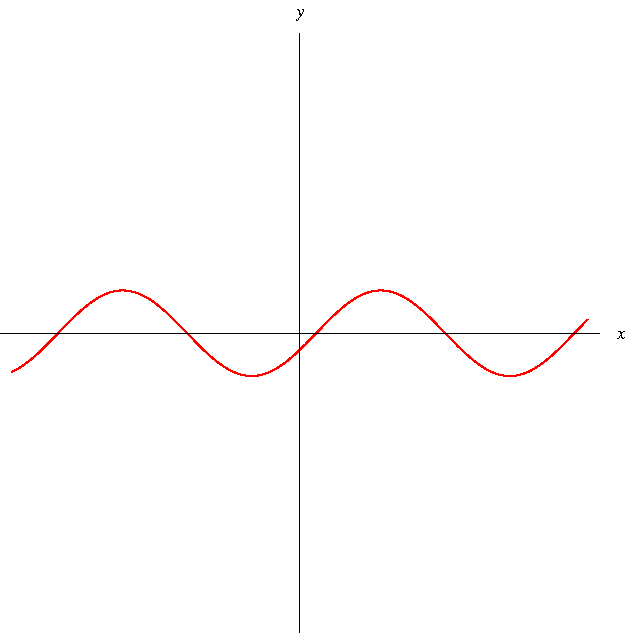
\includegraphics[height=3.8cm]{precalculus/pictures/01-02-vlt3.pdf} 
&%
\psset{xunit=0.33cm, yunit=0.33cm}
\begin{pspicture}(-5, -5)(5,5) 
\psframe*[linecolor=white](-5,-5)(5,5) 
\psaxes[ticks=none, labels=none]{<->}(0,0)(-4.5,-4.5)(4.5,4.5)\parametricplot[linecolor=red, plotpoints=1000]{0.05}{3}{t t 2.2 mul 57.29578 mul sin 1 add add t 57.29578 mul cos mul t t 2.2 mul 57.29578 mul sin 1 add add t 57.29578 mul sin mul}
\only<handout| 6->{%
\psline(1.7, -4.5)(1.7, 4.5)
}
\end{pspicture}
%\only<handout:0| -2>{%
%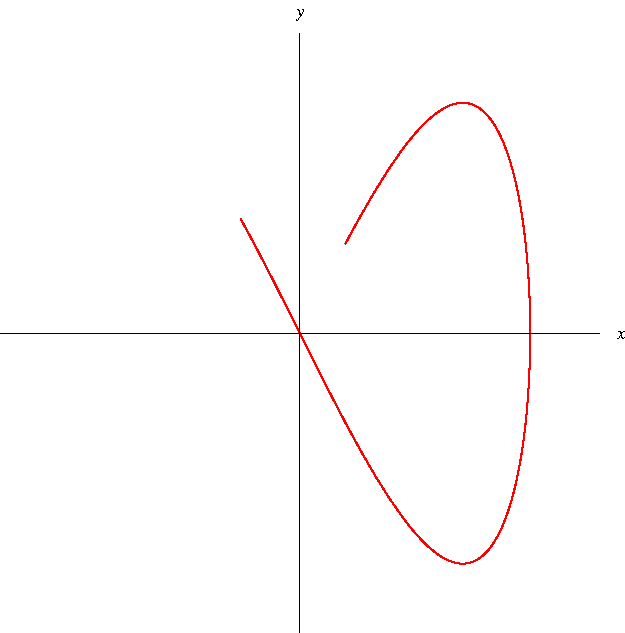
\includegraphics[height=3.8cm]{precalculus/pictures/01-02-vlt1a.pdf}%
%}%
%\only<handout| 3->{%
%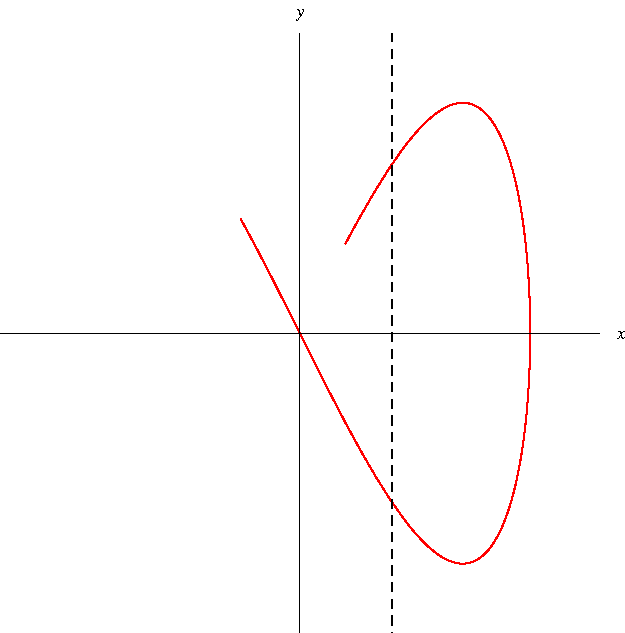
\includegraphics[height=3.8cm]{precalculus/pictures/01-02-vlt1b.pdf}%
%} 
&%
\psset{xunit=0.33cm, yunit=0.33cm}
\begin{pspicture}(-5, -5)(5,5) 
\psframe*[linecolor=white](-5,-5)(5,5) 
\psaxes[ticks=none, labels=none]{<->}(0,0)(-4.5,-4.5)(4.5,4.5)\tiny
%Function formula: 3/8+3/2 ((x)^{2})+1/4 (x)- ((x)^{3}) 
\psplot[linecolor=red, plotpoints=1000]{-0.5}{2}{x 3 exp -1 mul x 0.25 mul x 2 exp 1.5 mul 0.375 add add add } %Function formula: 1+1/2 (x) 
\psplot[linecolor=red, plotpoints=1000]{-4}{-0.5}{x 0.5 mul 1 add }
\end{pspicture} 
%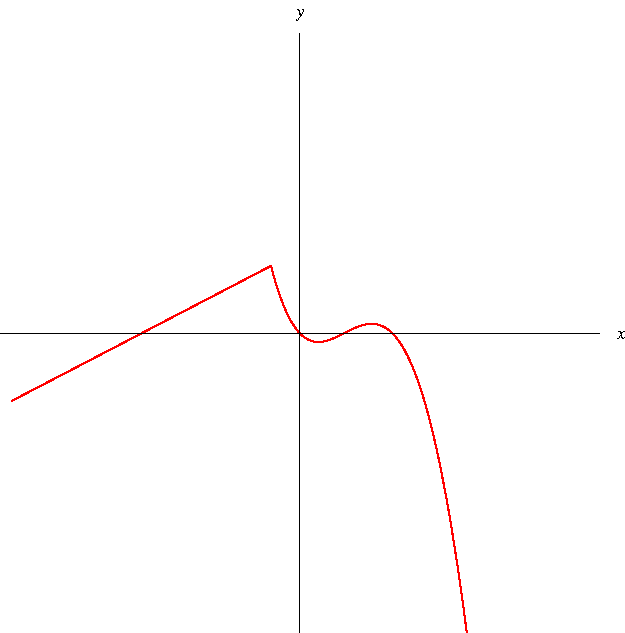
\includegraphics[height=3.8cm]{precalculus/pictures/01-02-vlt2.pdf} 
\\%
\fcAnswerUncoverNoH{1}{4}{Function} &
\fcAnswerUncoverNoH{1}{6}{Not a function}&
\fcAnswerUncoverNoH{1}{8}{Function}
\end{tabular}
\end{frame}
% end module vertical-line-test

\subsection{Piecewise Defined Functions}
% begin module function-piecewise
\begin{frame}
\frametitle{Piecewise Defined Functions}
\begin{definition}[Piecewise Defined Function]
A piecewise defined function is a function that is defined by different algebraic formulas on different subsets of its domain.
\end{definition}
\uncover<2->{
\begin{example}
\begin{columns}[t]
\column{.4\textwidth}
\psset{xunit=0.8cm, yunit=0.8cm}
\begin{pspicture}(-5, -5)(5,5) 
\psframe*[linecolor=white](-5,-5)(5,5) 
\psaxes[ticks=none, labels=none]{<->}(0,0)(-3,-1.5)(3,1.5)\tiny
\psLabelsWithOnes{3}{1.5}
\psline[linecolor=red](-3, -1)(0,-1)
\psline[linecolor=red](3, 1)(0,1)
\psHollowDot{0}{-1}
\psFullDot{0}{1}
\end{pspicture} 
%\ 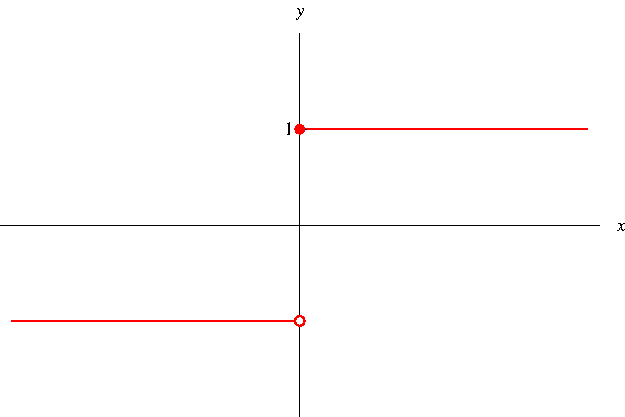
\includegraphics[height=3.5cm]{precalculus/pictures/01-01-piecewise.pdf}
\column{.5\textwidth}
\[
f(x) = \left\{ \begin{array}{rcc}
1 & \textrm{ if } & x \geq 0 \\
-1 & \textrm{ if } & x < 0 
\end{array}\right. 
\]

The filled red circle means $(0,1)$ is on the curve.  

The open circle means $(0, -1)$ is not on the curve.
\end{columns}
\end{example}
}
\end{frame}
% end module function-piecewise

% begin module absolute-value
\begin{frame}
\begin{example}
The absolute value $|x|$ of a number $a$ is defined to be
\[
|x| = \left\{ \begin{array}{ccccl}
\alertNoH{ 2-3}{x} & \alertNoH{ 3}{\text{if}} & \alertNoH{ 3}{x} & \alertNoH{ 3}{\geq} & \alertNoH{ 3}{0} \\
\alertNoH{ 4-5}{-x} & \alertNoH{ 5}{\text{if}} &  \alertNoH{ 5}{x} & \alertNoH{ 5}{<} & \alertNoH{ 5}{0}. \end{array}\right.
\]

Sketch a graph of the function $f(x) = |x|$.

%no begin{center} due to bug!
\hfil\hfil
\psset{xunit=1.2cm, yunit=1.2cm}
\begin{pspicture}(-3.2, -0.5)(3.2,3.2)
\tiny
\psframe*[linecolor=white](-3.2,-0.5)(3.2,3.2)
\psaxes[ticks=none, labels=none]{<->}(0,0)(-3,-0.5)(3,3)
\fcLabelsWithOnes{3}{3}
\uncover<handout:0|2>{
\psline[linecolor=blue](-0.5, -0.5)(3,3)
}
\uncover<3->{
\psline[linecolor=red](0,0)(3,3)
}
\uncover<handout:0|4>{
\psline[linecolor=blue](-3, 3)(0.5,-0.5)
}
\uncover<5->{
\psline[linecolor=red](-3, 3)(0,0)
}
\end{pspicture}
\end{example}
\end{frame}
% end module absolute-value

% begin module piecewise-formula
\begin{frame}
\begin{example} %[Example 9, p. 18]
Find a formula for the function $f$ in the graph.

\psset{xunit=1.2cm, yunit=1.2cm}
\begin{pspicture}(-0.5, -0.5)(5.3,2.4)
\tiny
\psframe*[linecolor=white](-0.5,-0.5)(5.2,2.4)
\psaxes{<->}(0,0)(-0.5,-0.5)(5.2,2.2)
\fcLabels{5.1}{2.2}
\psline[linecolor=red](0,0)(1,1)(2,0)(5,0)
\fcHollowDot{5}{0}
\fcFullDot{0}{0}
\only<handout:0|4-5>{
\psline[linecolor=blue](-0.5, -0.5)(2,2)
}
\only<handout:0|6-7>{
\psline[linecolor=blue](-0.2, 2.2)(2.5,-0.5)
}
\only<handout:0|8-9>{
\psline[linecolor=blue](2, 0)(5,0)
}
\end{pspicture}
%\ \only<1-3,10>{%
%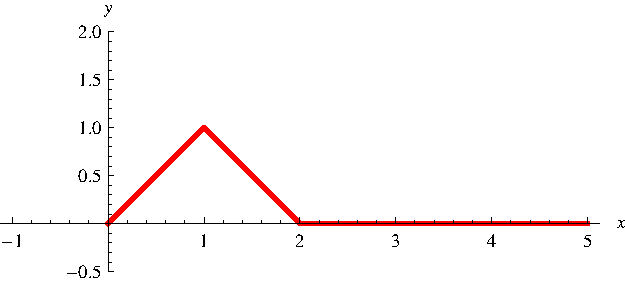
\includegraphics[height=4cm]{precalculus/pictures/01-01-ex-09a.pdf}%
%}%
%\only<handout:0| 4-5>{%
%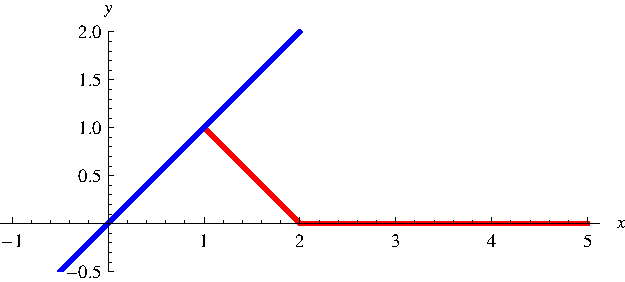
\includegraphics[height=4cm]{precalculus/pictures/01-01-ex-09b.pdf}%
%}%
%\only<handout:0| 6-7>{%
%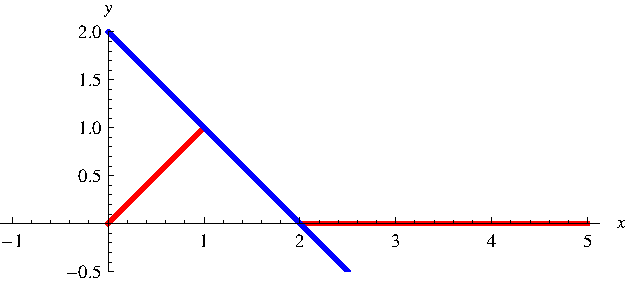
\includegraphics[height=4cm]{precalculus/pictures/01-01-ex-09c.pdf}%
%}%
%\only<handout:0| 8-9>{%
%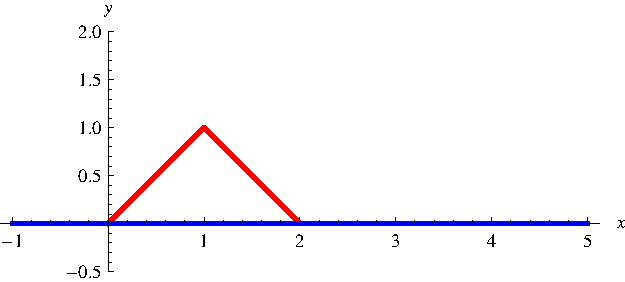
\includegraphics[height=4cm]{precalculus/pictures/01-01-ex-09d.pdf}%
%}%

\uncover<2->{
Different formulas on $[0, 1)$, $[1, 2)$, and $[2, 5)$.
}

\uncover<3->{
\[
f(x) = \left\{ \begin{array}{ccccccl}
\uncover<5->{\alert<handout:0| 5>{x}} & \alert<handout:0| 4-5>{\textrm{if}} & \alert<handout:0| 4-5>{0} & \alert<handout:0| 4-5>{\leq} & \alert<handout:0| 4-5>{x} & \alert<handout:0| 4-5>{<} & \alert<handout:0| 4-5>{1} \\
\uncover<7->{\alert<handout:0| 7>{2 - x}} & \alert<handout:0| 6-7>{\textrm{if}} & \alert<handout:0| 6-7>{1} & \alert<handout:0| 6-7>{\leq} & \alert<handout:0| 6-7>{x} & \alert<handout:0| 6-7>{<} & \alert<handout:0| 6-7>{2} \\
\uncover<9->{\alert<handout:0| 9>{0}} & \alert<handout:0| 8-9>{\textrm{if}} & \alert<handout:0| 8-9>{2} & \alert<handout:0| 8-9>{\leq} & \alert<handout:0| 8-9>{x} & \alert<handout:0| 8-9>{<} & \alert<handout:0| 8-9>{5} \end{array}\right.
\]
}
\end{example}
\end{frame}
% end module piecewise-formula

% begin module piecewise-ex1
\begin{frame}
\begin{example}
Sketch the function $f(x)  = |2x-3|$.
\begin{columns}
\column{.4\textwidth}
\only<-5| handout:0>{%
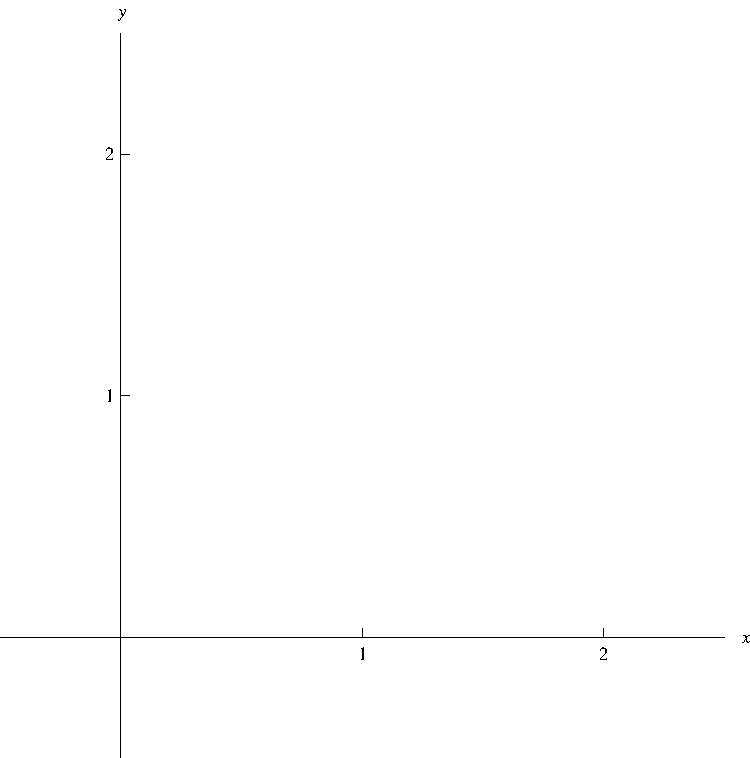
\includegraphics[width=4.5cm]{precalculus/pictures/piecewise-ex1-1.pdf}%
}%
\only<6| handout:0>{%
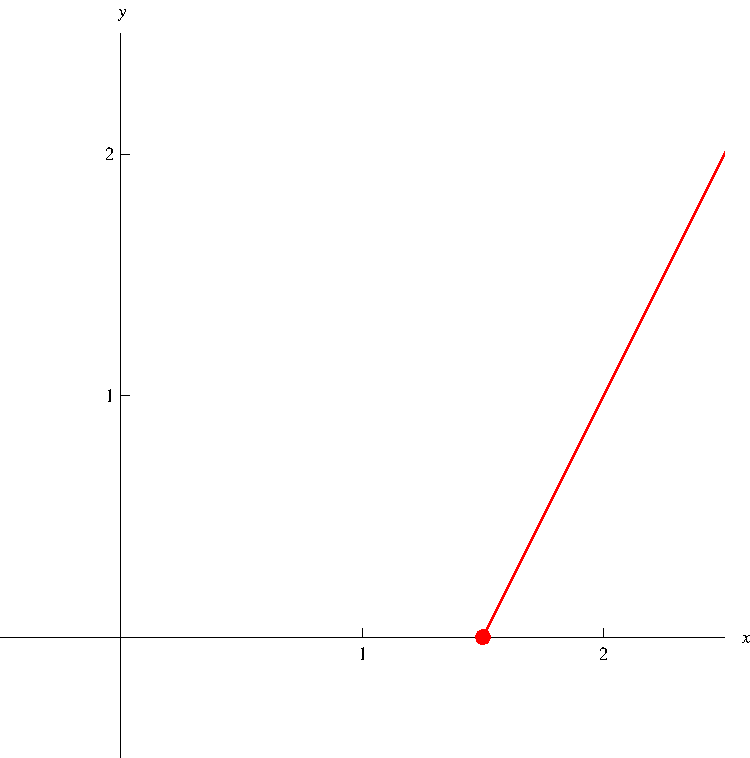
\includegraphics[width=4.5cm]{precalculus/pictures/piecewise-ex1-2.pdf}%
}%
\only<7-| handout:1>{%
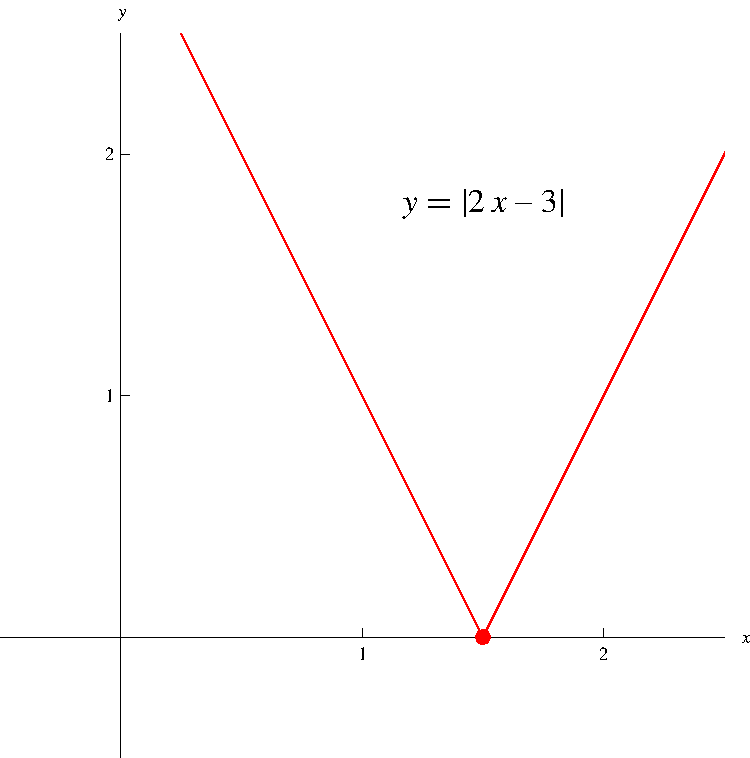
\includegraphics[width=4.5cm]{precalculus/pictures/piecewise-ex1-3.pdf}%
}%
\column{.55\textwidth}
\abovedisplayskip=0pt
\belowdisplayskip=-15pt
\abovedisplayshortskip=0pt
\belowdisplayshortskip=0pt
\begin{align*}
\uncover<2->{%
|\alert<handout:0| 3>{x}| %
}%
& \uncover<2->{%
 = \begin{cases}
\alert<handout:0| 3>{x} & \text{if $\alert<handout:0| 3>{x} \geq 0$}\\
-\alert<handout:0| 3>{x} & \text{if $\alert<handout:0| 3>{x} < 0$}.\\
\end{cases}
}\\%
\uncover<3->{%
|\alert<handout:0| 3>{2x-3}| %
}%
& \uncover<3->{%
 = \begin{cases}
\alert<handout:0| 3>{2x-3} & \text{if $\alert<handout:0| 3>{2x-3} \geq 0$}\\
-(\alert<handout:0| 3>{2x-3}) & \text{if $\alert<handout:0| 3>{2x-3} < 0$}\\
\end{cases}
}\\%
& \uncover<4->{%
 = \begin{cases}
2x-3 & \text{if $2x \geq 3$}\\
-2x+3 & \text{if $2x < 3$}\\
\end{cases}
}\\%
& \uncover<5->{%
 = \begin{cases}
\alert<handout:0| 6>{2x-3} & \alert<handout:0| 6>{\text{if $x \geq 3/2$}}\\
\alert<handout:0| 7>{-2x+3} & \alert<handout:0| 7>{\text{if $x < 3/2$}}.\\
\end{cases}
}%
\end{align*}
\end{columns}
\end{example}
\end{frame}
% end module piecewise-ex1

% begin module piecewise-ex2
\begin{frame}
\begin{example}
Sketch the function $\displaystyle f(x)  = \frac{|4x+2|}{2x+1}$.
\begin{columns}
\column{.4\textwidth}
\only<-8| handout:0>{%
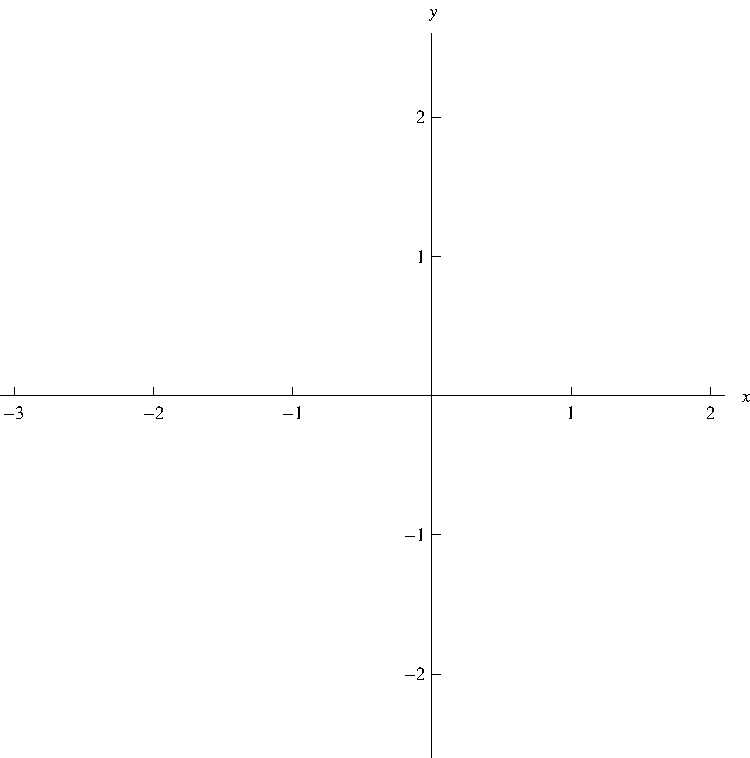
\includegraphics[width=4.5cm]{precalculus/pictures/piecewise-ex2-1.pdf}%
}%
\only<9| handout:0>{%
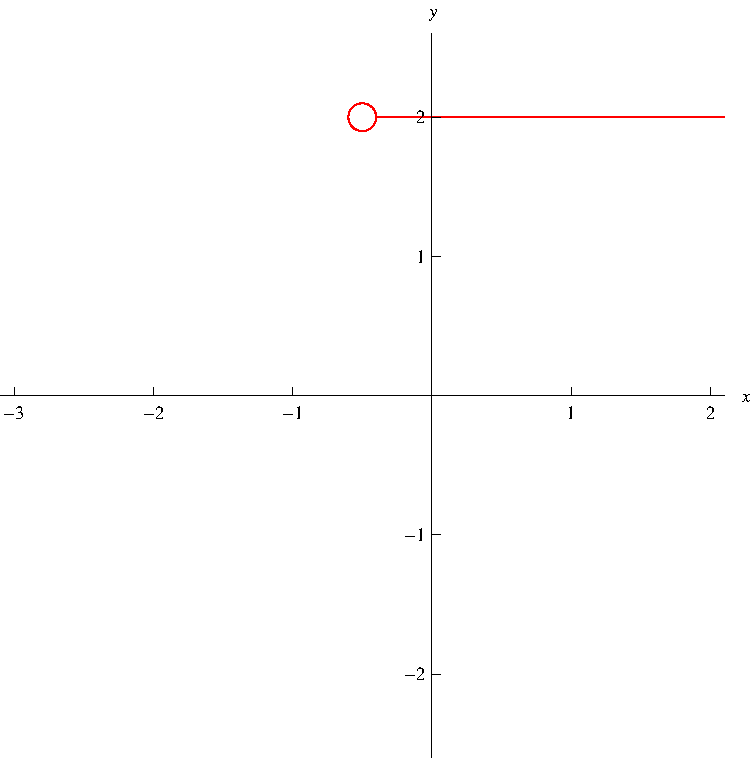
\includegraphics[width=4.5cm]{precalculus/pictures/piecewise-ex2-2.pdf}%
}%
\only<10-| handout:1>{%
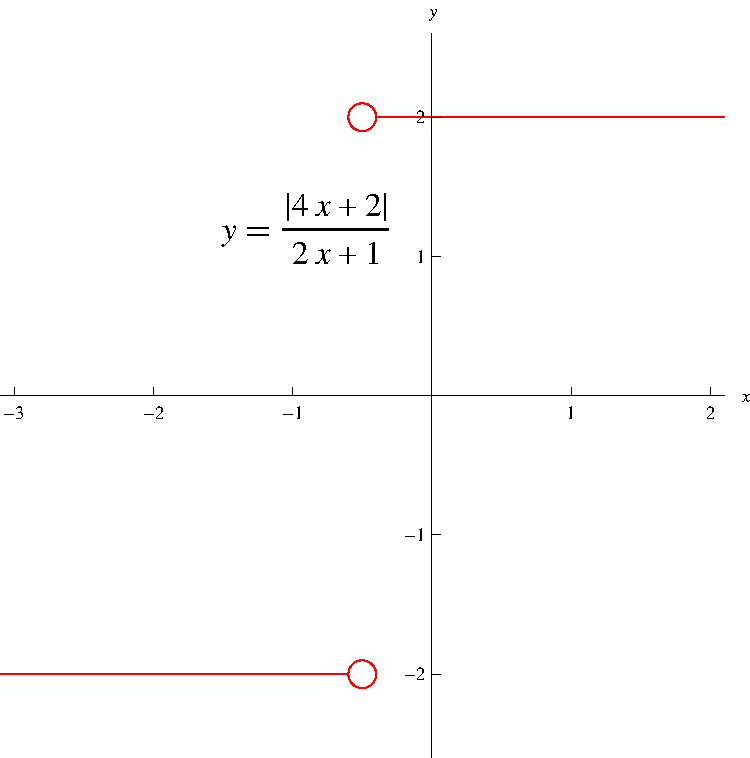
\includegraphics[width=4.5cm]{precalculus/pictures/piecewise-ex2-3.pdf}%
}%
\column{.55\textwidth}
\abovedisplayskip=0pt
\belowdisplayskip=-15pt
\abovedisplayshortskip=0pt
\belowdisplayshortskip=0pt
\begin{align*}
\uncover<2->{%
|\alert<handout:0| 3>{x}| %
}%
& \uncover<2->{%
 = \begin{cases}
\alert<handout:0| 3>{x} & \text{if $\alert<handout:0| 3>{x} \geq 0$}\\
-\alert<handout:0| 3>{x} & \text{if $\alert<handout:0| 3>{x} < 0$}.\\
\end{cases}
}\\%
\uncover<3->{%
\frac{|\alert<handout:0| 3>{4x+2}|}{2x+1} %
}%
& \uncover<3->{%
 = \begin{cases}
\frac{\alert<handout:0| 3-5>{4x+2}}{2x+1} & \text{if $\alert<handout:0| 3>{4x+2} > 0$}\\
\frac{\alert<handout:0| 6-7>{-(\alert<handout:0| 3>{4x+2})}}{2x+1} & \text{if $\alert<handout:0| 3>{4x+2} < 0$}\\
\end{cases}
}\\%
& \uncover<4->{%
 = \begin{cases}
\frac{\uncover<5->{\alert<handout:0| 5>{2(2x+1)}}}{2x+1} & \text{if $4x > -2$}\\
\frac{\uncover<7->{\alert<handout:0| 7>{-2(2x+1)}}}{2x+1} & \text{if $4x < -2$}\\
\end{cases}
}\\%
& \uncover<8->{%
 = \begin{cases}
\alert<handout:0| 9>{2} & \alert<handout:0| 9>{\text{if $x > -1/2$}}\\
\alert<handout:0| 10>{-2} & \alert<handout:0| 10>{\text{if $x < -1/2$}}.\\
\end{cases}
}%
\end{align*}
\end{columns}
\end{example}
\end{frame}
% end module piecewise-ex2

\subsection{Zeroes of a function}
\begin{frame}

\begin{definition}
The zeroes of a function $f$ are the values of the argument $x$ for which $f(x)=0$.
\end{definition}

\begin{observation}
The zeroes of a function are the $x$-coordinates of the $x$ intercepts of the graph of the function.
\end{observation}

\begin{pspicture}(-1.2,-1.2)(1.2,1.1)
\fcAxesStandard{-1.2}{-1.2}{1.2}{1.2}
\psplot[linecolor=\fcColorGraph]{-1.2}{1.2}{x 1 sub x x 1 add mul mul}
\fcFullDot{0}{0}
\fcFullDot{1}{0}
\fcFullDot{-1}{0}
\end{pspicture}


\end{frame}
\begin{frame}

\begin{example}
\begin{columns}
\column{0.45\textwidth}
\begin{pspicture}(-1,-1)(1,1)
\fcAxesStandard{-3.2}{-2}{2.2}{2}
\psplot[linecolor=\fcColorGraph]{-3.2}{2.2}{1 6 div x x x mul mul mul 1 6 div x x mul mul -1 x mul add add }
\uncover<2->{
\fcFullDot{-3}{0}
\fcFullDot{2}{0}
\fcFullDot{0}{0}
}
\end{pspicture}
\column{0.55\textwidth}
Find the zeroes of $\displaystyle  f(x)=\frac{1}{6}x^3+\frac{1}{6}x^2-x$.

\end{columns}
\uncover<2->{}
\end{example}
\end{frame}
\begin{frame}
\begin{example}
\begin{itemize}
\item Find when $f(x)=g(x)$, where 
\[
f(x)=\frac{1}{6}x^3+\frac{1}{6}x^2\qquad \qquad g(x)=x
\]
\item Find the intersections of the graphs of $f$ and $g$.
\end{itemize}
\end{example}
\end{frame}
\begin{frame}
Let $g$ of $x$ and $f$ of $x$ be functions.
\begin{columns}

\column{0.45\textwidth}
\psset{xunit=0.5cm, yunit=0.5cm}
\begin{pspicture}(-4,-4)(2.2,3)
\tiny
\fcAxesStandard{-4}{-4}{2.2}{3}
\uncover<2->{
\psplot[linecolor=\fcColorGraph]{-3.2}{2.2}{1 6 div x x x mul mul mul 1 6 div x x mul mul add }
\rput[l](-2,1){$f(x)=\frac{1}{6}x^3+\frac{1}{6}x^2$}
}
\uncover<3->{
\psline[linecolor=\fcColorGraph](-3.2,-3.2)(2.2,2.2)
\rput[t](-1,-2){$g(x)=x$}
}
\uncover<4->{
\fcFullDot{-3}{-3}
\fcFullDot{0}{0}
\fcFullDot{2}{2}
}
\uncover<5->{
\rput[l](-3,-3){$~~(\alertNoH{5,10}{-3}, -3)$}
\rput[tl](0,-0.1){$~~(\alertNoH{5,10}{0}, 0)$}
\rput[r](2,2){$(\alertNoH{5,10}{2}, 2)~~$}
}
\end{pspicture}
\psset{xunit=0.5cm, yunit=0.5cm}
\begin{pspicture}(-4,-4)(2.2,3)
\tiny
\fcAxesStandard{-4}{-4}{2.2}{3}
\uncover<8->{
\psplot[linecolor=\fcColorGraph]{-3.2}{2.2}{1 6 div x x x mul mul mul 1 6 div x x mul mul add -1 x mul add}
}
\uncover<7->{%
\rput(-1,2){$f(x)-g(x)=\frac{1}{6}x^3+\frac{1}{6}x^2-x$}
}%
\uncover<9->{
\fcFullDot{-3}{0}
\fcFullDot{2}{0}
\fcFullDot{0}{0}
}
\uncover<10->{
\rput[tl](-3, -0.1){$(\alertNoH{10}{-3},0)$}
\rput[tl](0, -0.1){$~~(\alertNoH{10}{0},0)$}
\rput[br](2, 0.1){$(\alertNoH{10}{2},0)~~$}
}
\end{pspicture}
\column{0.55\textwidth}
\begin{observation}
\begin{itemize}
\item To solve $\alertNoH{2}{f(x)}=\alertNoH{3}{g(x)}$ means to find the \alertNoH{5}{$x$ coordinates} of the \alertNoH{4}{intersections of the graphs of $f$ and $g$}. 
\item<6-> To solve $f(x)=g(x)$ is equivalent to solving the equation $f(x)-g(x)=0$.
\item<7-> To solve $f(x)=g(x) $ means to find \alertNoH{9}{the zeroes} of $\alertNoH{7,8}{f(x)-g(x)}$.
\item<10-> The \alertNoH{10}{$x$ coordinates of the intersections of $f(x)$ and $g(x)$} coincide with the \alertNoH{10}{$x$ coordinates of the $x$ intercepts of $f(x)-g(x)$}.
\end{itemize}
\end{observation}
\end{columns}
\end{frame}
\subsection{Symmetry}
% begin module even-and-odd
\begin{frame}
\frametitle{Symmetry}
\begin{definition}[Even and Odd Functions]
A function $f$ is called even if $f(-x) = f(x)$ for all $x$ in its domain.  A function $f$ is called odd if $f(-x) = -f(x)$ for all $x$ in its domain.
\end{definition}
\uncover<2->{
\begin{example}[$x^2$ is Even, $x^3$ is Odd]
The function $f(x) = x^2$ is even:
\uncover<3->{
\[
f(-x) = (-x)^2 = x^2 = f(x) .
\]
}
The function $g(x) = x^3$ is odd:
\uncover<4->{
\[
g(-x) = (-x)^3 = -x^3 = -g(x) .
\]
}
\end{example}
}
\end{frame}

\begin{frame}
\begin{definition}[Even and Odd Functions]
A function $f$ is called even if $f(-x) = f(x)$ for all $x$ in its domain.  A function $f$ is called odd if $f(-x) = -f(x)$ for all $x$ in its domain.
\end{definition}
\begin{example} %[Example 11, p. 19]
Determine whether each of the following functions is even, odd, or neither even nor odd.

\begin{columns}[t]
\column{.33\textwidth}
\[
f(x) = x^5 + x
\]
\[
\begin{array}{r@{ \ }c@{ \ }l}
\uncover<2->{f(-x)} & \uncover<2->{=} & \uncover<3->{(-x)^5 + (-x)} \\
& \uncover<4->{=} & \uncover<4->{-x^5 - x} \\
& \uncover<5->{=} & \uncover<5->{-(x^5 + x)} \\
& \uncover<6->{=} & \uncover<6->{-f(x)} 
\end{array}
\]
\uncover<7->{
Therefore $f$ is odd.
}
\column{.33\textwidth}
\[
g(x) = 1 - x^4
\]
\[
\begin{array}{r@{ \ }c@{ \ }l}
\uncover<2->{g(-x)} & \uncover<2->{=} & \uncover<8->{1 - (-x)^4} \\
& \uncover<9->{=} & \uncover<9->{1 - x^4} \\
& \uncover<10->{=} & \uncover<10->{g(x)} 
\end{array}
\]
\uncover<11->{
Therefore $g$ is even.
}
\column{.33\textwidth}
\[
h(x) = 2x - 1
\]
\[
\begin{array}{r@{ \ }c@{ \ }l}
\uncover<2->{h(-x)} & \uncover<2->{=} & \uncover<12->{2(-x) - 1} \\
& \uncover<13->{=} & \uncover<13->{-2x - 1} \\
& \uncover<14->{\neq} & \uncover<14->{h(x), -h(x)}
\end{array}
\]
\uncover<15->{
Therefore $h$ is neither even nor odd.
}
\end{columns}
\end{example}
\end{frame}
% end module even-and-odd

\subsection{Increasing and Decreasing Functions}
% begin module increasing-decreasing
\begin{frame}
\frametitle{Increasing and Decreasing Functions}
\begin{definition}[Increasing and Decreasing Functions]
A function $f$ is called increasing on an interval $I$ if $f(x_1) < f(x_2)$ whenever $x_1 < x_2$  in $I$.

It is called decreasing on the interval $I$ if $f(x_1) > f(x_2)$ whenever $x_1 < x_2$ in $I$.
\end{definition}
\uncover<2->{
\begin{example}[Increasing and Decreasing]
\begin{columns}[t]
\column{.6\textwidth}

\psset{xunit=3.4cm, yunit=3.4cm}
\begin{pspicture}(-1.1, -0.4)(1.15,0.7)
\psframe*[linecolor=white](-1.1,-0.4)(1.15,0.7)
\tiny
\psaxes[Dx=0.25, Dy=0.25]{<->}(0,0)(-1.1,-0.3)(1.1,0.6)
\fcLabels{1.1}{0.6}
%Function formula: 7/40+13/10 ((x)^{3})-39/40 (x)
\psplot[linecolor=red, plotpoints=1000]{-1}{1}{x -0.975 mul x 3 exp 1.3 mul 0.175 add add }
\uncover<handout:0|3>{
\psplot[linecolor=blue, plotpoints=1000]{-1}{-0.5}{x -0.975 mul x 3 exp 1.3 mul 0.175 add add }
}
\uncover<handout:0|4>{
\psplot[linecolor=blue, plotpoints=1000]{-0.5}{0.5}{x -0.975 mul x 3 exp 1.3 mul 0.175 add add }
}
\uncover<handout:0|5>{
\psplot[linecolor=blue, plotpoints=1000]{0.5}{1}{x -0.975 mul x 3 exp 1.3 mul 0.175 add add }
}
\end{pspicture}
%\ \only<-2>{%
%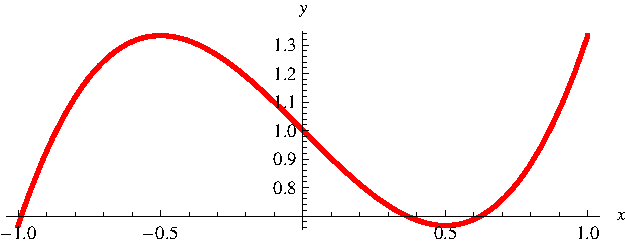
\includegraphics[height=2.8cm]{precalculus/pictures/01-01-inc-dec-a.pdf}%
%}%
%\only<handout:0| 3>{%
%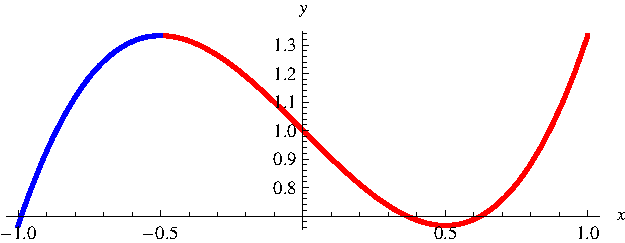
\includegraphics[height=2.8cm]{precalculus/pictures/01-01-inc-dec-b.pdf}%
%}%
%\only<handout:0| 4>{%
%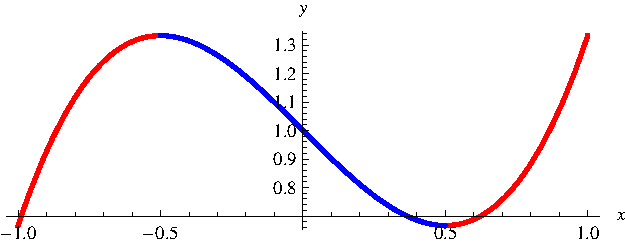
\includegraphics[height=2.8cm]{precalculus/pictures/01-01-inc-dec-c.pdf}%
%}%
%\only<handout:0| 5->{%
%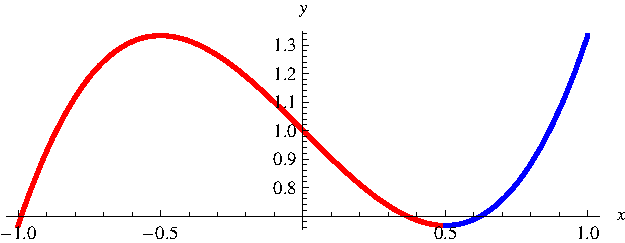
\includegraphics[height=2.8cm]{precalculus/pictures/01-01-inc-dec-d.pdf}%
%}%
\column{.4\textwidth}
\begin{itemize}
\item<3-| alert@3> \only<handout:0|3>{\color{blue}} $f$ is increasing on $[-1, -\frac{1}{2}]$.
\item<4-| alert@4> \only<handout:0|4>{\color{blue}} $f$ is decreasing on $[-\frac{1}{2}, \frac{1}{2}]$.
\item<5-| alert@5> \only<handout:0|5>{\color{blue}} $f$ is increasing on $[\frac{1}{2}, 1]$.
\end{itemize}
\end{columns}
\end{example}
}
\end{frame}
% end module increasing-decreasing


}% end lecture

\lect{\semester}{Lecture  5}{5}{
%DesiredLectureName: Functions
\fcLicense
\section{A Catalog of Essential Functions}
\subsection{Linear Functions}
% begin module linear-functions
\begin{frame}
\frametitle{Linear Functions}
\begin{definition}[Linear Function]
A linear function is a function the graph of which is a line.  We can write any linear function in slope-intercept form:
\[
f(x) = mx + b.
\]
$m$ is called the slope, and $b$ is called the $y$-intercept.
\end{definition}
\end{frame}

\begin{frame}
\begin{columns}[c]
\column{.5\textwidth}

\psset{xunit=0.7cm, yunit=0.7cm}
\begin{pspicture}(-2.6, -2.5)(5,2.6)
\psframe*[linecolor=white](-2.6,-2.5)(4.1,2.6)
\tiny
\fcAxesStandard{-2.6}{-2.5}{5}{2.6}
\fcLabelXOne
\uncover<2>{
\psline[linecolor=red](-2.5, -1.5)(1.5, 2.5)
}
\uncover<3->{
\psline[linecolor=blue](-2.5, -1.5)(1.5, 2.5)
}
\uncover<2->{
\rput[l](1.5, 2){$y=x+1$}
}
\uncover<5->{
\fcFullDot{0}{1}
\rput[r](-0.1, 1){\alert<5>{$(0,1)$}}
}

\uncover<3>{
\psline[linecolor=red](-2.5, 1.25)(5, -2.5)
}
\uncover<4->{
\psline[linecolor=blue](-2.5, 1.25)(5, -2.5)
}
\uncover<3->{
\rput[r](3.3, -2){$y=-0.5x$}
}
\uncover<6->{
\fcFullDot{0}{0}
\rput[lb](0.1, 0.1){\alert<6>{$(0,0)$}}
}

\uncover<4>{
\psline[linecolor=red](-2.5,-1)(5, -1)
}
\uncover<5->{
\psline[linecolor=blue](-2.5, -1)(5, -1)
}
\uncover<4->{
\rput[t](4, -1.1){$y=-1$}
}
\uncover<7->{
\fcFullDot{0}{-1}
\rput[lt](0.1, -1.1){\alert<7>{$(0,-1)$}}
}
\end{pspicture}
\column[t]{.55\textwidth}
\begin{tabular}{|c|c|c|}
\hline
$f(x)$ & Direction & $y$-intercept \\
\hline
\uncover<1->{\alert<handout:0| 2>{$x + \alert<handout:0| 5>{1}$}} &
\uncover<2->{\alert<handout:0| 2>{$\nearrow$}} &
\uncover<5->{\alert<handout:0| 5>{1}} \\
\uncover<1->{\alert<handout:0| 3>{$-0.5x \uncover<6>{\alert<handout:0| 6>{+ 0}}$}} &
\uncover<3->{\alert<handout:0| 3>{$\searrow$}} &
\uncover<6->{\alert<handout:0| 6>{0}} \\
\uncover<1->{\alert<handout:0| 4,7>{$-1$}} &
\uncover<4->{\alert<handout:0| 4>{$\rightarrow$}} &
\uncover<7->{\alert<handout:0| 7>{-1}} \\
\hline
\end{tabular}
\end{columns}

\begin{itemize}
\item<2->  $m > 0$ means the graph of $f$ points up ($\nearrow$).
\item<3->  $m < 0$ means the graph of $f$ points down ($\searrow$).
\item<4->  $m = 0$ means the graph of $f$ is horizontal ($\rightarrow$).
\item<5->  $b$ tells us the height of the point where the graph hits the $y$-axis.
\end{itemize}
\end{frame}
% end module linear-functions

%\begin{frame}
\begin{columns}[c]
\column{.5\textwidth}

\psset{xunit=0.7cm, yunit=0.7cm}
\begin{pspicture}(-2.6, -2.5)(4.1,2.6)
\psframe*[linecolor=white](-2.6,-2.5)(4.1,2.6)
\tiny
\fcAxesStandard{-2.6}{-2.5}{5}{2.6}
\fcLabelXOne
\uncover<2>{
\psline[linecolor=red](-2.5, -1.5)(1.5, 2.5)
}
\uncover<3->{
\psline[linecolor=blue](-2.5, -1.5)(1.5, 2.5)
}
\uncover<2->{
\rput[l](1.5, 2){$y=x+1$}
}
\uncover<5->{
\fcFullDot{0}{1}
\rput[r](-0.1, 1){\alert<5>{$(0,1)$}}
}

\uncover<3>{
\psline[linecolor=red](-2.5, 1.25)(5, -2.5)
}
\uncover<4->{
\psline[linecolor=blue](-2.5, 1.25)(5, -2.5)
}
\uncover<3->{
\rput[r](3.3, -2){$y=-0.5x$}
}
\uncover<6->{
\fcFullDot{0}{0}
\rput[lb](0.1, 0.1){\alert<6>{$(0,0)$}}
}

\uncover<4>{
\psline[linecolor=red](-2.5,-1)(5, -1)
}
\uncover<5->{
\psline[linecolor=blue](-2.5, -1)(5, -1)
}
\uncover<4->{
\rput[t](4, -1.1){$y=-1$}
}
\uncover<7->{
\fcFullDot{0}{-1}
\rput[lt](0.1, -1.1){\alert<7>{$(0,-1)$}}
}
\end{pspicture}
%\ \only<handout:0| -2>{%
%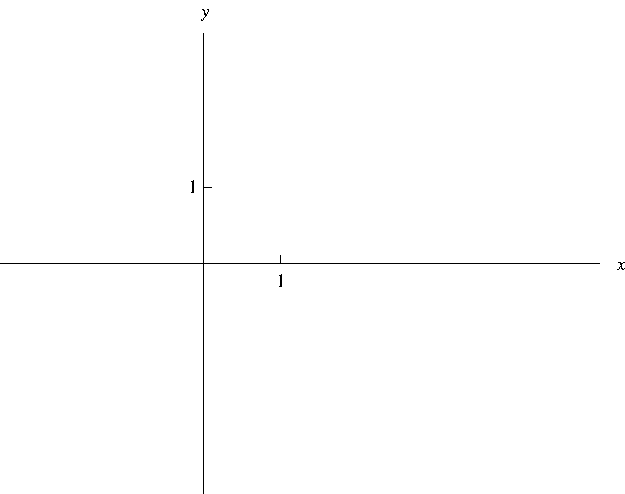
\includegraphics[height=4.5cm]{precalculus/pictures/01-02-linesa.pdf}%
%}%
%\only<handout:0| 3>{%
%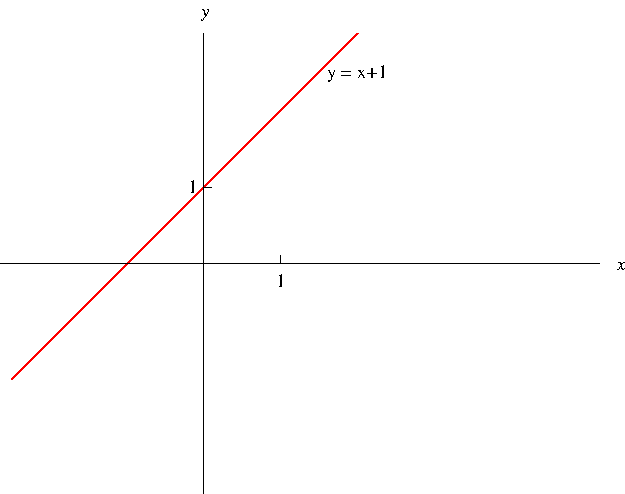
\includegraphics[height=4.5cm]{precalculus/pictures/01-02-linesb.pdf}%
%}%
%\only<handout:0| 4>{%
%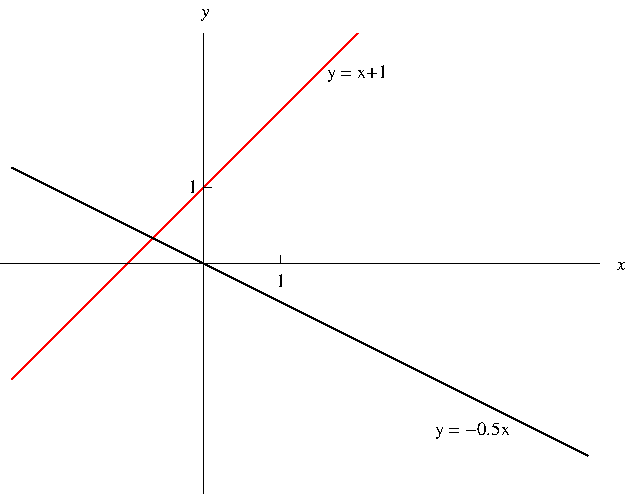
\includegraphics[height=4.5cm]{precalculus/pictures/01-02-linesc.pdf}%
%}%
%\only<handout:0| 5>{%
%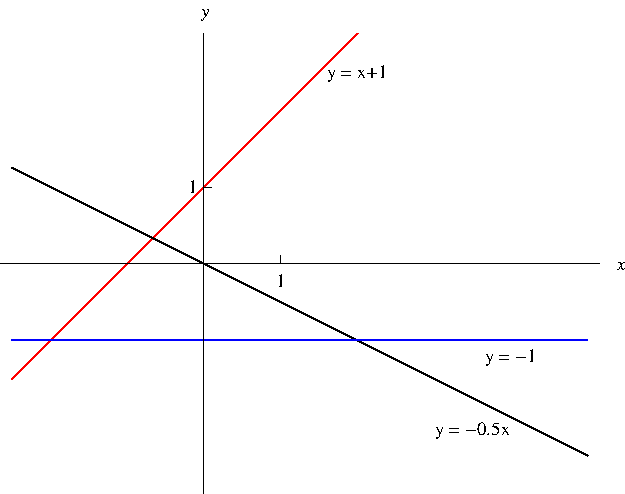
\includegraphics[height=4.5cm]{precalculus/pictures/01-02-linesd.pdf}%
%}%
%\only<handout:0| 6>{%
%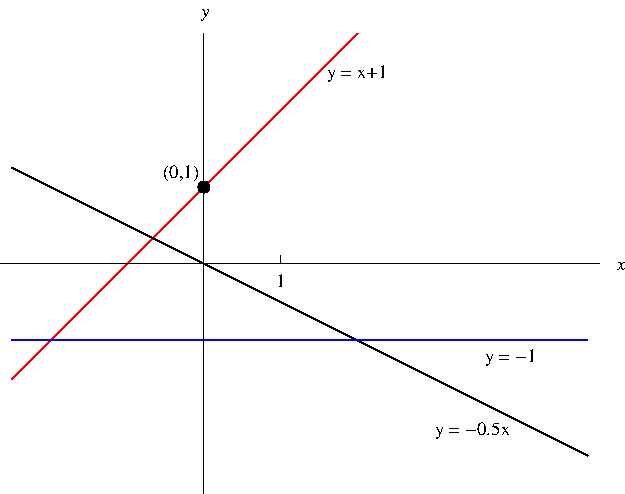
\includegraphics[height=4.5cm]{precalculus/pictures/01-02-linese.pdf}%
%}%
%\only<handout:0| 7>{%
%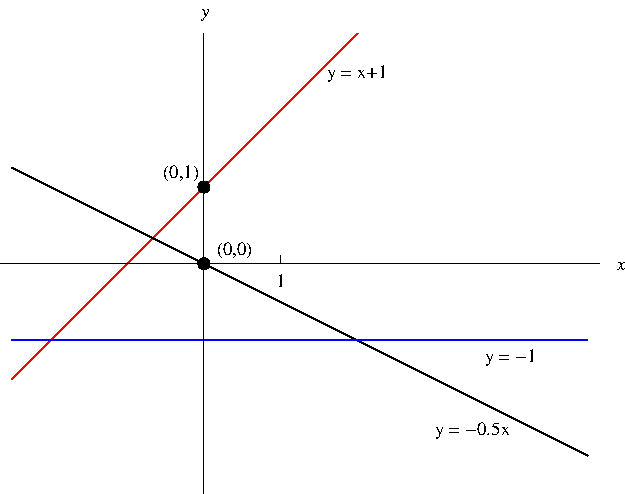
\includegraphics[height=4.5cm]{precalculus/pictures/01-02-linesf.pdf}%
%}%
%\only<8>{%
%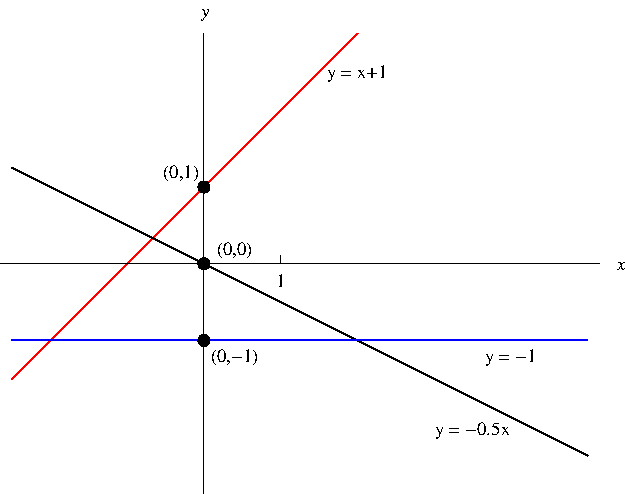
\includegraphics[height=4.5cm]{precalculus/pictures/01-02-linesg.pdf}%
%}%
\column[t]{.55\textwidth}
\begin{tabular}{|c|c|c|}
\hline
$f(x)$ & Direction & $y$-intercept \\
\hline
\uncover<1->{\alertNoH{ 2}{$x + \alertNoH{ 5}{1}$}} &
\uncover<2->{\alertNoH{ 2}{$\nearrow$}} &
\uncover<5->{\alertNoH{ 5}{1}} \\
\uncover<1->{\alertNoH{ 3}{$-0.5x \uncover<6>{\alertNoH{ 6}{+ 0}}$}} &
\uncover<3->{\alertNoH{ 3}{$\searrow$}} &
\uncover<6->{\alertNoH{ 6}{0}} \\
\uncover<1->{\alertNoH{ 4,7}{$-1$}} &
\uncover<4->{\alertNoH{ 4}{$\rightarrow$}} &
\uncover<7->{\alertNoH{ 7}{-1}} \\
\hline
\end{tabular}
\end{columns}

\begin{itemize}
\item<2->  $m > 0$ means the graph of $f$ points up ($\nearrow$).
\item<3->  $m < 0$ means the graph of $f$ points down ($\searrow$).
\item<4->  $m = 0$ means the graph of $f$ is horizontal ($\rightarrow$).
\item<5->  $b$ tells us the height of the point where the graph hits the $y$-axis.
\end{itemize}
\end{frame}
\subsection{Polynomials}
% begin module polynomials
\begin{frame}
\frametitle{Polynomials}
\begin{definition}[Polynomial Function]
A polynomial function is a function $f$ of the form
\[
f(x) = a_0 + a_1x + a_2x^2 + \cdots + a_{n - 1}x^{n-1} + a_nx^n ,
\]
where $n$ is a non-negative integer and $a_0, \ldots , a_n$ are real numbers, called the coefficients.

If the leading coefficient $a_n \neq 0$, then we say the degree of $f$ is $n$.
\end{definition}
\uncover<2->{
\[
\begin{array}{|c|c|c|c|c|c|}
\hline
f(x) &%
\alert<handout:0| 3-4,13-14,23-26,35-36>{\text{Polynomial?}} &%
\alert<handout:0| 5-6,15-16,27-28>{\text{Degree}} &%
\alert<handout:0| 7-8,17-18,29-30>{a_0} &%
\alert<handout:0| 9-10,19-20,31,32>{a_1} &%
\alert<handout:0| 11-12,21-22,33-34>{a_2} \\
\hline
\alert<handout:0| 3-12>{x^4-x+1} &%
\uncover<4->{\alert<handout:0| 4>{\text{Yes}}}&%
\uncover<6->{\alert<handout:0| 6>{4}}&%
\uncover<8->{\alert<handout:0| 8>{1}}&%
\uncover<10->{\alert<handout:0| 10>{-1}}&%
\uncover<12->{\alert<handout:0| 12>{0}}\\%
\alert<handout:0| 13-22>{6} &%
\uncover<14->{\alert<handout:0| 14>{\text{Yes}}}&%
\uncover<16->{\alert<handout:0| 16>{0}}&%
\uncover<18->{\alert<handout:0| 18>{6}}&%
\uncover<20->{\alert<handout:0| 20>{0}}&%
\uncover<22->{\alert<handout:0| 22>{0}}\\%
\alert<handout:0| 23>{3x^2 - \frac{1}{2}x + \alert<handout:0| 24>{\sqrt{x}}} &%
\uncover<24->{\alert<handout:0| 24>{\text{No}}}&%
&%
&%
&\\
\alert<handout:0| 25-34>{3x^2 - \frac{1}{2}x + \sqrt{2}} &%
\uncover<26->{\alert<handout:0| 26>{\text{Yes}}}&%
\uncover<28->{\alert<handout:0| 28>{2}}&%
\uncover<30->{\alert<handout:0| 30>{\sqrt{2}}}&%
\uncover<32->{\alert<handout:0| 32>{-\frac{1}{2}}}&%
\uncover<34->{\alert<handout:0| 34>{3}}\\%
\alert<handout:0| 35>{3x^2 - \frac{1}{2\alert<handout:0| 36>{x}} + \sqrt{2}} &%
\uncover<36->{\alert<handout:0| 36>{\text{No}}}&%
&%
&%
&\\
\hline
\end{array}
\]
}
\end{frame}


\begin{frame}
\begin{itemize}
\item<1->  Linear functions are polynomials.
\item<2->  So are quadratic functions.  Their graphs are parabolas.
\item<3->  And there are many more.
\end{itemize}
\only<handout:1| 1>{%
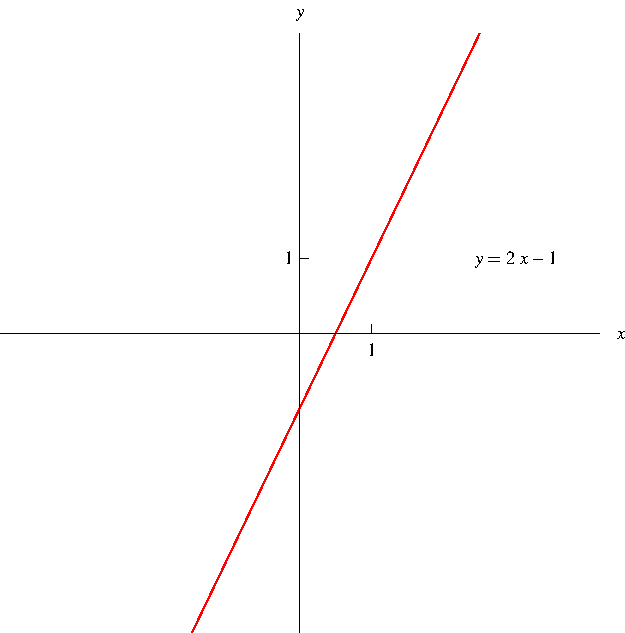
\includegraphics[height=6cm]{precalculus/pictures/01-02-line.pdf}%

Linear
}%
\only<handout:2| 2>{%
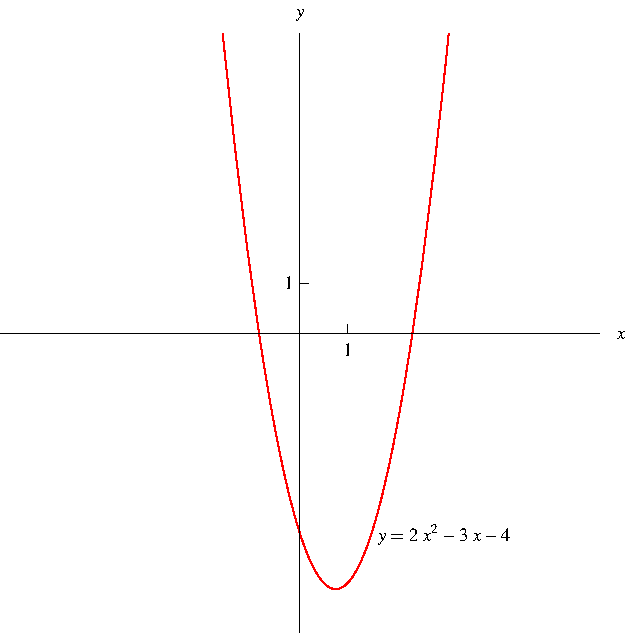
\includegraphics[height=6cm]{precalculus/pictures/01-02-parabola.pdf}%

Quadratic
}%
\only<handout:3| 3>{%
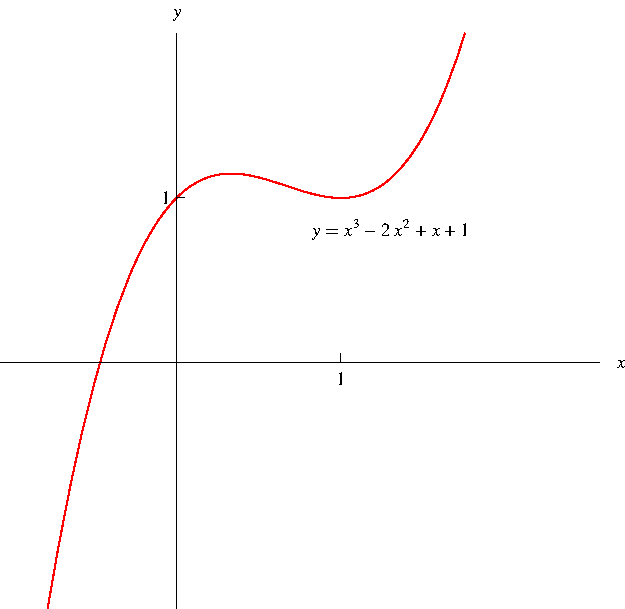
\includegraphics[height=6cm]{precalculus/pictures/01-02-polya.pdf}%

Cubic
}%
\only<handout:4| 4>{%
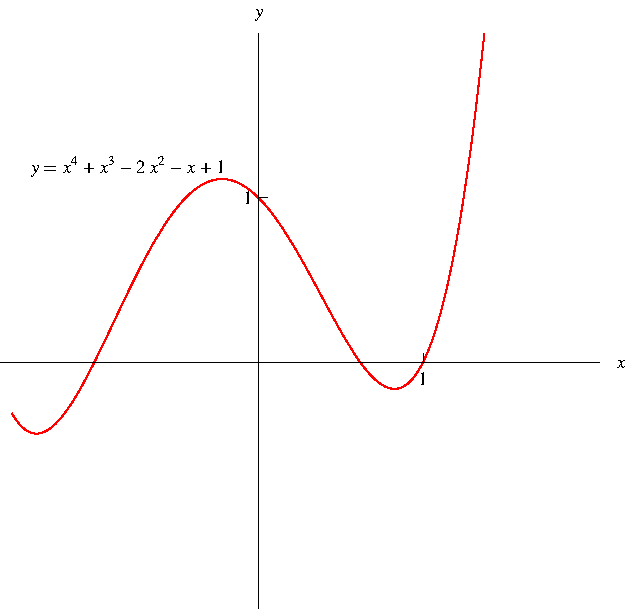
\includegraphics[height=6cm]{precalculus/pictures/01-02-polyb.pdf}%

Quartic
}%
\only<handout:5| 5>{%
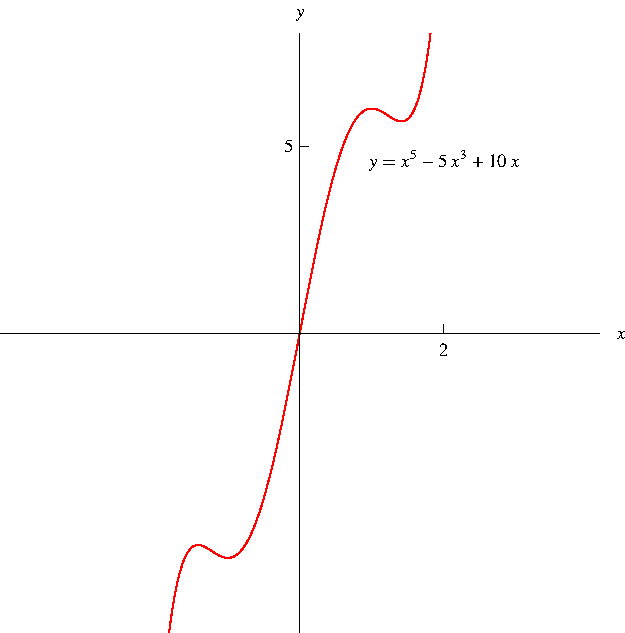
\includegraphics[height=6cm]{precalculus/pictures/01-02-polyc.pdf}%

Quintic
}
\end{frame}
% end module polynomials

\subsection{Power Functions}
%Old Version from Greg. Greg, this slide is changed substantially, please take a look.
%% begin module power-functions-def
%\begin{frame}
%\frametitle{Power Functions}
%\begin{definition}[Power Function]
%A power function is a function of the form
%\[
%f(x) = x^a,
%\]
%where $a$ is a fixed real number.
%\end{definition}
%\uncover<2->{
%If $a$ is a positive integer like $1, 2, 3, \ldots$ then $x^a$ is a polynomial.

%\only<handout:-2| -2>{%
%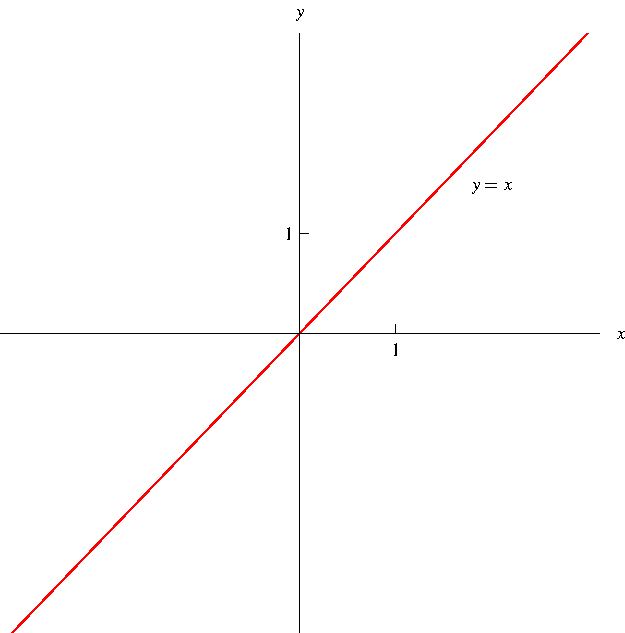
\includegraphics[height=4cm]{precalculus/pictures/01-02-x.pdf}%
%}%
%\only<handout:3| 3>{%
%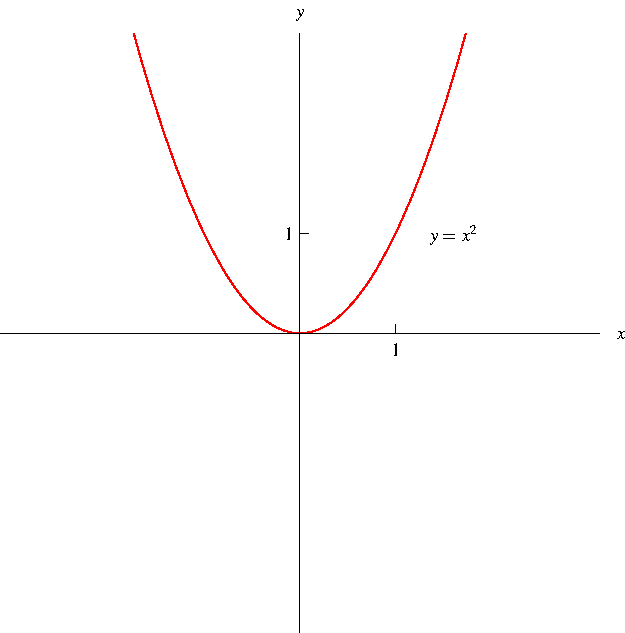
\includegraphics[height=4cm]{precalculus/pictures/01-02-xsquared.pdf}%
%}%
%\only<handout:4| 4>{%
%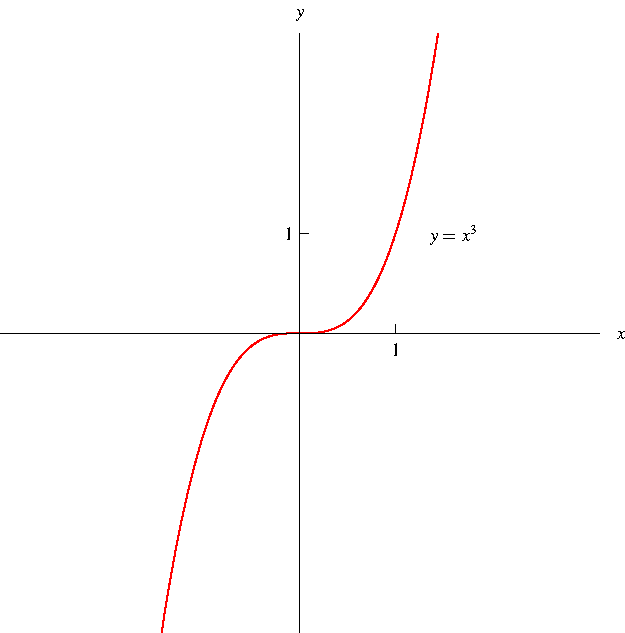
\includegraphics[height=4cm]{precalculus/pictures/01-02-xcubed.pdf}%
%}%
%\only<handout:5| 5>{%
%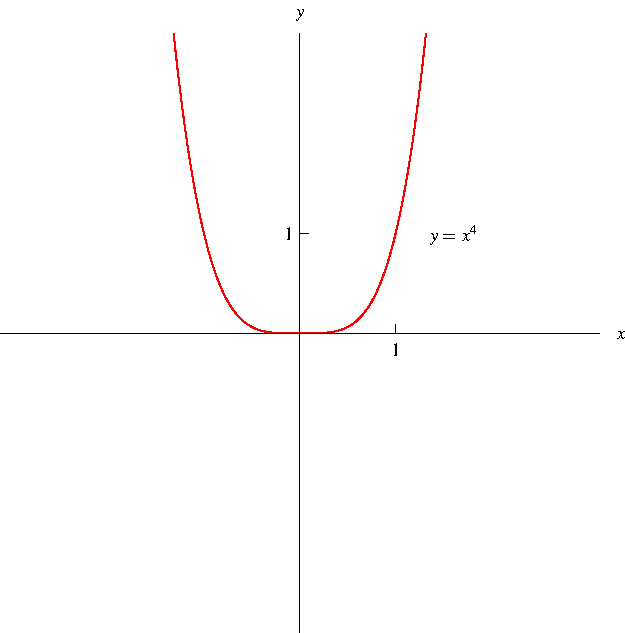
\includegraphics[height=4cm]{precalculus/pictures/01-02-xfourth.pdf}%
%}%
%\only<handout:6| 6>{%
%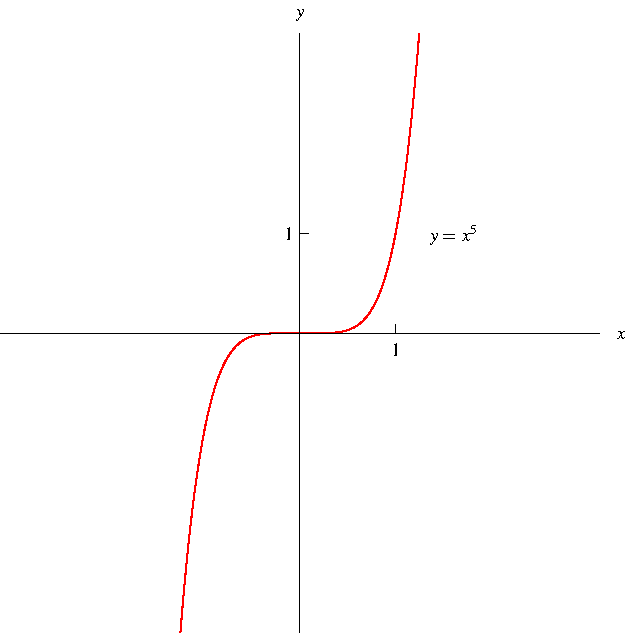
\includegraphics[height=4cm]{precalculus/pictures/01-02-xfifth.pdf}
%}%
%}%
%\end{frame}
%% end module power-functions-def

% begin module power-functions-def
\begin{frame}[t]
\frametitle{Power Functions}
\begin{definition}[Power Function]
Let $x>0$, $a$ - arbitrary real number. The power function is defined as
\[
f(x) \uncover<4->{\alert<handout: 0| 4>{=e^{a\ln x} } }= \alert<2>{x}^{\alert<3>{a}} \quad .
\]
\uncover<2->{$x$ = \alert<2>{base}. } \uncover<3->{$a$ = \alert<3>{exponent} or \alert<3>{power}. }
\uncover<4->{\alert<handout:0| 4>{First equality = one of ways to define for non-integer $a$ (we study $\ln x$, $e^x$ later). } }
\end{definition}
\begin{tabular}{l}
\uncover<5->{
If $a$ - positive integer ($1, 2, 3, \ldots$) \\
then $x^a$ = polynomial function.
}\\
\uncover<5->{
$x^{n}    =\underbrace{x\dots x }_{n~\mathrm{times}}$ when $n$-integer. \\
$\alert<12>{(x^{a})^b}=\uncover<13->{\alert<13>{x^{ab}}}$  \\
$\alert<14>{(xy)^b}   =\uncover<15->{\alert<15>{x^by^b}}$\\
$\alert<16>{x^{a+b}}  =\uncover<17->{\alert<17>{x^ax^b }}$ \\
$\alert<18>{x^{-a}}   =\uncover<19->{\alert<19>{\frac{1}{x^a}}}$\\
~\\~\\~\\~\\~\\~\\~\\
}
\end{tabular}
\uncover<6->{
\psset{xunit=0.38cm,yunit=0.38cm}
\begin{pspicture}(-5,-5)(5,5)
\psaxes[labels=none]{<->}(0,0)(-5,-5)(5,5)
\tiny
\rput[r](0,5){\tiny{$y$}}
\rput[l](5,0){\tiny{$x$}}
\only<7>{
\psplot[linecolor=red]{-5}{5}{ x 1 exp }
\rput( 3, 1){$y=x^{\phantom{1}}$}
} %only
\only<8>{
\psplot[linecolor=red]{-2.23}{2.23}{ x 2 exp }
\rput( 3, 1){$y=x^2$}
}
\only<9>{
\psplot[linecolor=red]{-1.7}{1.7}{ x 3 exp }
\rput( 3, 1){$y=x^3$}
}
\only<10>{
\psplot[linecolor=red]{-1.49}{1.49}{ x 4 exp }
\rput( 3, 1){$y=x^4$}
}
\only<11->{
\psplot[linecolor=red]{-1.37}{1.37}{ x 5 exp }
\rput( 3, 1){$y=x^5$}
}
\end{pspicture}
%\only<handout:-2| -2>{%
%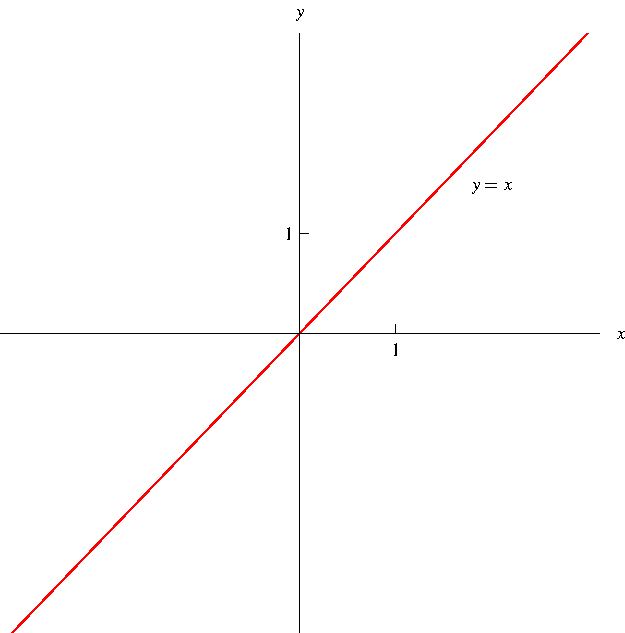
\includegraphics[height=4cm]{precalculus/pictures/01-02-x.pdf}%
%}%
%\only<handout:3| 3>{%
%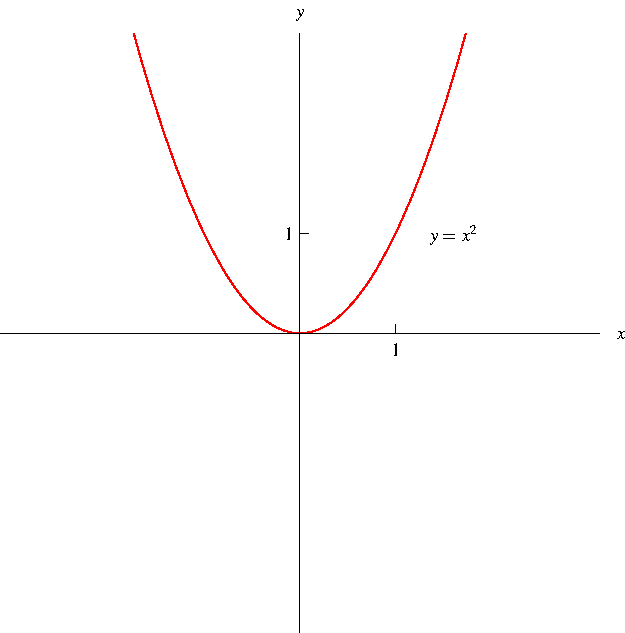
\includegraphics[height=4cm]{precalculus/pictures/01-02-xsquared.pdf}%
%}%
%\only<handout:4| 4>{%
%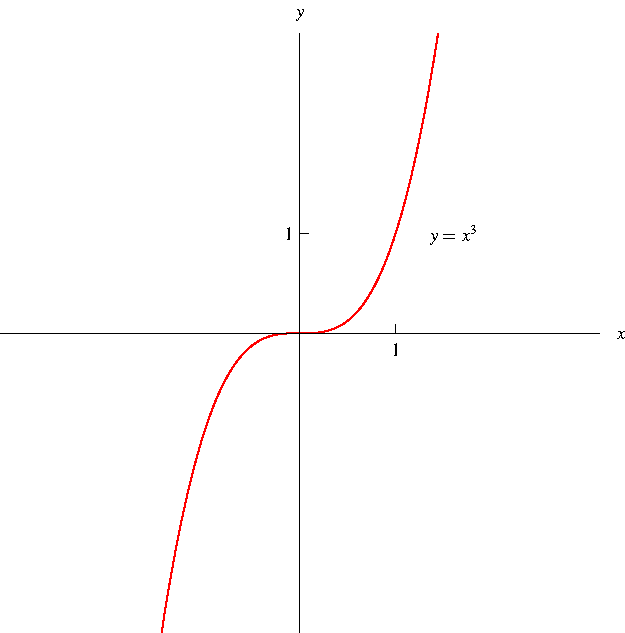
\includegraphics[height=4cm]{precalculus/pictures/01-02-xcubed.pdf}%
%}%
%\only<handout:5| 5>{%
%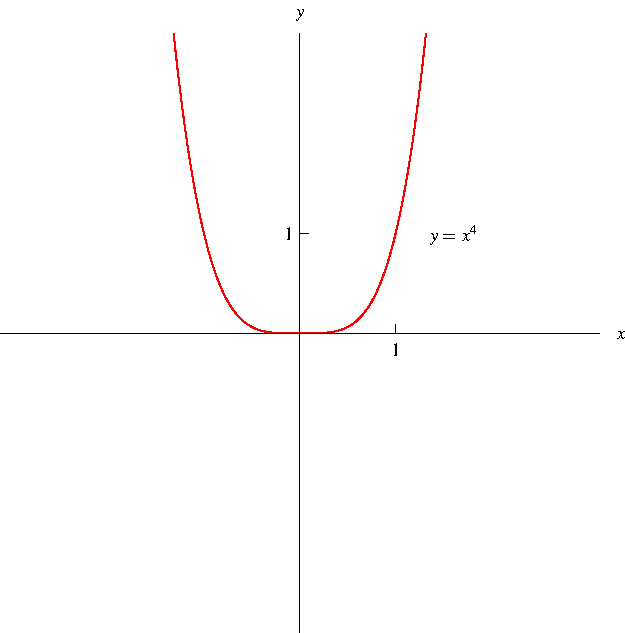
\includegraphics[height=4cm]{precalculus/pictures/01-02-xfourth.pdf}%
%}%
%\only<handout:6| 6>{%
%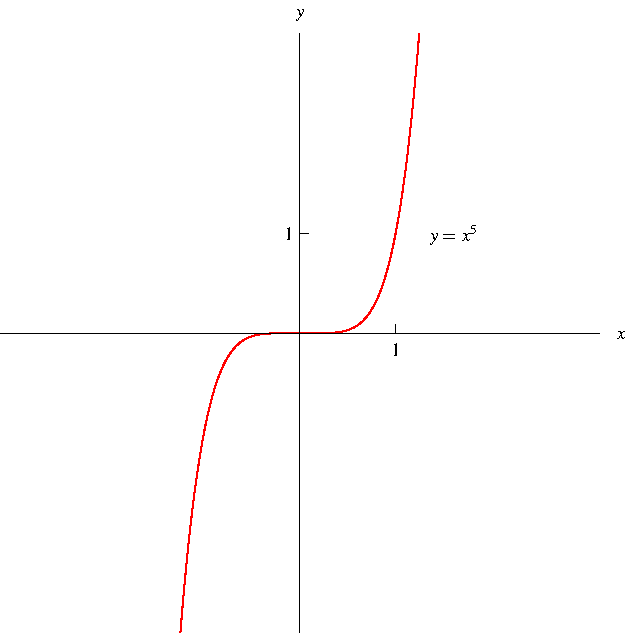
\includegraphics[height=4cm]{precalculus/pictures/01-02-xfifth.pdf}
%}%
}
\end{frame}
% end module power-functions-def

% begin module root-functions
\begin{frame}
\begin{itemize}
\item<1->  If $n$ is a positive integer, the function $f(x) = x^{\frac{1}{n}} = \sqrt[n]{x}$ is called a root function.
\item<2->  When $n = 2$, it is the square root function $f(x) = \sqrt{x}$.
\item<3->  The square root is not defined for negative numbers, so its domain is $[0, \infty)$.
\item<4->  Its graph is the top half of the parabola $x = y^2$.
\item<5->  The graph of the cube root function $f(x) = \sqrt[3]{x}$ is similar to that of the square root, but it is defined everywhere.
\end{itemize}
\begin{tabular}{cc}
\uncover<2->{%
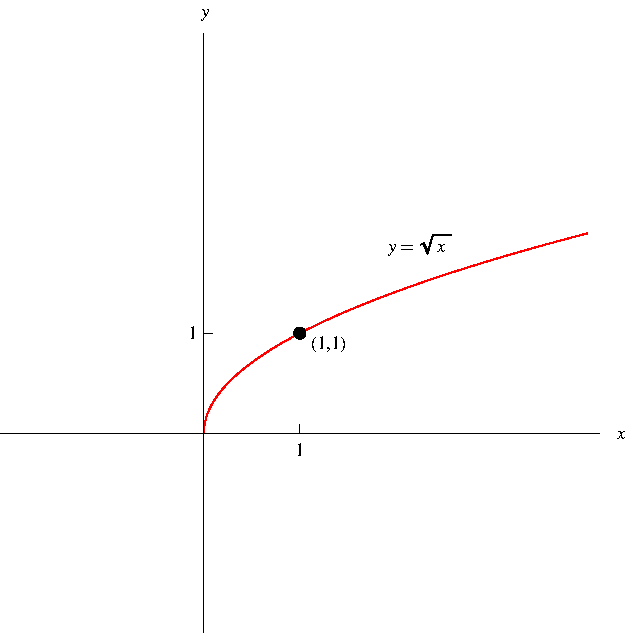
\includegraphics[height=3.5cm]{precalculus/pictures/01-02-sqrtx.pdf}%
}%
&%
\uncover<5->{%
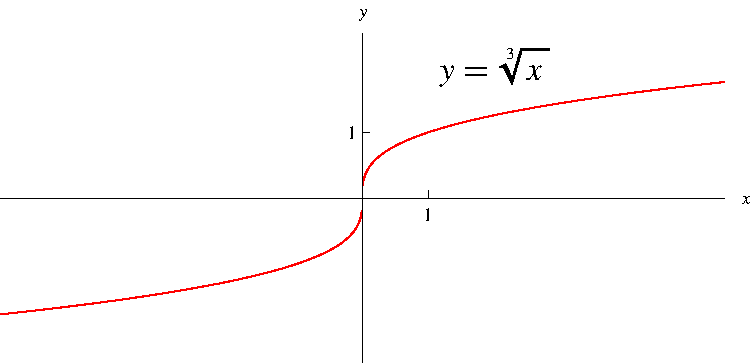
\includegraphics[height=3.5cm]{precalculus/pictures/cube-root.pdf}%
}%
\end{tabular}
\end{frame}
% end module root-functions

% begin module reciprocal-function
\begin{frame}
$f(x) = x^{-1} = \frac{1}{x}$ is called the reciprocal function.  Its graph has equation $y = \frac{1}{x}$, or $xy = 1$, and is an hyperbola with the coordinate axes as its asymptotes.
%\begin{center}%center does not work with well with pstricks and pgflayout.
\hfil\hfil\psset{xunit=0.6cm, yunit=0.6cm}
\begin{pspicture}(-5, -5)(5,5)
\psframe*[linecolor=white](-5,-5)(5,5)
\psaxes[ticks=none, labels=none]{<->}(0,0)(-5,-5)(5,5)\tiny
%Function formula: (1)/(x)
\rput(1,3){$y=\frac 1 x$}
\psplot[linecolor=red, plotpoints=1000]{0.2}{5}{1 x div } %Function formula: (1)/(x)
\rput(1,3){$y=\frac 1 x$}
\psplot[linecolor=red, plotpoints=1000]{-5}{-0.2}{1 x div }
\fcLabels{4.5}{4.5}
\end{pspicture}
%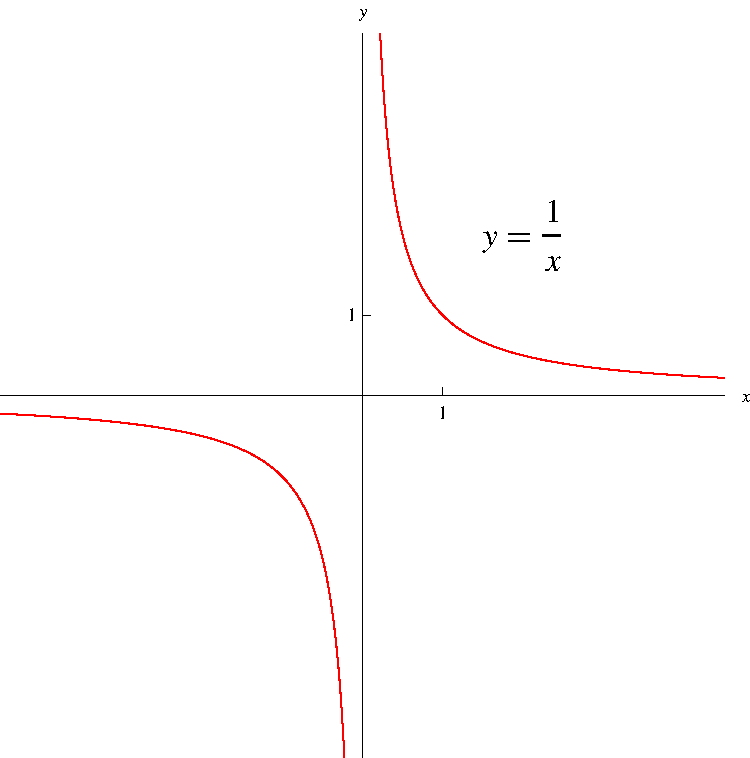
\includegraphics[height=5cm]{precalculus/pictures/reciprocal-function.pdf}%
%\end{center}
\end{frame}
% end module reciprocal-function

\subsection{Rational Functions}
% begin module rational-functions
\begin{frame}
\frametitle{Rational Functions}
\begin{definition}[Rational Function]
A rational function is a quotient of two polynomials; that is, a function of the form
\[
f(x) = \frac{g(x)}{h(x)},
\]
where $g$ and $h$ are polynomials.
\end{definition}
\begin{columns}[c]
\column{.4\textwidth}
\uncover<2->{
\psset{xunit=0.4cm, yunit=0.4cm}
\begin{pspicture}(-5, -5)(5,5) 
\psframe*[linecolor=white](-5,-5)(5,5) 
\psaxes[ticks=none, labels=none]{<->}(0,0)(-4.5,-4.5)(4.5,4.5)\tiny
%Function formula: \frac{x}{(x)^{2}-1} 
\rput(2.5,-3){$y=\frac{x}{x^{2}-1}$} 
\psplot[linecolor=red, plotpoints=1000]{1.11727}{4.5}{x -1 x 2 exp add div } %Function formula: \frac{x}{(x)^{2}-1} 
\psplot[linecolor=red, plotpoints=1000]{-0.895043}{0.895043}{x -1 x 2 exp add div } %Function formula: \frac{x}{(x)^{2}-1} 
\psplot[linecolor=red, plotpoints=1000]{-4.5}{-1.11727}{x -1 x 2 exp add div }
\psLabels{4.5}{4.5}
\end{pspicture} 
%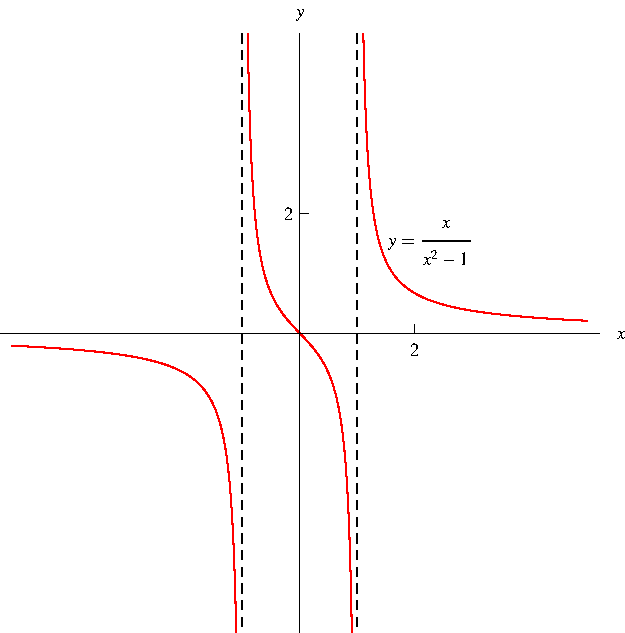
\includegraphics[height=4cm]{precalculus/pictures/01-02-rational.pdf}%
}
\column{.6\textwidth}
\uncover<2->{
\begin{example}[$x/(x^2-1)$]
The function
\[
f(x) = \frac{x}{x^2-1}
\]
is a rational function.
\end{example}
}
\end{columns}
\end{frame}
% end module rational-functions

\subsection{Algebraic Functions}
%Old Version from Greg. Greg, this slide is changed substantially, please take a look.
%% begin module algebraic-functions
%\begin{frame}
%\frametitle{Algebraic Functions}
%\begin{definition}[Algebraic Function]
%An algebraic function is a function that can be constructed using algebraic operations (such as addition, subtraction, multiplication, division, and taking roots) starting from polynomials.
%\end{definition}
%\uncover<2->{
%Algebraic functions can look pretty funny.
%\begin{tabular}{ccc}
%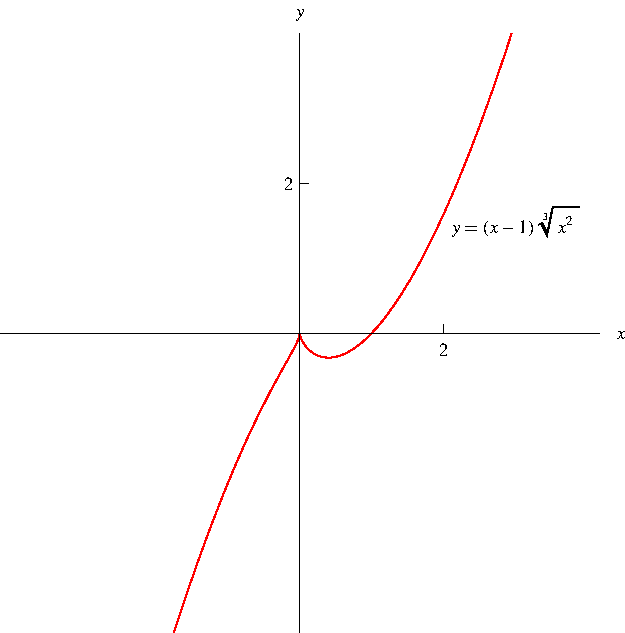
\includegraphics[height=3.8cm]{precalculus/pictures/01-02-algebraic1.pdf}&%
%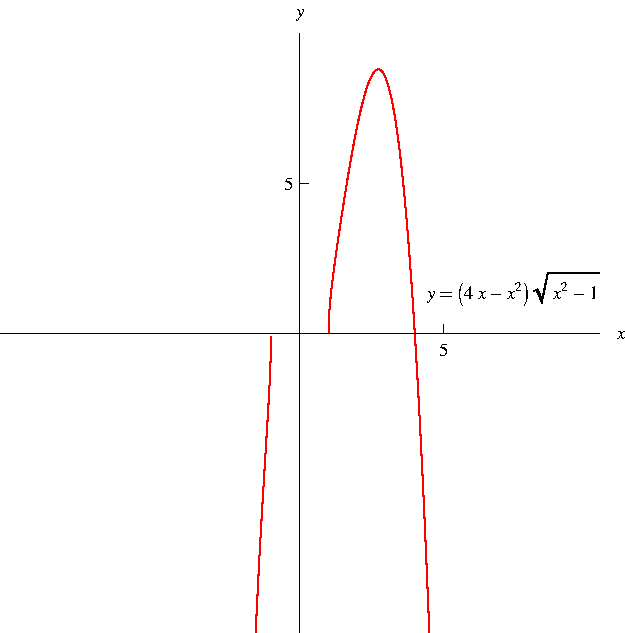
\includegraphics[height=3.8cm]{precalculus/pictures/01-02-algebraic2.pdf}&%
%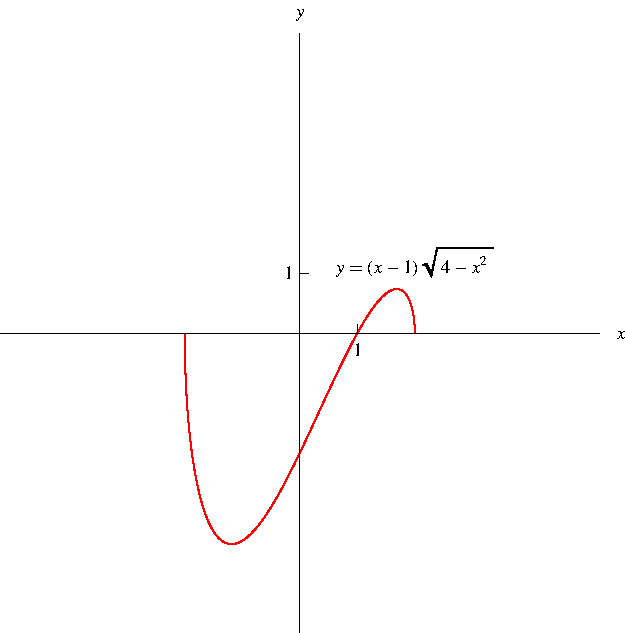
\includegraphics[height=3.8cm]{precalculus/pictures/01-02-algebraic3.pdf}%
%\end{tabular}
%}
%\end{frame}
%% end module algebraic-functions


% begin module algebraic-functions
\begin{frame}
\frametitle{Algebraic Functions}
\begin{definition}[Algebraic Function]
A function in $x$ that can be constructed using $x$, constants, and finitely many of the operations $+, -, *, /,$ and $\sqrt[n]{~}$ is an algebraic function.

\uncover<2->{{\footnotesize Outside of Calculus I: function $f(x)$ = algebraic if it satisfies a polynomial equation with polynomial coefficients, i.e., $a_0(x) +a_1(x)f(x)+\dots +a_n(x) \left(f(x)\right)^n=0$ for some polynomials  $a_i(x)$.}}
\end{definition}
\uncover<3->{
Examples.

\begin{tabular}{ccc}
\psset{xunit=0.3cm, yunit=0.3cm}
\begin{pspicture}(-5, -5)(5,5)
\tiny\psframe*[linecolor=white](-5,-5)(5,5)
\psaxes[ticks=none, labels=none]{<->}(0,0)(-4.5,-4.5)(4.5,4.5)\tiny
%Function formula: - ((- (x))^{5/3})- ((- (x))^{2/3})
\psplot[linecolor=red, plotpoints=1000]{-2}{-0.001}{x -1 mul 0.666667 exp -1 mul x -1 mul 1.66667 exp -1 mul add } %Function formula: (x)^{5/3}- ((x)^{2/3})
\rput[t](1,-5){$y=(x-1)\sqrt[3]{x^2}$}
\psplot[linecolor=red, plotpoints=1000]{0.001}{3}{x 0.666667 exp -1 mul x 1.66667 exp add }
\fcLabels{4.5}{4.5}
\end{pspicture}
%\includegraphics[height=3.8cm]{precalculus/pictures/01-02-algebraic1.pdf}
&%
\psset{xunit=0.3cm, yunit=0.3cm}
\begin{pspicture}(-5, -5)(5,5)
\tiny\psframe*[linecolor=white](-5,-5)(5,5)
\psaxes[ticks=none, labels=none]{<->}(0,0)(-4.5,-4.5)(4.5,4.5)\tiny
\psplot[linecolor=red, plotpoints=1000]{1}{5}{-1 x 2 exp add 0.5 exp x 2 exp mul -0.2 mul -1 x 2 exp add 0.5 exp x mul 0.8 mul add } %Function formula: 4/5 ((x) (((x)^{2}-1)^{1/2}))-1/5 (((x)^{2}) (((x)^{2}-1)^{1/2}))
\rput[t](1,-5){$y=\frac15(4x-x^2)\sqrt{x^2-1}$}
\psplot[linecolor=red, plotpoints=1000]{-2}{-1}{-1 x 2 exp add 0.5 exp x 2 exp mul -0.2 mul -1 x 2 exp add 0.5 exp x mul 0.8 mul add }
\fcLabels{4.5}{4.5}
\end{pspicture}
%\includegraphics[height=3.8cm]{precalculus/pictures/01-02-algebraic2.pdf}
&%
\psset{xunit=0.3cm, yunit=0.3cm}
\begin{pspicture}(-5, -5)(5,5)
\tiny\psframe*[linecolor=white](-5,-5)(5,5)
\psaxes[ticks=none, labels=none]{<->}(0,0)(-4.5,-4.5)(4.5,4.5)\tiny
%Function formula: - ((4- ((x)^{2}))^{1/2})+(x) ((4- ((x)^{2}))^{1/2})
\rput[t](1,-5){$y=(x-1)\sqrt{4-x^2}$}
\psplot[linecolor=red, plotpoints=1000]{-2}{2}{x 2 exp -1 mul 4 add 0.5 exp x mul x 2 exp -1 mul 4 add 0.5 exp -1 mul add }
\fcLabels{4.5}{4.5}
\end{pspicture}
%\includegraphics[height=3.8cm]{precalculus/pictures/01-02-algebraic3.pdf}
%
\end{tabular}
}
\end{frame}
% end module algebraic-functions

\subsection{Transcendental Functions}
% begin module transcendental-functions
\begin{frame}
\frametitle{Transcendental Functions}
Transcendental functions include many classes of functions.
\begin{itemize}
\item<2->  Trigonometric functions such as $\cos x, \sin x, \tan x,$ etc.
\item<3->  Exponential functions such as $2^x, \left( \frac{1}{2}\right)^x, 5^x, e^x$, etc.
\item<4->  The logarithm function $\ln x$.
\item<5->  And many more.
\item<6-> Outside of Calculus I: by definition, a function is transcendental if it is not algebraic, i.e., if it satisfies no polynomial equation.
\end{itemize}
\end{frame}
% end module transcendental-functions 

\subsection{Miscellaneous}
% begin module greatest-integer-function
\begin{frame}
\begin{definition}[Greatest Integer Function]
The greatest integer function $[[x]]$ is defined by $[[x]] =$ the largest integer that is less than or equal to $x$.
\end{definition}
\begin{columns}[c]
\column{.5\textwidth}
\ \includegraphics[height=4.5cm]{continuity/pictures/02-05-ex2d.pdf}%
\column{.5\textwidth}
\begin{align*}
\uncover<2->{%
\alert<handout:0| 2-3>{%
[[%
4%
]]%
}}%
& \uncover<2->{%
\alert<handout:0| 2-3>{%
 = \uncover<handout:0| 3->{%
 4%
}}}\\%
\uncover<2->{%
\alert<handout:0| 4-5>{%
[[%
4.8%
]]%
}}%
& \uncover<2->{%
\alert<handout:0| 4-5>{%
 = \uncover<handout:0| 5->{%
 4%
}}}\\%
\uncover<2->{%
\alert<handout:0| 6-7>{%
[[%
\pi%
]]%
}}%
& \uncover<2->{%
\alert<handout:0| 6-7>{%
 = \uncover<handout:0| 7->{%
 3%
}}}\\%
\uncover<2->{%
\alert<handout:0| 8-9>{%
[[%
\sqrt{2}%
]]%
}}%
& \uncover<2->{%
\alert<handout:0| 8-9>{%
 = \uncover<handout:0| 9->{%
 1%
}}}\\%
\uncover<2->{%
\alert<handout:0| 10-11>{%
\left[\left[%
-\frac{1}{2}%
\right]\right]%
}}%
& \uncover<2->{%
\alert<handout:0| 10-11>{%
 = \uncover<handout:0| 11->{%
-1%
}}}%
\end{align*}
\end{columns}
\end{frame}
% end module greatest-integer-function

\section{New Functions from Old Functions}
% begin module combinations-functions
\begin{frame}
\frametitle{Combinations of Functions}
Two functions $f$ and $g$ can be combined to form new functions $f+g$, $f-g$, $f\cdot g$, and $\frac{f}{g}$:
\[
\begin{array}{rcll|l}
\uncover<2->{\alertNoH{3} {(f+g)(x)}} &\uncover<2->{\alertNoH{3}{=} }&\uncover<3->{ \alertNoH{3}{f(x) + g(x)}}\\
\uncover<2->{\alertNoH{4,5}{(f-g)(x)}}&\uncover<2->{\alertNoH{4,5}{=}}&\fcAnswer{5}{ f(x)-g(x)} \\
\uncover<2->{\alertNoH{6,7} {(f\cdot g)(x) }}&\uncover<2->{\alertNoH{6,7}{=}}& \fcAnswer{7}{f(x) \cdot g(x)}\\
\uncover<2->{\alertNoH{8,9}{\left(\frac{f}{g}\right) (x)}}& \uncover<2->{\alertNoH{8,9}{=}}& \fcAnswer{9}{ \frac{f(x)}{\alertNoH{10}{g(x)}}}\uncover<9->{ && \alertNoH{10,21}{\text{for } g(x)\neq 0}\quad .}
\end{array}
\]
\uncover<11->{Let $\text{Dom}(f)$ denote the domain of $f$.} \uncover<13->{\alertNoH{14,15}{The function $f+g$ is defined only if both $f$ and $g$ are defined, and similarly for the others. }} \uncover<14->{\alertNoH{14}{Therefore}} 
\[
\begin{array}{@{}rcll|l}
\uncover<12->{\alertNoH{14,15}{\text{Dom}(f+g)}}&\uncover<12->{\alertNoH{13,14,15}=}&\fcAnswerUncover{12}{15}{ \text{Dom}(f)\alertNoH{16}{ \cap} \text{Dom}(g) } \uncover<15->{&&\alertNoH{16}{ \cap\text{ stands for} } } \\
\uncover<12->{\alertNoH{17,18}{\text{Dom}(f-g)}}&\uncover<12->{\alertNoH{17,18}{=}}&\fcAnswerUncover{12}{18}{ \text{Dom}(f)\cap \text{Dom}(g) } \uncover<15->{&&\alertNoH{16}{\text{set intersection}} }\\
\uncover<12->{\alertNoH{17,18}{ \text{Dom}(f\cdot g)}} &\uncover<12->{ \alertNoH{17,18}{=}} &\fcAnswerUncover{12}{18} { \text{Dom}(f)\cap \text{Dom}(g)}\\
\uncover<12->{\alertNoH{19,20}{ \text{Dom}\left(\frac{f}{g}\right)}} &\uncover<12->{\alertNoH{19,20}{=}}& \fcAnswerUncover{12}{20}{ \text{Dom}(f)\cap \text{Dom}(g) \cap\alertNoH{21}{ \alertNoH{22}{\{} x\alertNoH{23}{ \textbf{|} }\alertNoH{24}{ g(x)\neq 0} \alertNoH{22}{ \}}} } \uncover<21->{ &&\alertNoH{21}{ \begin{array}{@{}l}\text{right expr.} \\ \text{stands for \alertNoH{22}{set} } \\ \alertNoH{23}{\text{where }} \alertNoH{24}{g(x)\neq 0}\end{array}}} \\
\end{array}
\]

\end{frame}

% end module combinations-functions

% begin module composition-functions
\begin{frame}
\begin{definition}[Composition of $f$ and $g$]
If $f$ and $g$ are two functions, then the composition of $f$ and $g$ is written $f\circ g$ and is defined by the formula
\[
(f\circ g)(x) = f(g(x)).
\]
\end{definition}

Imagine $f$ and $g$ as machines taking some input and producing some output. Then $f\circ g$ corresponds to attaching both machines end-to-end so that the output of $g$ becomes the input of $f$.
\includegraphics[height=2cm]{precalculus/pictures/01-03-machines.pdf}%

\uncover<2->{
The domain of $f\circ g$ is the set of all numbers $x$ in the domain of $g$ such that $g(x)$ is in the domain of $f$.  If the domain of $f$ is $A$ and the domain of $g$ is $B$, we write this as
\[
\{ x\in B |\ g(x) \in A\} .
\]
}
\end{frame}
% end module composition-functions

% begin module composition-example
\begin{frame}
\begin{example}
Find $\alertNoH{2}{f\circ g},\alertNoH{14}{g\circ f}, \alertNoH{27}{g\circ g}$ and their domains, where \alertNoH{10,16}{$\alertNoH{5}{ f(} \alertNoH{6}{ x} \alertNoH{5}{) =}\only<handout:0|5> {\color{red}} \sqrt{\only<handout:0|5>{\color{black}} \alertNoH{6}{x}}$} and \alertNoH{4,29}{$\alertNoH{17,30}{ g(}\alertNoH{18,31}{ x} \alertNoH{17,30}{) = }\only<handout:0|17,30>{\color{red}} \sqrt{3 - \only<handout:0|17,30>{ \color{black}} \alertNoH{18,31}{x} }$}.

$
\begin{array}{rclll}
\only<handout:1|1-26>{%
\uncover<2->{\alertNoH{3}{ (\alertNoH{2}{f\circ g})(x)}} &\uncover<3->{ \alertNoH{3}{ =}} & \uncover<3->{\alertNoH{3}{ f(\alertNoH{4}{g(x)})}} \uncover<4->{ =\only<handout:0|5>{\color{red}} f\left( \only<handout:0|5>{ \color{black}}   \alertNoH{4,6}{\sqrt{3 - x}} \only<handout:0|5>{\color{red}} \right)} \uncover<5->{ = \only<handout:0|5>{ \color{red}}  \alertNoH{7}{\sqrt{ \only<handout:0|5>{ \color{black}} \alertNoH{6}{\sqrt{3-x}}}}} \uncover<7->{  \alertNoH{7}{= \sqrt[4]{\alertNoH{7,9}{ 3-x} }}}\\
\uncover<8->{\text{Domain: }}\\
\uncover<9->{\alertNoH{9}{\alertNoH{10}{3}-x}&\alertNoH{9}{\geq} & \alertNoH{9}{0}} \\
\uncover<10->{\alertNoH{11}{-}x&\alertNoH{11}{\geq} & \alertNoH{10}{ \alertNoH{11}{-} 3}}\\
\uncover<11->{\alertNoH{13}{x}&\alertNoH{11,13}{\leq}&\alertNoH{13}{ 3} }\\
\uncover<12->{\alertNoH{12,13}{x} &\alertNoH{12,13}{\in}& \fcAnswer{13}{(-\infty , 3].}}\\
\uncover<14->{\alertNoH{15}{ (\alertNoH{14}{g\circ f})(x)}}& \uncover<15->{ \alertNoH{15}{=} } & \uncover<15->{ \alertNoH{15}{ g(\alertNoH{16}{ f(x)})}}
\uncover<16->{ = \alertNoH{17}{g(}\alertNoH{16,18}{\sqrt{x}}\alertNoH{17}{)}} \uncover<17->{ = \only<handout:0|17>{\color{red}}  \sqrt{\alertNoH{21}{ 3 - \only<handout:0|17>{ \color{black}} \alertNoH{18}{\sqrt{\alertNoH{20}{x}} }} }}\\
\uncover<19->{\text{Domain}:}\\
\uncover<20->{\alertNoH{20,26}{x}&\alertNoH{20,26}{\geq} & \alertNoH{20,26}{0} }\\
\uncover<21->{\alertNoH{21}{\alertNoH{22}{ 3} - \sqrt{x}}& \alertNoH{21}{ \geq } & \alertNoH{21}{ 0} }\\
\uncover<22->{ \alertNoH{23}{-} \sqrt{x} &\alertNoH{23}{\geq }& \alertNoH{22}{ \alertNoH{23}{-}3 }}\\
\uncover<23->{\sqrt{x}&\alertNoH{23}{ \leq} & 3} \\
\uncover<24->{\alertNoH{26}{ x}& \alertNoH{26}{ \alertNoH{0}{\leq}} &\alertNoH{26}{ 9}}\\
\uncover<25->{ \alertNoH{25,26}{x}&\alertNoH{25,26}{\in}& \fcAnswer{26}{[0,9]}} \\
}%only<handout:1|1->
\only<handout:2|27->{%
\uncover<27->{\alertNoH{28}{ (\alertNoH{27}{g\circ g})(x)}} & \uncover<28->{ \alertNoH{28} {=} } & \uncover<28->{\alertNoH{28}{ g( \alertNoH{29 }{ g(x)})}} \uncover<29->{ = \only<handout:0|30>{\color{red}}  g \left( \only<handout:0|30>{ \color{black}} \alertNoH{29}{\sqrt{3 - x}}  \only<handout:0|30>{\color{red}} \right)}  \uncover<30->{ \only<handout:0|30>{\color{red}} = \sqrt{\alertNoH{36}{ 3 - \only<handout:0|30>{\color{black}}\alertNoH{31}{\sqrt{\alertNoH{33}{3-x} } }}}}\\
\uncover<32->{\text{Domain}:}\\
\uncover<33->{\alertNoH{33}{\alertNoH{34} {3}-x} & \alertNoH{33}{\geq} &\alertNoH{33}{ 0}}\\
\uncover<34->{\alertNoH{35}{-}x&\alertNoH{35}{\geq} & \alertNoH{34}{ \alertNoH{35}{ - } 3}}\\
\uncover<35->{\alertNoH{43}{x}&\alertNoH{35,43}{\leq} &\alertNoH{43}{ 3}}\\
\uncover<36->{\alertNoH{36}{\alertNoH{37}{3}-\sqrt{3-x}}&\alertNoH{36}{\geq }&\alertNoH{36}{ 0}} \\
\uncover<37->{\alertNoH{38}{-}\sqrt{3-x}&\alertNoH{38}{\geq}& \alertNoH{37}{\alertNoH{38}{-} 3}}\\
\uncover<38->{\sqrt{3-x}&\alertNoH{38}{\leq}& 3} \\
\uncover<39->{\alertNoH{40}{3}-x&\alertNoH{0}{\leq} &\alertNoH{40}{ 9}}\\
\uncover<40->{\alertNoH{41}{-}x&\alertNoH{41}{\leq}& \alertNoH{40}{6}}\\
\uncover<41->{\alertNoH{43}{x}&\alertNoH{41,43}{\geq}& \alertNoH{43}{ \alertNoH{41}{-}6} }\\
\uncover<42->{\alertNoH{42,43}{x}&\alertNoH{42,43}{\in}& \fcAnswer{43}{[-6 , 3].}}
}%only<handout:2|>
\end{array}
$

%\column{.2\textwidth}
%\begin{eqnarray*}
%& & f\circ f  \\
%& & \uncover<2->{(f\circ f)(x)}\\
%& \uncover<3->{ = } & \uncover<3->{f(\alertNoH{ 4}{f(x)})}\\
%& \uncover<4->{ = } & \uncover<4->{\alertNoH{ 5}{f(}\alertNoH{ 4-5}{\sqrt{x}}\alertNoH{ 5}{)}}\\
%& \uncover<5->{ = } & \uncover<5->{\alertNoH{ 5}{\sqrt{\sqrt{x}}}}\\
%& \uncover<6->{ = } & \uncover<6->{\alertNoH{ 5}{\sqrt[4]{x}}}\\
%\end{eqnarray*}
\end{example}

\vskip 10cm
\end{frame}
% end module composition-example

\begin{frame}
\vskip -0.2cm
\begin{example}
Give simplified f-las for $f\circ g$, $f\circ f$, $g\circ f$, $g\circ g$. \alertNoH{2,3,4,5,21,22,31,32}{Find the implied domains.}
$
\begin{array}{@{}r@{}c@{}l@{}l|l}
\displaystyle \alertNoH{26}{ \alertNoH{8,27}{f(} \alertNoH{9,28}{x} \alertNoH{8,27}{)} }& \alertNoH{26}{=} &\displaystyle  \alertNoH{26}{ \only<handout:0|8,27>{\color{red}} \frac{2 \only<handout:0|8,27>{\color{black}} \alertNoH{9,28}{x} \only<handout:0|8,27>{\color{red}} -1}{\alertNoH{3,34}{\only<handout:0|8,27>{\color{black}}  \alertNoH{9,28}{x} \only<handout:0|8,27>{\color{red}} +2}}} && \uncover<2->{\alertNoH{2,3}{x \neq}  \fcAnswer{3}{-2}}\\
\displaystyle \alertNoH{7}{ g(x)}& \alertNoH{7}{=} &\displaystyle \alertNoH{7}{ \frac{2x+ 3}{\alertNoH{5,24}{5x-7}}} && \uncover<4->{\alertNoH{4,5,24}{x \neq}} \fcAnswer{5}{ \alertNoH{24}{\frac{7}{5}}}\\
\uncover<6->{% 
\displaystyle (f\circ g)(x)&\alertNoH{0}{=} &\displaystyle f(\alertNoH{7}{g(x)}) \uncover<7->{ = \only<handout:0|8>{\color{red}} f\left( \only<handout:0|8>{\color{black}} \alertNoH{7,9}{ \frac{2x+3}{ \alertNoH{24}{5x-7} }} \only<handout:0|8>{\color{red}}\right)\only<handout:0|8>{\color{black}}}
\uncover<8->{ = \only<handout:0|8>{\color{red}} \frac{ \alertNoH{10}{2} \only<handout:0|8>{\color{black}} \left( \alertNoH{9}{\frac{2x +3}{5x -7}} \right) \only<handout:0|8>{ \color{red}} -\alertNoH{11}{ 1} }{ \only<handout:0|8>{ \color{black}} \alertNoH{9}{\frac{2 x+3}{ 5x -7}} \only<handout:0|8>{\color{red}}+\alertNoH{12}{2 }}}
}%uncover<6-> 
\\
\uncover<10->{
&\alertNoH{0}{=}&\displaystyle \frac{ \frac{\alertNoH{10}{2} (2x+3)}{\alertNoH{13}{ 5x-7} }\alertNoH{14}{-} \alertNoH{11}{\frac{5x- 7}{ \alertNoH{13}{ 5x-7}}} }{\frac{2x+3}{ \alertNoH{13}{ 5x-7}}+ \alertNoH{12}{\frac{\alertNoH{15}{ 2( 5x-7) }}{\alertNoH{13}{ 5x-7}}}} \uncover<13->{= \frac{\frac{ \alertNoH{17}{ 4x} +\alertNoH{18}{6} \alertNoH{14 }{\alertNoH{17, 18}{-}(}\alertNoH{17}{5x}\alertNoH{18}{ - 7}\alertNoH{14}{)}}{\fcCancel{16}{ \alertNoH{13}{5 x-7} }}}{ \frac{\alertNoH{19}{2x} +\alertNoH{20}{3}+ (\alertNoH{15}{\alertNoH{19}{10x} \alertNoH{20}{ -14}}) }{\fcCancel{16}{ \alertNoH{13}{5x -7} }} }} \uncover<17->{= \frac{ \alertNoH{17}{-x} +\alertNoH{18}{ 13} }{\alertNoH{23}{ \alertNoH{19}{12x} \alertNoH{20}{-11}} } \uncover<21->{ && \alertNoH{21-24} {x\neq} \fcAnswer{22}{ \alertNoH{23}{ \frac{11}{12}} , \alertNoH{24}{\frac{7}{5}}}}}
}%uncover<10->
\\
\uncover<25->{
(f\circ f)(x)&\alertNoH{0}{=}& \displaystyle f(\alertNoH{26}{f(x)})\uncover<26->{ =\only<handout:0|27>{\color{red}} f\left(\only<handout:0|27>{\color{black}} \alertNoH{26,28}{ \frac{ 2x- 1}{\alertNoH{34}{x+2} }} \only<handout:0|27>{ \color{red}} \right) \only<handout:0|27>{\color{black}} } \uncover<27->{ = \alertNoH{29,30}{ \only<handout:0|27>{ \color{red}} \frac{  2  \only<handout:0|27>{ \color{black}} \left( \alertNoH{28}{\frac{ 2x- 1}{x+2}} \right)\only<handout:0|27>{\color{red}} -1 }{\only<handout:0|27>{\color{black}} \alertNoH{28}{\frac{ 2x- 1}{x+2}} \only<handout:0|27>{\color{red}}+2 }}
}}%uncover<25->
\\
\uncover<29->{ & \alertNoH{29,30}{=} &\displaystyle  \fcAnswer{30}{\frac{3 x-4}{ \alertNoH{33}{4 x+3} }} \uncover<31->{ && \alertNoH{31-34}{x\neq} \!\! \fcAnswer{32}{ \alertNoH{34}{-2}, \! \alertNoH{33}{ -\frac{3}{4}}} }
}%uncover<29->
 \\
\uncover<35->{ \alertNoH{35,36}{(g\circ f)(x)} &\alertNoH{35,36}{=}& \fcAnswer{36}{ \frac{7 x+4}{3 x-19}} && \alertNoH{35,36}{x\neq}  \fcAnswer{36}{ -2,\frac{19}{3}}} \\
\uncover<35->{\alertNoH{35,36}{ (g\circ g)(x)}&\alertNoH{35,36}{=} &\fcAnswer{36}{ \frac{19 x-15}{-25 x+64}} && \alertNoH{35,36}{ x \neq } \fcAnswer{36}{ \frac{7}{5},  \frac{64}{25} }}
\end{array}
$

\end{example}
\end{frame}
}

\lect{\semester}{Lecture 6}{6}{
\section{Composing Functions with Linear Transformations}
% begin module transformations-shifts
\begin{frame}
\frametitle{Transformations of Functions}
\begin{columns}[c]
\column{.5\textwidth}

\psset{xunit=1cm, yunit=1cm}
\begin{pspicture}(-0.5, -0.5)(4.7,4.7)%
\tiny%
\psframe*[linecolor=white](-5,-5)(5,5)%
\psaxes[ticks=none, labels=none]{<->}(0,0)(-0.5,-0.5)(5,4.5)%
\rput[t](5, -0.1){$x$}%
\rput[r](-0.1, 4.5){$y$}%
%\frac{1}{3} (3 x-6)^{3}-\frac{1}{3} (3 x-6)^{2}-\frac{1}{3} x+\frac{8}{3} 
\newcommand{\theFun}{3 x mul 6 sub dup dup mul mul 3 div 3 x mul 6 sub dup mul -3 div x -3 div 8 3 div add add add\space}%
\only<handout:0| -2>{%
\psplot[linecolor=red, plotpoints=1000]{1.65}{2.55}{\theFun}%
\rput[b] (2.55, 2.40654){\alert<-2>{$y=f(x)$}}%
}%
\only<handout:1| 3->{%
\psplot[linecolor=blue, plotpoints=1000]{1.65}{2.55}{\theFun}%
\rput[b] (2.55, 2.40654){$y=f(x)$}%
}%
\only<handout:0| 3>{%
\psplot[linecolor=red, plotpoints=1000]{1.65}{2.55}{\theFun 1.5 add }%
\rput[b](2.55, 3.90654){\alert<3>{$y=f(x)+c$}}%
}%
\only<handout:1| 4,5,22->{%
\psplot[linecolor=blue, plotpoints=1000]{1.65}{2.55}{\theFun 1.5 add }%
\rput[b](2.55, 3.90654){$y=f(x)+c$}%
}%
\only<handout:0| 4>{%
\psplot[linecolor=red, plotpoints=1000]{1.65}{2.55}{\theFun 1.5 sub}%
\rput[b](2.55, 0.906542){$y=f(x)-c$}%
}%
\only<handout:1| 5,22->{%
\psplot[linecolor=blue, plotpoints=1000]{1.65}{2.55}{\theFun 1.5 sub}%
\rput[b](2.55, 0.906542){$y=f(x)-c$}%
}%
\only<handout:0| 19>{%
\psplot[linecolor=red, plotpoints=1000]{3.15}{4.05}{1 dict begin /x x 1.5 sub def \theFun end}%
}%
\only<handout:1| 20,22->{%
\psplot[linecolor=blue, plotpoints=1000]{3.15}{4.05}{1 dict begin /x x 1.5 sub def \theFun end}%
\rput[b](4.05, 2.40654){$\alert<20>{y=f(x-c)}$}%
}%
\newcommand{\theAnimation}[6]{%
\uncover<handout:0|####1>{%
\fcXTickWithLabel{\curPt}{$x$}%
}%
\uncover<handout:0|####2>{%
\fcXTickWithLabel{\curPt 1.5 sub}{$x-c$}%
}%
\uncover<handout:0|####3>{%
\rput[l](! \curPt 1.5 sub 0.1 add 1 dict begin /x \curPt 1.5 sub def \theFun  end 2 div){$f(x-c)$}%
}%
\uncover<handout:0|####4>{%
\psline[linecolor=red, linewidth=2pt](! \curPt 1.5 sub 0)(! \curPt 1.5 sub 1 dict begin /x \curPt 1.5 sub def \theFun  end)%
}%
\uncover<handout:0|####5>{%
\rput[l](! \curPt 0.1 add 1 dict begin /x \curPt 1.5 sub def \theFun  end 2 div){$f(x-c)$}%
}%
\uncover<handout:0|####6>{%
\psline[linecolor=red, linewidth=2pt](! \curPt 0)(! \curPt 1 dict begin /x \curPt 1.5 sub def \theFun  end)%
}%
}%
\newcommand{\curPt}{3.3\space}%
\theAnimation{7-10}{8-10}{9-10}{9-19}{10}{10-19}%
\renewcommand{\curPt}{3.5\space}%
\theAnimation{11-14}{12-14}{13-14}{13-19}{14}{14-19}%
\renewcommand{\curPt}{3.8\space}%
\theAnimation{15-19}{16-19}{17-18}{17-19}{18}{18-19}%
%

\only<handout:0|21>{%
\psplot[linecolor=red, plotpoints=1000]{0.15}{1.05}{1 dict begin /x x 1.5 add def \theFun end}
\rput[b](1.05, 2.40654){\alert<6>{$y=f(x+c)$}}
}
\only<handout:1|22->{%
\psplot[linecolor=blue, plotpoints=1000]{0.15}{1.05}{1 dict begin /x x 1.5 add def \theFun end}
\rput[b](1.05, 2.40654){$y=f(x+c)$}
}
\end{pspicture}
%\ \only<handout:0| -2>{%
%\includegraphics[height=5cm]{precalculus/pictures/01-03-shifta.pdf}%
%}%
%\only<handout:0| 3>{%
%\includegraphics[height=5cm]{precalculus/pictures/01-03-shiftb.pdf}%
%}%
%\only<handout:0| 4>{%
%\includegraphics[height=5cm]{precalculus/pictures/01-03-shiftc.pdf}%
%}%
%\only<handout:0| 5>{%
%\includegraphics[height=5cm]{precalculus/pictures/01-03-shiftd.pdf}%
%}%
%\only<6>{%
%\includegraphics[height=5cm]{precalculus/pictures/01-03-shifte.pdf}%
%}%a
\column{.5\textwidth}
\begin{itemize}
\item What happens to the graph if we add/subtract a positive constant $c$ in the equation of a function $f$?
\item What happens if we add or subtract $c$ from $x$ before applying the function $f$?
\end{itemize}
\end{columns}

\uncover<2->{
\begin{tabular}{|l|l|}
\hline
\alertNoH{ 3}{$f(x)+c$} &%
\uncover<3->{\alertNoH{3,22}{Shift the graph of $f(x)$ $c$ units up.}} \\%
\alertNoH{ 4}{$f(x)-c$} &%
\uncover<4->{\alertNoH{4,22}{Shift the graph of $f(x)$ $c$ units down.}} \\%
\alertNoH{6}{$f(x-c)$} &%
\uncover<6->{\alertNoH{6,22}{Shift the graph of $f(x)$ \fcAnswerUncover{6}{20}{$c$ units right}.}} \\%
\alertNoH{21}{$f(x+c)$} &%
\uncover<21->{\alertNoH{21,22}{Shift the graph of $f(x)$ $c$ units left.}}\\%
\hline
\end{tabular}

}
\end{frame}
% end module transformations-shifts

% begin module transformations-shifts-example
\begin{frame}
\begin{example}
Draw a graph of the function $f(x) = x^2 + 6x + 10$.
\begin{columns}[c]
\column{.5\textwidth}

\psset{xunit=0.7cm, yunit=0.7cm}
\begin{pspicture}(-5.1, -0.6)(3.1,5.1)
\tiny
\fcAxesStandard{-5.03}{-0.5}{3}{5}
\rput[rt](-0.1,-0.1){$(0,0)$}
\fcFullDot{0}{0}
%Function formula: (-3+x)^{2}-9+6 (x)
\only<handout:0| 7>{
\rput(2.5,2){$y=x^2$}
\psplot[linecolor=red, plotpoints=1000]{-2.23607}{2.23607}{x 6 mul -9 x -3 add 2 exp add add } %Function formula: (x)^{2}+10+6 (x)
}
\only<handout:1| 8->{
\rput(2.5,2){\color{gray}$y=x^2$}
\psplot[linecolor=gray, plotpoints=1000]{-2.23607}{2.23607}{x 6 mul -9 x -3 add 2 exp add add } %Function formula: (x)^{2}+10+6 (x)
\rput[rt](-3.1,0.9){$(-3,1)$}
\psline{->}(0,0)(-3,1)
\fcFullDot{-3}{1}

\rput[b](-3,4.2){\alert<8->{$y=x^{2}+6x+10$}}
\psplot[linecolor=red, plotpoints=1000]{-5}{-1}{x 6 mul 10 x 2 exp add add }
}
\end{pspicture}

\column{.5\textwidth}
\uncover<2->{
Complete the square:
}
\begin{eqnarray*}
\uncover<3->{f(x)} & \uncover<3->{ = } & \uncover<3->{x^2 + 6x + 10} \\
& \uncover<4->{ = } & \uncover<4->{(x^2 + 6x \uncover<5->{\alert<handout:0| 5>{+ 9}}) + 10 \uncover<5->{\alert<handout:0| 5>{- 9}}} \\
 & \uncover<6->{ = } & \uncover<6->{(x + 3)^2 + 1} \\
\end{eqnarray*}
\end{columns}
\uncover<7-8>{}
\end{example}
\end{frame}
% end module transformations-shifts-example

% begin module transformations-magnifications
\begin{frame}
\begin{columns}[c]
\column{.5\textwidth}

\psset{xunit=0.7cm, yunit=0.7cm}
\begin{pspicture}(-4, -3.5)(4.5,5)
\tiny
\fcAxesStandard{-4}{-3.5}{4.5}{5}
%Function formula: 10/3+1/3 ((-3+3 (x))^{3})-1/3 ((-3+3 (x))^{2})-1/3 (x)
\only<handout:1| 1->{
\psplot[linecolor=red, plotpoints=1000]{1.65}{2.55}{x -0.333333 mul x 3 mul -6 add 2 exp -0.333333 mul x 3 mul -6 add 3 exp 0.333333 mul 2.66667 add add add }
\rput[b] (2.55, 2.40654){$y=f(x)$}
}
%\only<handout:0| 3->{
%\psplot[linecolor=blue, plotpoints=1000]{1.65}{2.55}{x -0.333333 mul x 3 mul %-6 add 2 exp -0.333333 mul x 3 mul -6 add 3 exp 0.333333 mul 2.66667 add add %add }
%\rput[b] (2.55, 2.40654){$y=f(x)$}
%}

\only<handout:0| 3>{
\psplot[linecolor=red, plotpoints=1000]{1.65}{2.55}{x -0.333333 mul x 3 mul -6 add 2 exp -0.333333 mul x 3 mul -6 add 3 exp 0.333333 mul 2.66667 add add add 2 mul}
\rput[b] (2.55, 4.80654){{$y=cf(x)$}}
}
\only<handout:1| 4->{
\psplot[linecolor=blue, plotpoints=1000]{1.65}{2.55}{x -0.333333 mul x 3 mul -6 add 2 exp -0.333333 mul x 3 mul -6 add 3 exp 0.333333 mul 2.66667 add add add 2 mul}
\rput[b] (2.55, 4.80654){$y=cf(x)$}
}

\only<handout:0| 4>{
\psplot[linecolor=red, plotpoints=1000]{1.65}{2.55}{x -0.333333 mul x 3 mul -6 add 2 exp -0.333333 mul x 3 mul -6 add 3 exp 0.333333 mul 2.66667 add add add 2 div}
\rput[b] (2.55, 0.40654){{$y=\frac{1}{c}f(x)$}}
}
\only<handout:1| 5->{
\psplot[linecolor=blue, plotpoints=1000]{1.65}{2.55}{x -0.333333 mul x 3 mul -6 add 2 exp -0.333333 mul x 3 mul -6 add 3 exp 0.333333 mul 2.66667 add add add 2 div}
\rput[b] (2.55, 0.40654){$y=\frac{1}{c}f(x)$}
}

\only<handout:0| 5>{
\psplot[linecolor=red, plotpoints=1000]{1.65}{2.55}{x -0.333333 mul x 3 mul -6 add 2 exp -0.333333 mul x 3 mul -6 add 3 exp 0.333333 mul 2.66667 add add add -1 mul}
\rput[t] (2.55, -2.40654){{$y=-f(x)$}}
}
\only<handout:1| 6->{
\psplot[linecolor=blue, plotpoints=1000]{1.65}{2.55}{x -0.333333 mul x 3 mul -6 add 2 exp -0.333333 mul x 3 mul -6 add 3 exp 0.333333 mul 2.66667 add add add -1 mul}
\rput[t] (2.55, -2.40654){$y=-f(x)$}
}

\only<handout:0| 6>{
%Function formula: 8/3+1/3 ((-6-3 (x))^{3})+1/3 (x)-1/3 ((-6-3 (x))^{2})
\psplot[linecolor=red, plotpoints=1000]{-2.55}{-1.65}{x -3 mul -6 add 2 exp -0.333333 mul x 0.333333 mul x -3 mul -6 add 3 exp 0.333333 mul 2.66667 add add add }
\rput[b] (-2.55, 2.40654){{$y=f(-x)$}}
}
\only<handout:1| 7->{
%Function formula: 8/3+1/3 ((-6-3 (x))^{3})+1/3 (x)-1/3 ((-6-3 (x))^{2})
\psplot[linecolor=blue, plotpoints=1000]{-2.55}{-1.65}{x -3 mul -6 add 2 exp -0.333333 mul x 0.333333 mul x -3 mul -6 add 3 exp 0.333333 mul 2.66667 add add add }
\rput[b] (-2.55, 2.40654){$y=f(-x)$}
}
\end{pspicture}
%\ \only<handout:0| -2>{%
%\includegraphics[height=5cm]{precalculus/pictures/01-03-maga.pdf}%
%}%
%\only<handout:0| 3>{%
%\includegraphics[height=5cm]{precalculus/pictures/01-03-magb.pdf}%
%}%
%\only<handout:0| 4>{%
%\includegraphics[height=5cm]{precalculus/pictures/01-03-magc.pdf}%
%}%
%\only<handout:0| 5>{%
%\includegraphics[height=5cm]{precalculus/pictures/01-03-magd.pdf}%
%}%
%\only<6>{%
%\includegraphics[height=5cm]{precalculus/pictures/01-03-mage.pdf}%
%}%

\column{.5\textwidth}
\alertNoH{3-4}{What happens if we multiply or divide by a constant $c > 1$ in the equation of a function $f$?}  \alertNoH{5}{What happens if we multiply $f$ by $-1$?}  \alertNoH{6}{What happens if we multiply $x$ by $-1$ before applying $f$?}
\end{columns}

\begin{tabular}{|l|l|}
\hline
\alert<handout:0| 3>{$cf(x)$} &%
\uncover<3->{\alert<handout:0| 3>{Stretch the graph of $f(x)$ vertically by a factor of $c$.}} \\%
\alert<handout:0| 4>{$(1/c)f(x)$} &%
\uncover<4->{\alert<handout:0| 4>{Compress the graph of $f(x)$ vertically by a factor of $c$.}} \\%
\alert<handout:0| 5>{$-f(x)$} &%
\uncover<5->{\alert<handout:0| 5>{Reflect the graph of $f(x)$ in the $x$-axis.}} \\%
\alert<handout:0| 6>{$f(-x)$} &%
\uncover<6->{\alert<handout:0| 6>{Reflect the graph of $f(x)$ in the $y$-axis.}}\\%
\hline
\end{tabular}
\uncover<7>{~} %this line is needed to avoid a latexing bug: without this line, the next slide will be messed up.

\end{frame}
% end module transformations-magnifications

% begin module transformations-horizontal-stretches
\begin{frame}\ %
\uncover<1->{}
\psset{xunit=1.4cm, yunit=1.4cm}
\begin{pspicture}(-0.6, -1.4)(6.2,1.4) 
\psaxesStandard{-0.6}{-1.4}{6.2}{1.4}

%Function formula: sin{}(x) 
\rput[t](4.71238898, -1.1){\alert<1-2>{$y=sin{}(x)$}} 

\uncover<1-2>{
\psplot[linecolor=red, plotpoints=1000]{-0.5}{6}{x 57.29578 mul sin }
}
\uncover<3->{
\psplot[linecolor=blue, plotpoints=1000]{-0.5}{6}{x 57.29578 mul sin }
}

\psline(1.570796327, -0.05)(1.570796327, 0.05)
\rput[t](1.570796327, -0.1) {$\frac{\pi}{2}$}

\psline(3.141592654, -0.05)(3.141592654, 0.05)
\rput[t](3.141592654, -0.1) {$\pi$}


\uncover<3->{
 %Function formula: sin{}(3/2 (x)) 
\uncover<3>{
\psplot[linecolor=red, plotpoints=1000]{-0.5}{6}{x 1.5 mul 57.29578 mul sin } 
}
\uncover<4->{
\psplot[linecolor=blue, plotpoints=1000]{-0.5}{6}{x 1.5 mul 57.29578 mul sin } 
}
\rput(3.141592654, -1.1){\alert<3>{$y=\sin{}(cx)$}} 

\psline(1.047197551, -0.05)(1.047197551, 0.05)
\rput[t](1.047197551, -0.1) {$\frac{\pi}{2c}$}

\psline(2.094395102, -0.05)(2.094395102, 0.05)
\rput[t](2.094395102, -0.1) {$\frac{\pi}{c}$}

}
\uncover<4->{
\rput[b](3.14,1.1){\alert<4>{$y=\sin\left(\frac{x}{c}\right)$}} 
\psplot[linecolor=red, plotpoints=1000]{-0.5}{6}{x 0.666667 mul 57.29578 mul sin } 

\psline(2.35619449, -0.05)(2.35619449, 0.05)
\rput[t](2.35619449, -0.1) {$\frac{\pi c}{2}$}

\psline(4.71238898, -0.05)(4.71238898, 0.05)
\rput[t](4.71238898, -0.1) {$\pi c$}
}
\end{pspicture} 
%\includegraphics[height=6cm]{precalculus/pictures/01-03-stretcha.pdf}%
%}%
%\only<handout:0| 3>{%
%\includegraphics[height=6cm]{precalculus/pictures/01-03-stretchb.pdf}%
%}%
%\only<4->{%
%\includegraphics[height=6cm]{precalculus/pictures/01-03-stretchc.pdf}%
%}%a

What happens if we multiply or divide $x$ by a constant $c > 1$ before applying $f$?

\uncover<2->{
\begin{tabular}{|l|l|}
\hline
\alert<handout:0| 3>{$f(cx)$} &%
\uncover<3->{\alert<handout:0| 3>{Compress the graph of $f(x)$ horizontally by a factor of $c$.}} \\%
\alert<handout:0| 4>{$f((1/c)x)$} &%
\uncover<4->{\alert<handout:0| 4>{Stretch the graph of $f(x)$ horizontally by a factor of $c$.}} \\%
\hline
\end{tabular}
}
\end{frame}
% end module transformations-horizontal-stretches
\section{Graphing Absolute Value of a Function}
% begin module transformations-absolute-value
\begin{frame}
What happens when we take the absolute value of a function?
\uncover<2->{
\[
|f(x)| = \left\{ \begin{array}{rcc}
f(x) & \textrm{if} & f(x) \geq 0\\
-f(x) & \textrm{if} & f(x) < 0
\end{array}\right.
\]
}
\uncover<3->{%
This tells us how to draw the graph of $y = |f(x)|$: the part of the graph above the $x$-axis remains the same; the part below the $x$-axis is reflected about the $x$-axis.
}
\uncover<4->{
\begin{example}[Example 5, p. 41]
Draw the graph of the function $f(x) = |x^2 - 1|$.
\begin{columns}[c]
\column{.4\textwidth}
\ \only<handout:0| -4>{%
\includegraphics[height=4cm]{precalculus/pictures/01-03-ex5z.pdf}%
}%
\only<handout:0| 5>{%
\includegraphics[height=4cm]{precalculus/pictures/01-03-ex5a.pdf}%
}%
\only<handout:0| 6>{%
\includegraphics[height=4cm]{precalculus/pictures/01-03-ex5b.pdf}%
}%
\only<7->{%
\includegraphics[height=4cm]{precalculus/pictures/01-03-ex5c.pdf}%
}%
\column{.6\textwidth}
\begin{itemize}
\item<5->  Draw the graph of $f(x) = x^2 - 1$.
\item<6->  Identify the part(s) below the $x$-axis.
\item<7->  Flip those parts over the $x$-axis.
\end{itemize}
\end{columns}
\end{example}
}
\end{frame}
% end module transformations-absolute-value

}

\lect{\semester}{Lecture 7}{7}{
%DesiredLectureName: Quadratic_Functions
\fcLicense
\section{Quadratic Functions}
\subsection{Standard Form}
\begin{frame}
\begin{definition}
Let $a,b,c$ be real numbers with $a\neq 0$. The function 
\[
f(x)=ax^2+bx+c
\]
is called a \emph{quadratic function}.
\end{definition}
\begin{center}
\begin{pspicture}(-1,-1)(2.5,2.3)
\tiny
\fcAxesStandard{-1}{-1}{2.5}{2.3}
\psplot[linecolor=\fcColorGraph]{-1}{7 3 div}{0.75 x x mul mul x sub 0.2 add}
\rput[l](0.3,1.5){$y=ax^2+bx+c$}
\end{pspicture}
\begin{pspicture}(-1,-1)(2.5,2.3)
\tiny
\fcAxesStandard{-1}{-1}{2.5}{2.3}
\psplot[linecolor=\fcColorGraph]{-1}{7 3 div}{-0.75 x x mul mul x add 1.2 add}
\rput[l](0.5,1.7){$y=ax^2+bx+c$}
\end{pspicture}
\end{center}
\end{frame}
\begin{frame}
\begin{example}[Completing the square]
Complete the square. 
\[
\begin{array}{rcl}
\displaystyle 3x^2-5x+1\uncover<2->{&=&\displaystyle 3\left(x^2- \fcAnswer{3}{ \frac{5}{3}}x  \right) +1}\\
\uncover<4->{&=&\displaystyle 3\left(x^2- \alertNoH{4}{2}\cdot \frac{5}{ \alertNoH{5}{\alertNoH{4}{2}\cdot 3}}x \right)+1}\\
\uncover<5->{&=&\displaystyle 3\left(\alertNoH{8,9}{ x^2- 2\cdot \frac{5}{\alertNoH{5}{6}} x+ \fcAnswerUncover{5}{7}{\left( \frac{5}{6}\right)^2}} - \fcAnswerUncover{5}{7}{\alertNoH{10,11}{ \left( \frac{5 }{ 6}\right)^2}}  \right)+1}\\
\uncover<8->{&=& \displaystyle \alertNoH{12,13,14}{3} \left(\fcAnswer{9}{\left( x-\frac{5}{ 6}\right)^2} -\fcAnswerUncover{8}{11}{\frac{25}{\alertNoH{13}{36}}} \right)+1} \\
\uncover<12->{&=& \displaystyle \alertNoH{12}{3}\left( x-\frac{5}{ 6}\right)^2 \alertNoH{14,15}{-\frac{25}{\alertNoH{13}{12}} +1 }} \\
\uncover<14->{&=& \displaystyle 3\left( x-\frac{5}{ 6}\right)^2 \fcAnswer{15}{-\frac{13}{12}.}} 
\end{array}
\]
\end{example}
\end{frame}
\begin{frame}
\begin{definition}[Completing the square]
Let $a\neq 0$. \alertNoH{13}{To \emph{complete the square} means} to carry out the following algebraic manipulation.
$
\begin{array}{@{\!\!}r@{}c@{}l@{}l|l}
\displaystyle \alertNoH{13}{ \alertNoH{2}{ax^2}+\alertNoH{3}{b} x+c } \uncover<2->{&\alertNoH{0}{=}&\displaystyle  \alertNoH{2,3}{a}\left( \alertNoH{2}{x^2}+ \alertNoH{3}{\frac{b}{a}}x \right)+c }\\
\uncover<4->{&\alertNoH{0}{=}&\displaystyle  a\! \left(x^{2}+\alertNoH{4}{2}\cdot \alertNoH{6}{\frac{b}{\alertNoH{4}{2}a}} x \right) +c}\\
\uncover<5->{&\alertNoH{0}{=}&\displaystyle  a\left( \! \alertNoH{7}{\alertNoH{8}{x}^{2}+2\alertNoH{6,9}{ \frac{ b }{ 2 a}} \alertNoH{8}{x} \alertNoH{5}{+{\left( \uncover<6->{\alertNoH{6, 9}{\frac{ b}{2a}}}\right)}^2}}\! \!\alertNoH{5}{- \alertNoH{10}{{\left( \uncover<6->{\alertNoH{6}{\frac{ b}{2 a}}}\right)}^2}} \right)+c} \uncover<5->{&& \begin{array}{@{}l} \text{\alertNoH{5}{Add \& subtract}} \\ {\left( \uncover<6->{\alertNoH{6}{ \frac{ b}{2a}}}\right)}^2\end{array}} \\
\uncover<7->{&\alertNoH{0}{=}&\displaystyle \alertNoH{11}{ a} \left( \alertNoH{7}{\left(\alertNoH{8}{x}+ \alertNoH{9}{\frac{ b}{2 a}}\right)^2} -\alertNoH{10}{\frac{b^2}{4a^2}} \right)+c &&\begin{array}{@{}l} \alertNoH{7}{\text{use }}\\ \alertNoH{7}{(\alertNoH{8}{A}+\alertNoH{9}{B})^2=}\\ \alertNoH{7}{\alertNoH{8}{A}^2+2\alertNoH{8}{A}\alertNoH{9}{B}+\alertNoH{9}{B}^2} \end{array}}\\
\uncover<11->{&\alertNoH{0}{=}&\displaystyle  \alertNoH{11}{a} \left(x +\frac{b}{2a}\right)^2 - \fcCancel{12}{\alertNoH{11}{a}} \cdot \frac{b^2}{4a^{\fcCancel{12}{2}}} +c} \\
\uncover<12->{&\alertNoH{13}{=}&\displaystyle  \alertNoH{13}{a\left(x +\frac{ b}{2a}\right)^2 + c-  \frac{b^2}{4a}}.}
\end{array}
$

\end{definition}

\end{frame}
\begin{frame}
\uncover<6->{
\begin{definition}[Discriminant of quadratic function]
The quantity $\alertNoH{6}{D=b^2-4ac}$ is called the \emph{discriminant} of the quadratic function $ax^2+bx+c$.
\end{definition}
}
Let $a\neq 0$ and let $f(x)=ax^2+bx+c$. Then we have the equality 
\[\begin{array}{rcll|l}
\alertNoH{7}{f(x)}&\alertNoH{0}{=}&\displaystyle \uncover<2->{a\left(x\alertNoH{3}{+} \frac{b}{2 a}\right)^2+ \alertNoH{5}{c} \alertNoH{4}{-} \frac{\alertNoH{4}{b^2 }}{4 a } &&\text{complete the square}}\\
\uncover<3->{&\alertNoH{0}{=}&\displaystyle a\left(x\alertNoH{3}{-} \left( \alertNoH{3}{-} \frac{b}{ 2 a}\right) \right)^2 \alertNoH{4, 5}{-} \frac{ \alertNoH{6}{ \alertNoH{4}{ b^2} \alertNoH{5}{- 4ac}}}{\alertNoH{5}{4a}}} \\
\uncover<6->{&\alertNoH{7}{=}&\displaystyle \alertNoH{7}{ a\left(x- \left( \alertNoH{8}{ - \frac{b }{2a}} \right) \right)^2\alertNoH{9}{ -\frac{\alertNoH{6}{D}}{4a}}}.}
\end{array}
\]
\uncover<7->{
\begin{definition}
The expression $\alertNoH{7}{f(x)=a(x-\alertNoH{8}{h})^2+\alertNoH{9}{k}}$, where $\alertNoH{8}{h=-\frac{b}{2a}}$ and $\alertNoH{9}{ k=- \frac{D}{4a} =-\frac{ b^2- 4a c}{4a}}$ is called the standard form of $ax^2+bx+c$.
\end{definition}
}
\end{frame}

\subsection{Geometric Features}
\begin{frame}[t]
\begin{definition}
The expression $f(x)=a(x-h)^2+k$, where $\displaystyle h=-\frac{b}{2a}$ and $\displaystyle k=-\frac{D}{4a}=-\frac{b^2-4ac}{4a}$ is called the standard form of $ax^2+bx+c$.
\end{definition}

\begin{columns}
\column{0.27\textwidth}
\psset{xunit=0.7cm, yunit=0.7cm}
\begin{pspicture}(-1,-1)(2.5,2.5)%
\tiny%
\pstVerb{40 dict begin %
/xMin -2.5  def %
/yMin -2.5  def %
/xMax 2.5 def %
/yMax 2.5 def %
}%
\fcAxesStandardNoFrame{xMin -0.1 add}{yMin -0.1 add}{xMax 0.1 add}{yMax 0.1 add}%
\newcommand{\doThePlot}[4]{%
\pstVerb{40 dict begin %
/theA ####1\space def %
/theH ####2\space def %
/theK ####3\space def %
/leftExit theA 0 gt {yMax}{yMin} ifelse theK sub theA div sqrt -1 mul theH add def %
/rightExit theA 0 gt {yMax}{yMin} ifelse theK sub theA div sqrt  1 mul theH add def %
leftExit xMin lt {/leftExit xMin def}if
rightExit xMax gt {/rightExit xMax def}if
}%
\rput[t](! theH theK ){$\uncover<handout:0|16->{(h,k)}$}%
%
\fcFullDot[linecolor=####4]{theH}{theK}%
%
\psplot[linecolor=####4]{leftExit}{rightExit}{x theH sub dup mul theA mul theK add}%
\pstVerb{end}%
}%
\uncover<handout:0|2,3>{\doThePlot{1}{0}{0}{\fcColorGraph}}%
\uncover<handout:1|4-6>{\doThePlot{1}{0}{0}{gray!10}}%
\uncover<handout:0|4>{\doThePlot{1.6}{0}{0}{\fcColorGraph}}%
\uncover<handout:0|5-6>{\doThePlot{1.6}{0}{0}{gray!20}}%
\uncover<handout:0|5>{\doThePlot{1.6}{0.4}{0}{\fcColorGraph}}%
\uncover<handout:0|6-6>{\doThePlot{1.6}{0.4}{0}{gray!30}}%
\uncover<handout:1|6,7,8>{\doThePlot{1.6}{0.4}{-0.3}{\fcColorGraph}}%
\uncover<handout:2|9>{\doThePlot{-0.8}{0.4}{0.4}{\fcColorGraph}}%
\uncover<handout:0|10>{\doThePlot{-1.1}{0.4}{0.4}{\fcColorGraph}}%
\uncover<handout:0|11>{\doThePlot{-1.3}{0.4}{0.4}{\fcColorGraph}}%
\uncover<handout:0|12>{\doThePlot{-1.5}{0.4}{0.4}{\fcColorGraph}}%
\uncover<handout:0|13>{\doThePlot{1}{0.4}{-0.3}{\fcColorGraph}}%
\uncover<handout:0|14>{\doThePlot{1.3}{0.4}{-0.3}{\fcColorGraph}}%
\uncover<handout:3|15-19>{\doThePlot{1.6}{0.4}{-0.3}{\fcColorGraph}}%

\uncover<handout:1,3|17-19>{\psline[linestyle=dashed, linecolor=blue](! 0.4 yMin)(! 0.4 yMax)}
\uncover<handout:1,3|18>{
\psline[arrows=<->](1, 0.304)(-0.2, 0.304)
\psline[arrows=<->](1.4, 1.2)(-0.6, 1.2)
}
\uncover<handout:0|20>{\doThePlot{1.6}{0.5}{-0.1}{\fcColorGraph}}%
\uncover<handout:0|21->{\doThePlot{1.6}{0.6}{0.1}{\fcColorGraph}}%
%\doThePlot{1.2}{0.3}{-0.2}
\pstVerb{end}
\end{pspicture}

%\hfil\hfil $f(x)=a(x-h)^2+k$

~\\~\\~\\~\\~\\

\column{0.73\textwidth}
\begin{itemize}
\only<handout:1|1-6>{
\item<2-> The graph of $y=x^2$ is a parabola; its shape is assumed known.
\item<3-> The standard form shows how the graph of an arbitrary quadratic is obtained from the graph of $y=x^2$:
\begin{itemize}
\item<4-> $ax^2$ stretches $y=x^2$ by factor of $a$ and possibly reflects across the $x$ axis.
\item<5-> $a(x-h)^2$ shifts $y=a x^2$ by $h$ units left.
\item<6-> $a(x-h)^2+k$ shifts $y=a(x-h)^2+k$ by $k$ units up. 
\end{itemize}
}
\only<handout:2|7-18>{
\item<7-> The graph of a quadratic function is a parabola.
\item<8-> When $a>0$ the parabola opens upwards.
\item<9-> When $a<0$ the parabola opens downwards.
\item<10-> When $|a|$ increases, the parabola becomes steeper.
\item<16-> The point $\left(h,k\right)=\left(-\frac{b}{2a},-\frac{D}{4a}\right)$ is called the vertex of the parabola.
\item<17-> The parabola is \alertNoH{18}{symmetric} with respect to \alertNoH{17}{the line $x=h=-\frac{b}{2a}$}, i.e., the vertical line through its vertex.
}
\only<handout:3|19->{
\item<19-> When we change $h$ and $k$ we move the vertex of the parabola without change in steepness.
\item<22-> Therefore when we change $b$ and $c$ we move the vertex of the parabola  without change in steepness.
}
\end{itemize}
\vfill 
\end{columns}

\vskip 10cm
\end{frame}
\begin{frame}
\begin{example}
\begin{columns}
\column{0.3\textwidth}
\psset{xunit=0.6cm, yunit=0.6cm}
\begin{pspicture}(-2,-2)(3.7,2.2)
\tiny
\fcAxesStandard{-2}{-2}{3.6}{2.2}
\fcLabels{3.6}{2}
\fcFullDot{1}{2}
\fcFullDot{2}{1.5}
\uncover<15->{
\psplot[linecolor=\fcColorGraph]{-1.8}{3.6}{-0.5 x x mul mul x add 1.5 add }
\rput[l](-1,-1){$\displaystyle y=-\frac{1}{2}x^2+x+\frac{3}{2}$}
}
\rput[tl](1,2){$(1,2)$}
\rput[tl](2,1.5){$(2,\frac{3}{2})$}
\end{pspicture}
\column{0.7\textwidth}
\alertNoH{14,15}{Write an equation of a parabola} with \alertNoH{4}{vertex at $(\alertNoH{5}{1}, \alertNoH{6}{2})$} that \alertNoH{7}{passes through the point $\left(\alertNoH{8}{2},\alertNoH{9}{\frac{3}{2}}\right)$}.
\end{columns}

\hfil\hfil$
\renewcommand{\arraystretch}{1.7}
\begin{array}{rcll|l}
\displaystyle \uncover<2->{a(x-\alertNoH{3,4,5}{h})^2+\alertNoH{3,4,6}{k}&=&y&&\text{Standard form}}\\
\displaystyle \uncover<3->{a( \alertNoH{8}{x}-\fcAnswer{4}{\alertNoH{5}{ 1}})^2+\fcAnswer{4}{\alertNoH{6}{2}}&=&\alertNoH{9}{y} \uncover<4->{&&\text{Vertex at }(\alertNoH{5}{ 1}, \alertNoH{6}{2})}} \\
\uncover<7->{\displaystyle a\alertNoH{10}{ (\alertNoH{7,8}{2}-1)^2} + \alertNoH{11}{2}&=&\displaystyle \alertNoH{7,9}{\frac{3}{2}}&& \alertNoH{7}{\text{Passes through }\left(\alertNoH{8}{2},\alertNoH{9}{\frac{2}{3}}\right) }} \\
\uncover<10->{a &=&\displaystyle \alertNoH{12}{ \frac{3}{2}\alertNoH{11}{-2}} }\uncover<12->{= \alertNoH{12,13}{-\frac{1}{2}}}\\
\uncover<13->{\alertNoH{14}{y}&\alertNoH{14}{{=}}&\displaystyle \alertNoH{14}{\alertNoH{13}{-\frac{1}{2}}(x-1)^2+2 }&&\alertNoH{14}{\text{Final answer}}}\\
\uncover<15->{\alertNoH{15}{y}&\alertNoH{15}{{=}}&\displaystyle \alertNoH{15}{-\frac{1}{2} x^{2}+x+\frac{3}{2}} &&\text{Alternative answer}}
\end{array}
$
\end{example}

\end{frame}
\subsection{Quadratic Equations}
\begin{frame}
\begin{problem}[Quadratic equation formula]
Solve the general quadratic equation
$
\begin{array}{rcll|l}
\displaystyle \alertNoH{2,16,17}{ax^2+bx+c}&\alertNoH{16,17}{{=}}&\alertNoH{16,17}{0}\uncover<2-16>{ && \alertNoH{2}{ \text{complete the square}}}\\
\uncover<1-16>{\displaystyle \uncover<2->{\alertNoH{2}{ \alertNoH{4}{a} \left(x +\frac{b }{2a}  \right)^2- \frac{\alertNoH{3}{D}}{4\alertNoH{4}{a}}}&=& 0 \uncover<3->{&& \alertNoH{3}{\text{ where }D= b^2-4ac}}}}\\
\displaystyle \uncover<4-16>{ \alertNoH{4}{a}\onlyNoH{4}{\color{red}} \left( \onlyNoH{4}{\color{black}} \left(x +\frac{b }{2a} \right)^2- \frac{\alertNoH{5}{D}}{\alertNoH{6}{  4\alertNoH{4}{a^2}} } \onlyNoH{4}{\color{red}} \right)\onlyNoH{4}{\color{black}}&=& 0} \\
\displaystyle 
\uncover<5-16>{a\left(\alertNoH{7}{ \left(\alertNoH{8}{ x +\frac{b }{2a}} \right)^2- \left( \alertNoH{9}{\frac{ \alertNoH{5}{\sqrt{ D }}}{\alertNoH{6}{2 a}}}\right)^{\alertNoH{5,6}{2}}} \right)&=& 0} \\
\displaystyle \uncover<7-16>{ a\alertNoH{7}{\left(\alertNoH{10}{ \alertNoH{8}{x+\frac{b }{2a}}-\alertNoH{9}{\frac{\sqrt{D}}{2a}} } \right)\left( \alertNoH{11}{ \alertNoH{8}{x+\frac{b }{2a}} +\alertNoH{9}{\frac{\sqrt{D}}{2a}}} \right)}&\alertNoH{10,11}{{=}}&\alertNoH{10,11}{{0}} &&\begin{array}{l} \text{use } \alertNoH{7}{{\alertNoH{8} {A}}^2-{\alertNoH{9} {B}}^2}\\ =\alertNoH{7}{({\alertNoH{8} {A}}-{\alertNoH{9} {B}})({\alertNoH{8} {A}}+{\alertNoH{9} {B}})}\end{array}} \\
\end{array}
$
\uncover<10->{$
\begin{array}{rclcrcl}
\uncover<1-16>{
\displaystyle \alertNoH{10}{x \alertNoH{12}{+ \frac{b}{2a}}\alertNoH{13}{-\frac{\sqrt{D}}{2a}}}&\alertNoH{10}{{=}}&\alertNoH{10}{0} &\text{ or } & \displaystyle \alertNoH{11}{x \alertNoH{14}{+ \frac{b}{2a}} \alertNoH{15}{+\frac{\sqrt{D}}{2a}}} &\alertNoH{11}{{=}}&\alertNoH{11}{0}}\\
\uncover<12->{\alertNoH{16,17}{x}&\alertNoH{16,17}{{=}}&\displaystyle \alertNoH{16,17}{ \frac{\alertNoH{12}{-b}\alertNoH{13}{+\sqrt{D}} }{\alertNoH{12,13}{2a}}}} & \uncover<14->{\text{ \alertNoH{16,17}{or} } &\alertNoH{16,17}{ {x}}&\alertNoH{16,17}{{ =}}&\displaystyle \alertNoH{16,17}{ \frac{\alertNoH{14}{- b}\alertNoH{15}{ -\sqrt{D }}}{\alertNoH{14,15}{2a}}} .}
\end{array}
$}
\end{problem}

\vskip 10cm
\end{frame}

\begin{frame}
\begin{theorem}
The solutions of the quadratic equation 

\hfil\hfil$
\alertNoH{1,10}{ax^2+bx+c=0}
$

are given by:

$
\begin{array}{rclcrcl}
\alertNoH{1}{x}&\alertNoH{1}{{=}}&\displaystyle \alertNoH{1}{\uncover<3->{\alertNoH{3,4,5}{x_1=}} \alertNoH{4}{\frac{ \alertNoH{6}{- b} \alertNoH{3,7}{+} \sqrt{\alertNoH{2,8}{D}} }{\alertNoH{9}{ 2a} }}} & \text{ \alertNoH{1,7}{or} } &\alertNoH{1}{ {x}}&\alertNoH{1}{{ =}}&\displaystyle \alertNoH{1}{\uncover<3->{\alertNoH{3,4,5}{x_2= }} \alertNoH{4}{\frac{ \alertNoH{6}{ - b} \alertNoH{3,7}{-} \sqrt{\alertNoH{2,8}{D} }}{\alertNoH{9}{2a}}}}
\end{array}
$\uncover<2->{, \alertNoH{2}{\\~\\where $\alertNoH{8}{D=b^2-4ac} $}}\uncover<4->{, or equivalently by:}

\uncover<4->{
\[
\alertNoH{10}{
\alertNoH{4}{\alertNoH{5}{x_1,x_2} =\frac{\alertNoH{6}{-b} \alertNoH{7}{\pm} \sqrt{\alertNoH{8}{b^2-4ac}}}{\alertNoH{9}{2a}}}
}
\]
}
\end{theorem}

\vskip 10cm
\end{frame}



\begin{frame}
\begin{example}
\begin{columns}
\column{0.5\textwidth}
\psset{xunit=0.8cm, yunit=0.8cm}
\begin{pspicture}(-2,-1.6)(4.1,2.5)%
\tiny%
\fcAxesStandard{-2 }{-1.5}{4}{2}%
\fcLabels{4}{2}
\psplot[linecolor=\fcColorGraph]{-1.25}{3.25}{x x 0.5 mul mul x sub 1 sub}
\uncover<9->{
\fcFullDot{1 3 sqrt add }{0}
\fcFullDot{1 3 sqrt sub }{0}
\rput[tr](! 1 3 sqrt add -0.1){$1+\sqrt{3}$}
\rput[tl](! 1 3 sqrt sub -0.1){$1-\sqrt{3}$}
}
\rput[b](0.5, 1){$y=\frac{1}{2}x^2-x-1$}
\end{pspicture}
\column{0.5\textwidth}
Find the $x$-intercepts of $\displaystyle \frac{x^2}{\alertNoH{4}{2} }\alertNoH{3}{ -}x\alertNoH{5}{-1}$. 
\end{columns}
\[
\begin{array}{rcl}
\displaystyle \uncover<2->{\alertNoH{9}{ x_1,x_2}&=&\displaystyle \frac{- {\alertNoH{3}{b}}\pm \sqrt{{\alertNoH{3}{b}}^2-4{\alertNoH{4}{a}}{\alertNoH{5}{c}}}}{2{\alertNoH{4}{a}}}} \\
\uncover<3->{&=&\displaystyle \frac{ \alertNoH{7}{-(\alertNoH{3}{-1})} \pm\sqrt{\alertNoH{8}{ (\alertNoH{3}{-1})^2-4\cdot \alertNoH{4}{\frac{1}{2}}\cdot (\alertNoH{5}{-1} ) } }}{\fcCancel{6}{ 2}\cdot \alertNoH{4}{\frac{1}{\fcCancel{6}{2}}}}}\\
\uncover<7->{&\alertNoH{9}{{=}}&\displaystyle  \alertNoH{9}{\alertNoH{7}{1}\pm \sqrt{ \alertNoH{8}{3}}}}
\end{array}
\]
\end{example}

\end{frame}
\begin{frame}
\begin{example}
\begin{columns}
\column{0.5\textwidth}
\psset{xunit=0.7cm, yunit=0.7cm}
\begin{pspicture}(-1,-1)(2.5,2.5)%
\tiny%
\fcAxesStandard{-0.5 }{-1.5}{4.5}{2}%
\psplot[linecolor=\fcColorGraph]{0.3}{3.7}{x x mul x -4 mul add 3 add}
\fcFullDot{1}{0}
\fcFullDot{3}{0}
\end{pspicture}
\column{0.5\textwidth}
 Find the $x$-intercepts of $x^2-4x+3$. 
\end{columns}

\end{example}

\end{frame}
\begin{frame}
\begin{example}
\begin{columns}
\column{0.5\textwidth}
\psset{xunit=0.7cm, yunit=0.7cm}
\begin{pspicture}(-1,-1)(2.5,2.5)%
\tiny%
\fcAxesStandard{-0.5 }{-0.5}{4.5}{4.5}%
\psplot[linecolor=\fcColorGraph]{0}{2.5}{x x mul x -2 mul add 3 add}
\end{pspicture}
\column{0.5\textwidth}
 Find the $x$-intercepts of $x^2-2x+3$. 
\end{columns}

\end{example}

\end{frame}
\subsection{Vieta's Formulas}
\begin{frame}
\begin{proposition}
Let $ax^2+bx+c$, $a\neq 0$ be a quadratic with discriminant $D=b^2-4ac$ and roots $x_1$ and $x_2$. Then $D=a^2(x_1-x_2)^2$.
\end{proposition}

\end{frame}
\begin{frame}
\begin{proposition}[Vieta's formulas]
Let $ax^2+bx+c$ be a quadratic functions with zeros $x_1$ and $x_2$. Then:
\[
\begin{array}{rcl}
\displaystyle a(x-x_1)(x-x_2)&=&\displaystyle ax^2+bx+c\\
\displaystyle x_1+x_2&=&\displaystyle -\frac{b}{a}\\
\displaystyle x_1x_2&=&\displaystyle \frac{c}{a}.
\end{array}
\]
\end{proposition}
The last two formulas are called Vieta's formulas (after Fran\c{c}ois Vi\`ete (1540-1603), Latinized name: Franciscus Vieta).

\end{frame}
\subsection{Plotting Quadratics}
\begin{frame}
To plot a parabola by hand roughly, we need to do the following.
\begin{columns}
\column{0.3\textwidth}
\begin{pspicture}(-2.2,-2.2)(2.2,2.2)%
\tiny%
\fcBoundingBox{-2.2}{-2.2}{2.2}{2.2}
\uncover<handout:0|1-4>{\fcAxesStandard{-0.9 }{-0.9}{1}{1}}%
\uncover<handout:1|5->{\fcAxesStandard{-2 }{-2}{2}{2}}%
\uncover<6->{
\psplot[linecolor=\fcColorGraph]{-1.05}{2}{x x mul x sub 1 sub}
}
\uncover<4->{
\fcFullDot{1 5 sqrt add 2 div}{0}
\fcFullDot{1 5 sqrt sub 2 div}{0}
}
\uncover<2->{\fcFullDot{0.5}{-5 4 div}}
\uncover<3->{\fcFullDot{0}{-1}}
\end{pspicture}
\column{0.7\textwidth}
\begin{itemize}
\item<2-> Find the vertex of the parabola.
\item<3-> Find the $y$ intercept.
\item<4-> Find the $x$ intercept(s) if any.
\item<5-> Select (or re-select) axes scale so all important points found in the preceding items fit in the plot.
\item<6-> Plot the parabola freehand, making sure that the parabola passes through all special points you found in the preceding items. 
\item<7-> If $a>0$ your parabola should open upwards, if $a<0$ your parabola should open downwards.
\item<8-> For $|a|>1$ we should aim to draw the graph steeper than $a=x^2$, for $|a|<1$ we should aim to draw the graph flatter than $a=x^2$.
\end{itemize}
\end{columns}
\end{frame}
\begin{frame}
\begin{example}
\begin{columns}
\column{0.3\textwidth}
\psset{xunit=0.14cm, yunit=0.14cm}
\begin{pspicture}(-6.5,-10)(15.5,23.5)%
\tiny%
\fcBoundingBox{-6.5}{-10}{15}{23}
\only<handout:3-|55->{ \fcAxesStandard{-6}{-9.5}{14}{23}
\psline(-1,22)(1,22)
\rput[r](-1.5,22){$22$}
}%
\only<handout:1,2|1-54>{ \fcAxesStandard{-4 }{-4}{10}{10}}%
\only<handout:3-|60,61>{\psplot[linecolor=\fcColorGraph]{-1.5}{12}{2 -3 div x x mul mul 7 x mul add 3 add}}
\uncover<handout:3-|54->{\fcFullDot{21 4 div}{171 8 div}}
\uncover<handout:3|56-60>{\fcGrid[linecolor=black, linewidth=0.4, linestyle=dashed]{-6}{-9}{6}{10}{3}{3}{}}
\uncover<handout:3-|57->{\fcFullDot{0}{3}}
\uncover<handout:3-|58->{\fcFullDot{21 3 57 sqrt mul sub 4 div}{0}}
\uncover<handout:3-|59->{\fcFullDot{21 3 57 sqrt mul add 4 div}{0}}
\end{pspicture}
\uncover<23->{ \alertNoH{23}{Vertex at: $\left(\alertNoH{42,43}{ \frac{21}{4}}, \alertNoH{44,45,54}{\frac{171}{8}} \right)$}}
\uncover<25->{\alertNoH{25,57}{ $y$-intercept at $y=3$}}
\uncover<41->{
\alertNoH{58,59}{$x$-intercepts at} \alertNoH{50-53,58}{$x=\frac{21-3\sqrt{57}}{4}$}, \alertNoH{46-49,59}{$x=\frac{21+3\sqrt{57}}{4}$}.
}

\column{0.7\textwidth}
Plot roughly by hand the graph of $f(x)=\alertNoH{5,12}{-\frac{2}{3}} x^2+\alertNoH{4,11}{7}x+\alertNoH{13}{3} $.

\only<handout:1|1-25>{
\parbox[t][6.3cm]{\textwidth}{
\begin{itemize}
\item<2-> The vertex of the parabola is given by:
$\begin{array}{rcl}
\alertNoH{23}{x}&\alertNoH{23}{=}&\displaystyle \fcAnswer{3}{-\frac{\alertNoH{4}{b} }{2\alertNoH{5}{ a} } = \alertNoH{6}{-} \frac{\alertNoH{4, 8}{7}}{ \alertNoH{7}{2} \left( \alertNoH{5}{ \alertNoH{6}{-} \frac{\alertNoH{7}{2}}{\alertNoH{8}{3}}} \right) }} \uncover<6->{= \alertNoH{23}{ \frac{ \alertNoH{8}{21}}{\alertNoH{7}{ 4}}}}\\
\alertNoH{9,10,23}{y}& \alertNoH{9,10,23}{=}&\displaystyle \fcAnswerUncover{2}{10}{ f \left( -\frac{b}{2a}\right)= -\frac{D}{4a}= -\frac{\left(\alertNoH{11}{b}^2 -4 \alertNoH{12}{ a}\alertNoH{13}{ c}\right)}{4\alertNoH{12}{ a}} } \\
\uncover<11->{ &=&\displaystyle  \alertNoH{18}{-} \frac{\alertNoH{17}{ \alertNoH{11}{7}^2} \alertNoH{15}{-} \alertNoH{16}{4} \alertNoH{12}{ \left( \alertNoH{15}{-} \frac{\alertNoH{16}{2} }{ \fcCancel{14}{3} }\right) }\alertNoH{13}{ \fcCancel{14}{3} }} { \alertNoH{19}{4} \alertNoH{12}{ \left(\alertNoH{18}{ -} \frac{\alertNoH{19}{2}}{3}\right)}}} \uncover<14->{= \frac{\alertNoH{20}{ \alertNoH{17}{ 49} \alertNoH{15}{+} \alertNoH{16}{8}} }{ \frac{\alertNoH{19}{ 8}}{\alertNoH{21}{3}}}}\\
\uncover<20->{&=&\displaystyle \frac{\alertNoH{22}{ \alertNoH{21}{3}\cdot \alertNoH{20}{57}}}{8}\uncover<22->{= \alertNoH{23}{\frac{\alertNoH{22}{ 171}}{8}}.} }
\end{array}
$
\item<24-> The $y$-intercept is $\alertNoH{24,25}{f(0)=}\fcAnswer{25}{3}$.
\end{itemize}
}
}

\only<handout:2|26-41>{
\parbox[t][6.3cm]{\textwidth}{
\begin{itemize}
\item<26-> The $x$ intercepts are given by the solutions of 
$
\begin{array}{@{}r@{}c@{}l@{}l@{}|l}
\displaystyle -\frac{2}{\alertNoH{27}{3}}x^2+\alertNoH{27}{7}x+\alertNoH{27}{3}&=&0\uncover<27->{&& \alertNoH{27}{\cdot 3}}\\
\displaystyle \uncover<27->{\alertNoH{31}{-2}x^2+\alertNoH{27,30}{21}x+\alertNoH{27,32}{9}&=&0}\\
\uncover<28->{x&=&\fcAnswer{29}{ \frac{-\alertNoH{30}{b}\pm \sqrt{\alertNoH{30}{b}^2-4\alertNoH{31}{a}\alertNoH{32}{c}}}{2\alertNoH{31}{a}}}}\\
\uncover<30->{&=&\frac{-\alertNoH{30}{21}\pm \sqrt{ \alertNoH{33}{ \alertNoH{30}{21}^2}\alertNoH{34}{ -} \alertNoH{35}{4}\cdot (\alertNoH{31}{ \alertNoH{34}{-}\alertNoH{35}{ 2} })\cdot \alertNoH{32, 35}{9} }}{2\cdot (\alertNoH{31}{-2})}}\\
\uncover<33->{ &=&\frac{\alertNoH{36}{-}21\alertNoH{36}{\pm} \sqrt{\alertNoH{33,37}{441}\alertNoH{34,37}{+}\alertNoH{35,37}{72} }}{\alertNoH{36}{ -} 4}}\\
\uncover<36->{ &=& \frac{21\alertNoH{36}{\mp} \sqrt{\alertNoH{37,38}{513}}}{4}} \\
\uncover<38->{&=&\frac{21\mp \alertNoH{39}{\sqrt{\alertNoH{38}{9\cdot 57}}}}{4}}\\
\uncover<39->{&=&\frac{21\mp \alertNoH{39}{\alertNoH{40}{\sqrt{9}}\sqrt{57}}}{4}}\\
\uncover<40->{&=&\frac{21\mp \alertNoH{40}{3}\sqrt{57}}{4}}
\end{array}
$
\end{itemize}
}
}

\only<handout:3,4|42->{
\parbox[t][6.3cm]{\textwidth}{
\begin{itemize}
\item Select scale to fit the picture: 
\begin{itemize}
\item<42-> $\frac{21}{4}$ is close to $\frac{20}{4} \uncover<43->{ =5.}$
\item<44-> \alertNoH{54}{\alertNoH{44,45}{$\frac{171}{8}$ is between the integers} \fcAnswer{45}{ $21 $ and $22$.}}
\item<46-> \alertNoH{59}{ $ \frac{21+3\sqrt{\alertNoH{46}{57}}}{4}$ is close to} $\frac{21+\alertNoH{47}{3 \sqrt{\alertNoH{46}{64}}} }{4}\uncover<47->{= \frac{21+\alertNoH{47}{24}}{ 4}}\uncover<48->{=\frac{45}{4}} $ \uncover<49->{which is close to $\frac{44}{4}=\alertNoH{59}{11}$.}
\item<50-> \alertNoH{58}{$\frac{21-3\sqrt{\alertNoH{50}{57}}}{4}$ is close to} $\frac{21- \alertNoH{51}{3 \sqrt{\alertNoH{50}{64}}}}{4} \uncover<51->{= \frac{21 - \alertNoH{41}{24}}{4}} \uncover<52->{ =\alertNoH{58}{-\frac{3}{4}}} $ \uncover<53->{which is close to $-1$.}
\item<54-> The \alertNoH{54}{parabola vertex is less than $22$ units high} and the parabola opens downwards. 
\item<55-> Axes height of $22$ units appears reasonable.
\item<56-> A grid of width $3$ units appears reasonable.
\item<57-> Plot all relevant points.
\item<60,61-> Finally ``connect the dots with a freehand drawing''.
\end{itemize}
\end{itemize}
}
}
\end{columns}
\end{example}
\vskip 10cm

\end{frame}
\subsection{Maxima and Minima}
\begin{frame}
\frametitle{Maximum or minimum value of a quadratic function}
\begin{itemize}
\item Let $f(x)=ax^2+bx+c$ - quadratic  ($a\neq 0$). 
\item Let $D$ be the discriminant $D=b^2-4ac$.
\[
\begin{array}{rcll|l}
\alertNoH{1}{f(x)}&\alertNoH{1}{=}&\displaystyle \alertNoH{1}{ a\alertNoH{2,4}{ \left(x-\left(-\frac{b}{2a}\right)\right)^2} -\frac{D }{4a} } & &\text{complete the square}\\
\end{array}
\]
\item<2-> Therefore if $\alertNoH{3}{a>0}$ then $\displaystyle f(x)=\alertNoH{3}{a ( \alertNoH{2}{\text{square}})}-\frac{D}{4a} \uncover<3->{\geq -\frac{D}{4a}}$.
\item<4-> Similarly if $\alertNoH{5}{a<0}$ then $\displaystyle f(x)=\alertNoH{5}{ a(\alertNoH{4}{ \text{square}})} -\frac{D}{4a}\leq -\frac{D}{4a}$.
\end{itemize}
\end{frame}
\begin{frame}
Recall $\displaystyle f(x)=ax^2+bx+c= a\left(x -\left(-\frac{b }{2a} \right) \right)^2- \frac{D}{4a}$.
\begin{proposition}
Let $f(x)=ax^2+bx+c$, $a\neq 0$ and let $D=b^2-4ac$.
\begin{itemize}
\item \alertNoH{2}{If $a>0$ then $f(x)$ has no maximum and has minimum at $x=-\frac{b}{2a} $.} 
\item \alertNoH{3}{If $a<0$ then $f(x)$ has no minimum and has maximum at $x=-\frac{b}{2a} $.} 
\item In both cases, the extremal value (either maximum or minimum) is $f\left(-\frac{b}{2a}\right)=-\frac{b^2-4ac}{4a}=- \frac{D}{4a}$. 
\end{itemize}
\end{proposition}
\begin{center}
\uncover<2->{
\psset{xunit=0.7cm, yunit=0.7cm}
\begin{pspicture}(-1,-1)(2.5,2.5)%
\tiny%
\pstVerb{40 dict begin %
/xMin -2.5  def %
/yMin -0.8  def %
/xMax 2.5 def %
/yMax 2.2 def %
}%
\fcAxesStandardNoFrame{xMin -0.1 add}{yMin -0.1 add}{xMax 0.1 add}{yMax 0.1 add}%
\newcommand{\doThePlot}[4]{%
\pstVerb{40 dict begin %
/theA ####1\space def %
/theH ####2\space def %
/theK ####3\space def %
/leftExit theA 0 gt {yMax}{yMin} ifelse theK sub theA div sqrt -1 mul theH add def %
/rightExit theA 0 gt {yMax}{yMin} ifelse theK sub theA div sqrt  1 mul theH add def %
leftExit xMin lt {/leftExit xMin def}if
rightExit xMax gt {/rightExit xMax def}if
}%
\rput[t](! theH theK ){$\left(-\frac{b}{2a},\frac{D}{4a}\right)$}%
%
\fcFullDot[linecolor=####4]{theH}{theK}%
%
\psplot[linecolor=####4]{leftExit}{rightExit}{x theH sub dup mul theA mul theK add}%
\pstVerb{end}%
}%
\doThePlot{0.8}{0.9}{-0.2}{\fcColorGraph}
\pstVerb{end}
\end{pspicture}
}
\uncover<3->{
\psset{xunit=0.7cm, yunit=0.7cm}
\begin{pspicture}(-1,-1)(2.5,2.5)%
\tiny%
\pstVerb{40 dict begin %
/xMin -2.5  def %
/yMin -0.8  def %
/xMax 2.5 def %
/yMax 2.2 def %
}%
\fcAxesStandardNoFrame{xMin -0.1 add}{yMin -0.1 add}{xMax 0.1 add}{yMax 0.1 add}%
\newcommand{\doThePlot}[4]{%
\pstVerb{40 dict begin %
/theA ####1\space def %
/theH ####2\space def %
/theK ####3\space def %
/leftExit theA 0 gt {yMax}{yMin} ifelse theK sub theA div sqrt -1 mul theH add def %
/rightExit theA 0 gt {yMax}{yMin} ifelse theK sub theA div sqrt  1 mul theH add def %
leftExit xMin lt {/leftExit xMin def}if
rightExit xMax gt {/rightExit xMax def}if
}%
\rput[t](! theH theK ){$\left(-\frac{b}{2a},\frac{D}{4a}\right)$}%
%
\fcFullDot[linecolor=####4]{theH}{theK}%
%
\psplot[linecolor=####4]{leftExit}{rightExit}{x theH sub dup mul theA mul theK add}%
\pstVerb{end}%
}%
\doThePlot{-0.8}{0.9}{2.2}{\fcColorGraph}
\pstVerb{end}
\end{pspicture}
}
\end{center}
\end{frame}
\begin{frame}
\begin{example}
Let \alertNoH{3}{$x,z$ be two numbers that add to $12$}. \alertNoH{23}{Choose $x$ and $z$ so that the product \alertNoH{2}{$x\cdot z$ is maximal}}. 
\begin{columns}
\column{0.2\textwidth}
\uncover<9->{
\psset{xunit=0.1cm, yunit=0.1cm}
\begin{pspicture}(-6,-15)(16,44)
\tiny
\fcAxesStandard{-5}{-15}{14}{40}
\psplot[linecolor=\fcColorGraph]{-1}{13}{x 12 x sub mul}
\uncover<10->{\fcFullDot{6}{36}}
\rput[l](7, 36){$(\fcAnswerUncover{10}{15}{6},\fcAnswerUncover{10}{22}{36})$}
\end{pspicture}
}
\column{0.8\textwidth}
\[
\renewcommand{\arraystretch}{1.2}
\begin{array}{rcl}
\uncover<3->{\alertNoH{3}{\alertNoH{4}{x}+z}&\alertNoH{3}{{=}}&\alertNoH{3}{12}}\\
\uncover<4->{\alertNoH{5,16}{z}&\alertNoH{5,16}{{=}}& \alertNoH{5,16}{12 \alertNoH{4}{-x}}}\\
\multicolumn{2}{l}{\uncover<2->{\text{\alertNoH{2,19}{Maximizing:}}}}\\
\uncover<2->{\alertNoH{2,19}{x\alertNoH{5}{ z}}\uncover<5->{&=&\alertNoH{6,7}{x} (\alertNoH{5}{\alertNoH{7}{12}\alertNoH{6}{-x}})}}\\
\uncover<6->{&=&\alertNoH{8}{ \alertNoH{6}{\alertNoH{9,14}{ -}x^2}+\alertNoH{7}{\alertNoH{13}{ 12} x}}}\\
\multicolumn{3}{l}{ \text{\alertNoH{9}{ \uncover<8->{ \alertNoH{8}{Parabola}} \uncover<9->{\alertNoH{9,10}{opens down}}}} \uncover<10->{\Rightarrow \text{\alertNoH{11}{ \alertNoH{10}{has maximum}, attained at: }}}}\\
\uncover<11->{\alertNoH{17,20,23}{x}&=&\displaystyle \fcAnswer{12}{-\frac{\alertNoH{13}{b}}{2\alertNoH{14}{a}}}} \\
\uncover<13->{&=&\displaystyle \alertNoH{15}{- \frac{\alertNoH{13}{ 12}} {\alertNoH{14}{-}2} } \uncover<15->{\alertNoH{15,17,20,23}{=6}}} \\
\uncover<16->{\alertNoH{16,21,23}{z}&\alertNoH{16}{{=}}&\alertNoH{16}{12-\alertNoH{17}{x} }\uncover<17->{=\alertNoH{18}{ 12-\alertNoH{17}{6}}} \uncover<18->{\alertNoH{18,21,23}{=6}}}\\
\uncover<19->{\alertNoH{19}{ \text{Max. product}}&\alertNoH{19}{{=}}& \alertNoH{19}{\alertNoH{20}{x}\alertNoH{21}{z}}\uncover<20->{=\alertNoH{22}{ \alertNoH{20}{6}\cdot \alertNoH{21}{6}}} \uncover<22->{ \alertNoH{22}{= 36}.}}
\end{array}
\]
\end{columns}
\end{example}
\end{frame}
}

%\lect{\semester}{Lecture 18}{18}{
%DesiredLectureName: Polynomial_Division
%\section{Polynomial (Long) Division}
%}

\lect{\semester}{Lecture 8}{8}{
%DesiredLectureName: Exponents
\section{Exponents}
% begin module exponential-properties
\begin{frame}[t]
Properties of exponential expressions.  

\uncover<8->{Suppose $a$ is positive.  Then}
\begin{enumerate}
\item<8->  $a^xa^y = a^{x+y}$
\item<15->  $\frac{a^x}{a^y} = a^{x-y}$
\item<20->  $(a^x)^y = a^{xy}$
\item<28->  $(ab)^x = a^xb^x$
\end{enumerate}

\only<-8| handout:0>{%
\begin{align*}
\uncover<2->{\alert<2-3>{2^3}\cdot \alert<4-5>{2^2} & = \alert<2-3>{(\uncover<3->{2\cdot 2\cdot 2})}\alert<4-5>{(\uncover<5->{2\cdot 2})} } \\
\uncover<6->{ & = 2\cdot 2\cdot 2\cdot 2\cdot 2 } \\
\uncover<7->{ & = 2^5.}
\end{align*}
}%

\only<9-15| handout:0>{%
\begin{align*}
\uncover<9->{\frac{\alert<9-10>{2^3}}{\alert<11-12>{2^2}} & = \frac{\alert<9-10>{\uncover<10->{\alert<13>{2\cdot 2}\cdot 2}}}{\alert<11-13>{\uncover<12->{2\cdot 2}}} } \\
\uncover<13->{ & = 2 } \\
\uncover<14->{ & = 2^1.}
\end{align*}
}%

\only<16-20| handout:0>{%
\begin{align*}
\uncover<16->{(2^2)^4 & = 2^2\cdot 2^2\cdot2^2\cdot 2^2 } \\
\uncover<17->{ & = (2\cdot 2)(2\cdot 2)(2\cdot 2)(2\cdot 2) } \\
\uncover<18->{ & = 2\cdot2\cdot2\cdot2\cdot2\cdot2\cdot2\cdot2 } \\
\uncover<19->{ & = 2^8 } 
\end{align*}
}%

\only<21-28| handout:0>{%
\begin{align*}
\uncover<21->{(2\cdot 3)^3 & = (2\cdot 3)(2\cdot 3)(2\cdot 3) } \\
\uncover<22->{ & = 2\cdot 3 \cdot 2\cdot 3 \cdot 2\cdot 3 } \\
\uncover<23->{ & = \alert<24-25>{2\cdot 2 \cdot 2}\cdot \alert<26-27>{3 \cdot 3\cdot 3} } \\
\uncover<24->{ & = \alert<24-25>{\uncover<25->{2^3}} \cdot \alert<26-27>{\uncover<27->{3^3}} } 
\end{align*}
}%

\end{frame}
% end module exponential-properties

\subsection{Two ways to define exponents}
% begin module exponential-def-various-approaches
\begin{frame}
\frametitle{Exponents overview}
\begin{itemize}
\item<1-> In preceding lectures for fixed $x$, we learned of $g(a) =a^{x}$ as a function of $a$.
\item<2-> We promised a construction of $a^x$ in the coming lectures.
\item<3-> In present lecture we study $f(x)=a^x$ as a function of $x$.
\item<4-> There are several equivalent ways of defining $a^x$. 
\item<5-> We give the easiest definition. 
\item<6->We give a second equivalent definition. The second definition is studied in detail in Calculus II. 
\item<7->We discuss pros and cons.
\end{itemize}
\end{frame}
\begin{frame}
\frametitle{Exponent definition approach I}
\begin{itemize}
\item<1-> For $p$-integer we know to compute $a^p$.
\item<2-> Therefore for $q$-integer we know to compute $a^{\frac{1}{q}}= \sqrt[q]{a}=\{x|\text{largest~}x\text{~with~} x^q\leq a\}$.
\item<3-> Therefore we know to compute $a^{\frac{p}{q}}$ for all rational $\frac{p}{q}$.
\item<4-> We can then define
\[
a^x = \lim\limits_{\substack{y \to x \\ y\text{-rational}}} a^y 
\]
\item<5-> Not computationally effective. It is not how computers compute.
\item<6-> Difficult to get derivative, anti-derivative of $a^x$. Will need to take a few facts for granted without proof.
\item<7-> However is the easiest approach. $a^{x+y}=a^xa^y$ is easiest to prove (follows directly from the $\varepsilon, \delta$-definition of $\lim$ we studied).
\item<8->\alert<8->{This is the definition we assume in Calculus I.}
\end{itemize}
\end{frame}
\begin{frame}
\frametitle{Exponent definition approach II }
\begin{itemize}
\item<1-> The following definition is equivalent, studied in Calculus II.
\[
e^{x}=\alert<4>{\sum_{n=0}^{\infty}} \frac{x^n}{\alert<2>{n!}}= 1+ x+\frac{x^2}{2!}+\frac{x^3}{3!}+\dots + \frac{x^{n}}{\alert<2>{n!}}+\dots
\]
\uncover<2->{\alert<2>{Here $n!=1*2*3*\dots *(n-1)*n$ and is read ``$n$ factorial''. }}
\item<3-> For $|x|<1$ define 
\[
\ln (1+x)=\alert<4>{\sum_{n=1}^{\infty}} (-1)^n\frac{x^n}{n}=  x-\frac{x^2}{2}+\frac{x^3}{3}-\dots + \frac{(-1)^nx^{n}}{n}+\dots
\]
\uncover<4->{\alert<4>{Infinite sum studied in Calc II.}} 
\item<5-> For arbitrary $a>0$ define $a^x$ as $a^x=e^{a\ln x}$. 
\item<6-> Disadvantage: more difficult to prove $e^{x+y}=e^{x}e^y$ and $e^{\ln(1+x)}=1+x$, but not too difficult.
\item<7-> Everything else (including differentiation, integration) is much easier.
\item<8-> This is how computers compute.
\end{itemize}
\end{frame}

% end module exponential-def-various-approaches

% begin module exponential-function-def
\begin{frame}
\frametitle{ %(1.2) 
Exponential Functions}
The function $f(x) = 2^x$ is called an exponential function because the variable $x$ is the exponent.
\begin{columns}[c]
\column{.5\textwidth}
\psset{xunit=0.8cm, yunit=0.8cm}
\begin{pspicture}(-2.5,-0.5)(2.5,6.25)
\psframe*[linecolor=white](-2.5,-0.5)(2.5,6.25)
\psaxes[labels=none]{<->}(0,0)(-2.5,-0.5)(2.5,6.25)
\rput[t](1, -0.2){$1$}
\uncover<3->{
\psFullDot{2}{4}
}
\uncover<5->{
\psFullDot{1}{2}
}
\uncover<7->{
\psFullDot{0}{1}
}
\uncover<9->{
\psFullDot{-1}{0.5}
}
\uncover<11->{
\psFullDot{-2}{0.25}
}
\uncover<12->{
\rput[r](-0.5, 1.5){$y=2^x$}
%Function formula: 2^{x} 
\psplot[linecolor=red, plotpoints=1000]{-2.5}{2.5}{2 x exp }
}
\end{pspicture}
%\only<handout:0| -2>{%
%\includegraphics[height=6cm]{exponential-functions/pictures/twoxa.pdf}%
%}%
%\only<handout:0| 3-4>{%
%\includegraphics[height=6cm]{exponential-functions/pictures/twoxb.pdf}%
%}%
%\only<handout:0| 5-6>{%
%\includegraphics[height=6cm]{exponential-functions/pictures/twoxc.pdf}%
%}%
%\only<handout:0| 7-8>{%
%\includegraphics[height=6cm]{exponential-functions/pictures/twoxd.pdf}%
%}%
%\only<handout:0| 9-10>{%
%\includegraphics[height=6cm]{exponential-functions/pictures/twoxe.pdf}%
%}%
%\only<handout:0| 11>{%
%\includegraphics[height=6cm]{exponential-functions/pictures/twoxf.pdf}%
%}%
%\only<handout:1| 12->{%
%\includegraphics[height=6cm]{exponential-functions/pictures/twoxg.pdf}%
%}%


\column{.5\textwidth}
\[
\begin{array}{r|l}
x & y\\
\hline
\alert<handout:0| 2-3>{2} & \alert<handout:0| 3>{\uncover<3->{4}} \\
\alert<handout:0| 4-5>{1} & \alert<handout:0| 5>{\uncover<5->{2}} \\
\alert<handout:0| 6-7>{0} & \alert<handout:0| 7>{\uncover<7->{1}} \\
\alert<handout:0| 8-9>{-1} & \alert<handout:0| 9>{\uncover<9->{1/2}} \\
\alert<handout:0| 10-11>{-2} & \alert<handout:0| 11>{\uncover<11->{1/4}} 
\end{array}
\]
\uncover<13->{
\begin{definition}[Exponential Function]
An exponential function is a function of the form $f(x) = a^x$, where $a$ is a positive constant.
\end{definition}
}
\end{columns}
\end{frame}
% end module exponential-function-def
\subsection{Basic properties}
% begin module exponential-function-graphs-plus
\begin{frame}
\begin{columns}
\column{0.7\textwidth}
Graphs of various exponential functions.

\psset{xunit=2cm, yunit=2cm}
\begin{pspicture}(-2.1,-0.2)(2.2,3.6) 
\psframe*[linecolor=white](-2.1,-0.2)(2.1,3.5)
\psaxes[labels=none]{<->}(0,0)(-2.1,-0.2)(2.1,3.5)
\uncover<1->{
\rput[r](1.8, 2.3){$y=2^x$}
%Function formula: 2^{x} 
\psplot[linecolor=red, plotpoints=1000]{-2}{1.584962501}{2 x exp }
}
\uncover<2->{
\rput[l](0.7, 3.1){$y=4^x$}
%Function formula: 4^{x} 
\psplot[linecolor=black, plotpoints=1000]{-2}{0.79248125}{4 x exp }
}
\uncover<3->{
\rput[b](0.4, 3.05){$y=10^x$}
%Function formula: 4^{x} 
\psplot[linecolor=blue, plotpoints=1000]{-2}{0.477121255}{10 x exp }
}
\uncover<4->{
\rput[l](1.15, 1.5){$y=1.5^x$}
%Function formula: 4^{x} 
\psplot[linecolor=green, plotpoints=1000]{-2}{2}{1.5 x exp }
}
\uncover<5->{
\rput[l](-1.9, 2){$y=0.5^x$}
%Function formula: 4^{x} 
\psplot[linecolor=purple, plotpoints=1000]{-1.584962501}{2}{0.5 x exp }
}
\uncover<6->{
\rput[l](-1.2, 3.1){$y=0.25^x$}
%Function formula: 4^{x} 
\psplot[linecolor=brown, plotpoints=1000]{-0.79248125}{2}{0.25 x exp }
}
\end{pspicture}

\column{0.3\textwidth}
\uncover<7->{Observations}
 
\begin{itemize}
\item<8-| alert@8-9> $a^x$ is always \uncover<9->{positive.}  
\item<10-| alert@10-11> $a^0 = \uncover<11->{1}$ for all $a$.  
\end{itemize}
\uncover<12->{$a > 1$:}
\begin{itemize}
\item<12-| alert@12-13> $\displaystyle \lim_{x\to\infty}a^x = \uncover<13->{\infty.}$
\item<12-| alert@14-15> $\displaystyle \lim_{x\to-\infty}a^x = \uncover<15->{0.}$
\end{itemize}
\uncover<12->{$a < 1$:}
\begin{itemize}
\item<12-| alert@16-17> $\displaystyle \lim_{x\to\infty}a^x = \uncover<17->{0.}$
\item<12-| alert@18-19> $\displaystyle \lim_{x\to-\infty}a^x = \uncover<19->{\infty.}$
\end{itemize}
\end{columns}

\end{frame}
% end module exponential-function-graphs-plus

% begin module exponential-versus-polynomial
\begin{frame}
\begin{center}
\small
Graphical comparison of $y = 2^x$ with $y = x^2$. Axes have different scales.
\begin{tabular}{cc}
\uncover<1->{
\psset{xunit=0.8cm, yunit=0.1cm}
\begin{pspicture}(-1,-3)(5.01,60)
\tiny
\psaxes[ticks=x, labels=x]{<->}(0,0)(-1,-3)(5.01,60)
\psline(-0.1,40)(0.1, 40)
\rput[l](0.2, 40){$40$} 
\psline(-0.1,20)(0.1, 20)
\rput[l](0.2, 20){$20$} 
%Function formula: 2^{x} 
\psplot[linecolor=red, plotpoints=1000]{-0.5}{5}{2 x exp }
\psplot[linecolor=blue, plotpoints=1000]{-0.5}{5}{x 2 exp }
\end{pspicture}
%\includegraphics[height=5cm]{exponential-functions/pictures/07-02-expvspowera.pdf}%
}
&%
\uncover<2->{
\psset{xunit=0.25cm, yunit=0.05cm}
\begin{pspicture}(-1,-10)(17,130)
\tiny
\psaxes[ticks=x, Dx=4, labels=x]{<->}(0,0)(-1,-8)(16,120)
\psline(-0.4,100)(0.4, 100)
\rput[l](0.6, 100){$100$} 
%Function formula: 2^{x} 
\psplot[linecolor=red, plotpoints=1000]{-0.5}{7}{2 x exp }
\psplot[linecolor=blue, plotpoints=1000]{-0.5}{11.313708499}{x 2 exp }
\psline(-0.5, -3.5)(5, -3.5)(5, 32)(-0.5, 32)(-0.5, -3.5)
\rput[l](6, 10){Magnified region}
\end{pspicture}
%\includegraphics[height=5cm]{exponential-functions/pictures/07-02-expvspowerb.pdf}%
}
\end{tabular}
\end{center}
\end{frame}
% end module exponential-versus-polynomial
% begin module exponential-function-ex-sketch
\begin{frame}
\begin{example}
Draw the graph of the function $y = 2^{-x}-1= 0.5^x-1= \left(\frac{1}{2}\right)^x-1 $. Assume the graph of $y=2^x$ given.
\begin{columns}[c]
\column{.7\textwidth}
\psset{xunit=1cm, yunit=1cm}
\begin{pspicture}(-4, -2.5)(4.2,4.1)
\psframe*[linecolor=white](-4, -2.5)(4.1,4)
\psaxes[ticks=none, labels=none]{<->}(0,0)(-4, -2.5)(4.1,4)
\psline(-0.1,1)(0.1, 1)
\rput[l](0.2, 1){$1$} 
\psline(1,0.1)(1, -0.1)
\rput[t](1, -0.2){$1$} 
\psline(-0.1,-1)(0.1, -1)
\rput[tl](0.2, -1){$-1$} 
%Function formula: 2^{x} 
\uncover<2>{
\psplot[linecolor=red, plotpoints=1000]{-4}{2}{2 x exp}
\rput[l](1.7, 3){$y=2^x$}
}
\uncover<3->{
\psplot[linecolor=gray, plotpoints=1000]{-4}{2}{2 x exp}
\rput[l](1.7, 3){\color{gray}$y=2^x$}
}
\uncover<3>{
\psplot[linecolor=red, plotpoints=1000]{-2}{4}{0.5 x exp}
\rput[l](-1.5, 3.2){$y=0.5^x$}
}
\uncover<4->{
\psplot[linecolor=gray, plotpoints=1000]{-2}{4}{0.5 x exp}
\rput[l](-1.5, 3.2){\color{gray}$y=0.5^x$}
}
\uncover<4->{
\psplot[linecolor=red, plotpoints=1000]{-2.321928095}{4}{0.5 x exp -1 add}
\rput[r](-1.7, 2){$y=0.5^x-1$}
\psline[linecolor=blue, linestyle=dashed](-4, -1)(4, -1)
}
\end{pspicture}
%\only<handout:0| -1>{%
%\includegraphics[height=7cm]{exponential-functions/pictures/07-02-ex1a.pdf}%
%}%
%\only<handout:0| 2>{%
%\includegraphics[height=7cm]{exponential-functions/pictures/07-02-ex1b.pdf}%
%}%
%\only<handout:0| 3>{%
%\includegraphics[height=7cm]{exponential-functions/pictures/07-02-ex1c.pdf}%
%}%
%\only<4->{%
%\includegraphics[height=7cm]{exponential-functions/pictures/07-02-ex1d.pdf}%
%}%
\column{.3\textwidth}
\begin{itemize}
\item<2-> Plot of $2^x$ assumed given.
\item<3-> Plot $f(-x)$ = reflect $f(x)$ across $y$ axis.
\item<4-> Plot $g(x)-1$ = shift graph $g(x)$ 1 unit down.
\end{itemize}
\end{columns}
\end{example}
\end{frame}
% end module exponential-function-ex-sketch
\begin{frame}
\begin{proposition}
Let $a>0$, $a\neq 1$. Let $x$ and $y$ be real numbers. Then $a^{x}=a^{y}$ if and only if $x=y$.
\end{proposition}
\begin{itemize}
\item In other words, the exponent function $a^{x}$ is one-to-one.
\end{itemize}

\end{frame}
% begin module exponential-equation1
\begin{frame}
\begin{example}[Solving an exponential equation]
Solve for $t$.  
\begin{align*}
16^{4t} & = 8^{t-2} \\
\uncover<2->{\text{Find a common base:}\quad \alert<2-3>{\big( \uncover<3->{2^4}\big)}^{4t}} & \uncover<2->{ = \alert<2-3>{\big( \uncover<3->{2^3}\big)}^{t-2} } \\
\uncover<4->{2^{16t}} & \uncover<4->{ = 2^{3t-6}} \\
\uncover<5->{16t} & \uncover<5->{ = 3t - 6} \\
\uncover<6->{13t} & \uncover<6->{ =  -6} \\
\uncover<7->{t} & \uncover<7->{ =  -6/13.} 
\end{align*}
\end{example}
\end{frame}
% end module exponential-equation1

% begin module exponential-equation2
\begin{frame}
\begin{example}[Solving a quadratic exponential equation]
Solve for $x$.  
\abovedisplayskip=0pt
\belowdisplayskip=0pt
\begin{align*}
9^x & = 2\cdot 3^x + 63 \\
\uncover<2-| handout:0>{\alert<handout:0| 4-5>{9^x} -2\cdot \alert<handout:0| 3>{3^x} - 63} & \uncover<2->{ = 0} \\
\intertext{\uncover<3->{Substitute $\alert<handout:0| 9>{u = \uncover<3-| handout:0>{3^x}}$:}}
\uncover<3-| handout:0>{\alert<handout:0| 4-5>{\uncover<5->{u^2}} - 2\alert<handout:0| 3>{u} - 63} & \uncover<3->{ = 0} \\
\uncover<6->{\alert<handout:0| 6-7>{(\uncover<7-| handout:0>{u-9})(\uncover<7-| handout:0>{u+7})}} & \uncover<6->{ = 0 } 
\end{align*}
\begin{align*}
\uncover<8->{ \alert<handout:0| 9>{u} } & \uncover<8->{ = \uncover<8-| handout:0>{9} } & \uncover<8->{\text{or}} & & \uncover<8->{\alert<handout:0| 9>{u}} & \uncover<8->{ = \uncover<8-| handout:0>{-7}} \\
\uncover<9-| handout:0>{ \alert<handout:0| 9>{3^x} } & \uncover<9-| handout:0>{ = 9 } & \uncover<9-| handout:0>{\text{or}} & & \uncover<9-| handout:0>{\alert<handout:0| 9>{3^x}} & \uncover<9-| handout:0>{ = -7} \invisible{99999999} \\
\uncover<10-| handout:0>{ \alert<handout:0| 10-11>{x} } & \uncover<10-| handout:0>{ \alert<handout:0| 10-11>{ = \uncover<11->{2} }} & & & \uncover<10-| handout:0>{\alert<handout:0| 12-13>{\uncover<-12>{x}}} & \uncover<10-| handout:0>{ \alert<handout:0| 12-13>{ \only<-12>{ =} \only<13->{\text{no solution}} }} 
\end{align*}
\uncover<14-| handout:0>{Therefore $x = 2$ is the solution.}
\end{example}
\end{frame}
% end module exponential-equation2

% begin module exponential-word-problem1
\begin{frame}
\begin{example}[Solving an exponential word problem]
A farmer buys \alert<handout:0| 8>{$48$ chickens} and \alert<handout:0| 10>{$6$ rabbits}.
\alert<handout:0| 8>{The chicken population doubles each year}, and \alert<handout:0| 10>{the rabbit population doubles every six months.}
\alert<handout:0| 3>{When} does the farmer have \alert<handout:0| 5>{the same} \alert<handout:0| 4,6>{number of} \alert<handout:0| 4>{chickens} as \alert<handout:0| 6>{rabbits}?

\uncover<2->{%
Let $c(t)$ denote the number of chickens after $t$ years, and let $r(t)$ denote the number of rabbits after $t$ years.
}%
\abovedisplayskip=0pt
\belowdisplayskip=0pt
\begin{align*}
\uncover<3->{\alert<3| handout:0>{\text{Solve for $t$:}}}\quad  \uncover<4-| handout:0>{\alertNoH{4,7-8}{c(t)}} & \uncover<5->{\alert<5| handout:0>{=}} \uncover<6-| handout:0>{\alertNoH{6,9-10}{r(t)}} \\
\uncover<8-| handout:0>{\alertNoH{8}{\alertNoH{11}{48}\cdot 2^t}} & \uncover<7->{=} \uncover<10-| handout:0>{\alertNoH{10}{\alertNoH{11}{6}\cdot 4^t}} \\
\uncover<11-| handout:0>{\alertNoH{11-13}{8}\cdot 2^t} & \uncover<11->{=} \uncover<11-| handout:0>{\alertNoH{14-15}{4^t}} \\
\uncover<12-| handout:0>{\text{Find a common base:}\quad \alertNoH{12-13}{2^{\uncover<13->{3}}}\cdot 2^t } & \uncover<12->{=} \uncover<12-| handout:0>{\alertNoH{14-15}{2^{\uncover<15->{2t}}}} \\
\uncover<16-| handout:0>{2^{t+3}} & \uncover<16->{=} \uncover<16-| handout:0>{2^{2t}} \\
\uncover<17-| handout:0>{t+3} & \uncover<17->{=} \uncover<17-| handout:0>{2t} \\
\uncover<18->{t} & \uncover<18->{=} \uncover<18-| handout:0>{3.}
\end{align*}
\uncover<19-| handout:0>{Therefore the chicken and rabbit populations are equal after $3$ years.}
\end{example}
\end{frame}
% end module exponential-word-problem1

\subsection{The Natural Exponential Function}
% begin module natural-exponential-intro
\begin{frame}
\frametitle{The Natural Exponential Function}
\begin{itemize}
\item  One base for an exponential function is especially useful.
\item<2->  It has a special property: its tangent line at $x = 0$ has slope $m=1$.
\item<3->  We call this number $e$, known as Euler's number or Napier's constant.
\item<4->  $e$ is a number between 2 and 3.  
\item<5-> In fact, $e = 1+1+\frac{1}{2!}+\frac{1}{3!} +\frac{1}{4!}+\dots\approx 2.71828$.  
\end{itemize}

\begin{columns}
\column{.3\textwidth}
\psset{xunit=1.3cm, yunit=1.3cm}
\begin{pspicture}(-5, -5)(5,5) 
\psframe*[linecolor=white](-5,-5)(5,5) 
\psaxes[labels=none]{<->}(0,0)(-1.3, -0.5)(1.3,2.5)
\psplot[linecolor=red, plotpoints=1000]{-1.3}{1.3}{2 x exp}
\rput[r](-0.2, 1.1){\footnotesize $y=2^x$}
\rput[l](0.2, 0.8){\tiny $m\approx 0.693147$} 
\psline[linecolor=blue](-1.3,0.098908665)(1.3, 1.901091335)
\end{pspicture}
%\includegraphics[height=4cm]{exponential-functions/pictures/exp-tangent-two.pdf}%
\column{.3\textwidth}
\uncover<handout: 1|3->{%
\psset{xunit=1.3cm, yunit=1.3cm}
\begin{pspicture}(-5, -5)(5,5) 
\psframe*[linecolor=white](-5,-5)(5,5) 
\psaxes[labels=none]{<->}(0,0)(-1.3, -0.5)(1.3,2.5)
\psplot[linecolor=red, plotpoints=1000]{-1.3}{0.901091335}{2.718281828 x exp}
\rput[r](-0.2, 1.1){\footnotesize $y=e^x$}
\rput[l](0.2, 0.8){\tiny $m=1$}
\psline[linecolor=blue](-1.3, -0.3)(1.3,2.3) 
\end{pspicture}
%\includegraphics[height=4cm]{exponential-functions/pictures/exp-tangent-e.pdf}%
}%
\column{.3\textwidth}
\psset{xunit=1.3cm, yunit=1.3cm}
\begin{pspicture}(-5, -5)(5,5) 
\psframe*[linecolor=white](-5,-5)(5,5) 
\psaxes[labels=none]{<->}(0,0)(-1.3, -0.5)(1.3,2.5)
\psplot[linecolor=red, plotpoints=1000]{-1.3}{0.82020868}{3 x exp}
\rput[r](-0.2, 1.1){\footnotesize $y=3^x$}
\rput[l](0.2, 0.8){\tiny $m\approx 1.09861$} 
\psline[linecolor=blue](-1.3, -0.428195975)(1.3,2.428195975)
\end{pspicture}
%\includegraphics[height=4cm]{exponential-functions/pictures/exp-tangent-three.pdf}%
\end{columns}
\end{frame}
% end module natural-exponential-intro
% begin module e-limit
\begin{frame}
Recall that $e=1+\frac{1}{1}+\frac{1}{2!}+\frac{1}{3!}+\dots\approx 2.718281828$.
\begin{theorem}[The Number $e$ as a Limit]
For large $n$ we have that:
\[
\begin{array}{rcl}
e &\approx& \displaystyle  \left(1+\frac{1}{n}\right)^n\\
&\approx&\displaystyle (1 + n)^{\frac{1}{n}} \\
e^x&\approx&\displaystyle  \left(1+\frac{x}{n}\right)^n
\end{array}
\]
All approximations become better as $n$ increases.
\end{theorem}
\begin{itemize}
\item The approximation was discovered by Jacob Bernoulli (1655-1705) in order to apply to compound interest rate computations.
\end{itemize}
\end{frame}
% end module e-limit

\begin{frame}
\begin{itemize}
\item In finance, \alertNoH{1}{compound interest} is interest on a deposit which gets added automatically to the deposit so it earns additional interest from then on.
\item<2-> The period in which this compounding process occurs is called \alertNoH{2}{compounding period}.
\item<3-> Annual compound interest rate of $k\%$ compounded once a year multiplies the current deposit by a factor of 
$
\displaystyle\alertNoH{3}{\left(1+\frac{k}{100}\right).}
$
\item<4-> Therefore $n$ years of annual compound interest rate of $k\%$ compounded once a year multiplies the original deposit by factor:
\[
\only<handout:0|4-5>{\color{white}}\underbrace{\only<handout:0|5>{\color{black}} \underbrace{\color{black}\underbrace{ \alertNoH{7}{\left(1+\frac{k}{100} \right)}}_{\text{after 1 year}} \uncover<5->{\cdot \alertNoH{7}{\left(1+\frac{k}{100} \right)} }}_{\uncover<5->{\text{after 2 years}}}\uncover<6->{\cdot \dots\cdot \alertNoH{7}{\left(1+\frac{k}{100} \right)}} }_{\text{after }\alertNoH{8}{n} \text{ years}}={\alertNoH{7}{\left(1+\frac{k}{100} \right)}}^{{\alertNoH{8}{n}}}
\]
\end{itemize}
\end{frame}

\begin{frame}
\begin{definition}
The amount of money obtained from principal (original deposit) $P$ after $n$ years of annual compound interest rate of $k\%$, compounded once a year, is given by the formula
\[
P\left(1+\frac{k}{100}\right)^n.
\] 
\end{definition}

\end{frame}
\begin{frame}
\begin{example}
You have $1000$ USD kept at annual rate of $5$\%. The interest is compounded yearly. Approximate without using a calculator the amount of money you will have after $40$ years. Check your approximation with a calculator.

\end{example}

\end{frame}
\begin{frame}
\begin{example}
Decide, without using a calculator, which is more profitable: earning a yearly compound interest of 2\% for 150 years or earning yearly simple interest of 11\% for 150 years? Check your approximation with a calculator.

\end{example}
\end{frame}
\begin{frame}
\begin{example}
When quickly computing interest rate ``in the head'', financial advisors often use the following trick called the ``rule of $72$''. To find the time in years $t$ needed for a sum to double under compound interest rate of $k\%$, financial advisors simply approximate $t\approx \frac{72}{k}$. 

To illustrate the rule, under an interest rate of $2\%$, one needs approximately $\frac{72}{2}=36$ years for the sum to double. Under interest rate of $6\%$, the sum doubles after only about $\frac{72}{6}=12$ years. In $36$ years an interest of $6\%$ would double $3$ times, in other words would increase by a factor of $2^3=8$.


Using the approximation $e\approx \left(1+\frac{1}{n}\right)^n$ for large $n$, justify the rule of $72$.


\end{example}


\end{frame}
}

\lect{\semester}{Lecture 9}{9}{% begin lecture
%DesiredLectureName: Inverse_Functions
\fcLicense
\section{Inverse Functions}
\subsection{One-to-one Functions}
% begin module one-to-one-def
\begin{frame}
\frametitle{One-to-one Functions}
\begin{definition}[One-to-one Function]
A function $f$ is a one-to-one function if it never takes on the same value twice; that is,
\[
f(x_1) \neq f(x_2) \ \text{whenever }  \ x_1 \neq x_2 .
\]
\end{definition}
\begin{columns}[c]
\column{.5\textwidth}
\includegraphics[height=5cm]{inverse-functions/pictures/07-01-1-1def.pdf}%
\column{.5\textwidth}
$\leftarrow$ This function is not one-to-one.
\end{columns}
\end{frame}
% end module one-to-one-def

% begin module horizontal-line-test
\begin{frame}
Question: How can we tell from the graph of a function whether it is one-to-one or not?

Answer: Use the horizontal line test.

\begin{proof}[The Horizontal Line Test]
A function is one-to-one if and only if no horizontal line intersects it more than once.
\end{proof}

\begin{tabular}{cc}
\psset{xunit=0.7cm, yunit=0.7cm}
\begin{pspicture}(-5, -5)(5,5) 
\psframe*[linecolor=white](-5,-5)(5,5) 
\psaxes[ticks=none, labels=none]{<->}(0,0)(-3,-3)(3,3)
%Function formula: 1/2 (x)+1/2 
\psplot[linecolor=red, plotpoints=1000]{1}{2}{0.5 x 0.5 mul add } %Function formula: (x)^{3} 
\psplot[linecolor=red, plotpoints=1000]{-1}{1}{x 3 exp } %Function formula: 3/2 (x)+1/2 
\psplot[linecolor=red, plotpoints=1000]{-2}{-1}{0.5 x 1.5 mul add }
\end{pspicture} 
%\includegraphics[height=4cm]{inverse-functions/pictures/07-01-onetoone.pdf} 
 %\includegraphics[height=4cm]{inverse-functions/pictures/07-01-notonetoonea.pdf}%
&%
\uncover<handout:0| 2->{%
\psset{xunit=0.7cm, yunit=0.7cm}
\begin{pspicture}(-5, -5)(5,5) 
\psframe*[linecolor=white](-5,-5)(5,5) 
\psaxes[ticks=none, labels=none]{<->}(0,0)(-3,-3)(3,3)
 %Function formula: -2/5+((6/5+x)^{2}) ((x) (x))-6/25 ((6/5+x)^{2})- (((6/5+x)^{2}) (x)) 
 \psplot[linecolor=red, plotpoints=1000]{-2}{1.5}{x x 1.2 add 2 exp mul -1 mul x 1.2 add 2 exp -0.24 mul add x x mul x 1.2 add 2 exp mul add -0.4 add }
 \uncover<3->{
 \psline[linestyle=dashed](-3, 1)(3, 1)
 }
 \end{pspicture} 
}
\\
\uncover<2->{\alert<handout:0| 2>{One-to-one}} &
\uncover<3->{\alert<handout:0| 3>{Not one-to-one}}
\end{tabular}
\end{frame}
% end module horizontal-line-test

\subsection{The Definition of the Inverse of $f$}
% begin module inverse-function-def
\begin{frame}
\frametitle{The Definition of the Inverse of $f$}
\begin{definition}[$f^{-1}$]
Let $f$ be a one-to-one function with domain $A$ and range $B$.  Then the inverse of $f$ is the function $f^{-1}$ that has domain $B$ and range $A$ and is defined by
\[
f^{-1}(y) = x \qquad \Leftrightarrow \qquad f(x) = y 
\]
for all $y$ in $B$.
\end{definition}
\begin{columns}[T]
\column{.5\textwidth}
\uncover<2->{Note:}
\begin{itemize}
\item<3->  Only one-to-one functions have inverses.
\item<4->  $f^{-1}$ reverses the effect of $f$.
\item<5->  domain of $f^{-1} = $ range of $f$.
\item<5->  range of $f^{-1} = $ domain of $f$.
\end{itemize}
\column{.5\textwidth}
\uncover<6->{
\begin{example}[$f(x) = x^3$]
The inverse of $f(x) = x^3$ is $f^{-1}(x) = \sqrt[3]{x}$.  This is because if $y = x^3$, then
\[
f^{-1}(y) = \sqrt[3]{y} = \sqrt[3]{x^3} = x .
\]
\end{example}
}
\end{columns}
\end{frame}
% end module inverse-function-def

% begin module inverse-notation-warning
\begin{frame}
\alert<1->{WARNING:}

Do not mistake the $-1$ in $f^{-1}(x)$ for an exponent.
\[
f^{-1}(x) \ \text{does not mean } \ \frac{1}{f(x)} .
\]

If you want to write $\frac{1}{f(x)}$ using exponents, you can write $(f(x))^{-1}$.
\begin{itemize}
\item<2->  $f^{-1}(x)$ is the compositional inverse of $f$.
\item<3->  $\frac{1}{f(x)}$ is the multiplicative inverse of $f$.
\end{itemize}
\end{frame}
% end module inverse-notation-warning

% begin module inverse-function-equations
\begin{frame}
\[
\alert<handout:0| 4>{f^{-1}(y) = x} \qquad \Leftrightarrow \qquad \alert<handout:0| 3>{f(x) = y} .
\]
\uncover<2->{Therefore
\[
(f^{-1}\circ f)(x) = f^{-1}(\alert<handout:0| 3>{f(x)}) = \uncover<3->{\alert<handout:0| 4>{f^{-1}(\alert<handout:0| 3-4>{y})}} \uncover<4->{\alert<handout:0| 4>{ = x}.}
\]
}
\uncover<5->{
\includegraphics[height=2cm]{inverse-functions/pictures/07-01-machinesb.pdf}%
}
\uncover<6->{
Switch the roles of $x$ and $y$:
\[
\alert<handout:0| 8>{f^{-1}(x) = y} \qquad \Leftrightarrow \qquad \alert<handout:0| 9>{f(y) = x} .
\]
}
\uncover<7->{Therefore
\[
(f\circ f^{-1})(x) = f(\alert<handout:0| 8>{f^{-1}(x)}) = \uncover<8->{\alert<handout:0| 9>{f(\alert<handout:0| 8-9>{y})}} \uncover<9->{\alert<handout:0| 9>{ = x}.}
\]
}
\uncover<10->{
\includegraphics[height=2cm]{inverse-functions/pictures/07-01-machinesa.pdf}%
}
\end{frame}
% end module inverse-function-equations

% begin module inverse-function-solve-for
\begin{frame}
\frametitle{How to Find the Inverse of a One-to-one Function}
\begin{enumerate}
\item<1-| alert@3>  Write $y = f(x)$.
\item<1-| alert@4-5>  Solve this equation for $x$ in terms of $y$ (if possible).
\item<1-| alert@6>  Interchange $x$ and $y$.  The resulting equation is $y = f^{-1}(x)$. 
\end{enumerate}
\uncover<2->{
\begin{example}%[Example 4, p. 388]
If $f(x) = x^3 + 2$, find a formula for $f^{-1}(x)$.
\begin{align*}
\uncover<3->{y} & \uncover<3->{=}  \uncover<3->{x^3 + 2}\\
\uncover<4->{x^3} & \uncover<4->{=}  \uncover<4->{y - 2}\\
\uncover<5->{\alert<handout:0| 6>{x}} & \uncover<5->{=}  \uncover<5->{\sqrt[3]{\alert<handout:0| 6>{y} - 2}}\\% 
\uncover<6->{\alert<handout:0| 6>{y}} & \uncover<6->{=}  \uncover<6->{\sqrt[3]{\alert<handout:0| 6>{x} - 2}} \qquad \uncover<6->{\alert<handout:0| 6>{\text{(New equation.)}}}
\end{align*}
\uncover<7->{
Therefore $f^{-1}(x) = \sqrt[3]{x - 2}$.
}
\end{example}
}
\end{frame}
% end module inverse-function-solve-for

% begin module guess-and-check
\begin{frame}
\begin{example}[Guess and Check]
If $f(x) = 2x + \sin 2x + e^{x/2}$, find $f^{-1}(1)$.  
\begin{align*}
\uncover<2->{f\alert<handout:0| 2-3>{(\uncover<3->{0})}} & \uncover<2->{=}  \uncover<2->{2\alert<handout:0| 2-3>{(\uncover<3->{0})}  + \sin 2\alert<handout:0| 2-3>{(\uncover<3->{0})}  + e^{\alert<handout:0| 2-3>{(\uncover<3->{0})}/2} }\\ 
 & \uncover<2->{=}  \uncover<3->{0 + 0 + 1} \\
 & \uncover<2->{=}  \uncover<2->{1.} \\
\uncover<4->{\text{Therefore}\quad f^{-1}(1)} & \uncover<4->{=}  \uncover<4->{0.}
\end{align*}
\end{example}
\end{frame}
% end module guess-and-check

% begin module inverse-function-graph
\begin{frame}
\begin{tabular}{cc}
\psset{xunit=1cm, yunit=1cm}
\begin{pspicture}(-5, -5)(5,5) 
\psframe*[linecolor=white](-5,-5)(5,5) 
\psaxes[ticks=none, labels=none]{<->}(0,0)(-1.5,-1.5)(3.4,3.1)
\psLabels{3.4}{3.1}
\uncover<6->{
\psline(2.5, 1)(1, 2.5)
\psline(1.85, 1.65)(1.95, 1.75)(1.85, 1.85)
\psline(1.85, 1.85)(1.75, 1.95)(1.65, 1.85)

\psline(1.9875, 1.3125)(2.1875, 1.5125)
\psline(2.0625, 1.2375)(2.2625, 1.4375)
\psline(1.3125, 1.9875)(1.5125, 2.1875)
\psline(1.2375, 2.0625)(1.4375, 2.2625)

\psline[linecolor=blue](-1.35, -1.35)(2.8,2.8)
\rput[l](-1, -1.2){\footnotesize $y=x$}
}
\uncover<2->{
\psFullDot{2.5}{1}
\rput[lt](2.6, 1.1){\footnotesize $(a,b)$}
}
\uncover<5->{
\psFullDot{1}{2.5}
\rput[rb](0.9, 2.6){\footnotesize $(b,a)$}
}
\end{pspicture}
%\ \only<handout:0| -4>{%
%\includegraphics[height=4cm]{inverse-functions/pictures/07-01-reflecta.pdf}%
%}%
%\only<handout:0| 5>{%
%\includegraphics[height=4cm]{inverse-functions/pictures/07-01-reflectb.pdf}%
%}%
%\only<handout:1| 6->{%
%\includegraphics[height=4cm]{inverse-functions/pictures/07-01-reflectc.pdf}%
%}%
&%
\psset{xunit=1cm, yunit=1cm}
\begin{pspicture}(-5, -5)(5,5) 
\psframe*[linecolor=white](-5,-5)(5,5) 
\psaxes[ticks=none, labels=none]{<->}(0,0)(-1.55,-1.5)(3.4,3.1)
\psLabels{3.4}{3.1}
\uncover<7->{
\psline(0.75, 2.36359)(2.36359, 0.75)
\psline(1.65679, 1.65679)(1.55679, 1.75679)(1.45679, 1.65)
\psline(1.65679, 1.65679)(1.75679, 1.55679)(1.65679, 1.45679)
\psFullDot{0.75}{2.36359}
\psFullDot{2.36359}{0.75}

\psline[linecolor=blue](-1.35, -1.35)(2.8,2.8)
\rput[l](-1, -1.2){\footnotesize $y=x$}
\psplot[linecolor=red, plotpoints=1000]{-0.292893219}{3}{x 1 add ln  0.693147181 div 1 sub}
\rput[lb](0.9, 2.4){\footnotesize $y=f^{-1}(x)$}
%Function formula: 2^{1+x}-1 
\psplot[linecolor=red, plotpoints=1000]{-1.5}{0.95}{-1 2 x 1 add exp add }
\psline[linecolor=blue](-1.4, -1.4)(2.9,2.9)
\rput[l](-1, -1.2){\footnotesize $y=x$}
\rput[tr](2.8, 0.4){\footnotesize $y=f(x)$}
}
\end{pspicture} 
%\only<handout:0| -6>{%
%\includegraphics[height=4cm]{inverse-functions/pictures/07-01-reflect-functionb.pdf}%
%}%
%\only<handout:1| 7->{%
%\includegraphics[height=4cm]{inverse-functions/pictures/07-01-reflect-f unctiona.pdf}%
%}%
\end{tabular}

\footnotesize 
Interchanging $x$ and $y$ suggests a relation between the graphs of $f^{-1}$ and $f$:
\begin{itemize}
\item<2->  Suppose $(a,b)$ is on the graph of $f$.
\item<3->  Then $f(a) = b$.
\item<4->  Then $f^{-1}(b) = a$.
\item<5->  Then $(b,a)$ is on the graph of $f^{-1}$.
\item<6->  $(b,a)$ is the reflection of $(a,b)$ in the line $y = x$.
\item<7->  Therefore the graph of $f^{-1}$ is obtained by reflecting the graph of $f$ across the line $y = x$.
\end{itemize}
\end{frame}
% end module inverse-function-graph

% begin module inverse-function-ex5
\begin{frame}
\begin{example}%[Example 5, p. 388]
\begin{columns}[c]
\column{.5\textwidth}
\psset{xunit=0.5cm, yunit=0.5cm}
\begin{pspicture}(-5, -5)(5,5) 
\psframe*[linecolor=white](-5,-5)(5,5) \tiny
\psaxes[ticks=none, labels=none]{<->}(0,0)(-4.55,-5)(4.5,5)
\psline(1, -0.1)(1, 0.1)
\rput[t](1, -0.2){\tiny$1$}
\psline(-1, -0.1)(-1, 0.1)
\psline(-0.1, 1)(0.1, 1)
\rput[br](-0.2, 1){\tiny$1$}
\psline(-0.1, -1)(0.1, -1)
\uncover<3>{
%Function formula: sqrt{}(- (x)) 
\psplot[linecolor=red, plotpoints=1000]{-4.5}{0}{x -1 mul sqrt }
\rput(-2, 2.2){\tiny$y=\sqrt{-x}$}
}
\uncover<4->{
%Function formula: sqrt{}(- (x)) 
\psplot[linecolor=gray, plotpoints=1000]{-4.5}{0}{x -1 mul sqrt }
\rput(-2, 2.2){\color{gray}\tiny$y=\sqrt{-x}$}
}
\uncover<2>{
 %Function formula: sqrt{}(x) 
\psplot[linecolor=red, plotpoints=1000]{0}{4.5}{x sqrt } 
\rput(2.4, 1){\tiny $y=\sqrt{x}$}
}
\uncover<3->{
 %Function formula: sqrt{}(x) 
\psplot[linecolor=gray, plotpoints=1000]{0}{4.5}{x sqrt } 
\rput(2.4, 1){\color{gray}\tiny $y=\sqrt{x}$}
}
\uncover<4>{
%Function formula: sqrt{}(- (x)-1) 
\psplot[linecolor=red, plotpoints=1000]{-4.5}{-1}{-1 x -1 mul add sqrt }
\rput[r](-2.3, 0.55){\tiny$y=f(x)$}
}
\uncover<5->{
%Function formula: sqrt{}(- (x)-1) 
\psplot[linecolor=gray, plotpoints=1000]{-4.5}{-1}{-1 x -1 mul add sqrt }
\rput[r](-2.3, 0.55){\color{gray}\tiny$y=f(x)$}
}

\uncover<5>{
%Function formula: - ((x)^{2})-1 
\psplot[linecolor=red, plotpoints=1000]{0}{2}{-1 x 2 exp -1 mul add } 
\rput[l](1.3, -2){\tiny$y=f^{-1}(x)$}
\psline[linecolor=blue, linestyle=dashed] (-4.5, -4.5)(4.5, 4.5)
\rput[tl](-3, -3.2){\tiny $y=x$}
}
\end{pspicture} 
%\ \only<handout:0| -1>{%
%\includegraphics[height=4.5cm]{inverse-functions/pictures/07-01-ex5a.pdf}%
%}%
%\only<handout:0| 2>{%
%\includegraphics[height=4.5cm]{inverse-functions/pictures/07-01-ex5b.pdf}%
%}%
%\only<handout:0| 3>{%
%\includegraphics[height=4.5cm]{inverse-functions/pictures/07-01-ex5c.pdf}%
%}%
%\only<handout:0| 4>{%
%\includegraphics[height=4.5cm]{inverse-functions/pictures/07-01-ex5d.pdf}%
%}%
%\only<handout:1| 5->{%
%\includegraphics[height=4.5cm]{inverse-functions/pictures/07-01-ex5e.pdf}%
%}%

\column{.5\textwidth}
Sketch the graph of $f(x) = \sqrt{-x - 1}$ and its inverse function.
\end{columns}
\begin{itemize}
\item<2->  First draw the graph of $y = \sqrt{x}$.
\item<3->  $y = \sqrt{-x}$ is the reflection of $y = \sqrt{x}$ in the $y$-axis.
\item<4->  $y = f(x) = \sqrt{-x - 1}$ is the shift of $y = \sqrt{-x}$ one unit to the left.
\item<5->  $y = f^{-1}(x)$ is the reflection of $y = f(x)$ across the line $y = x$.
\end{itemize}
\end{example}
\end{frame}
% end module inverse-function-ex5
% begin module inverse-function-solve-for
\begin{frame}
%\frametitle{Inverse of a ne-to-one Function}
\begin{example}[\uncover<16->{\alert<handout:0| 16,17>{What if we change the problem to $x\leq -\frac{2}3$?}}]
Given: $\alert<handout:0| 2>{f(x) =  3x^2+4x-7}$ \alert<handout:0| 3,16,17>{with domain $x\only<1-16| handout:0>{\geq}\only<17->{\leq} -\frac{2}{3}$}.  Find $f^{-1}(x)$.
\begin{columns}
\column{0.4\textwidth}
\psset{xunit=0.35cm, yunit=0.35cm}
\begin{pspicture}(-9,-9)(5,5)
\psframe*[linecolor=white](-9,-9)(5,5)
\tiny
\psaxes[ticks=none, labels=none]{<->}(0,0)(-9,-9)(4.7,4.7)
\uncover<2-16| handout:0>{ %
\psplot[linecolor=\fcColorGraph, plotpoints=1000] {-0.66}{1.401612274}{x 2 exp 3 mul x 4 mul add -7 add }
}
\uncover<17->{ %
\psplot[linestyle=dashed, linecolor=gray!50, plotpoints=1000]{-0.66}{1.401612274}{x 2 exp 3 mul x 4 mul add -7 add }
}
\uncover<2,17>{ %
\psplot[linecolor=\fcColorGraph, plotpoints=1000]{-2.7349}{-0.67}{x 2 exp 3 mul x 4 mul add -7 add }
}
\uncover<3-16| handout:0>{ %
\psplot[linestyle=dashed, linecolor=gray!50, plotpoints=1000] {-2.7349}{-0.67}{x 2 exp 3 mul x 4 mul add -7 add }
}
\uncover<14->{
\psline[linecolor=blue, linestyle=dashed](-6.5, -6.5)(4.5,4.5)
}
\uncover<15-16| handout:0>{
\psplot[linecolor=red, plotpoints=1000]{-8.33333}{4.5}{-0.666667 25 x 3 mul add sqrt 0.333333 mul add }
}
\uncover<17->{
\psplot[linestyle=dashed, linecolor=gray!50, plotpoints=1000] {-8.33333}{4.5}{-0.666667 25 x 3 mul add sqrt 0.333333 mul add }
}
\uncover<15-16>{
\psplot[linecolor=gray!50, linestyle=dashed, plotpoints=1000] {-8.33333}{4.5}{-0.666667 25 x 3 mul add sqrt -0.333333 mul add }
}
\uncover<17->{
\psplot[linecolor=\fcColorGraph, plotpoints=1000] {-8.33333}{4.5}{-0.666667 25 x 3 mul add sqrt -0.333333 mul add }
}
\uncover<15-16| handout:0>{\rput[lb](-6, 1){$y=f^{-1}(x)$}}
\uncover<11->{\rput (-3.5, -8 ){$(-\frac{2}{3}, -\frac{25}{3})$}}
\uncover<2-16| handout:0>{\rput[tl](1.8, 4.45){$y=f(x)$}}
\uncover<14->{\rput[l] (-7.8, -2.2 ){$(-\frac{25}{3}, -\frac{2}{3})$}}
\uncover<17->{\rput[rt](4.5, -3){$y=f^{-1}(x)$}}
\uncover<17>{ \rput[tr](-3, 4.5){$y=f(x)$}}
\uncover<14->{\fcFullDot{-8.33333}{-0.666667}}
\fcFullDot{-0.666667}{-8.33333}
\end{pspicture}
\uncover<13->{Final }\uncover<12->{answer}\uncover<13->{, \alert<handout:0| 13>{relabelled}:}
\[
\uncover<12->{
f^{-1}(\only<12| handout:0>{y}\only<13->{\alert<handout:0| 13>{x}} )=-\frac{2}{3} \only<1-16| handout:0>{+}\only<17->{\alert<handout:0| 17>{-}} \frac{\sqrt{25 +3\only<12| handout:0>{y} \only<13->{\alert<handout:0| 13>{x}}\phantom{y} }}{3}\quad.
}
\]

\column{0.6\textwidth}

\[\begin{array}{rcl}
\uncover<4->{3x^2+4x-7&=&y } \\
\uncover<4->{\alert<handout:0| 7>{3}x^2+\alert<handout:0| 6>{4}x+\alert<handout:0| 8>{(-7-y)}&=&0 }
\end{array}
\]
\uncover<5->{That's \alert<handout:0| 6,7,8>{a quadratic equation in $x$}. Solve:}
\[\begin{array}{l}
\uncover<5->{
\phantom{=}\displaystyle \frac{-\alert<handout:0| 6>{4} \pm \sqrt{\alert<handout:0| 6>{4}^2-4\cdot\alert<handout:0| 7>{3}\cdot\alert<handout:0| 8>{(-y-7)} }}{2\cdot\alert<handout:0| 7>{3}} \\
%~&=& \frac{-2 \pm \sqrt{25+3y}}{3}\\
}
\\
\uncover<9->{=\displaystyle-\frac{2 \pm \sqrt{25+3y}}{3}=} \uncover<10->{\displaystyle-\frac{2}3 \pm \frac{\sqrt{25+3y}}{3}\quad .}
\end{array}
\]
\uncover<11->{
We are given $x\only<11-16| handout:0>{\geq}\only<17->{\alert<handout:0| 17>{\leq}}-\frac{2}3 $, therefore $x=-\frac{2}{3}\only<11-16| handout:0>{+}\only<17->{\alert<handout:0| 17>{-}}\frac{\sqrt{25+3y}}{3}=f^{-1}(y)$.
}
\end{columns}
\vspace{-10pt}
\end{example}
\end{frame}
% end module inverse-function-solve-for

%begin module inverse-function-solve-for-ex3-freeCalc
\begin{frame}
\begin{example}
Find $f^{-1}(x)$ where $f(x)=\frac{x+1}{x-1}$.

\begin{columns}
\column{0.35\textwidth}
\psset{xunit=0.35cm, yunit=0.35cm}
\begin{pspicture}(-5.214286, -5)(7.214286,5)
\tiny
\psframe*[linecolor=white](-5.214286,-5)(7.214286,7.714285714)
\fcAxesStandard{-4.714286}{-4.714286}{6.714286}{6.714286}
\rput[tl](2.3,6){$y=\frac{x+1}{x-1}$}

%Function formula: \frac{x+1}{x-1}
\psplot[linecolor=\fcColorGraph, plotpoints=1000]{1.350000}{6.714286}{1 x add -1 x add div }
%Function formula: \frac{x+1}{x-1}
\psplot[linecolor=\fcColorGraph, plotpoints=1000]{-4.714286}{0.650000}{1 x add -1 x add div }
\uncover<17->{
\psline[linecolor=\fcColorTangent, linestyle=dashed](-4.7,-4.7)(6.7,6.7)
}
\end{pspicture}

\uncover<11->{Answer: $f^{-1}(x)=\frac{x+1}{x-1}$}\uncover<13->{, \alertNoH{13}{$x\neq 1$}.}

\column{0.65\textwidth}

\uncover<2->{We deal with domains and ranges later:}
$
\begin{array}{rcll|l}
\displaystyle \uncover<2->{y}&\uncover<2->{=}&\displaystyle \uncover<2->{ \frac{x+1}{\alertNoH{3}{ x-1} } } \uncover<3->{&& \alertNoH{3}{ \text{mult. by } (x-1)}} \\
\displaystyle  \uncover<3->{\alertNoH{4,6}{y}\alertNoH{3}{ (\alertNoH{4}{ x} \alertNoH{6}{-1})}} &\uncover<3->{=} & \displaystyle  \uncover<3->{ \alertNoH{5}{x} +\alertNoH{7}{1}}\\
\displaystyle \uncover<4->{ \alertNoH{4,5}{x} \alertNoH{8}{(\alertNoH{4}{y}\alertNoH{5}{-1})}} &\uncover<4->{=} &\displaystyle \uncover<4->{ \alertNoH{6}{y}+\alertNoH{7}{1}}  \uncover<8->{ && \text{div. by } \alertNoH{8,12}{ (y-1)}} \\
\displaystyle \uncover<9->{f^{-1}(\alertNoH{10}{ y} )= }\uncover<8->{x}&\uncover<8->{=}&\displaystyle \uncover<8->{ \frac{\alertNoH{10}{ y}+1}{\alertNoH{8}{\alertNoH{10}{y} -1}} } \uncover<10->{ &&\alertNoH{10}{\text{relabel }x, y}} \\
\displaystyle \uncover<10->{ f^{-1}(\alertNoH{10}{ x} )&=&\displaystyle \frac{\alertNoH{10}{ x }+1}{\alertNoH{10}{ x}-1}}
\end{array}
$
\uncover<12->{We divided by \alertNoH{12}{$y-1$} so $y\neq 1$.} \uncover<13->{Therefore the domain of $f^{-1}$ is all real numbers except $1$.}

\medskip

\uncover<14->{ \alertNoH{14}{Can a non-identity function be its own inverse?}} \uncover<15->{\alertNoH{15}{ Yes, $f$ is.} }

\uncover<16->{ \alertNoH{16}{What does it mean for $f$ to be its own inverse?}}\uncover<17->{\alertNoH{17}{ Graph of $f$ is symmetric across $y=x$. }}

\end{columns}
\end{example}
\end{frame}


%end module inverse-function-solve-for-ex3-freeCalc

}

\lect{\semester}{Lecture 10}{10}{% begin lecture
%DesiredLectureName: Logarithm_Basics
\section{Logarithmic Functions}
\subsection{Logarithm basics}
% begin module logarithm-def
\begin{frame}
\frametitle{Logarithmic Functions}
\begin{columns}[c]
\column{.3\textwidth}
\psset{xunit=0.7cm, yunit=0.7cm}
\begin{pspicture}(-2,-2.1)(4.2, 4.2)
\psframe*[linecolor=white](-2,-2.1)(4.2, 4.2)
\psaxes[ticks=none, labels=none]{<->}(0,0)(-2,-2.1)(4.2, 4.2)
\psline(-0.1, 1)(0.1,1)
\rput[r](-0.2, 1){\footnotesize$1$}
\rput(0.9, 3){\footnotesize$y=a^x$}
%Function formula: 2^{x} 
\psplot[linecolor=red, plotpoints=1000]{-2}{2}{2 x exp }
\uncover<8->{
\psplot[linecolor=red, plotpoints=1000]{0.25}{4}{x ln 0.693147181 div }
\psline[linestyle=dashed, linecolor=blue](-1.9, -1.9)(4,4) 
\rput[tl](2, 0.7){\footnotesize$y=\log_ax$}
}
\end{pspicture} 
%\ \only<handout:0| -7>{%
%\includegraphics[height=4cm]{logarithms/pictures/07-03-logandexpa.pdf}%
%}%
%\only<8->{%
%\includegraphics[height=4cm]{logarithms/pictures/07-03-logandexpb.pdf}%
%}%
\column{.7\textwidth}
\begin{itemize}
\item  Suppose $a > 0$, $a\neq 1$.
\item<2->  Let $f(x) = a^x$.
\item<3->  Then $f$ is either increasing or decreasing.
\item<4->  Therefore $f$ is one-to-one.
\item<5->  Therefore $f$ has an inverse function, $f^{-1}$.
\item<7->  The graph shows $y = a^x$ for $a > 1$.
\item<8->  The graph of $y = \log_a x$ is the reflection of this in the line $y = x$.
\end{itemize}
\end{columns}
\uncover<6->{%
\begin{definition}[$\log_a x$]
The inverse function of $f(x) = a^x$ is called the logarithmic function with base $a$, and is written $\log_a x$.  It is defined by the formula
\[
\log_a x = y \qquad \Leftrightarrow \qquad a^y = x .
\]
\end{definition}
}%
\end{frame}
% end module logarithm-def

% begin module logarithm-def-ex1
\begin{frame}
If $x > 0$, then $\log_a x$ is the exponent to which the base $a$ must be raised to give $x$.
\begin{example}%[Example 1, p. 405]
Evaluate:
\begin{enumerate}
\item<1-| alert@2-3> $\log_3 81 =$ \uncover<3->{$4$ because $3^4 = 81$.}
\item<1-| alert@4-5> $\log_{25} 5 =$ \uncover<5->{$\frac{1}{2}$ because $25^{1/2} = 5$.}
\item<1-| alert@6-7> $\log_{10} 0.001 =$ \uncover<7->{$-3$ because $10^{-3} = 0.001$.}
\end{enumerate}
\end{example}
\end{frame}
% end module logarithm-def-ex1

% begin module log-and-exp
\begin{frame}
\begin{columns}[c]
\column{.6\textwidth}
\psset{xunit=1cm, yunit=1cm}
\begin{pspicture}(-2,-2.1)(4.2, 4.2)
\psaxes[ticks=none, labels=none]{<->}(0,0)(-2,-2.1)(4.2, 4.2)
\psline(-0.1, 1)(0.1,1)
\rput[r](-0.2, 1){\footnotesize$1$}
\rput(0.9, 3){\footnotesize$y=a^x$}
%Function formula: 2^{x} 
\psplot[linecolor=red, plotpoints=1000]{-2}{2}{2 x exp }
\psplot[linecolor=red, plotpoints=1000]{0.25}{4}{x ln 0.693147181 div }
\psline[linestyle=dashed, linecolor=blue](-1.9, -1.9)(4,4) 
\rput[tl](2, 0.7){\footnotesize$y=\log_ax$}
\rput[tl](-1, -1.1){\footnotesize$y=x$}
\end{pspicture} 
%\includegraphics[height=7cm]{logarithms/pictures/07-03-logandexpb.pdf}%
\column{.4\textwidth}
\begin{itemize}
\item  Suppose $a > 1$.
\item<2-| alert@3-4>  Domain of $a^x$: \uncover<4->{$\mathbb{R}$.}
\item<2-| alert@5-6>  Range of $a^x$: \uncover<6->{$(0, \infty )$.}
\item<2-| alert@7-8>  Domain of $\log_a x$: \uncover<8->{$(0, \infty )$.}
\item<2-| alert@9-10>  Range of $\log_a x$: \uncover<10->{$\mathbb{R}$.}
\item<11->  $\log_a (a^x) = x$ for $x\in \mathbb{R}$.
\item<11->  $a^{\log_a x} = x$ for $x > 0$.
%\item<12-| alert@13-14>  $\lim_{x\rightarrow \infty}\log_a x = \uncover<14->{\infty .}$
%\item<12-| alert@15-16>  $\lim_{x\rightarrow 0^+}\log_a x = \uncover<16->{-\infty .}$
\end{itemize}
\end{columns}
\end{frame}
% end module log-and-exp

% begin module logarithm-graphs
\begin{frame}
\begin{center}
Graphs of various logarithmic functions with $a > 1$
\psset{xunit=1cm, yunit=1cm}
\begin{pspicture}(-5, -5)(5,5) 
\psframe*[linecolor=white](-5,-5)(5,5) 
\psaxes[ticks=none, labels=none]{<->}(0,0)(-0.5,-4.5)(7.5,2.5)
\psline(1,-0.1)(1,0.1)
%Function formula: ln(x)/ln(2)
\psplot[linecolor=red, plotpoints=1000]{0.044194174}{7.5}{x ln 0.693147181 div}
\rput[r](3, 1.8){\footnotesize $y=log_2 x$}
\uncover<2->{
%Function formula: ln{x}/ln(3) 
\psplot[linecolor=black, plotpoints=1000]{0.007127781}{7.5}{x ln 1.098612289 div}
\rput[l](3.6, 1.6 ){\footnotesize $y=log_3 x$}
}
\uncover<3->{
%Function formula: ln{x}/ln(5) 
\psplot[linecolor=blue, plotpoints=1000]{0.000715542}{7.5}{x ln 1.609437912 div}
\rput[l](3.7, 1.1){\footnotesize $y=log_5 x$}
}
\uncover<4->{
%Function formula: ln{x}/ln(5) 
\psplot[linecolor=green, plotpoints=1000]{0.000031623}{7.5}{x ln 2.302585093 div}
\rput[tl](3.6, 0.6){\footnotesize $y=log_{10} x$}
}
%\rput(6, 1){\color{red!1} .}
\end{pspicture} 
%\ \only<handout:0| -1>{%
%\includegraphics[height=6cm]{logarithms/pictures/07-03-manylogsa.pdf}%
%}%
%\only<handout:0| 2>{%
%\includegraphics[height=6cm]{logarithms/pictures/07-03-manylogsb.pdf}%
%}%
%\only<handout:0| 3>{%
%\includegraphics[height=6cm]{logarithms/pictures/07-03-manylogsc.pdf}%
%}%
%\only<4->{%
%\includegraphics[height=6cm]{logarithms/pictures/07-03-manylogsd.pdf}%
%}%
\pause\pause\pause
\end{center}
\end{frame}
% end module logarithm-graphs
\subsection{Natural Logarithms}
% begin module natural-logarithm-def
\begin{frame}
\frametitle{Natural Logarithms}
\begin{definition}[$\ln x$]
The logarithm with base $e$ is called the natural logarithm, and has a special notation:
\[
\log_e x = \ln x .
\]
\end{definition}
\begin{columns}[c]
\column{.5\textwidth}
\ \includegraphics[height=5cm]{logarithms/pictures/07-03-natlog.pdf}%
\column{.5\textwidth}
\begin{itemize}
\item<2->  $\ln x = y \qquad \Leftrightarrow \qquad e^y = x$ .
\item<3->  $\ln (e^x ) = x$ for $x\in \mathbb{R}$.
\item<4->  $e^{\ln x}  = x$ for $x > 0$.
\end{itemize}
\end{columns}
\end{frame}
% end module natural-logarithm-def

% begin module natural-logarithm-def
\begin{frame}
\alertNoH{1,2}{What does $\log x$ stand for?} \uncover<2->{ \alertNoH{2}{\textbf{WARNING:}} there are  \alertNoH{2}{ \textbf{two different}} accepted uses for $\log x$.}
\vskip -0.15cm
\begin{columns}
\column{0.4\textwidth}
\begin{itemize}
\item<3-> In some texts/applications $\log x$ stands for
\[
\log x = \log_{10} x\quad .
\]
\item<4-> Used in many engineering texts.
\item<4-> Used in many natural sciences texts.
\item<4-> Used in many high school textbooks.
\item<4-> Used in old math textbooks.
\end{itemize}
\column{0.63\textwidth}
\begin{itemize}
\item<5-> In other texts/applications $\log x$ stands for {\color{gray}(the principal branch of the)} \textbf{complex logarithm}

$
\alertNoH{7}{\log x =}\left\{\begin{array}{ll} \alertNoH{7}{\ln x} =\log_e x& \alertNoH{7}{ \text{if  } x>0} \\ \ln (-x) +\pi i&\text{if } x<0 \\ \textbf{?} &\text{for } x \notin \mathbb R\end{array}\right. \quad .
$
\begin{itemize}
\item<6-> Used in mathematical, many computer science texts.
\item<6-> Used in many natural science texts.
\item<6-> Used in most computer algebra systems.
\item<6-> This is the notation accepted by most mathematicians.
\end{itemize}
\item<7-> $\log $ and $\ln $ have different domains but else coincide: $\ln$ is defined for positive reals, and $\log$ - for non-zero complex.
\end{itemize}
\end{columns}
\end{frame}
% end module natural-logarithm-def

\subsection{Shifting graphs of logarithmic functions}
% begin module natural-logarithm-def-ex8
\begin{frame}
\begin{example}%[Example 8, p. 408]
Draw the graph of $y = \ln (x - 2) -1$.
\ \only<handout:0| -1>{%
\includegraphics[height=6cm]{logarithms/pictures/07-03-ex8a.pdf}%
}%
\only<handout:0| 2>{%
\includegraphics[height=6cm]{logarithms/pictures/07-03-ex8b.pdf}%
}%
\only<3->{%
\includegraphics[height=6cm]{logarithms/pictures/07-03-ex8c.pdf}%
}%
\end{example}
\end{frame}
% end module natural-logarithm-def-ex8

}

\lect{\semester}{Lecture 11}{11}{% begin lecture
%DesiredLectureName: Logarithms_Properties
\section{Basic Operations with Logarithms}
% begin module logarithm-properties
\begin{frame}
\begin{theorem}[Properties of Logarithmic Functions]
If $a > 1$, the function $f(x) = \log_a x$ is a one-to-one, continuous, increasing function with domain $(0, \infty )$ and range $\mathbb{R}$.  If $x, y, a, b > 0$ and $r$ is any real number, then
\begin{enumerate}
\item  $\log_a (xy) = \log_a x + \log_a y$.
\item  $\log_a \left( \frac{x}{y}\right) = \log_a x - \log_a y$.
\item  $\log_a (x^r) = r\log_a x$.
\item  $\log_{a}(x)=\log_b x \log_{a} b=\frac{\log_b x}{\log_{b} a}=  \frac{\ln x}{\ln a}$.
\end{enumerate}
\end{theorem}

\end{frame}
% end module logarithm-properties

\begin{frame}

Recall that $\log_{a}(x)=\log_b x \log_{a} b=\frac{\log_b x}{\log_{b} a}=  \frac{\ln x}{\ln a}$.
\begin{example}
Using only the $\ln$ operation of your calculator compute $\log_{5}(13)$. Confirm your computation numerically by exponentiation.
\uncover<2->{
\[
%\begin{array}{rcl}
\displaystyle \log_5 (13)=\frac{\ln 13}{\ln 5}\approx\frac{2.564949357 }{1.609437912}\approx 1.593693.
%\end{array}
\]
As a check of our computations, we compute by calculator: $13=5^{\log_5 13  }\approx  5^{1.593693 }\approx 13.000007508$, and our computations check out.

}
\end{example}
\end{frame}
% begin module logarithm-properties-ex2
\begin{frame}
\begin{example}
Use the properties of logarithms to evaluate the following:
\begin{columns}[t]
\column{.5\textwidth}
\begin{align*}
& \invisible{=} \log_{\alertNoH{2}{4}} \alertNoH{3}{2} + \log_{\alertNoH{2}{4}} \alertNoH{3}{32} \\
&\uncover<2->{=}  \uncover<2-| handout:0>{ \log_{ \alertNoH{2}{4}} (\alertNoH{4}{ \alertNoH{3}{2}\cdot \alertNoH{3}{32}} )} \\
&\uncover<4->{=}  \uncover<4-| handout:0>{ \alertNoH{5,6}{ \log_{ \alertNoH{7}{4}} (\alertNoH{4,9}{64})}} \\
&\uncover<5->{\alertNoH{5,6}{=}}  \fcAnswerNoH{6}{\alertNoH{8}{3}} \\
& \uncover<6-| handout:0>{\text{(because ${\alertNoH{7}{4}}^{\alertNoH{8}{3}} = \alertNoH{9}{64}$.)}}
\end{align*}
\column{.5\textwidth}
\begin{align*}
& \invisible{=} \log_{\alertNoH{10}{2}} 80 - \log_{ \alertNoH{10}{2} } 5 \\
&\uncover<10->{=}  \uncover<10-| handout:0>{ \log_{\alertNoH{10}{2}} \left(\alertNoH{11}{ \frac{80}{5}} \right) } \\
&\uncover<11->{=}  \uncover<11-| handout:0>{\alertNoH{12,13 }{ \log_{\alertNoH{14}{2}} (\alertNoH{11,16}{16})}} \\
&\uncover<12->{\alertNoH{12,13}{=}}  \fcAnswerNoH{13}{\alertNoH{15}{4}} \\
& \uncover<13-| handout:0>{\text{(because $\alertNoH{14}{2}^{\alertNoH{15}{4}} = \alertNoH{16}{16}$.)}}
\end{align*}
\end{columns}
\end{example}
\end{frame}
% end module logarithm-properties-ex2

\begin{frame}

\begin{example}
Find the exact value of $\log_{7} \sqrt[3]{7^2}$.
\end{example}
\end{frame}
\begin{frame}
\begin{example}
Expand as sum of logarithms $\ln \left(\frac{y\sqrt{1+x}}{z^2}\right)$.
\end{example}
\end{frame}
\begin{frame}
\begin{example}
Prove that $-\ln \left(\sqrt{1+x^2}-x\right)=\ln \left( x+\sqrt{1+x^2}\right)$.

\uncover<2->{
$\begin{array}{@{}r@{}c@{}l@{}l@{}|l}
-\ln \left(\sqrt{1+x^2}-x\right)&=&\displaystyle \ln \left(\frac{1}{ \sqrt{x^2+1} - x} \right) && \text{rationalize}\\
&=&\displaystyle \ln \left(\frac{ \left( \sqrt{x^2+1}+ x\right) }{\left( \sqrt{x^2+1} - x\right) \left(\sqrt{x^2+1 }+x\right) } \right)\\
&=& \displaystyle \ln \left(\frac{\sqrt{x^2+1}+x}{x^2 +1 -x^2 }\right)\\
&=& \displaystyle \ln \left(\sqrt{x^2+1}+x\right)\quad .\\
\end{array}
$
}
\end{example}
\end{frame}
\begin{frame}

\begin{proposition}[Additional Properties of Logarithmic Functions]
If $a, b > 0$, then
\begin{enumerate}
\item  $\log_{\frac{1}{a}}x=-\log_a x$
\item  $\log_{a}b=\frac{1}{\log_b a}$.
\end{enumerate}
\end{proposition}



\end{frame}
\begin{frame}
\begin{example}
Find the exact value of $\log_{\frac{1}{\sqrt[3]{49}}} \sqrt{343}$.
\end{example}
\end{frame}
\begin{frame}
\begin{example}
Prove the logarithmic properties. 
\begin{enumerate}
\item  $\log_a (xy) = \log_a x + \log_a y$.
\item  $\log_a \left( \frac{x}{y}\right) = \log_a x - \log_a y$.
\item  $\log_a (x^r) = r\log_a x$.
\item  $\log_{a}(x)=\log_b x \log_{a} b=\frac{\log_b x}{\log_{b} a}=  \frac{\ln x}{\ln a}$.
\end{enumerate}

\end{example}

\end{frame}
\begin{frame}
\begin{example}
Prove the logarithm properties.
\begin{enumerate}
\item  $\log_{\frac{1}{a}}x=-\log_a x$
\item  $\log_{a}b=\frac{1}{\log_b a}$.
\end{enumerate}

\end{example}
\end{frame}
\subsection{Equations involving logarithms and exponents}
% begin module natural-logarithm-def-ex5
\begin{frame}
\begin{example}
\begin{align*}
\text{Solve the equation} \quad e^{5-3x} & =  10 \\
\uncover<2-| handout:0>{\alertNoH{3}{\ln} ({\alertNoH{3}{e}}^{5-3x})} & \uncover<2->{=}  \uncover<2-| handout:0>{\ln 10} \\
\uncover<3-| handout:0>{\alertNoH{4}{5-}3x} & \uncover<3->{=}  \uncover<3-| handout:0>{\ln 10} \\
\uncover<4-| handout:0>{\alertNoH{5}{3}x} & \uncover<4->{=}  \uncover<4-| handout:0>{\alertNoH{4}{5-}\ln 10} \\
\uncover<5->{x} & \uncover<5->{=}  \uncover<5-| handout:0>{\frac{5-\ln 10}{\alertNoH{5}{3}}} \\
\uncover<6->{\text{Calculator:}\quad x} & \uncover<6->{\approx 0.8991.}
\end{align*}
\end{example}
\end{frame}
% end module natural-logarithm-def-ex5

\begin{frame}
\begin{example}
Solve the equation. 

\[
\begin{array}{rcll|l}
\displaystyle \log_{3} (2x^2+1)&=&2 \uncover<2->{&& \text{Exponentiate base } \alertNoH{2}{3}}\\
\displaystyle \uncover<2->{{\alertNoH{2, 3}{3}}^{ \alertNoH{3}{\log_3}(2 x^2+1)}&= &\displaystyle {\alertNoH{2}{3}}^2}\\
\uncover<3->{\displaystyle 2x^2+\alertNoH{4}{1} &=&\displaystyle \alertNoH{4}{9}}\\
\uncover<4->{\displaystyle \alertNoH{5}{2}x^2 &=&\displaystyle \alertNoH{4,5}{8}}\\
\uncover<5->{\displaystyle x^2 &=&\displaystyle \alertNoH{5}{4}}\\
\uncover<6->{\displaystyle x^2 &=&\displaystyle \pm \sqrt{4}=\pm 2}
\end{array}
\]
\end{example}

\end{frame}
\begin{frame}
The logarithmic property $\log_{a}(xy)=\log_a x +\log_a y$ holds only for positive $x,y$. Failure to check the positivity of $x,y$ can result in extraneous (fake) solutions to logarithmic equations.
\begin{example}
Solve the equation.
\[
\renewcommand{\arraystretch}{1.2}
\begin{array}{rcll|l}
\log_{2} (x+2)+\log_{2} (x-1)&=&2 \uncover<2->{&&\text{Domain: } x> 1 }\\
\uncover<2->{
\log_{2}\left((x+2)(x-1)\right) &=&2 &&\text{Exponentiate base }2\\
(x+2)(x-1)&=&2^2\\
x^2+x-2&=&4\\
x^2+x-6&=&0\\
(x-2)(x+3)&=&0}\\
\multicolumn{5}{c}{\uncover<2->{ x=2 \qquad \text{or}\qquad \fcCancel{2}{x=-3}}}\\
\multicolumn{5}{c}{\uncover<2->{x=-3\text{ not a solution (outside of domain)} }}\\
\end{array}
\]
\end{example}

\end{frame}
% begin module natural-logarithm-def-ex5
\begin{frame}
\begin{example}
\text{Solve the equation} 
\[  
e^{2x}+3e^x-4 =  0
\]
\uncover<2->{Set $e^x=u$. \uncover<3->{Then $\alert<3,4>{e^{2x}=\uncover<4->{u^2}} $.} }
\begin{align*}
\uncover<5->{u^2+3u-4 &=0} \\
\uncover<6->{\alert<6,7>{\left( \uncover<7->{u-4}\right)\left(\uncover<7->{u+1}\right)} &=0}
\end{align*}
\begin{align*}
\uncover<8->{ u=4 & &\text{or} & & u=-1}\\
\uncover<8->{e^x=4  & &\text{or} & & e^x=-1}\\
\uncover<9->{x=\ln 4} \uncover<10->{& &\text{or} & &  \text{no real solution}}\\
\uncover<11->{x\approx 1.386294361 } 
\end{align*}
\end{example}
\end{frame}
% end module natural-logarithm-def-ex5

% begin module natural-logarithm-def-ex5
\begin{frame}
\begin{example}
\text{Solve the equation} 
\[  
4^{x+1}-2^{x+2}-3 =  0
\]
\uncover<2->{Set $\alert<2,3>{u= \uncover<3->{2^x}}$.} \uncover<5->{Then $\alert<5,6>{4^{x+1}=\uncover<6->{4u^2} }$,} 
\uncover<7->{$\alert<7,8>{2^{x+2}=\uncover<8->{4u} }$.} 
\begin{align*}
\uncover<9->{4u^2-4u-3 &=0} \\
\uncover<10->{\alert<10,11>{4\left( \uncover<11->{u-\frac{3}2}\right)\left(\uncover<11->{u+\frac12}\right)} &=0}
\end{align*}
\begin{align*}
\uncover<12->{u=\frac32 & &\text{or} & & u=-\frac12}\\
\uncover<12->{2^x=\frac32  & &\text{or} & & 2^x=-\frac12}\\
\uncover<13->{
x=\log_2 \left(\frac32\right) =}\uncover<15->{ \frac{\alert<15,16>{\ln \uncover<16->{\frac32}} }{\alert<15,16>{\ln \uncover<16->{2}}} \uncover<17->{\approx 0.584962501} \quad  }  \uncover<14->{& &\text{or} & & \text{no real solution}}
\end{align*}
\end{example}
\end{frame}
% end module natural-logarithm-def-ex5

% begin module inverse-function-solve-for
\begin{frame}
%\frametitle{Inverse of a ne-to-one Function}
\begin{example}
Given: $f(x) = \frac{e^x-e^{-x}}{e^x+e^{-x}}  $.  Find $f^{-1}(x)$.
\begin{columns}
\column{0.4\textwidth}
\psset{xunit=0.8cm, yunit=0.8cm}
\begin{pspicture}(-3.05,-3.1)(3.15,3.2)
\psframe*[linecolor=white](-3.05,-3.1)(3.15,3.2)
\tiny
\psaxes[ticks=none, labels=none]{<->}(0,0)(-3.05,-3.1)(3.05,3.1)
\fcLabels{3.05}{3.1}
%Function formula: (679570457/250000000^{x}- (679570457/250000000^{- (x)}))/(679570457/250000000^{- (x)}+679570457/250000000^{x})
\uncover<1-14>{
\rput(-2,-0.5){$y=f(x)$}
\psplot[linecolor=\fcColorGraph, plotpoints=1000]{-3}{3}{2.71828 x -1 mul exp -1 mul 2.71828 x exp add 2.71828 x exp 2.71828 x -1 mul exp add div }
}
\uncover<15->{
\rput(-2,-0.5){$y=f(x)$}
\psplot[linecolor=gray!50, plotpoints=1000]{-3}{3}{2.71828 x -1 mul exp -1 mul 2.71828 x exp add 2.71828 x exp 2.71828 x -1 mul exp add div }
}
%Function formula: 1/2 (\ln{}((1+x)/(1- (x))))
\uncover<15->{
\rput[tl](1.1,2.5){$y=f^{-1}(x)$}
\psplot[linecolor=\fcColorGraph, plotpoints=1000]{-0.994}{0.994}{x 1 add x -1 mul 1 add div ln 0.5 mul }
}
\end{pspicture}
\uncover<15->{Final }\uncover<14->{answer}\uncover<15->{, \alert<15>{relabelled}:}
\[
\uncover<14->{
f^{-1}( \only<14>{y}\only<15->{\alert<15>{x}} )=\frac12\ln\frac{1+\only<14>{y}\only<15->{\alert<15>{x}} }{1-\only<14>{y}\only<15->{\alert<15>{x}}}
}
\]
\column{0.6\textwidth}
\uncover<2->{Set $u=e^x$.} \uncover<3->{Then $\alert<3>{e^{-x}=} \uncover<4->{\alert<4>{\frac1u}}$.}
\[\begin{array}{rcl}
\uncover<5->{ \frac{u-\frac1u}{u+\frac1u}&=&y}\\
\uncover<6->{\frac{u^2-1}{u^2+1}&=&y}\\
\uncover<7->{u^2-1&=&y(u^2+1)}\\
\uncover<8->{u^2(1-y)&=&1+y}\\
\uncover<9->{u^2&=&\frac{1+y}{1-y}}\\
\uncover<10->{u&=& \only<10>{\pm}\only<11>{\alert<11>{+}} \sqrt{\frac{1+y}{1-y}}}\\
\uncover<12->{\uncover<13->{x=\ln e^x =}\alert<12>{\ln} u &=& \alert<12>{\ln}\sqrt{\frac{1+y}{1-y}}}\uncover<14->{=\frac12\ln\frac{1+y}{1-y}} \\
\end{array}
\]
\uncover<11->{where the sign follows from $e^x=u>0$.} \uncover<12->{Take $\alert<12>{\ln} $ on both sides.}
\end{columns}
\end{example}
\end{frame}
% end module inverse-function-solve-for

}

\lect{\semester}{Lecture 12}{12}{% begin lecture
%DesiredLectureName: Exponential_and_Logarithmic_models
\section{Models Involving Logarithms and Exponents}
\begin{frame}
\frametitle{A few commonly used mathematical models}
The following functions are commonly used as mathematical models to approximate solutions to certain problems arising from practice.

\psset{xunit=0.6cm, yunit=0.6cm}
\begin{pspicture}(-1,-1)(1,1)
\tiny 
\fcAxesStandard{-3}{-1.2}{2.5}{4}
\psplot[linecolor=\fcColorGraph]{-3}{3.95 ln}{2.718281828 x exp}
\rput[tl](0.2,1){$\begin{array}{l}f(x)=be^{ax}\\ a>0 \end{array}$}
\rput[bl](-1.85,-0.9){\text{Exponential growth}}
\end{pspicture}
\psset{xunit=0.6cm, yunit=0.6cm}
\begin{pspicture}(-1,-1)(1,1)
\tiny 
\fcAxesStandard{-1.2}{-1.2}{3.2}{4}
\psplot[linecolor=\fcColorGraph]{3.95 ln -1 mul}{3}{2.718281828 x -1 mul exp}
\rput[tl](0.2,1.8){$\begin{array}{l}f(x)=be^{-ax}\\ a>0 \end{array}$}
\rput[bl](0.05,-0.9){\text{Exponential decay}}
\end{pspicture}
\psset{xunit=0.6cm, yunit=0.6cm}
\begin{pspicture}(-1,-1)(1,1)%
\tiny %
\pstVerb{
20 dict begin
/theA 3 def
/theB 20 def
/theC 2.8 def
}%
\fcAxesStandard{-1.2}{-1.2}{4}{4}%
\psline[linecolor=blue, linestyle=dashed](! -1.2 theC)(! 4 theC)%
%\rput[bl](! -1.2 theC 0.1 add){$c$=Carrying capacity}%
\psplot[linecolor=\fcColorGraph]{-1}{4}{theC 2.718281828 x theA -1 mul mul exp theB mul 1 add  div}%
\fcFullDot{1 theB div ln theA -1 mul div}{theC 2 div}%
%\rput[tl](0.5,0.6){}
\rput[tl](0.05,-0.1){\begin{tabular}{l}\text{Logistic curve}\\ $ \begin{array}{l} f(x)=\frac{c}{1+be^{-ax}} \end{array}$ \end{tabular}}
%\fcLengthIndicatorTwo[l]{1 theB div ln theA -1 mul div}{0}{1 theB div ln theA -1 mul div}{theC 2 div}{ \begin{tabular}{l}Increasing \\ rate of \\ growth\end{tabular}}%
%\fcLengthIndicatorTwo[r]{1 theB div ln theA -1 mul div}{theC}{1 theB div ln theA -1 mul div}{theC 2 div}{ \begin{tabular}{l}Decreasing \\ rate of \\ growth\end{tabular}}%
\pstVerb{end}%
\end{pspicture}


\end{frame}
\begin{frame}
\frametitle{Exponential growth/decay model}
\begin{itemize}
\item Exponential growth models can be applied to model (the initial stage of) growth in biological systems where the environment limitations are negligible.
\item Exponential decay models use similar formulas but have negative coefficients in the exponent. Exponential decay models are used (among other applications) for carbon dating.
\end{itemize}

\psset{xunit=0.6cm, yunit=0.6cm}
\begin{pspicture}(-1,-1)(1,1)
\tiny 
\fcAxesStandard{-3}{-1}{2.5}{3}
\psplot[linecolor=\fcColorGraph]{-3}{1}{2.718281828 x exp}
\rput[tl](0.2,1){$\begin{array}{l}f(x)=be^{ax}\\ a>0 \end{array}$}
\rput[bl](-1.85,-0.9){\text{Exponential growth}}
\end{pspicture}
\psset{xunit=0.6cm, yunit=0.6cm}
\begin{pspicture}(-1,-1)(1,1)
\tiny 
\fcAxesStandard{-1.2}{-1}{3.2}{3}
\psplot[linecolor=\fcColorGraph]{-1}{3}{2.718281828 x -1 mul exp}
\rput[tl](0.2,1.8){$\begin{array}{l}f(x)=be^{-ax}\\ a>0 \end{array}$}
\rput[bl](0.05,-0.9){\text{Exponential decay}}
\end{pspicture}

\end{frame}
\begin{frame}
\begin{example}
$1$ day after the start of hypothetical experiment a population of fruit flies was measured to have $100$ individuals. $2$ days after the start there were $150$ flies. Write down an exponential growth law that fits this data. According to the model, how may fruit were there at the start of the experiment? After 5 days?
\uncover<2->{
$
\left|\begin{array}{r@{}c@{}l}
\displaystyle b e^{1\cdot a} &=& 100\\
\displaystyle be^a&=&100\\
b&=&\displaystyle 100e^{-a}\\
\end{array}\right.
\left|
\begin{array}{r@{}c@{}l}
\displaystyle b e^{2a} &=&150\\
\displaystyle 100e^{-a} e^{2a}&=&150\\
\displaystyle e^{a}&=&\displaystyle \frac{3}{2}\\
a&=&\displaystyle \ln \left(\frac{3}{2}\right)\approx 0.405\\
b&=&\displaystyle 100 e^{-a}=\frac{100}{e^{ a}}=\frac{100}{ \frac{3}{2}} = \frac{200 }{3}\approx 67.
\end{array}
\right.
$
In the start of the hypothetical experiment there must have been $b e^{a\cdot 0} =b\approx 67 $ flies. Under the exponential growth model, after $5$ one would expect $be^{5a}=67(e^{a})^5=67\left(\frac{3}{2}\right)^5=67 \cdot \frac{243}{32}\approx 509$ flies. 
}
\end{example}
\end{frame}
\begin{frame}
\begin{example}
Most of the carbon in a living organism is the stable isotope ${}^{12}C $ but there is a near constant ratio of the radioactive isotope ${}^{14}C$. After death, the radioactive carbon gradually decays, leaving a smaller ratio of radioactive carbon compared to living organisms. An approximate law measuring the ratio of ${}^{14}C $ to ${}^{12}C $ (by mass) is given by the formula $10^{-12} e^{-\frac{t}{8223}}$, where $t$ is the number of years after death. A fossil has ratio of ${}^{14}C $ to ${}^{12}C $ equal to $0.5\cdot 10^{-13}$. Estimate the age of the fossil. 

\uncover<2->{
$
\begin{array}{r@{}c@{}l}
\displaystyle 10^{-12} e^{-\frac{t}{8223}} &=&\displaystyle \frac{1}{2}\cdot 10^{-13} \\
\displaystyle  e^{-\frac{t}{8223}}&=&\displaystyle \frac{1}{2}\cdot 10^{-1}=\frac{1}{20} \\
\displaystyle -\frac{t}{8223}&=&\displaystyle \ln \left(\frac{1}{20}\right)\\
t&=&\displaystyle -8223\ln \left(\frac{1}{20}\right)=8223\ln \left(20\right)\\
t&\approx & 24633.
\end{array}
$

We estimate the fossil's age to be between $24000$ and $25000$ years.
}
\end{example}
\end{frame}
\begin{frame}
\frametitle{Logistic growth model}
\begin{itemize}
\item The Logistic growth model is the simplest mathematical model which satisfies the following assumptions.
\begin{itemize}
\item<2-> We assume near exponential growth for small populations (relative to the environment's resources).
\item<3-> We assume negative growth when the population exceeds a threshold number called the environment carrying capacity.
\end{itemize}
\item<6-> Although it's one of the simplest mathematical models, the logistic growth model is  used in practice. 
\end{itemize}

\begin{center}
\psset{xunit=0.6cm, yunit=0.6cm}
\begin{pspicture}(-1,-1)(1,1)%
\tiny %
\pstVerb{
20 dict begin
/theConstA 3 def
/theConstB 20 def
/theConstC 2.8 def
}%
\fcAxesStandard{-1.2}{-1.2}{4}{4}%
\psline[linecolor=blue, linestyle=dashed](! -1.2 theConstC)(! 4 theConstC)%
\uncover<3->{\rput[bl](! -1.2 theConstC 0.1 add){$c$=Carrying capacity}}%
\psplot[linecolor=\fcColorGraph]{-1}{4}{theConstC 2.718281828 x theConstA -1 mul mul exp theConstB mul 1 add  div}%
\rput[tl](0.05,-0.1){\begin{tabular}{l}\text{Logistic curve}\\ $ \begin{array}{l} f(x)=\frac{c}{1+be^{-ax}} \end{array}$ \end{tabular}}
\uncover<4->{%
\fcFullDot{1 theConstB div ln theConstA -1 mul div}{theConstC 2 div}%
\fcLengthIndicatorTwo[l]{1 theConstB div ln theConstA -1 mul div}{0}{1 theConstB div ln theConstA -1 mul div}{theConstC 2 div}{ \begin{tabular}{l}Increasing \\ rate of \\ growth\end{tabular}}%
}%
\uncover<5->{%
\fcLengthIndicatorTwo[r]{1 theConstB div ln theConstA -1 mul div}{theConstC}{1 theConstB div ln theConstA -1 mul div}{theConstC 2 div}{ \begin{tabular}{l}Decreasing \\{rate} of \\ growth\end{tabular}}%
} %
\pstVerb{end}%
\end{pspicture}
\end{center}


\end{frame}
\begin{frame}
\begin{example}
In a hypothetical experiment, the number of E. Coli bacteria cells $E(t)$ is modeled with a logistic curve $\displaystyle E(t)= \frac{2.6\times 10^{11}}{1+ (3.94\times 10^9) e^{-1.387t }} $, where $t$ measures time in hours since the start of the experiment. Provided that the model is accurate, answer the following.
\begin{itemize}
\item Approximately how many cells were there at the start of the experiment?
\item How many hours are needed for the number of cells to be approximately $3.3\times 10^{9}$?
\end{itemize}
\uncover<2->{
According to the model, the number of cells in the beginning of the experiment must have been $\displaystyle E(0)=\frac{4\times 10^{9}}{1+ (6.06\times 10^7) e^{-1.387\cdot 0 }}=  \frac{4\times 10^{9}}{1+ (6.06\times 10^7) e^{0}}=  \frac{4\times 10^{9}}{1+ (6.06\times 10^7)} \approx  \frac{4\times 10^{9}}{6.06\times 10^7}= \frac{4\times 10^2}{6.06}\approx \frac{400}{6}\approx  66.7 \approx 67 $ cells.
}
\end{example}

\end{frame}
\begin{frame}
\frametitle{Logarithmic models}
\begin{itemize}
\item Logarithmic functions are commonly used as mathematical models.
\item Examples include, among others, the Richter earthquake scale and chemical reaction kinetics (speed of chemical reactions).
\end{itemize}

\begin{center}
\psset{xunit=0.6cm, yunit=0.6cm}
\begin{pspicture}(-1,-1)(1,1)
\tiny 
\fcBoundingBox{-1}{-1.6}{3.6}{2.4}
\fcAxesStandardNoFrame{-1}{-1.5}{4}{2.4}
\psplot[linecolor=\fcColorGraph]{0.1}{4}{ x ln 1 add}
\rput[bl](0.6,0.4){$\begin{array}{l}f(x)=1+ a\ln x \end{array}$}
\rput[bl](0.3,-0.9){\text{Logarithmic model}}
\end{pspicture}
\end{center}


\end{frame}
\begin{frame}
\begin{example}
The Richter magnitude $M_L$ of an earthquake is determined from the logarithm of the amplitude $A$ of waves recorded by seismographs (with adjustment to compensate for the distance between the measuring station and the estimated epicenter of the earthquake). The formula is

\hfil \hfil$
M_L=\log_{10}A -J_0(\delta),
$

\noindent where $J_0(\delta)$ depends on the distance $\delta$ from the epicenter. Compare the amplitudes $A_1$ and $A_2$ of the seism. waves of two hypothetical earthquakes of magnitudes $4$ and $7.5$ with the same epicenter.

\uncover<2->{
\hfil \hfil $
\begin{array}{rrcl}
&\log_{10}A_2 -J_0(\delta)&=&7.5\\
\cline{1-1}&\log_{10}A_1 -J_0(\delta)&=&4\\
& \log_{10}A_2-\log_{10}A_1 &=&3.5\\
&\displaystyle \log_{10}\left(\frac{A_2}{A_1}\right) &=&3.5\\
&\displaystyle \frac{A_2}{A_1} &=&10^{3.5}\\
&A_2&= & 10^{3.5}A_1\approx 3162 A_1.
\end{array}
$

The stronger earthquake has about $3160$ times larger wave amplitude.
}
\end{example}
\end{frame}
}

\lect{\semester}{Lecture 13}{13}{% begin lecture
%DesiredLectureName: Angles
\section{Angles}
\subsection{The Unit circle}
\begin{frame}
\begin{definition}
The \emph{unit circle} is the circle with radius $1$ and center at the center of the coordinate system.
\end{definition}
\begin{center}
\begin{pspicture}(-1.2,-1.2)(1.2,1.2)
\tiny
\fcAxesStandard{-1.2}{-1.2}{1.2}{1.2}
\fcLabels{1.2}{1.2}
\parametricplot[linecolor=\fcColorGraph]{0}{360}{t cos t sin}
\end{pspicture}
\end{center}
\end{frame}

\subsection{Three Meanings of Angle}
\begin{frame}
\frametitle{Three Meanings of the Term Angle}
\vskip -0.2cm
\begin{columns}
\column{0.22\textwidth}
~\\~\\
~\\~\\
\psset{xunit=2cm, yunit=2cm}
\begin{pspicture}(-0.25,-1)(1.4,1.6)%
\tiny%
\fcBoundingBox{-0.25}{-1}{1.4}{1}%
\pstVerb{20 dict begin /startAngle -30 def /endAngle 30 def /angleLength 1.2 def}%
\parametricplot[arrows=->, linecolor=blue]{startAngle}{endAngle}{t cos 0.4 mul t sin 0.4 mul}%
\only<handout:0|3,4>{%
\parametricplot[arrows=->, linecolor=blue, linewidth=1.5pt]{startAngle}{endAngle}{t cos 0.4 mul t sin 0.4 mul}%
}%
\only<handout:0|4>{%
\parametricplot[arrows=->, linecolor=blue, linewidth=1.5pt]{startAngle}{endAngle 360 add}{t cos 0.2 0.0002 t mul add mul t sin 0.2 0.0002 t mul add mul}%
}%
\only<handout:0|5->{%
\parametricplot[arrows=->, linecolor=blue]{startAngle}{endAngle 360 add}{t cos 0.2 0.0002 t mul add mul t sin 0.2 0.0002 t mul add mul}%
}%
\psline[arrows=->](0,0)(! startAngle cos angleLength mul startAngle sin  angleLength mul)%
\psline[arrows=->](0,0)(! endAngle cos angleLength mul endAngle sin angleLength mul)%
\only<handout:0|2>{\psline[arrows=->, linewidth=2pt, linecolor=red](0,0)(! startAngle cos angleLength mul startAngle sin angleLength mul)}%
\only<handout:0|2>{\psline[arrows=->, linewidth=2pt, linecolor=red](0,0)(! endAngle cos angleLength mul endAngle sin angleLength mul)}%
\pstVerb{end}%
\end{pspicture}

~\\
~\\
~\\
~\\

\column{0.78\textwidth}
\begin{itemize}
\item<1-> The term angle is used to denote three distinct mathematical objects: 
\begin{itemize}
\item<2-> \alertNoH{2}{the (geometric) angle formed by two rays,}
\item<3-> \alertNoH{3}{the angle-measure of such a geometric angle}
\item<4-> \alertNoH{4}{the angle-measure of a rotation.}
\end{itemize}
\item<5-> \alertNoH{5}{All three objects are referred to as ``angle''}: one is expected to use \alertNoH{6}{context} to decide whether ``angle'' means \alertNoH{6}{``angle formed by two rays''}, \alertNoH{6}{``angle measure''} or \alertNoH{6}{``angle of rotation''}.
\item<7-> Except for a few introductory slides, we take full advantage of this convention.
\end{itemize}


\end{columns}


\vskip 20cm

\end{frame}

\begin{frame}
\frametitle{Geometric angle definition}
\vskip -0.2cm
\begin{columns}
\column{0.22\textwidth}
~\\~\\
~\\~\\
\psset{xunit=2cm, yunit=2cm}
\begin{pspicture}(-0.25,-1)(1.4,1.6)%
\tiny%
\fcBoundingBox{-0.25}{-1}{1.4}{1}%
\pstVerb{20 dict begin /startAngle -30 def /endAngle 30 def /angleLength 1.2 def /arcRadLength 0.4 def}%
\only<handout:0|7>{\pstVerb{/startAngle 0 def /endAngle 0 def}}%
\only<1-6,8-17,21->{\parametricplot[arrows=->, linecolor=blue]{startAngle }{ endAngle}{t cos arcRadLength mul t sin arcRadLength mul }}%
\only<handout:0|18-20>{\parametricplot[arrows=<-, linecolor=blue]{startAngle }{endAngle}{t cos arcRadLength mul t sin arcRadLength mul}}%
\only<handout:0|20>{\parametricplot[arrows=<-, linecolor=blue, linewidth=2pt]{startAngle }{ endAngle }{t cos arcRadLength mul t sin arcRadLength mul}}%
\psline[arrows=->](0,0)(! startAngle cos angleLength mul startAngle sin  angleLength mul)%
\psline[arrows=->](0,0)(! endAngle cos angleLength mul endAngle sin angleLength mul)%
\only<handout:0|2,4,16,19>{\psline[arrows=->, linewidth=2pt, linecolor=red](0,0)(! startAngle cos angleLength mul startAngle sin angleLength mul)}%
\only<handout:0|2,5,17,18>{\psline[arrows=->, linewidth=2pt, linecolor=red](0,0)(! endAngle cos angleLength mul endAngle sin angleLength mul)}%
\only<handout:0|6>{%
\parametricplot[arrows=->, linecolor=blue, linewidth=1.5pt]{startAngle }{endAngle }{t cos 0.4 mul t sin 0.4 mul}
}%
\uncover<handout:2-|5-7,17>{\rput[b]{! endAngle}(! endAngle cos 2 div endAngle sin 2 div 0.1 add){terminal arm}}%
\uncover<handout:0|18-20>{\rput[t]{! startAngle}(! startAngle cos 2 div startAngle sin 2 div 0.1 sub){terminal arm}}%
\uncover<handout:0|18-20>{\rput[b]{! endAngle}(! endAngle cos 2 div endAngle sin 2 div 0.1 add){initial arm}}%
\uncover<4-7,16,17>{\rput[t]{! startAngle}(! startAngle cos 2 div startAngle sin 2 div 0.1 sub){initial arm}}%
\uncover<3->{\fcFullDot[linecolor=blue]{0}{0}}%
\uncover<13->{\rput[t](0,-0.1){$O$}}%
\uncover<9->{%
\fcFullDot{startAngle cos 0.9 mul}{startAngle sin 0.9 mul}%
}%
\uncover<10->{%
\fcFullDot{endAngle cos 1 mul}{endAngle sin 1 mul}%
}%
\uncover<11->{
\rput[t](! startAngle cos 0.9 mul startAngle sin 0.9 mul 0.1 sub){$A$}%
}
\uncover<handout:0|15>{
\fcFullDot{startAngle cos 0.5 mul}{startAngle sin 0.5 mul}
\rput[t](! startAngle cos 0.5 mul startAngle sin 0.5 mul 0.1 sub){$A'$}%
}
\uncover<12->{
\rput[b](! endAngle cos 1 mul 0 add endAngle sin 1 mul 0.1 add){$B$}%
}
\pstVerb{end}%
\end{pspicture}

~\\
~\\
~\\
~\\

\column{0.78\textwidth}
\begin{itemize}
\only<handout:1|1-7>{
\begin{definition}[Geometric angle]
A \alertNoH{1}{\emph{geometric angle}} (\alertNoH{1}{\emph{angle}} for short) is the figure formed by \alertNoH{2}{two rays, called arms}, sharing a common endpoint called the \alertNoH{3}{vertex} of the angle. \uncover<4->{The rays are ordered.}
\end{definition}
\item<4-> The ray that comes first is called the \alertNoH{10}{initial arm (side)} of the angle.
\item<5-> The ray that comes second is called the \alertNoH{10}{terminal arm (side)} of the angle.
\item<6-> Angle measures are depicted as arcs pointing from the initial arm towards the terminal arm.
\item<7-> By convention, the rays are allowed to coincide; the resulting angle is then called the \alertNoH{7}{\emph{zero angle}}.
}
\only<handout:2|8->{
\item<8-> A ray can be identified by its starting point and any other point on the ray.
\item<9-> Therefore an angle can be identified by its vertex and one point on each of its arms. 
\item<11-> \alertNoH{11}{If $A$ is pt. on the first ray} and \alertNoH{12}{$B$ on the second} and \alertNoH{13}{$O$ is the vertex}, we denote the angle by \alertNoH{14}{$\angle AOB $}. 
\item<15-> The choice $A$ and $B$ is not unique - for example $\angle AOB$ and $\angle A'OB$ coincide. 

\item<16-> In $\angle \alertNoH{16}{A}\alertNoH{16,17}{O}\alertNoH{17}{B}$ the ray $\alertNoH{16}{OA}$ is the initial arm and the ray  $\alertNoH{17}{OB}$ is the terminal arm.
\item<18-> In $\angle BOA$ the ray $\alertNoH{18}{OB}$ is the initial arm, the ray $\alertNoH{19}{OA}$ is the terminal arm, and the angle measure \alertNoH{20}{points in the opposite direction}. 
\item<21->{In this way $\angle AOB\neq \angle BOA$.}
}
\end{itemize}


\end{columns}


\vskip 20cm

\end{frame}
\begin{frame}
%\frametitle{Angle measure}
\vskip -0.2cm
\begin{columns}
\column{0.25\textwidth}
\begin{pspicture}(-1,-1)(6, 4)
\tiny
\pstVerb{20 dict begin /endAngle 60 def}
\psline[arrows=->](0,0)(2,0)
\psline[arrows=->](0,0)(! endAngle cos 2 mul endAngle sin 2 mul )
\parametricplot[arrows=->, linecolor=blue]{0}{endAngle}{t cos 0.2 mul t sin 0.2 mul}
\parametricplot[linestyle=dashed, linecolor=red!60]{endAngle}{360}{t cos t sin}
\parametricplot[linecolor=red]{0}{endAngle}{t cos t sin}
\fcFullDot[linecolor=blue]{0}{0}%
\rput[t] (-0.2, -0.2){$O$}%
\fcFullDot{1}{0}%
\rput[t] (1, -0.2){$A$}%
\fcFullDot{0.5 }{3 sqrt 0.5 mul}%
\rput[rt] (0.6, 1.2){$B$}%
\pstVerb{end}
\end{pspicture}

\column{0.75\textwidth}
\begin{definition}[Radian measure of geometric angle]
The measure of a geometric angle is a number determined as follows.
\begin{itemize}
\item<2-> The magnitude the measure of a geometric angle is the length of the short arc of a unit circle cut off from a circle of radius $1$ by the angle.  
\item<3-> If when traversing the arc from the initial arm to the terminal we move clockwise, the measure is taken with negative sign, else with positive.
\end{itemize}
\end{definition}
\begin{itemize}
%\only<handout:1|1-5>{
\item<4-> The unit of this angle measure is called radians. 
\item<5-> A circle of radius $1$ has circumference $2\pi $.
\item<6-> By convention the half-turn angle is measured with $\pi$ (rather than $-\pi$).
\item<7-> Therefore a geometric angle is measured with a number between $(-\pi, \pi]$.
%}
%\only<handout:2|6->{
%}
\end{itemize}
\end{columns}
\vskip 10cm
\end{frame}
\begin{frame}
\frametitle{Arc-length of a circle arc}
\begin{itemize}
\item There is a definition of arc-length of arbitrary smooth curve.
\item<2-> The definition states that the arc-length of a smooth curve is the \alertNoH{2-6}{limit of the lengths of ever finer straight line approximations}. 
\item<7-> The details of how this is done require integrals and we postpone this for later/another course.
\item<8-> Until then we ask the reader to think of arc-length of a curve as the quantity obtained by ``aligning a rope along the curve'' and measuring the ``length of this rope''.
\end{itemize}
\begin{center}
\begin{pspicture}(-0.4,-0.3)(2.3,1.994800)
\tiny
\newcommand{\theCurve}{t 13 t -50 mul add t 2 exp 70 mul add t 3 exp -40 mul add t 4 exp 8 mul add}
\newcommand{\lowBound}{0.4}
\newcommand{\highBound}{2}
\fcAxesStandard{-0.3}{-0.3}{2.146803}{1.994800}
%\theCurve is defined in the beginning of this module, has limited scope
\parametricplot[linecolor=\fcColorGraph]{\lowBound}{\highBound}{\theCurve}
\only<handout:1|2>{\parametricplot[linecolor=blue, plotpoints=3]{\lowBound}{\highBound}{\theCurve}}
\only<handout:0|3>{\parametricplot[linecolor=blue, plotpoints=5]{\lowBound}{\highBound}{\theCurve}}
\only<handout:0|4>{\parametricplot[linecolor=blue, plotpoints=8]{\lowBound}{\highBound}{\theCurve}}
\only<handout:0|5>{\parametricplot[linecolor=blue, plotpoints=16]{\lowBound}{\highBound}{\theCurve}}
\only<handout:0|6->{\parametricplot[linecolor=blue, plotpoints=32]{\lowBound}{\highBound}{\theCurve}}
\end{pspicture}
\end{center}

\end{frame}


\begin{frame}
\frametitle{Arc-length of a circle arc}
\vskip -0.35cm
\begin{columns}
\column{0.2\textwidth}
\psset{xunit=0.7cm, yunit=0.7cm}
\begin{pspicture}(-1.65,-1.7)(1.87,1.73)%
\tiny%
\parametricplot[linecolor=\fcColorGraph]{0}{60}{t cos t sin}%
\parametricplot[linecolor=\fcColorGraph, linestyle=dotted]{60}{360}{t cos t sin}%
\parametricplot[linecolor=\fcColorGraph]{0}{60}{t cos 1.5 mul t sin 1.5 mul}%
\parametricplot[linecolor=\fcColorGraph, linestyle=dotted]{60}{360}{t cos 1.5 mul t sin 1.5 mul}%
\psline[arrows=->](0, 0 )(! 60 cos 1.9 mul 60 sin 1.9 mul)%
\psline[arrows=->](0, 0 )(1.9,0)%
\rput[tr](0.9, 0.5 ){$M$}%
\rput[bl](1.4, 0.8 ){$L$}%
\fcLengthIndicator[linecolor=blue]{0}{-0.3}{1.5}{-0.3}{$r$}%
\fcLengthIndicator[linecolor=blue]{150 cos 0.3 mul}{150 sin 0.3 mul}{150 cos 0.3 mul 60 cos add}{150 sin 0.3 mul 60 sin add}{$s$}%
\fcFullDot[linecolor=blue]{0}{0}%
\end{pspicture}%
\column{0.8\textwidth}
\begin{proposition}
Let two circles have common center and radii $s$ and $r$. Suppose an arbitrary geometric angle with vertex at the common center of the circles cuts off short arcs of length $M$ and $L$. Then $\displaystyle \frac{s}{r}=\frac{M}{L}.
$
\end{proposition}
\end{columns}
\uncover<2->{ 
\hfill \hfill $
\begin{array}{rcll|l}
\displaystyle \frac{\alertNoH{3}{s}}{r}&=&\displaystyle\frac{\alertNoH{4}{M}}{L} \uncover<3->{&& \text{Choose }\alertNoH{3}{s=1}, \text{ relabel }\alertNoH{4}{M=\alpha}}\\
\displaystyle \uncover<3->{\frac{\alertNoH{3}{1}}{\alertNoH{6}{r}}&=&\displaystyle \frac{\alertNoH{4}{\alpha}}{\alertNoH{5}{L}}}\\
\uncover<5->{\alertNoH{5}{L}&=&\alpha \alertNoH{6}{r}}
\end{array}
$
}

\uncover<7->{ The angle-measure of a geometric angle is the arc-length cut off from a radius $1$ circle, therefore we get the following.
}

\vskip -0.15cm
\uncover<8->{
\begin{columns}
\column{0.2\textwidth}
\psset{xunit=0.5cm, yunit=0.5cm}
\begin{pspicture}(-1.55,-1.55)(1.9,1.7)
\tiny
\parametricplot[linecolor=\fcColorGraph]{0}{60}{t cos 1.5 mul t sin 1.5 mul}
\parametricplot[linecolor=\fcColorGraph, linestyle=dotted]{60}{360}{t cos 1.5 mul t sin 1.5 mul}
\psline[arrows=->](0, 0 )(! 60 cos 1.9 mul 60 sin 1.9 mul)
\psline[arrows=->](0, 0 )(1.9,0)
\rput[bl](0.5, 0.3 ){$\alpha$}
\parametricplot[arrows=->, linecolor=blue]{0}{60}{t cos 0.3 mul t sin 0.3 mul}
\rput[bl](1.4, 0.8 ){$L$}
\fcLengthIndicator[linecolor=blue]{0}{-0.3}{1.5}{-0.3}{$r$}
\fcFullDot[linecolor=blue]{0}{0}
\end{pspicture}
\column{0.8\textwidth}
\begin{corollary}
The arc-length cut off by an angle with measure $\alpha$ from a circle of radius $r$ equals $\alpha r$. 
\end{corollary}
\end{columns}
}
\end{frame}


\begin{frame}
\begin{example}

\begin{columns}
\column{0.3\textwidth}
\psset{xunit=0.7cm, yunit=0.7cm}
\begin{pspicture}(-1,-1)(1,1)
\tiny
\fcBoundingBox{-2.2}{-2.2}{2.2}{2.2}
\parametricplot[linecolor=\fcColorGraph]{0}{210}{t cos 2 mul t sin 2 mul}
\parametricplot[linecolor=blue, arrows=->]{0}{210}{t cos 0.4 mul t sin 0.4 mul}
\rput[rb](-0.1,0.3){$\frac{7\pi}{6}$}
\psline[arrows=->](0,0)(2.2, 0)
\psline[arrows=->](0,0)(! 210 cos 2.2 mul 210 sin 2.2 mul)
\rput[t](1, -0.1){$2$}
\end{pspicture}
\column{0.7\textwidth}
Find the length of an arc of a circle of \alertNoH{4}{radius $2$} cut off by an \alertNoH{3}{angle of measure $\frac{7\pi}{6}$} ($=210^{\circ}$). 
\end{columns}


\uncover<2->{
\[
\text{arc-length}=\alertNoH{3}{\alpha} \alertNoH{4}{r}\uncover<3->{ = \alertNoH{3}{\frac{7\pi}{6}} \cdot \alertNoH{4}{2} }\uncover<5->{=\frac{7\pi}{3}\approx  7.330382858}
\]
}
\end{example}
\end{frame}
\subsection{Two Meanings of Rotation}
\begin{frame}
\begin{columns}
\column{0.25\textwidth}
\begin{pspicture}(-1,-1)(6, 4)%
\tiny%
\fcBoundingBox{-1.4}{-0.5}{1.4}{1.4}%
\pstVerb{20 dict begin 
/endAngle 60 def
/startAngle 0 def
}%
\only<2>{\pstVerb{/endAngle 20 def}}%
\only<3>{\pstVerb{/endAngle 40 def}}%
\only<4>{\pstVerb{/endAngle 60 def}}%
\only<5>{\pstVerb{/endAngle 80 def}}%
\only<6>{\pstVerb{/endAngle 100 def}}%
\only<7->{\pstVerb{/endAngle 120 def}}%
\fcFullDot[linecolor=blue]{0}{0}%
\rput[t] (-0.2, -0.2){$O$}%
\fcFullDot{startAngle cos}{startAngle sin}%
\rput[t] (1, -0.2){$A$}%
\uncover<2-7,9->{%
\parametricplot[arrows=->, linecolor=red]{startAngle}{endAngle}{t cos t sin}%
\fcFullDot{endAngle cos}{ endAngle sin}%
\rput[b] (! endAngle cos endAngle sin 0.1 add){$B$}%
}%
\pstVerb{end}%
\end{pspicture}

\column{0.75\textwidth}
\begin{itemize}
\item The term rotation refers to two distinct objects:
\begin{itemize}
\item<2-> \emph{continuous rotation} (\emph{rotation} for short) - a gradual with respect to time transformation of space and
\item<8-> \emph{rotation} - an instantaneous transformation of space. \uncover<9->{ All points transition from their initial to their final positions instantaneously.}
\end{itemize}
\item<10-> In mathematics, the term rotation usually refers to ``instantaneous'' rotation.
\item<11-> In physics, the term rotation usually refers to continuous rotation (time is explicitly parametrized). 
\item<12-> Whether the term rotation refers to continuous rotation or to ``instantaneous'' rotation should be inferred from context.
\end{itemize}

\end{columns}
\vskip 10cm

\end{frame}
\begin{frame}
\vskip -0.2cm
\begin{columns}
\column{0.25\textwidth}
\begin{pspicture}(-1,-1)(6, 4)%
\tiny%
\fcBoundingBox{-1.2}{-1.2}{1.2}{1.2}%
\pstVerb{20 dict begin /endAngle 60 def}%
\only<8->{\pstVerb{/endAngle 120 def}}%
\only<9->{\pstVerb{/endAngle 180 def}}%
\only<10->{\pstVerb{/endAngle 240 def}}%
\only<11->{\pstVerb{/endAngle 300 def}}%
\only<12->{\pstVerb{/endAngle 360 def}}%
\only<13->{\pstVerb{/endAngle 420 def}}%
%\psline[arrows=->](0,0)(2,0)
%\psline[arrows=->](0,0)(! endAngle cos 2 mul endAngle sin 2 mul )
%\parametricplot[arrows=->, linecolor=blue]{0}{endAngle}{t cos 0.2 mul t sin 0.2 mul}
%\parametricplot[linestyle=dashed, linecolor=red!60]{endAngle}{360}{t cos t sin}
\parametricplot[arrows=->, linecolor=red]{0}{endAngle}{t cos t sin}%
\fcFullDot[linecolor=blue]{0}{0}%
\rput[t] (-0.2, -0.2){$O$}%
\fcFullDot{1}{0}%
\rput[t](1, -0.2){$A$}%
\fcFullDot{endAngle cos}{endAngle sin}%
\rput[tr](! endAngle cos endAngle sin ){$B~$}%
\pstVerb{end}%
\end{pspicture}

\column{0.75\textwidth}
\begin{definition}[Continuous rotation]
A continuous rotation about a point, which we call the center of rotation, is a motion of points in space with the following properties.
\begin{itemize}
\item<2-> All points move in a circular fashion around the center of rotation. 
\item<3-> The distance between each rotated point and the center of rotation does not change.
\item<4-> The distance between each pair of rotated points is preserved.
\end{itemize}
\end{definition}
\vskip -0.2cm
\begin{itemize}
\item<5-> The position of a point under a continuous rotation is assumed to be a function of time.
\item<6-> The trajectory of a point is an arc of a circle. 
\item<7-12,13-> A point can traverse a full circle - more than once. In this case the moving point passes through the same positions more than once.
\end{itemize}
\end{columns}
\vskip 10cm
\end{frame}
\begin{frame}


\begin{columns}
\column{0.2\textwidth}
\begin{pspicture}(-1.2,-1.2)(1.2, 1.2)%
\tiny%
\fcBoundingBox{-1.3}{-1.2}{1.2}{1.1}%
\pstVerb{20 dict begin /endAngle 60 def /angleShift -10 def}%
%\parametricplot[arrows=->, linecolor=blue]{0}{endAngle}{t cos t sin }
\only<handout:0|1,7>{\pstVerb{/endAngle -60 def /angleShift 10 def}}%
\only<handout:0|11>{\pstVerb{/endAngle 360 def /angleShift -10 def}}%
\psline(0,0)(1,0)%
\psline(0,0)(! endAngle cos 1 mul endAngle sin 1 mul )%
\only<handout:0|6>{\psline[linewidth=2pt, linecolor=red](0,0)(1, 0)}%
\parametricplot[linecolor=red]{0}{endAngle}{t cos 1 mul t sin 1 mul}%
\only<handout:0|5>{\parametricplot[linewidth=2pt,linecolor=red]{0}{endAngle}{t cos 1 mul t sin 1 mul}}%
\parametricplot[arrows=->, linewidth=0.4pt, linecolor=blue]{endAngle 2 div angleShift add}{endAngle 2 div angleShift sub}{t cos 1.1 mul t sin 1.1 mul}%
\only<2-6,8->{\rput(! endAngle 2 div cos  1.2 mul endAngle 2 div sin 1.2 mul){$\alertNoH{8}{+}$}}%
\only<handout:0|1,5,7>{\rput(! endAngle 2 div cos  1.2 mul endAngle 2 div sin 1.2 mul){$\alertNoH{7}{-}$}}%
\fcFullDot[linecolor=blue]{0}{0}%
\rput[t] (-0.2, -0.2){$O$}%
\fcFullDot{1}{0}%
%\fcFullDot{2}{0}%
\rput[bl] (1, 0.1){$A$}%
\only<handout:0|1-9>{\rput[t](0.5, -0.1){$r$}}%
\only<10->{\rput[t](0.5, -0.1){$\alertNoH{10}{1}$}}%
\only<11->{\rput[l](-1,0){$~~2\pi$}}%
%\rput[bl] (2, 0.1){$A$}%
\fcFullDot{endAngle cos}{endAngle sin}%
%\fcFullDot{endAngle cos 2 mul}{endAngle sin 2 mul}%
\rput[t] (! endAngle cos endAngle sin -0.2 add){$B$}%
%\rput[t] (! endAngle cos 2 mul endAngle sin 2 mul -0.2 add){$B$}%
\pstVerb{end}
\end{pspicture}

\vskip -0.2cm

\column{0.8\textwidth}
\begin{itemize}
\item<1-> We say that a continuous rotation is \alertNoH{3}{proper} if points either move \alertNoH{1}{clockwise} or \alertNoH{2}{counter-clockwise} relative to the center, \alertNoH{3}{without ``changing direction''}. %from clockwise to counter-clockwise or vice versus. 
\end{itemize}
\end{columns}
\vskip -0.1cm
\uncover<4->{
\begin{definition}[Radian measure of proper continuous rotation]
%The radian measure of a proper continuous rotation is defined as follows.
\begin{itemize}
\item<4-> The \alertNoH{4}{radian measure of rotation is a number} whose magnitude equals the \alertNoH{5}{length of the arc traversed by a point} divided by the \alertNoH{6}{distance} of that point \alertNoH{6}{from the center} of rotation.
\item<7-> The sign of the radian measure is taken to be \alertNoH{7}{negative} if the rotation is \alertNoH{7}{clockwise}, else it is taken to be \alertNoH{8}{positive}.
\end{itemize}
\end{definition}
}
\begin{itemize}
\item<9-> The radian measure (radians for short) does not change when we change the point whose path length we are measuring.
%\item For the definition above, it does not matter which point we choose.
\item<10-> The radian measure of rotation equals the signed arc-length traveled by point at \alertNoH{10}{distance $1$ form the center}.
\item<11-> A circle of radius $1$ has circumference $2\pi$, therefore a full counter-clockwise turn is measured by $2\pi$ radians.
\end{itemize}
\vskip 10cm
\end{frame}
\begin{frame}
\frametitle{Equivalence of angles}
\begin{columns}
\column{0.25\textwidth}
\begin{pspicture}(-1,-1)(6, 4)
\tiny
\fcAxesStandard{-0.5}{-0.5}{3}{3}
\psline[arrows=->](0,0)(2,0)
\psline[arrows=->](0,0)(! 1 3 sqrt )
\fcAngleBetweenVectors[arrows=->, linecolor=blue]{[1 0]}{[0.5 3 sqrt 2 div]}{0.3}{}
\fcFullDot[linecolor=blue]{0}{0}
\rput[t] (-0.2, -0.2){$O$}
\fcFullDot{1.5}{0}
\rput[t] (1.5, -0.2){$A$}
\fcFullDot{1 0.8 mul }{3 sqrt 0.8 mul}
\rput[rt] (0.6, 1.5){$B$}
\rput(0.3,-3){
\psline[arrows=->](0,0)(! 45 cos 2 mul 45 sin 2 mul)
\psline[arrows=->](0,0)(! 105 cos 2 mul 105 sin 2 mul)
\fcAngleBetweenVectors[arrows=->, linecolor=blue]{[45 cos 2 mul 45 sin 2 mul] }{[105 cos 2 mul 105 sin 2 mul]}{0.3}{}
\fcFullDot[linecolor=blue]{0}{0}
\rput[t] (-0.2, -0.2){$O_1$}
\fcFullDot{45 cos 1.5 mul}{45 sin 1.5 mul}
\rput[l] (1, 0.8){$A_1$}
\fcFullDot{105 cos 1.5 mul}{105 sin 1.5 mul}
\rput[t] (-0.5, 1.3){$B_1$}
}
\end{pspicture}
\column{0.75\textwidth}
\begin{definition}
Two geometric angles are congruent 
\end{definition}
\begin{itemize}
\end{itemize}
\end{columns}
\end{frame}
\subsection{Angles and the Coordinate System}
\begin{frame}
\frametitle{Angles and the coordinate system}
\begin{columns}
\column{0.2\textwidth}
\begin{pspicture}(-1.2,-1.2)(1.3, 1.2)%
\tiny%
\fcBoundingBox{-1.2}{-1.3}{1.3}{1.2}%
\pstVerb{20 dict begin}%
\pstVerb{/startAngle 0 def /endAngle 60 def}%
\only<handout:0|8>{\pstVerb{/endAngle 240 def}}%
\only<handout:0|9,14>{\pstVerb{/endAngle 420 def}}%
\only<handout:0|10>{\pstVerb{/endAngle -60 def}}%
\only<handout:0|11>{\pstVerb{/endAngle -240 def}}%
\fcAxesStandardNoFrame{-1.2}{-1.2}{1.3}{1.3}%
\fcLabels{1.3}{1.3}%
\uncover<5->{\parametricplot[linecolor=\fcColorGraph, arrows=->]{startAngle}{endAngle }{t cos t sin}}%
\uncover<6->{\rput[b](! startAngle endAngle add 2 div dup cos 1.1 mul exch sin 1.2 mul){$\alpha$}}%
\uncover<7->{\psline[arrows=->](0,0)(! endAngle cos 1.5 mul endAngle sin 1.5 mul)}%
\uncover<8->{\parametricplot[linecolor=blue, arrows=->]{startAngle}{endAngle}{t cos 0.3 t 2000 div add mul  t sin 0.3 t 2000 div add mul}}%
\uncover<3->{\psline[arrows=->](0,0)(1.5,0)}%
\uncover<2->{\fcFullDot{0}{0}}%
\uncover<5->{\fcFullDot{endAngle cos}{endAngle sin}}%
\uncover<4->{%
\fcFullDot{1}{0}%
\rput[tr](1,-0.1){$(1,0)$}%
}%
%(! endAngle cos 1.2 mul endAngle sin 1.2 mul)%
\pstVerb{end}%
\end{pspicture}
\column{0.8\textwidth}
\begin{itemize}
\item<1-> Given an angle measure $\alpha$ between $(-\pi, \pi]$, there is a conventional way to select a geometric angle with that measure.
\begin{itemize}
\item<2-> Select geometric angle's vertex to be the origin.
\item<3-> Select the initial arm of the angle on the $x$-axis, pointing in the positive direction.
\end{itemize}
\end{itemize}
\end{columns}

\begin{itemize}
\item[]
\begin{itemize}
\item<4-> \alertNoH{7}{Select the terminal arm} by rotating \alertNoH{4}{the point $(1,0)$} on the initial arm by $|\alpha|$ radians: go clockwise if $\alpha<0$, counter-clockwise if $\alpha>0$.
\item<5-> To rotate the point, \alertNoH{5}{move it along the circle} with radius $1$ \alertNoH{6}{for $\alpha$ units} of arc-length.
\end{itemize}
\item<8-> The construction also works for angle measures greater than \alertNoH{8,9}{$\pi \text{ rad}$}/\alertNoH{10}{smaller than $-\pi\text{ rad}$}.
\item<12-> In this way to every real $\alpha$ we can assign a geometric angle.
\item<13-> If $\alpha$ is in the interval $(-\pi, \pi]$ the so obtained geometric angle does have measure $\alpha$, else the \alertNoH{14}{measure of the geometric angle differs} from $\alpha$ \alertNoH{14}{by an even multiple of $\pi$}.
\end{itemize}
\end{frame}

\subsection{Radians and Degrees}
% begin module angles
\begin{frame}
\frametitle{Degrees and radians}
\begin{itemize}
\item Degrees is a unit for measuring angles, denoted by ${}^\circ$. 
\item<2-> The relationship between degrees and radians is:

\hfil \hfil $\renewcommand{\arraystretch}{1.4}
\begin{array}{rcl}
\displaystyle\alertNoH{3}{ \alertNoH{5}{\pi} \text{ rad}}&=&\displaystyle \alertNoH{4}{{\alertNoH{6}{180}}^{\circ}}\\
\uncover<5->{\displaystyle 1 \text{rad}&=&\displaystyle \frac{180^{\circ}}{\alertNoH{5}{\pi}}\approx 57.3^\circ}\\
\displaystyle \uncover<6->{ 1^{\circ} &=&\displaystyle \frac{\pi}{\alertNoH{6}{180}}\text{ rad}\approx 0.017\text{ rad}.}
\end{array}
$
\item<3-> In other words, \alertNoH{3,4}{a half-turn} is measured by $\alertNoH{3}{\pi \text{rad}}$ or $\alertNoH{4}{180^{\circ}}$.
\item<7-> Degrees are useful because the most frequently encountered fractions of a half turn are measured by a whole number of degrees.
\item<8-> If a measurement unit is not specified, it is implied to be radians. For example, in $\sin 5$, the number $5$ stands for $5$ radians.
\end{itemize}
\end{frame}



% end module angles

\begin{frame}
\begin{example}

Convert from degrees to radians.

\begin{tabular}{|c|c|c|c|c|c|c|c|}\hline
Deg. & $45^{\circ}$& $36^{\circ}$& $-20^\circ$& $360^\circ$& $-720^\circ$& $-225^\circ$& $2015^{\circ}$  \\ \hline 
Rad. &&&&&&& \\ \hline
\end{tabular}
\end{example}

\begin{example}

Convert from radians to degrees.

\begin{tabular}{|c|c|c|c|c|c|c|c|c|}\hline
Rad. & $\frac{\pi}{3} $& $\frac{\pi}{10} $&$\frac{11\pi}{6} $&$\frac{7\pi}{4} $&$\frac{\pi}{7} $&$\frac{13\pi}{6} $&$-\frac{5\pi}{4} $& $2$ \\ \hline
Deg. &&&&&&&& \\ \hline 
\end{tabular}
\end{example}

\end{frame}
\begin{frame}
\begin{example}

\begin{columns}
\column{0.3\textwidth}
\psset{xunit=0.5cm, yunit=0.5cm}
\begin{pspicture}(-1,-1)(1,1)
\tiny
\fcBoundingBox{-3.2}{-3.2}{3.2}{3.2}
\parametricplot[linecolor=\fcColorGraph]{0}{230}{t cos 3 mul t sin 3 mul}
\parametricplot[linecolor=blue, arrows=->]{0}{230}{t cos 0.6 mul t sin 0.6 mul}
\rput[rb](-0.05,0.4){$230^\circ $}
\psline[arrows=->](0,0)(3.4, 0)
\psline[arrows=->](0,0)(! 230 cos 3.4 mul 230 sin 3.4 mul)
\rput[t](1, -0.1){$2$}
\end{pspicture}
\column{0.7\textwidth}
Find the length of an arc of a circle of \alertNoH{3}{radius $3$} cut off by an \alertNoH{4}{angle of measure $230^\circ$}. 
\end{columns}


\uncover<2->{
\[
\begin{array}{rcll|l}
\uncover<4->{\alertNoH{4,8}{\alpha} &\alertNoH{4}{=}& \alertNoH{4,5,6}{230^{\circ}} }\\
\uncover<5->{&\alertNoH{5,6}{=}& \displaystyle \fcAnswer{6}{230^{\circ} \frac{\pi \text{ rad}}{180^{\circ}}}\uncover<7->{= \alertNoH{8}{\frac{23}{18}\pi} \text{ rad}} && \alertNoH{5,6}{\text{Convert to radians}}}\\
\text{arc-length}&\alertNoH{0}{=}&\displaystyle \alertNoH{4-8}{\alpha} \alertNoH{3}{r}\uncover<3->{ = \fcAnswerUncover{3}{8}{\frac{23\pi}{\alertNoH{9}{ 18} }} \cdot \alertNoH{3,9}{3} }\uncover<9->{=\frac{23\pi}{\alertNoH{9}{6}} \uncover<10->{\approx  12.043}}
\end{array}
\]
}
\end{example}
\end{frame}
\begin{frame}
\begin{center}
\psset{xunit=2cm, yunit=2cm}
\begin{pspicture}(-1.9,-1.4)(2.2,1.4)
\tiny
\fcAxesStandard{-1.4}{-1.4}{1.6}{1.4}
\fcLabels{1.6}{1.3}
\parametricplot{0}{360}{t cos t sin}
%\newcommand{\rayFormat}{}
\newcommand{\theLine}[1]{%
\psline[linecolor=blue](! ####1 cos 0.9 mul ####1 sin 0.9 mul)(! ####1 cos 1.1 mul ####1 sin 1.1 mul)%
\psline[linestyle=dashed, linewidth=0.5pt, linecolor=blue](0,0)(! ####1 cos 1 mul ####1 sin 1 mul)%
}%
\theLine{30}%
\theLine{45}%
\theLine{60}%
\theLine{90}%
\theLine{120}%
\theLine{135}%
\theLine{150}%
\theLine{180}%
\theLine{210}%
\theLine{225}%
\theLine{240}%
\theLine{270}%
\theLine{300}%
\theLine{315}%
\theLine{330}%
\theLine{360}%
\rput[l](! 30 cos 30 sin){$~~~~\fcAnswer{4}{\frac{\pi}{6}}\uncover<3->{ =} 30^\circ$}%
\rput[l](! 45 cos 45 sin){$~~~~\fcAnswer{6}{\frac{\pi}{4}} \uncover<5->{=} 45^\circ$}%
\rput[bl](! 60 cos 60 sin 0.1 add){$\fcAnswer{8}{\frac{\pi}{3}}\uncover<7->{=} 60^\circ$}%
\rput[bl](0,1.02){$\fcAnswer{10}{\frac{\pi}{2}} \uncover<9->{=} 90^\circ$}%
\rput[br](! 120 cos 120 sin 0.1 add){$\fcAnswer{12}{\frac{2\pi}{3}} \uncover<11->{=} 120^\circ$}%
\rput[br](! 135 cos 135 sin 0.1 add){$\fcAnswer{14}{\frac{3\pi}{4}} \uncover<13->{=} 135^\circ$}%
\rput[br](! 150 cos 150 sin 0.1 add){$\fcAnswer{16}{\frac{5\pi}{6}} \uncover<15->{=} 150^\circ$}%
\rput[br](! -1 0.05){$\fcAnswer{18}{\pi} \uncover<17->{=} 180^\circ$}%
\rput[tr](! 210 cos 210 sin 0.1 sub){$\uncover<20->{\frac{7\pi}{6}} \uncover<20->{=} 210^\circ$}%
\rput[tr](! 225 cos 225 sin 0.1 sub){$\uncover<20->{\frac{5\pi}{4}} \uncover<20->{=} 225^\circ$}%
\rput[tr](! 240 cos 240 sin 0.1 sub){$\uncover<20->{\frac{4\pi}{3}} \uncover<20->{=} 240^\circ$}%
\rput[tr](! 0 -1.1){$\fcAnswer{20}{\frac{3\pi}{2}} \uncover<19->{=} 270^\circ$}%
\rput[tl](! 300 cos 300 sin 0.1 sub){$\uncover<22->{\frac{5\pi}{3}} \uncover<22->{=} 300^\circ$}%
\rput[tl](! 315 cos 315 sin 0.1 sub){$\uncover<22->{\frac{7\pi}{4}} \uncover<22->{=} 315^\circ$}%
\rput[tl](! 330 cos 330 sin 0.1 sub){$\uncover<22->{\frac{11\pi}{6}} \uncover<22->{=} 330^\circ$}%
\rput[tl](! 1 -0.1){$\fcAnswer{22}{2\pi} \uncover<21->{=} 360^\circ$}%
\rput[lb](1.2, 1.2){Quadrant I}
\rput[rb](-1.2,1.2){Quadrant II}
\rput[rt](-1.2,-1.2){Quadrant III}
\rput[lt](1.2,-1.2){Quadrant IV}
\end{pspicture}
\end{center}


The most frequently encountered angles are given in the table below.
\[
\begin{array}{|c@{ \ }|c@{ \ }|c@{ \ }|c@{ \ }|c@{ \ }|c@{ \ }|c@{ \ }|c@{ \ }|c@{ \ }|c@{ \ }|c@{ \ }|c@{ \ }|}
\hline
\text{Deg.} &
\alertNoH{1-2}{0^\circ } &
\alertNoH{3-4}{30^\circ} &
\alertNoH{5-6}{45^\circ} &
\alertNoH{7-8}{60^\circ} &
\alertNoH{9-10}{90^\circ} &
\alertNoH{11-12}{120^\circ}&
\alertNoH{13-14}{135^\circ}&
\alertNoH{15-16}{150^\circ}&
\alertNoH{17-18}{180^\circ}&
\alertNoH{19-20}{270^\circ}&
\alertNoH{21-22}{360^\circ}\\
\hline
\textrm{Rad.} &
\fcAnswer{2}{ 0} &
\displaystyle \fcAnswer{4}{\frac{ \pi}{6}} &
\displaystyle \fcAnswer{6}{\frac{ \pi}{4}} &
\displaystyle \fcAnswer{8}{\frac{ \pi}{3}} &
\displaystyle \fcAnswer{10}{\frac{ \pi}{2}} &
\displaystyle \fcAnswer{12}{\frac{2\pi}{3}} &
\displaystyle \fcAnswer{14}{\frac{3\pi}{4}} &
\displaystyle \fcAnswer{16}{\frac{5\pi}{6}} &
\displaystyle \fcAnswer{18}{\pi} &
\displaystyle \fcAnswer{20}{\frac{3\pi}{2}} &
\displaystyle \fcAnswer{22}{2\pi} \\
\hline
\end{array}
\]


\end{frame}

\begin{frame}
\begin{center}
\psset{xunit=2cm, yunit=2cm}
\begin{pspicture}(-1.9,-1.4)(1.9,1.4)
\tiny
\fcBoundingBox{-1.8}{-1.3}{1.8}{1.3}
\fcAxesStandard{-1.7}{-1.3}{1.7}{1.3}
\fcLabels{1.6}{1.3}
\parametricplot{0}{360}{t cos t sin}
%\newcommand{\rayFormat}{}
\newcommand{\theLine}[1]{%
\psline[linecolor=blue](! ####1 cos 0.9 mul ####1 sin 0.9 mul)(! ####1 cos 1.1 mul ####1 sin 1.1 mul)%
\psline[linestyle=dashed, linewidth=0.5pt, linecolor=blue](0,0)(! ####1 cos 1 mul ####1 sin 1 mul)%
}%
\uncover<1->{\theLine{57.295779513 1 mul}}%
\uncover<2->{\theLine{57.295779513 2 mul}}%
\uncover<3->{\theLine{57.295779513 3 mul}}%
\uncover<4->{\theLine{57.295779513 4 mul}}%
\uncover<5->{\theLine{57.295779513 5 mul}}%
\uncover<6->{\theLine{57.295779513 6 mul}}%
\uncover<7->{\theLine{57.295779513 7 mul}}%
\uncover<8->{\theLine{57.295779513 8 mul}}%
\uncover<1->{\rput[l](! 57.295779513 1 mul dup cos exch sin 0.1 add){$1 \text{ rad} \approx 57.3^\circ$}}%
\uncover<2->{\rput[r](! 57.295779513 2 mul dup cos exch sin 0.1 add){$2 \text{ rad} \approx 114.6^\circ$}}%
\uncover<3->{\rput[r](! 57.295779513 3 mul dup cos exch sin 0.1 add){$3 \text{ rad} \approx 171.9^\circ$}}%
\uncover<4->{\rput[t](! 57.295779513 4 mul dup cos exch sin -0.1 add){$4 \text{ rad} \approx 229.2^\circ$}}%
\uncover<5->{\rput[t](! 57.295779513 5 mul dup cos exch sin -0.1 add){$5 \text{ rad} \approx 286.5^\circ$}}%
\uncover<6->{\rput[tl](! 57.295779513 6 mul dup cos exch sin){$6 \text{ rad} \approx 343.8^\circ$}}%
\uncover<7->{\rput[l](! 57.295779513 7 mul dup cos exch sin){$7 \text{ rad} \approx 401.1^\circ$}}%
\uncover<8->{\rput[b](! 57.295779513 8 mul dup cos exch sin 0.1 add){$8 \text{ rad} \approx 458.4^\circ$}}%
\end{pspicture}
\end{center}
\begin{itemize}
\item Integer quantities of radians are not rational multiples of (the measure of) a half-turn and are not easy to compute with. 
\item<9-> For example to determine in which quadrant is an angle of $k$ radians located one needs to know the numerical value of $\frac{k}{\pi}$, which requires knowledge of $\pi$ with great numerical accuracy.
\end{itemize}
\end{frame}
\begin{frame}
\frametitle{Coterminal Angles}

\begin{definition}
Two angles (angle measures) are called coterminal if the corresponding geometric angles have the same initial and terminal sides. 
\end{definition}
\begin{center}
\psset{xunit=2cm, yunit=2cm}
\begin{pspicture}(-0.9, -1.1)(2,0.5)
\tiny
%force a boudning box:
%\psline[linecolor=red!1](-0.1, -0.1)(-0.21,0.2)
%\psline[linecolor=red!1](1.1, 0.6)(1.1,0.61)
\fcFullDotBlue{0}{0}
%Calculator input: plotCurve{}(1/10 \cos{}t, 1/10 \sin{}t, 0, -3/4 \pi)
\parametricplot[arrows=->, linecolor=\fcColorGraph, plotpoints=100]{0}{225} {t cos 0.3 mul t sin 0.3 mul}
\parametricplot[arrows=->, linecolor=\fcColorGraph, plotpoints=100]{0}{-135} {t cos 0.2 mul t sin 0.2 mul}
\parametricplot[arrows=->, linecolor=\fcColorGraph, plotpoints=400] {0} {585} {t cos 0.4 t 2000 div add mul t sin 0.4 t 2000 div add mul}
\rput[r](0, 0.7){$\theta=\frac{13\pi}{4}$}
\rput[t] (0,-0.1){$O$}
\rput[l](-0.2, 0.15){$\theta=\frac{5\pi}{4}$}
\rput[lt](0, -0.2){$\theta=-\frac{3\pi}{4}$}
\psline{->}(0,0)(1,0)
\psline[arrows=->, linecolor=blue](0,0)(-0.707106781, -0.707106781)
\end{pspicture}
\end{center}


\end{frame}
\begin{frame}
\begin{example}
\begin{itemize}
\item Find all angles in the interval $[-2\pi, \pi]$ that are coterminal to $\frac{\pi}{4}$.
\item Find all angles that are coterminal to $\frac{\pi}{4}$.
\end{itemize}
\end{example}
\end{frame}

\begin{frame}
\frametitle{Complementary angles}
\begin{definition}
Two positive angles are called complementary when they sum to a right angle, i.e., an angle of measure $\displaystyle \frac{\pi}{2}=90^\circ$.
\end{definition}
\begin{center}
\psset{xunit=2cm, yunit=2cm}
\begin{pspicture}(-1,-1)(1,1)
\fcPerpendicular[arrows=<-]{[0 1]}{[-1 0]}{0.1}
\psline[arrows=->](0,0)(1.2,0)
\parametricplot[linecolor=\fcColorGraph]{0}{60}{t cos 0.3 mul t sin 0.3 mul}
\parametricplot[linecolor=\fcColorGraph]{60}{90}{t cos 0.4 mul t sin 0.4 mul}
\psline[arrows=->](0,0)(! 60 cos 60 sin)
\end{pspicture}

\end{center}


\end{frame}
\begin{frame}
\frametitle{Supplementary angles}
\begin{definition}
Two positive angles are called supplementary when they sum to $\pi=180^\circ$.
\end{definition}
\begin{center}
\psset{xunit=2cm, yunit=2cm}
\begin{pspicture}(-1,-1)(1,1)
%\fcPerpendicular[arrows=<-]{[0 1]}{[-1 0]}{0.1}
\fcAxesStandard{-1}{-0.2}{1}{1}
%\psline[arrows=->](0,0)(1.2,0)
\parametricplot[linecolor=\fcColorGraph]{0}{60}{t cos 0.3 mul t sin 0.3 mul}
\parametricplot[linecolor=\fcColorGraph]{60}{180}{t cos 0.4 mul t sin 0.4 mul}
\psline[arrows=->](0,0)(! 60 cos 60 sin)
\end{pspicture}

\end{center}


\end{frame}
\subsection{Area cut off by an angle}
\begin{frame}
A sector of a circle is the region cut off from a circle by an angle whose vertex is at the center of the circle. 
\begin{columns}
\column{0.25\textwidth}
\begin{pspicture}(-1,-1)(1,1)
\tiny
\pscustom*[linecolor=\fcColorAreaUnderGraph]{
\parametricplot{0}{120}{t cos t sin}
\psline(! 120 cos 120 sin)(0,0)(1 ,0)
}
\psline(0,0)(! 120 cos 120 sin)
\psline(0,0)(1,0)
\parametricplot[linecolor=\fcColorGraph]{0}{360}{t cos t sin}
\parametricplot[linecolor=red, arrows=->]{0}{120}{t cos 0.2 mul t sin 0.2 mul}
\rput(0.2, 0.3){$\alpha$}
\rput[t](0.5, -0.1){$r$}
\end{pspicture}
\column{0.75\textwidth}
\begin{proposition}[Area of a circle sector]
The area of a circle sector equals
\[
\frac{1}{2}\alpha r^2,
\]
where $\alpha$ is the angle of the sector.
\end{proposition}
\end{columns}

\end{frame}
}

\lect{\semester}{Lecture 14}{14}{% begin lecture
%DesiredLectureName: Trigonometry_Definitions
\section{Trigonometry}
\subsection{Definition of the Trigonometric Functions}
\begin{frame}
\frametitle{Definition of the trigonometric functions}
\vskip -0.2cm
\begin{columns}
\column{0.2\textwidth}
%\psset{xunit=0.8cm, yunit=0.8cm}
\begin{pspicture}(-1.2,-1.2)(1.3, 1.2)%
\tiny%
%\fcBoundingBox{-1.2}{-1.3}{1.4}{1.4}%
\pstVerb{20 dict begin}%
\pstVerb{/startAngle 0 def /endAngle 60 def}%
\only<handout:0|2>{\pstVerb{/endAngle 240 def}}%
\only<handout:0|3>{\pstVerb{/endAngle 420 def}}%
\only<handout:0|4>{\pstVerb{/endAngle -60 def}}%
\only<handout:0|5>{\pstVerb{/endAngle -240 def}}%
\parametricplot[linecolor=\fcColorGraph]{0}{360}{t cos t sin}
\fcAxesStandardNoFrame{-1.2}{-1.3}{1.3}{1.34}%
\parametricplot[linecolor=blue, arrows=->]{startAngle}{endAngle }{t cos t sin}%
\rput[b](! startAngle endAngle add 2 div dup cos 1.1 mul exch sin 1.2 mul){$\alpha$}%
\psline[arrows=->](0,0)(! endAngle cos 1.5 mul endAngle sin 1.5 mul)%
\uncover<3>{\parametricplot[linecolor=blue, arrows=->]{startAngle}{endAngle}{t cos 0.3 t 2000 div add mul  t sin 0.3 t 2000 div add mul}}%
\fcFullDot{0}{0}%
\fcFullDot{endAngle cos}{endAngle sin}%
\uncover<6->{\fcFullDot{endAngle cos}{endAngle sin}}%
\uncover<7->{%
\fcXTickWithLabel{endAngle cos}{$x$}%
\fcYTickWithLabel{endAngle sin}{$y$}%
\fcPerpendicular{[endAngle cos endAngle sin]}{[1 0]}{0.2}
}%
\only<handout:0|7,9,10,11>{\psline[linewidth=1.5pt, linecolor=green](! 0 0)(! endAngle cos 0)}%
\only<handout:0|8,9,10,12>{\psline[linewidth=1.5pt, linecolor=blue](! endAngle cos 0)(! endAngle cos endAngle sin)}%
\only<handout:0|11,12>{\psline[linewidth=1.5pt, linecolor=orange](0,0)(! endAngle cos endAngle sin)}%
\pstVerb{end}%
\end{pspicture}
\column{0.8\textwidth}
\begin{itemize}
\item For an angle-measure $\alpha$ we selected geometric angle with initial arm on $x$ axis and terminal arm selected by traveling $\alpha$ units on the unit circle.
\item<6-> Let $(x,y)$ be the intersection of the terminal arm of the geometric angle with the unit circle.
\end{itemize}

\end{columns}

\uncover<7->{\begin{definition}[$\sin$ and $\cos$]
The sine and cosine functions of the angle $\alpha$, denoted by $\sin \alpha$ and $\cos \alpha$, are defined by

\hfil\hfil$
\alertNoH{7}{\cos \alpha=x} \qquad \qquad  \alertNoH{8}{\sin \alpha=y}.
$

\end{definition}
}
\uncover<9->{
\begin{definition}[additional trigonometric functions]
The functions \alertNoH{9}{tangent}, \alertNoH{10}{cotangent}, \alertNoH{11}{secant} and \alertNoH{12}{cosecant} of the angle $\alpha$, denoted by $\tan \alpha$, $\cot \alpha$, $\sec \alpha$, $\csc \alpha$, are defined by 

\noindent \mbox{$\displaystyle \!\!
\alertNoH{9}{\tan \alpha=}\frac{\only<handout:0|9>{\color{blue}} \sin \alpha}{\only<handout:0|9>{\color{green}} \cos \alpha} \qquad \alertNoH{10}{\cot\alpha=}\frac{\only<handout:0|10>{\color{green}} \cos \alpha}{\only<handout:0|10>{\color{blue}} \sin\alpha}\qquad \alertNoH{11}{\sec \alpha=}\frac{\only<handout:0|11>{\color{orange}}1}{\only<handout:0|11>{\color{green}} \cos \alpha} \quad~~~ \alertNoH{12}{\csc \alpha=} \frac{\only<handout:0|12>{\color{orange}}1}{\only<handout:0|12>{\color{blue}} \sin\alpha}.
$}
\end{definition}
}
\end{frame}


\begin{frame}
\begin{definition}[Similar triangles]
We say that a triangle $\triangle ABC$ is similar to a triangle $\triangle A'B'C'$ if the two triangles have equal angles. 

\end{definition}
\uncover<2->{
\begin{itemize}
\item  The equal angles are assumed given in the same order for both triangles, that is, $\alertNoH{3}{\angle  ABC=\angle A'B'C'}$, $\alertNoH{4}{\angle BCA=\angle B'C'A'}$, $\alertNoH{5}{\angle CAB=\angle C'A'B'}$.
\end{itemize}
}

\begin{center}
\begin{pspicture}(-1, -1)(1,1)%
\tiny%
\pstVerb{30 dict begin
/xA 0 def
/yA 0 def
/xB 2 def
/yB 1 def
/xC 1.6 def
/yC 3 def
/theShiftX 3 def
/theShiftY 2 def
/theRotation 60 def
/theScale 0.6 def
/transformThem {5 dict begin /theY exch def /theX exch def 
theRotation cos theX mul theRotation sin theY mul add theScale mul theShiftX add
theRotation sin -1 mul theX mul theRotation cos theY mul add theScale mul theShiftY add
end} def
}%
\fcAngleFromThreePoints[anglecolor=blue, linestyle=none]{[xA yA]}{[xB yB]}{[xC yC]}{0.2}%
\fcAngleFromThreePoints[anglecolor=blue, linestyle=none]{[xA yA]}{[xB yB]}{[xC yC]}{0.25}%
\fcAngleFromThreePoints[anglecolor=green, linestyle=none]{[xB yB]}{[xC yC]}{[xA yA]}{0.2}%
\fcAngleFromThreePoints[anglecolor=green, linestyle=none]{[xB yB]}{[xC yC]}{[xA yA]}{0.25}%
\fcAngleFromThreePoints[anglecolor=green, linestyle=none]{[xB yB]}{[xC yC]}{[xA yA]}{0.3}%
\fcAngleFromThreePoints[anglecolor=red, linestyle=none]{[xC yC]}{[xA yA]}{[xB yB]}{0.2}%
\fcAngleFromThreePoints[anglecolor=blue, linestyle=none]{[xA yA transformThem]}{[xB yB transformThem]}{[xC yC transformThem]}{0.2}%
\fcAngleFromThreePoints[anglecolor=blue, linestyle=none]{[xA yA transformThem]}{[xB yB transformThem]}{[xC yC transformThem]}{0.25}%
\fcAngleFromThreePoints[anglecolor=green, linestyle=none]{[xB yB transformThem]}{[xC yC transformThem]}{[xA yA transformThem]}{0.2}%
\fcAngleFromThreePoints[anglecolor=green, linestyle=none]{[xB yB transformThem]}{[xC yC transformThem]}{[xA yA transformThem]}{0.25}%
\fcAngleFromThreePoints[anglecolor=green, linestyle=none]{[xB yB transformThem]}{[xC yC transformThem]}{[xA yA transformThem]}{0.3}%
\fcAngleFromThreePoints[anglecolor=red, linestyle=none]{[xC yC transformThem]}{[xA yA transformThem]}{[xB yB transformThem]}{0.2}%
\psline(! xA yA)(! xB yB)(! xC yC)(! xA yA)%
\psline(! xA yA transformThem)(! xB yB transformThem)(! xC yC transformThem)(! xA yA transformThem)%
\only<handout:0|3>{\psline[linecolor=blue, linewidth=2pt](! xA yA)(! xB yB)(! xC yC)}%
\only<handout:0|4>{\psline[linecolor=green, linewidth=2pt](! xB yB)(! xC yC)(! xA yA)}%
\only<handout:0|5>{\psline[linecolor=red, linewidth=2pt](! xC yC)(! xA yA)(! xB yB)}%
\only<handout:0|3>{\psline[linecolor=blue, linewidth=2pt](! xA yA transformThem)(! xB yB transformThem)(! xC yC transformThem)}%
\only<handout:0|4>{\psline[linecolor=green, linewidth=2pt](! xB yB transformThem)(! xC yC transformThem)(! xA yA transformThem)}%
\only<handout:0|5>{\psline[linecolor=red, linewidth=2pt](! xC yC transformThem)(! xA yA transformThem)(! xB yB transformThem)}%
\rput[t](! xA yA){$A$}%
\rput[l](! xB yB){$B$}%
\rput[b](! xC yC){$C$}%
\rput[r](! xA yA transformThem){$A'$}%
\rput[t](! xB yB transformThem){$B'$}%
\rput[bl](! xC yC transformThem){$C'$}%
\pstVerb{end}%
\end{pspicture}
\end{center}


\end{frame}
\begin{frame}
The following statement is proved in the subject of Euclidean (planar) geometry.
\begin{theorem}[Similar triangles have equal side ratios]
Let $\triangle ABC$ and $\triangle A'B'C'$ be two similar triangles. Then the ratios of the lengths of the sides of the two triangles are equal, that is
\[
\alertNoH{2}{\frac{|AB|}{|BC|}=\frac{|A'B'|}{|B'C'|}}\qquad
\alertNoH{3}{\frac{|BC|}{|CA|}=\frac{|B'C'|}{|C'A'|}}\qquad
\alertNoH{4}{\frac{|CA|}{|AB|}=\frac{|C'A'|}{|A'B'|}}
\]
\end{theorem}

\begin{center}
\begin{pspicture}(-1, -1)(1,1)%
\tiny%
\pstVerb{30 dict begin
/xA 0 def
/yA 0 def
/xB 2 def
/yB 1 def
/xC 1.6 def
/yC 3 def
/theShiftX 3 def
/theShiftY 2 def
/theRotation 60 def
/theScale 0.6 def
/transformThem {5 dict begin /theY exch def /theX exch def 
theRotation cos theX mul theRotation sin theY mul add theScale mul theShiftX add
theRotation sin -1 mul theX mul theRotation cos theY mul add theScale mul theShiftY add
end} def
}%
\fcAngleFromThreePoints[anglecolor=blue, linestyle=none]{[xA yA]}{[xB yB]}{[xC yC]}{0.2}%
\fcAngleFromThreePoints[anglecolor=blue, linestyle=none]{[xA yA]}{[xB yB]}{[xC yC]}{0.25}%
\fcAngleFromThreePoints[anglecolor=green, linestyle=none]{[xB yB]}{[xC yC]}{[xA yA]}{0.2}%
\fcAngleFromThreePoints[anglecolor=green, linestyle=none]{[xB yB]}{[xC yC]}{[xA yA]}{0.25}%
\fcAngleFromThreePoints[anglecolor=green, linestyle=none]{[xB yB]}{[xC yC]}{[xA yA]}{0.3}%
\fcAngleFromThreePoints[anglecolor=red, linestyle=none]{[xC yC]}{[xA yA]}{[xB yB]}{0.2}%
\fcAngleFromThreePoints[anglecolor=blue, linestyle=none]{[xA yA transformThem]}{[xB yB transformThem]}{[xC yC transformThem]}{0.2}%
\fcAngleFromThreePoints[anglecolor=blue, linestyle=none]{[xA yA transformThem]}{[xB yB transformThem]}{[xC yC transformThem]}{0.25}%
\fcAngleFromThreePoints[anglecolor=green, linestyle=none]{[xB yB transformThem]}{[xC yC transformThem]}{[xA yA transformThem]}{0.2}%
\fcAngleFromThreePoints[anglecolor=green, linestyle=none]{[xB yB transformThem]}{[xC yC transformThem]}{[xA yA transformThem]}{0.25}%
\fcAngleFromThreePoints[anglecolor=green, linestyle=none]{[xB yB transformThem]}{[xC yC transformThem]}{[xA yA transformThem]}{0.3}%
\fcAngleFromThreePoints[anglecolor=red, linestyle=none]{[xC yC transformThem]}{[xA yA transformThem]}{[xB yB transformThem]}{0.2}%
\psline(! xA yA)(! xB yB)(! xC yC)(! xA yA)%
\psline(! xA yA transformThem)(! xB yB transformThem)(! xC yC transformThem)(! xA yA transformThem)%
\only<handout:0|2>{\psline[linecolor=blue, linewidth=2pt](! xA yA)(! xB yB)(! xC yC)}%
\only<handout:0|3>{\psline[linecolor=green, linewidth=2pt](! xB yB)(! xC yC)(! xA yA)}%
\only<handout:0|4>{\psline[linecolor=red, linewidth=2pt](! xC yC)(! xA yA)(! xB yB)}%
\only<handout:0|2>{\psline[linecolor=blue, linewidth=2pt](! xA yA transformThem)(! xB yB transformThem)(! xC yC transformThem)}%
\only<handout:0|3>{\psline[linecolor=green, linewidth=2pt](! xB yB transformThem)(! xC yC transformThem)(! xA yA transformThem)}%
\only<handout:0|4>{\psline[linecolor=red, linewidth=2pt](! xC yC transformThem)(! xA yA transformThem)(! xB yB transformThem)}%
\rput[t](! xA yA){$A$}%
\rput[l](! xB yB){$B$}%
\rput[b](! xC yC){$C$}%
\rput[r](! xA yA transformThem){$A'$}%
\rput[t](! xB yB transformThem){$B'$}%
\rput[bl](! xC yC transformThem){$C'$}%
\pstVerb{end}%
\end{pspicture}
\end{center}


\end{frame}
% begin module trig-functions
\begin{frame}
\frametitle{Trigonometric Functions and Right Angle Triangles}
\vskip -0.05cm
\hfil $
\begin{array}{|cc|cc|}
\hline
\multicolumn{2}{|c|}{%

\psset{xunit=1cm,yunit=1cm}
\begin{pspicture}(-4,-0.5)(1,2.5)
\tiny
\psaxes[labels=none, ticks=none]{<->}(0,0)(-4,-0.5)(1,2.5)
\pscircle*(-3,2){0.07}
\psline(0,0)(-3,2)
\psarc[linecolor=red](0,0){0.5}{0}{146.3099}
\rput[br](-3.1, 2){$(x,y)$}
\rput[l](0.1, 0.7){$\theta$}
\rput[lb](-1.55, 1.1){$r$}
\psline(-3, 2)(-3, 0)
\only<handout:0|3,4,5,7>{\psline[linewidth=2pt, linecolor=blue](-3, 2)(-3, 0)}
\only<handout:0|2,4,5,6>{\psline[linewidth=2pt, linecolor=green](0, 0)(-3, 0)}
\only<handout:0|2,3,6,7>{\psline[linewidth=2pt, linecolor=orange](0, 0)(-3, 2)}
\psline[linestyle=dotted](-3, 2)(0, 2)
\psline[linecolor=red](-2.7, 0)(-2.7, 0.3)(-3, 0.3)
\psline(0, 1.7)(-0.3, 1.7)(-0.3, 2)
\end{pspicture}
%\includegraphics[width=5cm]{trigonometry/pictures/app-d-ratiosb.pdf}%
}&%
\multicolumn{2}{|c|}{%
\psset{xunit=1cm,yunit=1cm}
\begin{pspicture}(0,0)(5,3)
\tiny
\psline(0,0)(4.5,0) (4.5,3)(0,0)
\psline(4.2,0)(4.2, 0.3)(4.5,0.3)
\rput(0.8, 0.3){$\theta$}
\rput(2.7,0.2) {\tiny adjacent}
\rput[b]{90}(4.4,1.5) {\tiny opposite}
\rput{! 2 3 div  ATAN 57.295779513 mul}(2.25,1.7){\tiny hypotenuse}
\psarc[linecolor=red](0,0){0.5}{0}{33.690067526}
\end{pspicture}
%\includegraphics[width=5cm]{trigonometry/pictures/app-d-ratiosa.pdf}%
}%
\\%
\cos \theta \uncover<3->{= \frac{ x}{ r}} &
\sec \theta \uncover<6->{= \frac{ r}{ x}} &
\sin \theta = \frac{\textrm{opp}}{\textrm{hyp}} &
\csc \theta = \frac{\textrm{hyp}}{\textrm{opp}} 
\\
\sin \theta \uncover<2->{=  \frac{\only<handout:0|2>{\color{blue}} y}{\only<handout:0|2>{\color{orange}} r}} 
&
\csc \theta \uncover<7->{= \frac{ r}{ y}} &
\cos \theta \uncover<4->{= \frac{\textrm{adj}}{\textrm{hyp}}} &
\sec \theta \uncover<4->{= \frac{\textrm{hyp}}{\textrm{adj}}}
\\
\tan \theta \uncover<4->{= \frac{ y}{ x}} &
\cot \theta \uncover<5->{= \frac{ x}{ y}} &
\tan \theta \uncover<4->{= \frac{\textrm{opp}}{\textrm{adj}}} &
\cot \theta \uncover<4->{= \frac{\textrm{adj}}{\textrm{opp}}}
\\
\hline
\multicolumn{2}{|c|}{\text{All angles}}&
\multicolumn{2}{|c|}{\text{Acute angles}}
\\
\hline
\end{array}
$

\begin{itemize}
\item The trigonometric functions can be defined without requesting that the pt. $(x,y)$ on the terminal arm of the angle lie on the unit circle.
\item<2-> To do so we rescale by the distance $r$ from the origin.
\item The trig functions of acute $\alpha$ can be interpreted as ratios of sides of right angle triangle with one angle equal to $\alpha$.
\end{itemize}

\end{frame}
% end module trig-functions
\subsection{Basic Computations with Trigonometric Functions}
\begin{frame}
\begin{example}
\begin{columns}
\column{0.3\textwidth}
\psset{xunit=0.7cm, yunit=0.7cm}
\begin{pspicture}(-1,-1)(4,3)
\tiny
\fcBoundingBox{-0.5}{-0.5}{4.5}{3.5}
\fcPerpendicular{[4 3]}{[1 0]}{0.4}
\psline(0,0)(4,0)(4,3)(0,0)
\fcAngleBetweenVectors{[1 0]}{[4 3]}{0.5}{}
\rput[t](2, -0.2){$4$}
\rput[l](4.2, 1.5){$3$}
\rput[bl](1.9, 1.7){$\fcAnswerUncover{2}{6}{5} $}
\end{pspicture}

\column{0.7\textwidth}
Let the angle $\theta$ as indicated in the figure. Find the values of the six trigonometric functions of $\theta$.
\end{columns}
\uncover<2->{To find the trigonometric functions, we need to know the length of the hypotenuse. } \uncover<3->{
\[
\text{hypotenuse}=\fcAnswer{4}{\sqrt{\alertNoH{5}{4^2+3^2}}}\uncover<5->{=\alertNoH{6}{\sqrt{\alertNoH{5}{25}}}}\uncover<6->{=\alertNoH{6}{5}.}
\]
}
\uncover<7->{Using the right angle triangle ratio interpretations of the trig functions, we can compute:}
\[
\begin{array}{@{}r@{}c@{}lr@{}c@{}lr@{}c@{}l}
\displaystyle \alert<handout:0| 7-8>{\sin\left( \theta \right)} & \alertNoH{7-8}{=}& \displaystyle  \fcAnswer{8}{ \frac{3}{5}}  &
\displaystyle  \alert<handout:0| 9-10>{\cos\left( \theta\right)} &\alertNoH{9-10}{=}& \displaystyle   \fcAnswer{10}{\frac{ 4}{5}} &
\displaystyle  \alert<handout:0| 11-12>{\tan \left(\theta\right)} &\alertNoH{11-12}{=}&\displaystyle   \fcAnswer{12}{\frac{\sqrt{3}}{-1}= -\sqrt{3}} \\
\displaystyle  \alert<handout:0| 13-14>{\csc \left(\theta\right)} &\alertNoH{13-14}{=}&\displaystyle   \fcAnswer{14}{\frac{2}{\sqrt{3}}} &\displaystyle  
\alert<handout:0| 15-16>{\sec \left(\theta\right)} &\alertNoH{15-16}{=}&\displaystyle   \fcAnswer{16}{-\frac{2}{1}=-2} &\displaystyle  
\alert<handout:0| 17-18>{\cot \left(\theta\right)} & \alertNoH{17-18}{ =}&\displaystyle   \fcAnswer{18}{-\frac{1}{\sqrt{3}}}
\end{array}
\]

\end{example}

\end{frame}
% begin module trig-functions-example2
\begin{frame}
\begin{example}
If $\cos \theta = \frac{2}{5}$ and $0 < \theta < \pi /2$, find the other five trigonometric functions of $\theta$.
\begin{columns}[c]
\column{.3\textwidth}

\psset{xunit=1cm,yunit=1cm}
\begin{pspicture}(-0.1,-0.5)(2.5,5.1)
\psframe*[linecolor=white, fillcolor=white](-0.1,-0.5)(4,5.1)
\rput[l](2,2.6){ $x={\sqrt{21}} $}
\rput[br](0.95,2.5){ $5$}
\rput[t](1, -0.1){$2$}
\uncover<2->{
\rput[l](2,2.6){ $x=\uncover<5->{\alertNoH{5,7,9,11,15}{\sqrt{21}}} $}
\rput[br](0.95,2.5){ \alertNoH{7,11,13}{$5$}}
\rput[t](1, -0.1){\alertNoH{9,13, 15}{$2$}}
}
\psline(0,0)(2,0)(2,5)(0,0)
\psline(1.8,0)(1.8,0.2)(2,0.2)
\psarc[linecolor=red](0,0){0.3}{0}{68.19859}
\rput(0.4,0.3){$\theta$}
\end{pspicture}
%\column{.3\textwidth}
%\ \only<handout:0| -1>{%
%\includegraphics[height=6cm]{trigonometry/pictures/app-d-ex4a.pdf}%
%}%
%\only<handout:0| 2-3>{%
%\includegraphics[height=6cm]{trigonometry/pictures/app-d-ex4b.pdf}%
%}%
%\only<4->{%
%\includegraphics[height=6cm]{trigonometry/pictures/app-d-ex4c.pdf}%
%}%
\column{.7\textwidth}
\begin{itemize}
\item<2->  Label the hypotenuse with length 5 and the adjacent side with length 2.
\item<3->  Pythagorean theorem: $x^2 +2^2 = 5^2$.
\item<4->  Therefore $x^2 = \uncover<5->{\alertNoH{5}{21}}$, so $x = \uncover<5->{\alertNoH{5}{\sqrt{21}}}$.
\end{itemize}
\[
\begin{array}{cc}
\alert<handout:0| 6-7>{%
\sin \theta = %
\uncover<7->{%
\frac{\sqrt{21}}{5}%
}}&%
\alert<handout:0| 8-9>{%
\tan \theta = %
\uncover<9->{%
\frac{\sqrt{21}}{2}%
}}\\%
& \\
\alert<handout:0| 10-11>{%
\csc \theta = %
\uncover<11->{%
\frac{5}{\sqrt{21}}%
}}&%
\alert<handout:0| 12-13>{%
\sec \theta = %
\uncover<13->{%
\frac{5}{2}%
}}\\%
& \\
\alert<handout:0| 14-15>{%
\cot \theta = %
\uncover<15->{%
\frac{2}{\sqrt{21}}%
}}&%
\end{array}
\]
\end{columns}
\end{example}
\end{frame}
% end module trig-functions-example2

\begin{frame}
\begin{columns}
\column{0.3\textwidth}
\begin{pspicture}(-1,-1)(2,2)
\tiny
\fcAngleBetweenVectors{[3 1]}{[1 4]}{0.4}{}
\rput[l](0.4, 0.4){$\alpha$}
\rput[r](2.5, 1.2){$\beta$}
\rput[t](1.1, 3.4){$\gamma$}
\rput(3,1){\fcAngleBetweenVectors{[-2 3]}{[-3 -1]}{0.4}{}}
\rput(1,4){\fcAngleBetweenVectors{[-1 -4]}{[2 -3]}{0.4}{}}
\psline(0,0)(3,1)(1,4)(0,0)
\end{pspicture}
\column{0.7\textwidth}
\begin{proposition}
The angles of every triangle sum up to  $\pi=180^\circ$.
\end{proposition}
In other words, if $\alpha, \beta, \gamma$ are the angles indicated in the figure, then we have:
\[
\alpha+\beta+\gamma=180^\circ.
\]
\end{columns}

\end{frame}
\begin{frame}
\begin{example}
\vskip 0.15cm
\begin{columns}[T]
\column{0.28\textwidth}
\uncover<2->{
\psset{xunit=3cm, yunit=3cm}
\begin{pspicture}(-0.05,-0.15)(1.15,1.1)%
\tiny%
\fcBoundingBox{-0.05}{-0.15}{1.15}{1.1}%
\psline(0,0)(1,0)(1,1)(0,0)%
\onlyNoH{3}{%
\psline[linecolor=red, linewidth=2pt](0,0)(1,0)
}%
\onlyNoH{5}{\renewcommand{\fcAngleLineWidth}{2pt}}%
\fcPerpendicular{[1 1]}{[1 0]}{0.1}%
\onlyNoH{11,12}{\psline[linecolor=red, linewidth=2pt](0,0)(1,0)(1,1)}%
\onlyNoH{13,14,15,17,21}{\psline[linecolor=blue, linewidth=2pt](1,0)(1,1)}%
\onlyNoH{14,15,19,21}{\psline[linecolor=green, linewidth=2pt](0,0)(1,0)}%
\onlyNoH{14,15,17,19}{\psline[linecolor=orange, linewidth=2pt](1,1)(0,0)}%
\parametricplot[linecolor=red]{0}{45}{t cos 0.2 mul t sin 0.2 mul}
\onlyNoH{2,4,5,10}{%
\parametricplot[linecolor=red, linewidth=2pt]{0}{45}{t cos 0.2 mul t sin 0.2 mul}%
}%
\uncover<4->{%
\parametricplot[linecolor=red]{-90}{-135}{t cos 0.2 mul 1 add t sin 0.2 mul 1 add}%
}%
\onlyNoH{4,5,10}{%
\parametricplot[linewidth=2pt,linecolor=red]{-90}{-135}{t cos 0.2 mul 1 add t sin 0.2 mul 1 add}%
}%

\rput[l](0.2, 0.1){$\alertNoH{2,5}{45^\circ}$}
\uncover<4->{%
\rput[t](0.9, 0.8){$~~~~\alertNoH{4,5}{\gamma}\uncover<8->{=}\fcAnswer{9}{ 45^\circ}$}%
}%
\rput[t](0.5, -0.05){$\uncover<3->{\alertNoH{3,11,12,17,21}{1}}$}
\rput[l](1.05, 0.5){$\uncover<13->{\alertNoH{13,19,21}{1}}$}
\rput[b](0.5, 0.6){$\fcAnswer{15}{\alertNoH{17,19}{\sqrt{2}}}$}
\end{pspicture}
}
\column{0.72\textwidth}
Find the values of $\sin 45^{\circ}, \cos45^{\circ}, \tan45^{\circ}$.

\begin{itemize}
\item<2-> Draw the $\alertNoH{2}{45^\circ}$ angle in right angle triangle, \uncover<3->{adjacent side of length $\alertNoH{3}{1}$}.
\item<4-> Let $\alertNoH{4}{\gamma}$ be the angle indicated on the plot.
\item<5-> Angles in triangle sum to $\alertNoH{6}{180^\circ}$: 

\hfil \hfil $
\begin{array}{rcl}
\alertNoH{5,7}{45^\circ} +\alertNoH{5,7}{90^\circ} +\alertNoH{5}{\gamma} &=& \alertNoH{6}{180^\circ}\\
\uncover<7->{\gamma&=&\alertNoH{8,9}{180^\circ-\alertNoH{7}{90^\circ}-\alertNoH{7}{45^\circ}}\uncover<8->{= \fcAnswer{9}{45^\circ.}}}
\end{array}
$
\end{itemize}
\end{columns}
\vskip -0.2cm
\begin{itemize}
\item<10-> Triangle has two equal angles \uncover<11->{$\!\Rightarrow\!$ is \alertNoH{11,12}{isosceles}}\uncover<12->{ \alertNoH{12}{(has two equal sides)}.} 
\item<13-> $\Rightarrow$ \alertNoH{13}{Opposite leg: length $1$} \uncover<14->{$\Rightarrow$  $\text{length}( \text{hyp} ) =\fcAnswer{15}{ \sqrt{ 1^2+1^2}=\sqrt{2}}$}.
\item<16->  $ \displaystyle \alertNoH{16,17}{\sin 45^\circ =\fcAnswer{17}{\frac{\text{opp}}{\text{hyp}} =\frac{\sqrt{2}}{2}}}$ \qquad $\displaystyle \alertNoH{18,19}{\cos 45^\circ= \fcAnswerUncover{16}{19}{\frac{\text{adj}}{\text{hyp}}= \frac{\sqrt{2}}{2}}} $ 

$\displaystyle \alertNoH{20,21}{\tan 45^\circ =\fcAnswerUncover{16}{21}{\frac{\text{opp}}{\text{adj}}= \frac{1}{1}=1.}}
$
\end{itemize}
\end{example}

\end{frame}
\begin{frame}
\vskip -0.1cm
\begin{example}
\begin{columns}
\column{0.25\textwidth}
\psset{xunit=1.3cm, yunit=1.3cm}
\uncover<2->{
\begin{pspicture}(-0.1,-0.25)(2.2,1.95)
\tiny
\fcBoundingBox{-0.1}{-0.25}{2.2}{2}
\only<handout:0|4,7,21,22,23>{\renewcommand{\fcAngleLineWidth}{2pt}}
\fcPerpendicular{[1 3 sqrt ]}{[1 0]}{0.1}
\parametricplot[linecolor=red]{0}{60}{t cos 0.3 mul t sin 0.3 mul}
\uncover<handout:0|3,7,13,16,28,29,30,31,32,33>{\parametricplot[linecolor=red, linewidth=2pt]{0}{60}{t cos 0.3 mul t sin 0.3 mul}
}
\uncover<13->{\parametricplot[linecolor=red]{120}{180}{t cos 0.3 mul 2 add t sin 0.3 mul}}
\uncover<handout:0|13,16>{\parametricplot[linecolor=red, linewidth=2pt]{120}{180}{t cos 0.3 mul 2 add t sin 0.3 mul}}
\parametricplot[linecolor=red]{-90}{-120}{t cos 0.3 mul 1 add t sin 0.3 mul 3 sqrt add}
\uncover<handout:0|5,7,14,16, 34-39>{
\parametricplot[linecolor=red, linewidth=2pt]{-90}{-120}{t cos 0.3 mul 1 add t sin 0.3 mul 3 sqrt add}
}
\uncover<14->{\parametricplot[linecolor=purple]{-90}{-60}{t cos 0.3 mul 1 add t sin 0.3 mul 3 sqrt add}}
\uncover<handout:0|14,16>{\parametricplot[linecolor=purple, linewidth=2pt]{-90}{-60}{t cos 0.3 mul 1 add t sin 0.3 mul 3 sqrt add}}
\uncover<2->{\psline(0,0)(1, 0)(! 1 3 sqrt )(0,0)}
\uncover<handout:0|2,6>{\psline[linewidth=2pt, linecolor=red](0,0)(1, 0)(! 1 3 sqrt )(0,0)(1,0)}
\uncover<handout:0|12>{\psline[linewidth=2pt, linecolor=blue](0,0)(1, 0)(! 1 3 sqrt )(0,0)(1,0)}
\uncover<11->{\psline[linestyle=dashed](1, 0)(2,0)(! 1 3 sqrt )}
\uncover<handout:0|11,12>{\psline[linecolor=red, linewidth=2pt, linestyle=dashed](1, 0)(2,0)(! 1 3 sqrt )(1,0)}
\rput[t](0.5, -0.1){$\alertNoH{15,18,19,25,31,33,35,39}{1}$}
\uncover<11->{\rput[t](1.5, -0.1){$\uncover<15->{\alertNoH{15,18,19}{1}}$}}
\uncover<handout:0|15,35,39>{
\psline[linecolor=blue, linewidth=2pt](0,0)(1,0)
}
\uncover<handout:0|15>{
\psline[linecolor=red, linewidth=2pt](1,0)(2,0)
}
\uncover<handout:0|16>{
\psline[linecolor=blue, linewidth=2pt](0,0)(2,0)(! 1 3 sqrt )(0,0)(2,0)
}
\uncover<handout:0|17,18,19,23,25>{
\psline[linecolor=purple, linewidth=2pt](0,0)(1,0)
}
\uncover<handout:0|17>{
\psline[linecolor=purple, linewidth=2pt](1,0)(2,0)
}
\uncover<handout:0|17,18,19,22,23,24>{
\psline[linecolor=blue, linewidth=2pt](0,0)(! 1 3 sqrt)
}
\uncover<handout:0|29,31,35,37>{
\psline[linecolor=orange, linewidth=2pt](0,0)(! 1 3 sqrt)
}
\uncover<handout:0|18,19>{
\psline[linecolor=blue, linewidth=2pt](1,0)(2,0)
}
\uncover<handout:0|20,21,22,23,27>{
\psline[linewidth=2pt, linecolor=red](1,0)(! 1 3 sqrt)
}
\uncover<handout:0|29,33>{
\psline[linewidth=2pt, linecolor=blue](1,0)(! 1 3 sqrt)
}
\uncover<handout:0|37,39>{
\psline[linewidth=2pt, linecolor=green](1,0)(! 1 3 sqrt)
}
\uncover<handout:0|31,33>{
\psline[linewidth=2pt, linecolor=green](0,0)(1,0)
}
\rput[br](0.4, 0.8){$\uncover<19->{\alertNoH{19,24,29,31,35,37}{2}}$}
\rput[bl](1.6, 0.8){$\uncover<19->{\alertNoH{19}{2}}$}
\rput[l](0.3, 0.2){$\alertNoH{3,7,13,16,28,29,30,31,32,33}{60^\circ}$}
\rput[r](1.7, 0.2){$\uncover<13->{\alertNoH{13,16}{60^\circ}}$}
\rput[br](0.94, 1.2){$\uncover<10->{\alertNoH{10,14,16,34- 39}{30^\circ=}} \alertNoH{5, 7, 14, 16, 34-39}{\gamma}$}
\rput[bl](1, 1.2){$\uncover<14->{~\alertNoH{14,16}{30^\circ}}$}
\rput[l](! 1 3 sqrt 2 div){$\uncover<26->{\alertNoH{26,27,29,33,37,39}{\sqrt{3}}}$}
\rput[tl](-0.1,-0.1){$A$}
\rput[t](1,-0.1){$H$}
\rput[b](! 1 3 sqrt 0.1 add){$C$}
\uncover<11->{\rput[tl](! 2 -0.1){$B$}}
\end{pspicture}
}
\column{0.75\textwidth}
\alertNoH{41}{
Find the values of $ \alertNoH{28,29}{\sin 60^{\circ}}, \alertNoH{30,31}{\cos 60^{\circ}}, \alertNoH{32,33}{\tan 60^{\circ}}$, $\alertNoH{34,35}{\sin 30^{\circ}}, \alertNoH{36,37}{\cos 30^{\circ}}, \alertNoH{38,39}{\tan 30^{\circ}}$.}

\uncover<2->{
Construct a right angled $\triangle AHC$ as indicated: \uncover<3->{angles $\alertNoH{3}{60^\circ}, \alertNoH{4}{90^\circ}, \alertNoH{5}{\gamma}$.} \uncover<6->{Angles \alertNoH{6}{in $\triangle$} \alertNoH{7}{sum to $180^\circ$}:}

\hfil \hfil$
\begin{array}{rcl}
\uncover<6->{\alertNoH{7}{ \alertNoH{8}{60^\circ+90^\circ +}\gamma} &\alertNoH{7}{{=}}& \alertNoH{7}{180^\circ} }\\
\uncover<8->{\alertNoH{14}{\gamma}&=&\alertNoH{9,10}{ 180^\circ\alertNoH{8}{ -90^\circ - 60^\circ} } \uncover<9->{\alertNoH{9,10,14}{=} } \fcAnswer{10}{\alertNoH{14}{ 30^\circ}} \uncover<10->{.}}
\end{array}
$
}
\end{columns}
\uncover<11->{Construct $\alertNoH{11}{\triangle HBC}$ as indicated so that $ \alertNoH{13}{ \alertNoH{11}{ \triangle HBC}\cong\alertNoH{12}{\triangle HAC}}$. \uncover<16->{$\triangle ABC$ has three equal angles ($=60^\circ$)} \uncover<17->{$\Rightarrow$ its sides are of equal length. Therefore }

\hfil\hfil $
\begin{array}{rcll|l}
\uncover<17->{\alertNoH{17}{|AC|}&\alertNoH{17}{{=}}&\alertNoH{17,18}{|AB|}\uncover<18->{\alertNoH{18}{=}\alertNoH{18,19}{1+1} \uncover<19->{\alertNoH{19}{=2}}} }\\
\uncover<20->{\alertNoH{20,21,27}{|CH|}&\alertNoH{20,21}{{=}}& \fcAnswer{21}{ \sqrt{|\alertNoH{22,24}{AC}|^2-|\alertNoH{23,25}{AH}|^2 }}  \uncover<21->{&&\alertNoH{21}{\text{Pythagorean theorem}}}} \\
\uncover<24->{&=&\alertNoH{26}{\sqrt{{\alertNoH{24}{2}}^2- {\alertNoH{25}{1}}^2}}}  \uncover<26->{\alertNoH{26,27}{=\sqrt{3}}}
\end{array}
$ 

$ 
\begin{array}{rcl@{\qquad}rcl@{\qquad}rcl}
\displaystyle \uncover<28->{ \alertNoH{28,29,41}{\sin 60^\circ} &\alertNoH{28,29,41}{{=}}& \displaystyle  \fcAnswer{29}{ \alertNoH{41}{ \frac{\sqrt{3}}{2}} } &\displaystyle  \alertNoH{30,31,41}{\cos 60^\circ }&\alertNoH{30,31,41}{{=}}&\displaystyle  \fcAnswerUncover{ 28 }{31}{\alertNoH{41}{ \frac{1}{2}} } &\displaystyle  \alertNoH{32,33,41}{\tan 60^\circ  }&\alertNoH{32, 33,41}{{=}}& \displaystyle \fcAnswerUncover{28}{33}{ \frac{\sqrt{ 3}} {1}=\alertNoH{41}{\sqrt{3}}}}\\
\displaystyle\uncover<34->{ \alertNoH{34,35,41}{ \sin 30^\circ} &\alertNoH{34,35,41}{{=}}&\displaystyle  \fcAnswerUncover{34}{35}{ \alertNoH{41}{\frac{1}{2}}} &\displaystyle  \alertNoH{36,37,41}{\cos 30^\circ} &\alertNoH{36,37,41}{ {=} }&\displaystyle  \fcAnswerUncover{34}{37}{\alertNoH{41}{\frac{ \sqrt{3}}{2}}} &\displaystyle  \alertNoH{38,39,41}{\tan 30^\circ }&\alertNoH{38,39, 41}{{= }}& \displaystyle \fcAnswerUncover{34}{39}{\alertNoH{40}{ \frac{ 1}{\sqrt{3}}} \uncover<40->{\alertNoH{40}{=\alertNoH{41}{\frac{\sqrt{3}}{3}}}} } \uncover<40->{.}}
\end{array}
$
}
\end{example}

\end{frame}

\begin{frame}
\begin{observation}
\begin{itemize}
\item If the hypotenuse of a right angle triangle is twice larger than one of the sides, then the angle opposite to that side is $30^\circ$. 
\item Conversely, in a right angle triangle with angle $30^\circ$, the hypotenuse is twice longer than the shorter of the two legs.
\end{itemize}
\end{observation}

\hfil \hfil\psset{xunit=4cm, yunit=4cm}
\begin{pspicture}(0,-0.1)(0.6,1.1)
\tiny
\fcPerpendicular{[0.5 3 sqrt 2 div]}{[0.5 0]}{0.1}
\parametricplot[linecolor=red]{0}{60}{t cos 0.1 mul t sin 0.1 mul}
\parametricplot[linecolor=red]{-90}{-120}{t cos 0.1 mul 0.5 add t sin 0.1 mul 3 sqrt 2 div add}
\psline(0,0)(0.5, 0)(! 0.5 3 sqrt 2 div)(0,0)
\rput[t](0.25, -0.05){$x$}
\rput[br](0.2, 0.4){$2x$}
\rput(0.14, 0.07){$60^\circ$}
\rput[tr](0.5, 0.68){$30^\circ$}
\end{pspicture}
\end{frame}
\subsection{Reference Angles}
\begin{frame}

\uncover<2->{
The computation of the reference angle $\alpha$ depends on the quadrant.

\begin{tabular}{|c|c|c|}\hline

\begin{pspicture}(-1.4,-1.4)(1.4,1.4)
\tiny
\rput[lt](-1.35,1.35){Quadrant II}
\fcAxesStandardNoFrame{-1.37}{-1.37}{1.37}{1.37}
\parametricplot[arrows=->, linecolor=red]{0}{120}{t cos 0.3 mul t sin 0.3 mul}
\parametricplot[arrows=->, linecolor=red]{120}{180}{t cos 0.35 mul t sin 0.35 mul}
\psline[arrows=->](0,0)(! 120 cos 1.3 mul 120 sin 1.3 mul)
\rput[lb](0.3,0.2){$\theta$}
\rput[rb](-0.3,0.2){$\alpha$}
\end{pspicture}
&
\begin{pspicture}(-1.4,-1.4)(1.4,1.4)
\tiny
\rput[lt](-1.35,1.35){Quadrant III}
\fcAxesStandardNoFrame{-1.37}{-1.37}{1.37}{1.37}
\parametricplot[arrows=->, linecolor=red]{0}{230}{t cos 0.3 mul t sin 0.3 mul}
\parametricplot[arrows=->, linecolor=red]{180}{230}{t cos 0.4 mul t sin 0.4 mul}
\psline[arrows=->](0,0)(! 230 cos 1.3 mul 230 sin 1.3 mul)
\rput[lb](0.3,0.2){$\theta$}
\rput[rt](-0.4,-0.2){$\alpha$}
\end{pspicture}
&
\begin{pspicture}(-1.4,-1.4)(1.4,1.4)
\tiny
\rput[lt](-1.35,1.35){Quadrant IV}
\fcAxesStandardNoFrame{-1.37}{-1.37}{1.37}{1.37}
\parametricplot[arrows=->, linecolor=red]{0}{300}{t cos 0.3 mul t sin 0.3 mul}
\parametricplot[arrows=->, linecolor=red]{300}{360}{t cos 0.4 mul t sin 0.4 mul}
\psline[arrows=->](0,0)(! 300 cos 1.3 mul 300 sin 1.3 mul)
\rput[rb](-0.3,0.2){$\theta$}
\rput[lt](0.4,-0.2){$\alpha$}
\end{pspicture}
 \\
$\begin{array}{rcl}
\alertNoH{2,3}{\alpha}&\alertNoH{2,3}{=}&\fcAnswer{3}{\pi-\theta} \\ \alertNoH{2,3}{\alpha}&\alertNoH{2,3}{=}&\fcAnswer{3}{180^\circ-\theta}\end{array}$&
$\begin{array}{rcl}
\alertNoH{4,5}{\alpha}&\alertNoH{4,5}{=}&\fcAnswer{5}{\theta-\pi}\\ 
\alertNoH{4,5}{\alpha}&\alertNoH{4,5}{=}&\fcAnswer{5}{\theta-180^\circ} \end{array}$&
$\begin{array}{rcl}
\alertNoH{6,7}{\alpha}&\alertNoH{6,7}{=}&\fcAnswer{7}{2\pi-\theta}\\ 
\alertNoH{6,7}{\alpha}&\alertNoH{6,7}{=}&\fcAnswer{7}{360^\circ-\theta}\end{array}$\\\hline

\end{tabular}
}

\only<handout:1|1-7>{
To compute trigonometric functions from obtuse ($>90^\circ$) or negative angles, we can use the following visual aid. 
\begin{definition}[Reference Angle]
Let $\theta$ be an angle in standard position. Its reference angle is the acute positive angle formed by the terminal arm and the $x$ axis. 
\end{definition}
}
\only<handout:2|8->{
\begin{observation}
One can find the value of a trigonometric function of $\theta$ as follows.
\begin{itemize}
\item Find the reference angle $\alpha$ associated to $\theta$.
\item Find the trig function of $\alpha$.
\item Use the quadrant in which $\theta$ lies to affix an appropriate sign to the function value.
\end{itemize}
\end{observation}
}

\vskip 10cm
\end{frame}

% begin module trig-example
\begin{frame}
\begin{example}
\begin{columns}[c]
\column{.5\textwidth}
\ \only<handout:0| -1>{%
\includegraphics[width=5cm]{trigonometry/pictures/app-d-ex3a.pdf}%%
}%
\only<handout:0| 2>{%
\includegraphics[width=5cm]{trigonometry/pictures/app-d-ex3b.pdf}%%
}%
\only<3->{%
\includegraphics[width=5cm]{trigonometry/pictures/app-d-ex3c.pdf}%%
}%
\column{.5\textwidth}
Find the exact trigonometric ratios for $\theta = 2\pi /3$.
\end{columns}
\begin{align*}
\alert<handout:0| 4-5>{\sin \frac{2\pi}{3}} & \alert<handout:0| 4-5>{= \uncover<5->{\frac{\sqrt{3}}{2}}} &
\alert<handout:0| 6-7>{\cos \frac{2\pi}{3}} & \alert<handout:0| 6-7>{= \uncover<7->{-\frac{1}{2}}} &
\alert<handout:0| 8-9>{\tan \frac{2\pi}{3}} & \alert<handout:0| 8-9>{= \uncover<9->{-\sqrt{3}}} \\
\alert<handout:0| 10-11>{\csc \frac{2\pi}{3}} & \alert<handout:0| 10-11>{= \uncover<11->{\frac{2}{\sqrt{3}}}} &
\alert<handout:0| 12-13>{\sec \frac{2\pi}{3}} & \alert<handout:0| 12-13>{= \uncover<13->{-\frac{2}{1}}} &
\alert<handout:0| 14-15>{\cot \frac{2\pi}{3}} & \alert<handout:0| 14-15>{= \uncover<15->{-\frac{1}{\sqrt{3}}}}
\end{align*}
\end{example}
\end{frame}
% end module trig-example

\begin{frame}
\begin{columns}
\column{0.47\textwidth}
\psset{xunit=1.7cm, yunit=1.7cm}
\begin{pspicture}(-1.93,-1.4)(1.9,1.45)
\tiny
\fcBoundingBox{-2}{-1.4}{1.2}{1.4}
\psline[linecolor=gray, arrows=<->](-1.2, 0)(1.2, 0)
\psline[linecolor=gray, arrows=<->](0,-1.4)(0, 1.4)
\fcLabels{1.2}{1.4}
\parametricplot{0}{360}{t cos t sin}
%\newcommand{\rayFormat}{}
\newcommand{\theLine}[5]{%
\psline[linecolor=blue](! ####1 cos 0.9 mul ####1 sin 0.9 mul)(! ####1 cos 1.1 mul ####1 sin 1.1 mul)%
\psline[linestyle=dashed, linewidth=0.5pt, linecolor=blue](0,0)(! ####1 cos 1 mul ####1 sin 1 mul)%
\rput[####2](! ####1\space cos 1.15 mul ####1 sin 1.15 mul ){####3}%
\rput[####4](! ####1\space cos 0.9 mul ####1 sin 0.9 mul ){####5}%
}%
\uncover<1->{\theLine{0}{l}{$ \left(\fcAnswer{2}{1},\fcAnswer{2}{0} \right)$}{r}{$0^{\circ}$}}%
\uncover<3->{\theLine{30}{lb}{$ \left(\fcAnswer{4}{\frac{\sqrt{3}}{2}}, \fcAnswer{4}{\frac{1}{2}} \right) $}{rt}{$ 30^{ \circ }$}}%
\uncover<5->{\theLine{45}{lb}{$ \left(\fcAnswer{6}{\frac{\sqrt{2}}{2}},\fcAnswer{6}{ \frac{ \sqrt{2 }}{2}} \right) $}{tr}{$ 45^{ \circ}$}}%
\uncover<7->{\theLine{60}{lb}{$ \alertNoH{14}{\left(\fcAnswer{8}{\frac{1}{2}}, \fcAnswer{8}{\frac{\sqrt{3}}{ 2}}\right)} $}{tr}{$60^{ \circ}$}}%
\uncover<9->{\theLine{90}{b}{$ \left(\fcAnswer{10}{0},\fcAnswer{10}{1}\right) $}{r}{$ 90^{ \circ}$}}%
\uncover<11->{\theLine{120}{br}{$\left( \fcAnswerUncover{11}{14}{-\frac{1}{2}}, \fcAnswerUncover{11}{14}{ \frac{\sqrt{3}}{2}} \right)$}{tl}{$ 120^{ \circ}$}}%
\onlyNoH{12,13,14}{%
\parametricplot[linecolor=green, linewidth=1.5pt]{120}{180}{t cos 0.35 mul t sin 0.35 mul}%
\parametricplot[linecolor=red, linewidth=1.5pt]{0}{120}{t cos 0.2 mul t sin 0.2 mul}%
}%
\onlyNoH{13,14}{\parametricplot[linecolor=green, linewidth=1.5pt]{0}{60}{t cos 0.35 mul t sin 0.35 mul}}%
\uncover<16->{\theLine{135}{br}{$ \left(\fcAnswer{17}{-\frac{\sqrt{2}}{2}}, \fcAnswer{17}{ \frac{\sqrt{2}}{2}}\right) $}{tl}{$ 135^{\circ}$}}%
\uncover<18->{\theLine{150}{br}{$\left(\fcAnswer{19}{ -\frac{\sqrt{3}}{2}}, \fcAnswer{19}{\frac{1 }{2}} \right)$}{tl}{$ 150^{\circ}$}}%
\uncover<20->{\theLine{180}{r}{$\left(\fcAnswer{21}{-1}, \fcAnswer{21}{0}\right)$}{l}{$ 180^{\circ}$}}%
\uncover<22->{\theLine{210}{tr}{$\left( \fcAnswer{23}{-\frac{\sqrt{3}}{2}}, \fcAnswer{23}{-\frac{1}{2}} \right) $}{bl}{$ 210^{\circ}$}}%
\uncover<22->{\theLine{225}{tr}{$\left(\fcAnswer{23}{-\frac{\sqrt{2}}{2}}, \fcAnswer{23}{-\frac{\sqrt{2}}{2}} \right)$}{bl}{$ 225^{\circ}$}}%
\uncover<22->{\theLine{240}{tr}{$ \left( \fcAnswer{23}{-\frac{1}{2}}, \fcAnswer{23}{-\frac{\sqrt{3}}{2}}\right)$}{bl}{$ 240^{\circ}$}}%
\uncover<24->{\theLine{270}{t}{$\left(\fcAnswer{25}{0},\fcAnswer{25}{-1}\right)$}{b}{$ 270^{\circ}$}}%
\uncover<26->{%
\theLine{300}{tl}{$\left(\fcAnswer{27}{\frac{1}{2}}, \fcAnswer{27}{- \frac{\sqrt{ 3}}{ 2}}\right)$}{br}{$ 300^{\circ}$}%
\theLine{315}{tl}{$\left( \fcAnswer{27}{ \frac{\sqrt{2}}{2}}, \fcAnswer{27}{- \frac{ \sqrt{2 }}{2}}\right)$}{br}{$ 315^{\circ}$}%
\theLine{330}{tl}{$\left(\fcAnswer{27}{\frac{\sqrt{3}}{2}}, \fcAnswer{27}{- \frac{1 }{2}} \right)$}{br}{$ 330^{\circ}$}%
}%
\rput[lb](1.2, 1.2){Quadrant I}
\rput[rb](-1.2,1.2){Quadrant II}
\rput[rt](-1.2,-1.2){Quadrant III}
\rput[lt](1.2,-1.2){Quadrant IV}
\end{pspicture}
\column{0.53\textwidth}
\begin{itemize}
\item One only needs to memorize sines and cosines in Quadrant I and on the axes.
\item<12-> The remaining sines and cosines are extracted by 
\begin{itemize}
\item<12-> taking the \alertNoH{14}{sine/cosine of \alertNoH{12,13}{the reference angle}}
\item<15-> and \alertNoH{15}{adjusting the sign according to the quadrant}.
\end{itemize} 
\end{itemize}
\end{columns}

$
\!\!\!\!\!
\begin{array}{@{}|c@{}|c@{}|c@{ \ }|c@{ \ }|c@{ \ }|c@{ \ }|c@{ \ }|c@{ \ }|c@{ \ }|c@{ \ }|c@{ \ }|c@{ \ }|}
\hline
\text{Deg.} &
\alertNoH{1-2}{0^\circ } &
\alertNoH{3-4}{30^\circ} &
\alertNoH{5-6}{45^\circ} &
\alertNoH{7-8}{60^\circ} &
\alertNoH{9-10}{90^\circ} &
\alertNoH{11-14}{120^\circ}&
\alertNoH{16-17}{135^\circ}&
\alertNoH{18-19}{150^\circ}&
\alertNoH{20-21}{180^\circ}&
\alertNoH{24-25}{270^\circ}&
\alertNoH{28-29}{360^\circ}\\
\hline
\textrm{Rad.} &
 \alertNoH{1-2}{0} &
\displaystyle \alertNoH{3-4}{\frac{ \pi}{6}} &
\displaystyle \alertNoH{5-6}{\frac{ \pi}{4}} &
\displaystyle \alertNoH{7-8}{\frac{ \pi}{3}} &
\displaystyle \alertNoH{9-10}{\frac{ \pi}{2}} &
\displaystyle \alertNoH{11-14}{\frac{2\pi}{3}} &
\displaystyle \alertNoH{16-17}{\frac{3\pi}{4}} &
\displaystyle \alertNoH{18-19}{\frac{5\pi}{6}} &
\displaystyle \alertNoH{20-21}{\pi} &
\displaystyle \alertNoH{24-25}{\frac{3\pi}{2}} &
\displaystyle \alertNoH{28-29}{2\pi} \\
\hline
\alertNoH{1-12}{\sin }& 
\fcAnswer{2}{0} &
\displaystyle \fcAnswer{4}{\frac{1}{2}}&
\displaystyle \fcAnswer{6}{\frac{\sqrt{2}}{2}}&
\displaystyle \fcAnswer{8}{\frac{\sqrt{ 3}}{2}}&
\displaystyle \fcAnswer{10}{1}& 
\displaystyle \fcAnswerUncover{11}{14}{\frac{\sqrt{ 3}}{2}}&
\displaystyle \fcAnswer{17}{\frac{\sqrt{2}}{2}}&
\displaystyle \fcAnswer{19}{\frac{1}{2}} & 
\displaystyle \fcAnswer{21}{0} & 
\displaystyle \fcAnswer{25}{-1}&
\displaystyle \fcAnswer{29}{0}\\ \hline
\alertNoH{1-12}{\cos} & 
\fcAnswer{2}{1}&
\displaystyle \fcAnswer{4}{\frac{\sqrt{ 3}}{2}}&
\displaystyle \fcAnswer{6}{\frac{\sqrt{2}}{2}}&
\displaystyle \fcAnswer{8}{\frac{1}{2}}& 
\displaystyle \fcAnswer{10}{0}& 
\displaystyle \fcAnswerUncover{11}{14}{\alertNoH{15}{-}\frac{1}{2}}& 
\displaystyle \fcAnswer{17}{-\frac{\sqrt{2}}{2}}&
\displaystyle \fcAnswer{19}{-\frac{\sqrt{ 3}}{2}}&
\fcAnswer{21}{-1}&
\fcAnswer{25}{0}&
\fcAnswer{29}{1}
\\\hline
\end{array}
$
\end{frame}
\subsection{Geometric Interpretation of the Trigonometric Functions}
\begin{frame}
\frametitle{Geometric interpretation of all trigonometric functions}
\vskip -0.1cm
\begin{columns}
\column{0.35\textwidth}
\psset{xunit=1.5cm,yunit=1.5cm}
\begin{pspicture}(-1.3,-1.3)(1.3,2.5)
\tiny
\rput[rb](-0.1,1){$1$}
%circle:
\pstVerb{20 dict begin 
/theta 65 def
/sintheta theta sin def
/costheta theta cos def
/tantheta theta sin theta cos div def
/cottheta 1 tantheta div def
/csctheta 1 sintheta div def
/sectheta 1 costheta div def
/heelSize 0.09 def
/angleRadius 0.25 def
}
\parametricplot[linecolor=\fcColorGraph, plotpoints=500]{0}{360}{t cos t sin}
\psline(1, -1.3)(1,2.5)

\uncover<2->{
\psline(0,0)(! 1 tantheta)
}
%angle:
\psaxes[ticks=none, labels=none]{<->}(0,0)(-1.2,-1.2)(1.2,1.2)

\uncover<2->{
\rput[lb](0.22, 0.16){$\alertNoH{2,6,23,11,12,17,18,30,41,47,48,53,59}{\theta}$}
\parametricplot[plotpoints=200]{0}{theta}{t cos angleRadius mul t sin angleRadius mul}
\rput[l](! 1.05 tantheta){\alertNoH{2}{$B$}}
\rput[bl](1.05,0.05){\alertNoH{2}{$D$}}
}
\uncover<handout:0|6,11,12,17,18,23,30,41,47,48,53,59>{
\parametricplot[plotpoints=200, linecolor=red, linewidth=2pt]{0}{theta}{t cos angleRadius mul t sin angleRadius mul}
}
\psline(! 1 heelSize sub 0)(! 1 heelSize sub heelSize)(! 1 heelSize)
\uncover<handout:0|29>{
\psline[plotpoints=200, linecolor=red, linewidth=2pt](! 1 heelSize sub 0)(! 1 heelSize sub heelSize)(! 1 heelSize)
}

\rput[tr](-0.1,-0.1){\alertNoH{2}{$O$}}
\uncover<3->{
\rput[b](0.4,1){\alertNoH{3}{$A$}}
}
\uncover<5->{
\psline[linecolor=black](! costheta sintheta)(! costheta 0)
\rput[tl](! costheta -0.05){$C$}
\psline(! costheta heelSize sub 0)(! costheta heelSize sub heelSize)(! costheta heelSize)
}
\uncover<9->{
\rput[b](! costheta 0.5 mul sintheta 0.5 mul 0.1 add){$\alertNoH{9,15}{1}$}
}
\uncover<11->{
\psline[linecolor=blue, linewidth=1.05pt](! costheta sintheta)(! costheta 0)
}
\uncover<17->{
\psline[linecolor=green, linewidth=1.05pt](0,0)(! costheta 0)
}
\uncover<23->{%
\psline[linecolor=purple, linewidth=1.05pt](1,0)(! 1 tantheta)%
}%
\uncover<handout:0|23>{%
\psline[linecolor=purple, linewidth=2.4pt](1,0)(! 1 tantheta)%
}%
\uncover<25->{%
\psline(! sintheta heelSize mul costheta -1 mul heelSize mul)(! sintheta heelSize mul costheta heelSize mul add costheta -1 mul heelSize mul sintheta heelSize mul add) (! costheta heelSize mul sintheta heelSize mul)%
\rput[l](1.05,-0.5){$E$}%
\psline[linecolor=black](0,0)(! 1 cottheta -1 mul)%
%\fcAngle{90}{90 2 atan add}{0.2}{$\theta$}
}%

\uncover<handout:0|25>{
\psline[linecolor=red, linewidth=2pt](0,0)(! 1 cottheta -1 mul)%
}
\uncover<26->{
\parametricplot[plotpoints=200]{90}{theta 90 add}{t cos angleRadius mul 1 add t sin angleRadius mul theta cos theta sin div sub}
}
\uncover<26->{
\rput[rb](0.9,-0.2){$\alertNoH{26,33,34,42,54}{\fcAnswerUncover{26}{41}{\theta}} $}%
}
\uncover<handout:0|26,33,34,40,41,42,54>{
\parametricplot[plotpoints=200, linecolor=red, linewidth=2pt]{90}{theta 90 add}{t cos angleRadius mul 1 add t sin angleRadius mul cottheta sub}
}
\uncover<27->{
\parametricplot[plotpoints=200]{-90}{-180 theta add}{t cos angleRadius mul 1 add t sin angleRadius mul tantheta add}
\rput[tl](! 0.85 tantheta -0.3 add ){$\alertNoH{27,28,32,36}{\beta}$}
}
\uncover<handout:0|27,28,32,36>{
\parametricplot[plotpoints=200, linecolor=red, linewidth=2pt]{-90}{-180 theta add}{t cos angleRadius mul 1 add t sin angleRadius mul tantheta add}
}
\uncover<handout:0|25,35>{
\psline[linewidth=2pt, linecolor=red](! sintheta heelSize mul costheta -1 mul heelSize mul)(! sintheta heelSize mul costheta heelSize mul add costheta -1 mul heelSize mul sintheta heelSize mul add) (! costheta heelSize mul sintheta heelSize mul)%
}
\uncover<53->{%
\psline[linecolor=magenta, linewidth=1.05pt](0,0)(! 1 tantheta)%
}%
\uncover<handout:0|53>{
\psline[linecolor=magenta, linewidth=2.4pt](0,0)(! 1 tantheta)
}
\uncover<handout:0|25>{%
\psline[linecolor=magenta, linewidth=2pt](0,0)(! 1 tantheta)%
}%
\uncover<32->{
\psline[linecolor=black](0,0)(! 1 cottheta -1 mul)
}
\uncover<59->{
\psline[linecolor=brown, linewidth=1.05pt](0,0)(! 1 cottheta -1 mul)
}
\uncover<handout:0|59>{
\psline[linecolor=brown, linewidth=2.4pt](0,0)(! 1 cottheta -1 mul)
}
\uncover<47->{%
\psline[linecolor=cyan, linewidth=1.05pt](1,0)(! 1 cottheta -1 mul)%
}%
\uncover<handout:0|47>{%
\psline[linecolor=cyan, linewidth=2.4pt](1,0)(! 1 cottheta -1 mul)%
}%
\uncover<handout:0|6-10,12-16>{
\psline[linecolor=red, linewidth=2pt](0,0)(! costheta 0)(! costheta sintheta)(0,0)(! costheta 0)
}
\uncover<handout:0|13,14-17>{
\psline[linecolor=green, linewidth=2pt](0,0)(! costheta 0)
}
\uncover<handout:0|7,8-11>{
\psline[linecolor=blue, linewidth=2pt](! costheta sintheta)(! costheta 0)
}
\uncover<handout:0|8-10,14-16>{%
\psline[linecolor=orange, linewidth=2pt](0,0)(! costheta sintheta)%
}
\uncover<handout:0|18-22,28,29,30,48-52>{
\psline[linecolor=red, linewidth=2pt](0,0)(1,0)(! 1 tantheta)(0,0)(1,0)
}
\uncover<handout:0|19,20,21,22>{
\psline[linecolor=blue, linewidth=2pt](1,0)(! 1 tantheta)
}
\uncover<handout:0|34-36>{
\psline[linecolor=red, linewidth=2pt](0,0)(! 1 cottheta -1 mul)(! 1 tantheta)(0,0)(! 1 cottheta -1 mul)
}
\uncover<handout:0|42-46,54-58>{
\psline[linecolor=red, linewidth=2pt](0,0)(1, 0)(! 1 cottheta -1 mul)(0,0)(1,0)
}
\uncover<handout:0|43,44,45,46>{
\psline[linecolor=green, linewidth=2pt](1,0)(! 1 cottheta -1 mul)
}
\uncover<handout:0|44,45,46>{
\psline[linecolor=blue, linewidth=2pt](0,0)(1,0)
}
\uncover<handout:0|49-52>{
\psline[linecolor=orange, linewidth=2pt](0,0)(! 1 tantheta)
}
\uncover<handout:0|20,21,22,50-52>{
\psline[linecolor=green, linewidth=2pt](0,0)(1,0)
}
\uncover<handout:0|55-58>{
\psline[linecolor=orange, linewidth=2pt](0,0)(! 1 cottheta -1 mul)
}
\uncover<handout:0|56-58>{
\psline[linecolor=blue, linewidth=2pt](0,0)(1,0)
}
\pstVerb{end}
\end{pspicture}
{\small
$
\begin{array}{@{\!\!\!}r@{~}c@{~}l@{}}
\uncover<27->{\alertNoH{27,28,32,38}{\beta} \uncover<27->{&\alertNoH{27,28,32,38}{{=}} &\fcAnswerUncover{27}{28}{ \alertNoH{31}{180^\circ -\alertNoH{29}{ 90^\circ}} -\alertNoH{30}{\theta} }}} \\
\uncover<31->{&=& \alertNoH{32,38}{\alertNoH{31}{90^\circ} -\theta} }\\
\uncover<26->{\alertNoH{26,33,34,41}{\angle OED} &\alertNoH{26,33,34}{{=}}& \alertNoH{26}{\fcAnswerUncover{26}{34}{\alertNoH{37}{ 180^\circ - \alertNoH{35}{90^\circ}} - \alertNoH{38}{\alertNoH{36}{\beta} }}}} \\
\uncover<37->{&=&\alertNoH{37,39}{ 90^\circ} \alertNoH{40}{-} (\alertNoH{38}{\alertNoH{39}{90^\circ} \alertNoH{40}{-\theta}})}\\
\uncover<39->{&\alertNoH{41}{{=}}&\alertNoH{40,41}{\theta}}
\end{array}$
}
\column{0.65\textwidth}
Fix unit circle, center $O$, coordinates $(0,0)$. \uncover<2->{Let \alertNoH{2}{$\angle DOB=\theta$}.} \uncover<3->{\alertNoH{3}{Let $OB$ intersect the circle at point $A$}.} \uncover<4->{Coordinates of $A$ are $(\color{green}\cos \theta \color{black},\color{blue}\sin\theta \color{black} )$.}

\medskip

$\renewcommand{\arraystretch}{1.7}
\begin{array}{rcl}
\uncover<4->{\displaystyle \color{blue} \alertNoH{11}{\sin \theta} \color{black}  \uncover<6->{ &=& \displaystyle \frac{{\color{blue} \alertNoH{7}{ \text{opp} }}}{{\color{orange} \alertNoH{8}{ \text{hyp}}}} \uncover<7->{ =\frac{ \alertNoH{7}{|AC|}}{ \alertNoH{9}{\alertNoH{8}{|OA|}}}} \uncover<9->{= \alertNoH{10}{\frac{|AC|}{\alertNoH{9}{1} }}} \uncover<10->{\alertNoH{10,11}{= |AC|} } }} \\ 
\displaystyle \uncover<4->{\color{green} \alertNoH{17}{\cos \theta } \color{black} \uncover<12->{ &=&\displaystyle \frac{\color{green}\alertNoH{13}{ \text{adj}}}{\color{orange} \alertNoH{14}{\text{hyp}}} \uncover<13->{=\frac{\alertNoH{13}{ |OC|}}{\alertNoH{14, 15}{|OA|}}} \uncover<15->{=\alertNoH{16}{\frac{|OC|}{\alertNoH{15}{1}}}} \uncover<16->{ \alertNoH{16,17}{= |OC|}} }}\\
\displaystyle\uncover<4->{ \color{purple}\alertNoH{23}{ \tan \theta} \color{black} \uncover<18->{&=&\displaystyle \frac{\color{blue}\alertNoH{19}{ \text{opp}} }{\color{green} \alertNoH{20}{\text{adj}}} \uncover<19->{= \frac{\alertNoH{19}{|BD|}}{\alertNoH{20,21}{|OD|}} \uncover<21->{=\alertNoH{22}{\frac{|BD|}{ \alertNoH{21}{1}}}} \uncover<22->{\alertNoH{22,23}{= |BD|} }} }}\\

\displaystyle \color{cyan} \uncover<4->{\alertNoH{42,47}{ \cot \theta} \uncover<24->{\color{black} &\alertNoH{42}{{=}}&\displaystyle \alertNoH{25,42}{\frac{\color{green}\alertNoH{25,42,43}{ \text{adj}}}{\color{blue} \alertNoH{25,42,44}{\text{opp}}}} \uncover<43->{= \frac{\alertNoH{43}{|DE|}}{ \alertNoH{44,45}{|OD|} }} \uncover<45->{= \alertNoH{46}{ \frac{|DE|}{\alertNoH{45}{1}}}} \uncover<46->{\alertNoH{46,47}{=|DE|}} }}\\

\uncover<4->{\displaystyle \color{magenta} \alertNoH{53}{ \sec\theta } \color{black} \uncover<48->{&=& \displaystyle \frac{\color{orange} \alertNoH{49}{ \text{hyp}} }{\color{green}\alertNoH{50}{\text{adj}}} \uncover<49->{= \frac{\alertNoH{49}{|OB|} }{\alertNoH{50,51}{|OD|}}} \uncover<51->{= \alertNoH{52}{\frac{|OB|}{ \alertNoH{51}{1}}}} \uncover<52->{\alertNoH{52,53}{=|OB|}}}
} \\

\uncover<4->{\displaystyle  \color{brown}\alertNoH{59, 60 }{ \csc\theta}  \color{black} \uncover<54->{ &=&\displaystyle \frac{\color{orange}\alertNoH{55}{\text{hyp}}}{ \color{blue}\alertNoH{56}{\text{opp}}}} \uncover<55->{ = \frac{\alertNoH{55}{|OE|} }{\alertNoH{56, 57}{|DO| }}} \uncover<57->{ =\alertNoH{58}{ \frac{|OE| }{\alertNoH{57}{ 1} }}} \uncover<58->{\alertNoH{58,59,60}{=|OE|}}}\\
\end{array}$

\end{columns}
\end{frame}

\subsection{Periodicity and Symmetries of the Trig Functions}
\begin{frame}
\begin{columns}[c]
\column{.45\textwidth}
\psset{xunit=1cm,yunit=1cm}
\begin{pspicture}(-4,-2.5)(1,4)
\tiny
\psaxes[labels=none, ticks=none]{<->}(0,0)(-4.2,-2.5)(1,4)
\fcFullDot{-3}{2}
\psline[linecolor=blue](0,0)(-3,2)
\psline[linecolor=blue](0,0)(1,0)
\rput[br](-3, 2){$(x,y)$}
\rput[lb](-1.55, 1.1){$r$}

\uncover<1>{\psarc[linecolor=red, linewidth=2pt]{->}(0, 0){0.5}{0}{146.3099}}
\uncover<handout:0|2>{
\psarc[linecolor=red, linewidth=2pt]{<-}(0,0){0.5}{0}{146.3099}
\rput[l](0.1, 0.7){$-\theta$}
}
\uncover<3->{\psarc[linecolor=red]{->}(0,0){0.5}{0}{146.3099}}
\uncover<1,3->{\rput[lb](0.1, 0.5){$\theta$}}

\uncover<4->{
\psarc[linecolor=red]{<-}(0,0){0.5}{-146.3099}{0}
\rput[lt](0.1, -0.5){$-\theta$}
\psline[linecolor=blue](0,0)(-3,-2)
\psline[linecolor=blue](0,0)(1,0)
\rput[br](-3, -2){$(x,-y)$}
\rput[lt](-1.55, -1.1){$r$}
}
\uncover<5->{\psline(-2.7, 0)(-2.7, -0.3)(-3, -0.3)
\psline[linestyle=dotted](-3, -2)(-3, 0)
}

\psline[linestyle=dotted](-3, 2)(-3, 0)
\psline[linestyle=dotted](-3, 2)(0, 2)
\psline(-2.7, 0)(-2.7, 0.3)(-3, 0.3)
\psline(0, 1.7)(-0.3, 1.7)(-0.3, 2)
\end{pspicture}
\[
\begin{array}{cc}
\sin \theta = \frac{ y}{ r} &
\csc \theta = \frac{ r}{ y} \\
\cos \theta = \frac{ x}{ r} &
\sec \theta = \frac{ r}{ x} \\
\tan \theta = \frac{ y}{ x} &
\cot \theta = \frac{ x}{ y} \\
\end{array}
\]
\column{.5\textwidth}
\begin{itemize}
\item<1->  Positive angles are obtained by rotating counterclockwise.
\item<2->  Negative angles are obtained by rotating clockwise.
\item<3->  If $(x,y)$ is on the terminal arm of the angle $\theta$, \alertNoH{4}{then $(x, -y)$ is on the terminal arm of $-\theta$}.
\item<5->  $\alertNoH{7}{\sin(-\theta )} = \frac{-y}{r} = -\frac{y}{r} = \alertNoH{7}{-\sin \theta}$.
\item<6->  $\alertNoH{8}{\cos(-\theta )} = \frac{x}{r} =\alertNoH{8}{\cos \theta}$.
\item<7->  $\sin$ is an \alertNoH{7}{odd function}.
\item<8->  $\cos$ is an \alertNoH{8}{even function}.
\end{itemize}
\end{columns}
\end{frame}
\begin{frame}
\begin{columns}[c]
\column{.45\textwidth}
\psset{xunit=1cm,yunit=1cm}
\begin{pspicture}(-4,-2.5)(1,4)
\tiny
\psaxes[labels=none, ticks=none]{<->}(0,0)(-4.2,-2.5)(1,4)
\fcFullDot{-3}{2}
\psline[linecolor=blue](0,0)(-3,2)
\psline[linecolor=blue](0,0)(1,0)
\rput[br](-3, 2){$(x,y)$}
\rput[lb](-1.55, 1.1){$r$}

\psarc[linecolor=red]{->}(0,0){0.5}{0}{146.3099}
\rput[l](0.1, 0.7){$\theta$}

\uncover<2>{
\parametricplot[linecolor=red, plotpoints=1000, arrows=->]{0}{360}{0.25 0.000198413 t mul add t cos mul 0.25 0.000198413 t mul add t sin mul}
}

\uncover<3->{
\parametricplot[linecolor=red, plotpoints=1000, arrows=->]{0}{506.3099}{0.25 0.000198413 t mul add t cos mul 0.25 0.000198413 t mul add t sin mul}
}

\psline[linestyle=dotted](-3, 2)(-3, 0)
\psline[linestyle=dotted](-3, 2)(0, 2)
\psline(-2.7, 0)(-2.7, 0.3)(-3, 0.3)
\psline(0, 1.7)(-0.3, 1.7)(-0.3, 2)
\end{pspicture}
\[
\begin{array}{cc}
\sin \theta = \frac{ y}{ r} &
\csc \theta = \frac{ r}{ y} \\
\cos \theta = \frac{ x}{ r} &
\sec \theta = \frac{ r}{ x} \\
\tan \theta = \frac{ y}{ x} &
\cot \theta = \frac{ x}{ y} \\
\end{array}
\]
\column{.5\textwidth}
\begin{itemize}
\item<2->  $2\pi$ represents a full rotation.
\item<3->  $\theta + 2\pi$ has the same terminal arm as $\theta$.
\item<4->  $\theta + 2\pi$ uses the same point $(x,y)$ and the same length $r$.
\item<5->  $\sin (\theta + 2\pi ) = \sin \theta$.
\item<5->  $\cos (\theta + 2\pi ) = \cos \theta$.
\item<6->  We say $\sin$ and $\cos$ are $2\pi$-periodic.
\end{itemize}
\end{columns}
\end{frame}
\begin{frame}
\frametitle{Trigonometric Identities}
\begin{definition}[Trigonometric Identity]
A trigonometric identity is an equality between the trigonometric functions in one or more variables that holds for all values of the involved variables in the domains of all of the expressions.
\end{definition}
\begin{itemize}
\item<2-> By convention, when dealing with trigonometric identities we do not account for the domains of the involved expressions.
\item<3-> For example, $\frac{\sin\theta}{\sin \theta}=1$ is considered a valid trigonometric identity, although, when considered as a function, the left hand side is not defined for $\theta\neq 0$.
\end{itemize}
\end{frame}

\begin{frame}
\frametitle{Trigonometric Identities}
\begin{definition}[Trigonometric Identity]
A trigonometric identity is a relationship among the trigonometric functions that is true for any value of the independent variable.
\end{definition}
\end{frame}

\newcommand{\trigIdentitiesPicture}{
\psset{xunit=1cm,yunit=1cm}
\begin{pspicture}(-4,-0.5)(1,4)
\tiny
\psaxes[labels=none, ticks=none]{<->}(0,0)(-4,-0.5)(1,4)
\fcFullDot{-3}{2}
\psline[linecolor=blue](0,0)(-3,2)
\psline[linecolor=blue](0,0)(1,0)
\psarc[linecolor=red](0,0){0.5}{0}{146.3099}
\rput[br](-3, 2){$(x,y)$}
\rput[l](0.1, 0.7){$\theta$}
\rput[lb](-1.55, 1.1){$r$}
\psline[linestyle=dotted](-3, 2)(-3, 0)
\psline[linestyle=dotted](-3, 2)(0, 2)
\psline(-2.7, 0)(-2.7, 0.3)(-3, 0.3)
\psline(0, 1.7)(-0.3, 1.7)(-0.3, 2)
\end{pspicture}
%\includegraphics[width=5cm]{trigonometry/pictures/app-d-ratiosb.pdf}%
}

\begin{frame}
\begin{columns}[c]
\column{.45\textwidth}
\trigIdentitiesPicture
\[
\begin{array}{cc}
\sin \theta = \frac{ y}{ r} &
\csc \theta = \frac{ r}{ y} \\
\cos \theta = \frac{ x}{ r} &
\sec \theta = \frac{ r}{ x} \\
\tan \theta = \frac{ y}{ x} &
\cot \theta = \frac{ x}{ y} \\
\end{array}
\]

\vspace{3cm}
\column{.5\textwidth}
\begin{itemize}
\item $\csc \theta = \frac{1}{\sin \theta}$
\item $\sec \theta = \frac{1}{\cos \theta}$
\item $\cot \theta = \frac{1}{\tan \theta}$
\item $\tan \theta = \frac{\sin \theta}{\cos \theta}$
\item $\cot \theta = \frac{\cos \theta}{\sin \theta}$
\end{itemize}
\end{columns}
\end{frame}


\begin{frame}
\begin{columns}[c]
\column{.45\textwidth}
\trigIdentitiesPicture
\[
\begin{array}{cc}
\sin \theta = \frac{ y}{ r} &
\csc \theta = \frac{ r}{ y} \\
\cos \theta = \frac{ x}{ r} &
\sec \theta = \frac{ r}{ x} \\
\tan \theta = \frac{ y}{ x} &
\cot \theta = \frac{ x}{ y} \\
\end{array}
\]

\vspace{3cm}
\column{.5\textwidth}
\begin{eqnarray*}
& & \uncover<2->{\sin^2 \theta + \cos^2 \theta}\\
& \uncover<3->{=} & \uncover<3->{\frac{y^2}{r^2} + \frac{x^2}{r^2}}\\
& \uncover<4->{=} & \uncover<4->{\frac{y^2+x^2}{r^2}}\\
& \uncover<5->{=} & \uncover<5->{\frac{r^2}{r^2}}\\
& \uncover<6->{=} & \uncover<6->{1}
\end{eqnarray*}
\uncover<7->{%
Therefore $\sin^2 \theta + \cos^2 \theta = 1$.%
}%
\end{columns}
\end{frame}

\begin{frame}
\begin{columns}[c]
\column{.45\textwidth}
\trigIdentitiesPicture
\[
\begin{array}{cc}
\sin \theta = \frac{ y}{ r} &
\csc \theta = \frac{ r}{ y} \\
\cos \theta = \frac{ x}{ r} &
\sec \theta = \frac{ r}{ x} \\
\tan \theta = \frac{ y}{ x} &
\cot \theta = \frac{ x}{ y} \\
\end{array}
\]

\vspace{3cm}
\column{.5\textwidth}
\begin{example}[$\tan^2 \theta + 1 = \sec^2 \theta$]
Prove the identity $\tan^2 \theta + 1 = \sec^2 \theta$.
\begin{eqnarray*}
\uncover<2->{\sin^2 \theta + \cos^2 \theta} & \uncover<2->{=} & \uncover<2->{1}\\
\uncover<3->{\frac{\sin^2 \theta}{\cos^2\theta} + \frac{\cos^2 \theta}{\cos^2\theta}} & \uncover<3->{=} & \uncover<3->{\frac{1}{\cos^2\theta}}\\
\uncover<4->{\tan^2 \theta + 1} & \uncover<4->{=} & \uncover<4->{\sec^2\theta}
\end{eqnarray*}
\end{example}
\end{columns}
\end{frame}

%\begin{frame}[t]
The remaining identities are consequences of the addition formulas:
\[
\begin{array}{ccccc}
\sin (x + y) & = & \sin x\cos y & + & \cos x \sin y \\
\cos (x + y) & = & \cos x\cos y & - & \sin x \sin y 
\end{array}
\]
\uncover<2->{
Substitute $-y$ for $y$, and use the fact that $\sin(-y) = -\sin y$ and $\cos (-y) = \cos y$:
\[
\begin{array}{ccccc}
\sin (x - y) & = & \sin x\cos y & - & \cos x \sin y \\
\cos (x - y) & = & \cos x\cos y & + & \sin x \sin y 
\end{array}
\]
}
\end{frame}


\begin{frame}[t]
The remaining identities are consequences of the addition formulas:
\[
\begin{array}{ccccc}
\sin (x + y) & = & \sin x\cos y & + & \cos x \sin y \\
\cos (x + y) & = & \cos x\cos y & - & \sin x \sin y 
\end{array}
\]
\uncover<2->{
To get the double angle formulas, substitute $x$ for $y$:
\[
\begin{array}{rcl}
\sin (2x) & = & 2\sin x\cos x \\
\cos (2x) & = & \cos^2 x - \sin^2 x
\end{array}
\]
}
\uncover<3->{
Rewrite the second double angle formula in two ways, using $\cos^2 x = 1 - \sin^2 x$ and $\sin^2 x = 1 - \cos^2 x$:
\[
\begin{array}{rcl}
\cos (2x) & = & 2\cos^2 x  -1\\
\cos (2x) & = & 1 - 2\sin^2 x
\end{array}
\]
}
\uncover<4->{
To get the half-angle formulas, solve these equations for $\cos^2 x$ and $\sin^2 x$ respectively.
\[
\cos^2 x = \frac{1 + \cos(2x)}{2}, \qquad \sin^2 x = \frac{1 - \cos(2x)}{2} 
\]
}
\end{frame}


\begin{frame}[t]
The remaining identities are consequences of the addition formulas:
\[
\begin{array}{ccccc}
\sin (x + y) & = & \sin x\cos y & + & \cos x \sin y \\
\cos (x + y) & = & \cos x\cos y & - & \sin x \sin y 
\end{array}
\]
\uncover<2->{
Divide the first equation by the second, and then cancel $\cos x \cos y$ from the top and bottom:
\[
\begin{array}{rcl}
\tan (x + y)  & = & \frac{\tan x + \tan y}{1 - \tan x \tan y}
\end{array}
\]
}
\uncover<3->{
Do the same for the subtraction formulas:
\[
\begin{array}{rcl}
\tan (x - y)  & = & \frac{\tan x - \tan y}{1 + \tan x \tan y}
\end{array}
\]
}
\end{frame}
\subsection{The Equations $\sin x = A$, $\cos x = B$}
\begin{frame}
\begin{example}
Find all solutions to the equation. Find the solutions in the interval $[0,2\pi)$.
\begin{columns}
\column{0.3\textwidth}
\psset{xunit=1.5cm, yunit=1.5cm}
\fcPictureSolvingSinXequalsSinA{2}{240}{$-\frac{\sqrt{3}}{2}$}{$\frac{4}{3}\pi$}{$\frac{5}{3}\pi $}

\column{0.7\textwidth}
$
\begin{array}{rcl}
\sin x& =& -\frac{\sqrt{3}}{2}\\
\uncover<3->{
\begin{array}{rcl}
x&=&\fcAnswerUncover{3}{5}{ \frac{4}{3}\pi}\uncover<5->{\alertNoH{6}{+2k\pi}}
\end{array}
&\text{ or }& 
\begin{array}{rcl}
x&=&\fcAnswerUncover{3}{8}{\frac{5}{3}\pi}\uncover<8->{\alertNoH{9}{+2k\pi}},
\end{array}
}
\end{array}
$
\uncover<5->{where $k$ is an arbitrary integer.}

\uncover<10->{Among the solutions above only $\displaystyle \frac{4}{3}\pi$ and $\displaystyle \frac{5}{3}\pi$ are in the interval $[0,2\pi)$}
\end{columns}
\end{example}
\end{frame}
\begin{frame}
\begin{example}
Find all solutions to the equation \alertNoH{15,20}{in the interval $[0,2\pi)$}.
\begin{columns}
\column{0.3\textwidth}
\psset{xunit=1.5cm, yunit=1.5cm}
\fcPictureSolvingCosXequalsCosA{2}{45}{$\frac{\sqrt{2}}{2}$}{$\frac{\pi}{4}$}{$-\frac{\pi}{4} $}

\column{0.7\textwidth}
$
\renewcommand{\arraystretch}{1.5}
\begin{array}{@{}r@{}c@{}l@{}}
\cos (3x)& \alertNoH{0}{=}&\displaystyle \alertNoH{2}{\frac{\sqrt{2}}{2}}\\
\uncover<3->{\alertNoH{4,5}{\alertNoH{11}{3} x}&\alertNoH{4,5}{=}&\displaystyle \fcAnswerUncover{3}{5}{ \frac{\pi}{4}}\uncover<5->{\alertNoH{6}{+2k\pi}, \quad k-\text{arbitrary integer}}}\\
\uncover<11->{x&\alertNoH{0}{=}&\displaystyle  \frac{\alertNoH{12}{ \frac{\pi }{4}+2k \pi} }{\alertNoH{11}3} \uncover<12->{=\frac{ \alertNoH{12}{ \frac{(8k +1)}{\alertNoH{13}{4 }} \pi} }{\alertNoH{13}{3}}} }\uncover<13->{=\frac{ ( \alertNoH{14}{8k+1})\pi }{\alertNoH{13}{12}}}  \\
\uncover<14->{x&\alertNoH{0}{=}& \fcCancel{15}{{\dots}}, \fcCancel{15}{\frac{ \alertNoH{14}{-7}}{12}\pi}, \alertNoH{21}{ \frac{\alertNoH{14}{1}}{12}\pi, \alertNoH{22}{\frac{ \alertNoH{14}{9}}{12}\pi},\frac{ \alertNoH{14}{17}}{12}\pi}, \fcCancel{15}{\frac{ \alertNoH{14}{25}}{12}\pi},\fcCancel{15}{{\dots}}   } \\
\uncover<3->{&\text{ or }&} \\
\uncover<3->{\alertNoH{7,8}{\alertNoH{16}{3}x}&\alertNoH{7,8}{=} &\displaystyle \fcAnswerUncover{3}{8}{ -\frac{\pi}{4}}\uncover<8->{\alertNoH{9,10}{+2k\pi}, \quad k-\text{arbitrary integer} }}\\
\uncover<16->{x&\alertNoH{0}{=}&\displaystyle \frac{\alertNoH{17}{ -\frac{\pi}{4}+2k\pi }}{\alertNoH{16}{3}} \uncover<17->{=\frac{\alertNoH{17}{ \frac{(8k-1)}{\alertNoH{18}{4}}\pi} }{\alertNoH{18}{3}}} \uncover<18->{=\frac{(\alertNoH{19}{8k-1})\pi}{\alertNoH{18}{12}} } } \\
\uncover<19->{x&\alertNoH{0}{=}& \fcCancel{20}{{\dots}}, \fcCancel{20}{ \frac{\alertNoH{19}{-1}}{12}\pi},\alertNoH{21}{ \frac{\alertNoH{19}{7}}{12}\pi, \alertNoH{22}{\frac{\alertNoH{19}{15}}{12}\pi}, \frac{\alertNoH{19}{23}}{12}\pi}, \fcCancel{20}{\frac{\alertNoH{19}{31}}{12}\pi},\fcCancel{20}{{\dots}}}
\end{array}
$
\uncover<21->{Final answer: $x=\alertNoH{21}{\frac{1}{12}\pi, \frac{7}{12}\pi, \alertNoH{22}{\frac{3}{4}\pi}, \alertNoH{22}{\frac{5}{4}\pi}, \frac{17}{12}\pi, \frac{23}{12}\pi}$.}
\end{columns}
\end{example}
\end{frame}
}

\lect{\semester}{Lecture 15}{15}{% begin lecture
%DesiredLectureName: Trigonometry_Cofunction_Identities_Angle_Sum_Formulas_Product-to-Sum-formulas
\section{Cofunction identities}
\begin{frame}
\frametitle{Cofunction identities}
\vskip -0.1cm
\begin{proposition}[Cofunction identities]
\hfil \hfil$
\renewcommand{\arraystretch}{1.4}
\begin{array}{rclrcl}
\displaystyle \sin \left(\frac{\pi}{2}-\alpha\right)&=&\cos \alpha &\displaystyle \sin \left(\frac{\pi}{2}+\alpha\right)&=&\cos \alpha \\
\displaystyle \cos \left(\frac{\pi}{2}- \alpha\right)&=&\sin \alpha &\displaystyle \cos \left(\frac{\pi}{2}+\alpha\right)&=&-\sin \alpha
\end{array}
$
\end{proposition}
\begin{itemize}
\item<2-> The proof each formula is broken into $4$ cases depending on which quadrant contains $\alpha$.
\item<3-> This makes a total of $4 $ formulas $\times 4$ cases per formula = $16$ cases.
\item<4-> We show only a few of the cases.
\item<5-> The proof provides intuition why the formulas are true. \item<6-> The Quadrant I part of the proof serves as a visual aid for memorization. 
\item<7-> There is an algebraically simpler (but theoretically advanced) way to prove the above identities through the angle sum f-las, derived in turn from Euler's formula (studied later/in another course).

\end{itemize}

\vskip 10cm
\end{frame}



\begin{frame}
\frametitle{Cofunction identities}
\vskip -0.1cm
\begin{proposition}[Cofunction identities]
\hfil \hfil$
\renewcommand{\arraystretch}{1.4}
\begin{array}{rclrcl}
\displaystyle \sin \left(\frac{\pi}{2}- \alpha \right) & =& \cos \alpha  &\displaystyle \sin \left(\frac{\pi}{2}+ \alpha\right)& = &\cos \alpha \\
\displaystyle \cos \left(\frac{\pi}{2}- \alpha\right)& =  &\sin \alpha &\displaystyle \cos \left( \frac{\pi }{ 2}+\alpha\right)&=&-\sin \alpha
\end{array}
$
\end{proposition}
\vskip -0.1cm
\begin{proof}[Part of Proof]
\begin{columns}
\column{0.32\textwidth} 
\psset{xunit=1.5cm, yunit=1.5cm}
\begin{pspicture}(-1.3,-1.3)(1.3,1.3)%
\tiny%
\fcAxesStandard{-1.3}{-1.3}{1.3}{1.3}%
\pstVerb{25 dict begin }%
\pstVerb{%
/theAngle 30 def /theR 1.2 def 
/pX {theAngle cos theR mul} def
/pY {theAngle sin theR mul} def
/pXother {90 theAngle sub cos theR mul} def
/pYother {90 theAngle sub sin theR mul} def
}%
\only<handout:2|8-21>{\pstVerb{/theAngle 210 def}}%
\only<handout:3|22->{\pstVerb{
/pXother theAngle 90 add cos theR mul def
/pYother theAngle 90 add sin theR mul def
}}%
\parametricplot[linecolor=red]{0}{theAngle}{t cos 0.3 mul t sin 0.3 mul}% angle alpha
\uncover<handout:1|2-7>{\parametricplot[linecolor=blue]{theAngle}{90}{t cos 0.25 mul t sin 0.25 mul}}%
\onlyNoH{4}{\parametricplot[linewidth=2pt, linecolor=blue]{ theAngle }{90}{t cos 0.25 mul t sin 0.25 mul}}%
\psline[arrows=->](0,0)(! theAngle cos 1.4 mul theAngle sin 1.4 mul)%
\fcPerpendicular{[ pX pY]}{[1 0]}{0.1}%segment PR
\only<handout:1|3-7>{\fcPerpendicular[linecolor=green]{[ pX pY]}{[0 1]}{0.1}}%segment PQ
\onlyNoH{12,15}{\psline[linecolor=blue, linewidth=2pt](! pXother 0)(! pXother pYother)}%segment P'R'
\onlyNoH{25,28}{\psline[linecolor=green, linewidth=2pt](! pXother 0)(0,0)}%segment OR'
\onlyNoH{15,18}{\psline[linecolor=green, linewidth=2pt](! 0 0)(! 0 pYother)}%
\onlyNoH{4,6,18,19,31,32}{\psline[linecolor=orange, linewidth=2pt](0,0)(! pX pY)}% segment OP
\onlyNoH{4,5}{\psline[linecolor=blue, linewidth=2pt](! pX pY)(! 0 pY)}%
\onlyNoH{5,6,18,19}{\psline[linewidth=2pt, linecolor=green](0, 0)(! pX 0)}%segment OR
\onlyNoH{32}{\psline[linewidth=2pt, linecolor=blue](! pX pY)(! pX 0)}%segment PR
\onlyNoH{31}{\psline[linewidth=2pt, linecolor=green](! pX pY)(! pX 0)}%segment PR
\onlyNoH{6,19,20,30}{\parametricplot[linewidth=2pt, linecolor=red]{0 }{theAngle }{t cos 0.3 mul t sin 0.3 mul}}%angle alpha
\rput[lt](0,-0.02){$~O$}%
\rput(! theAngle 2 div cos 0.37 mul theAngle 2 div sin 0.37 mul){$ \alpha$}%
\only<handout:1|2-7>{\rput[lb](0.05, 0.25){$\alertNoH{2}{\frac{\pi }{2} -\alpha}$}}%
\only<handout:2|9-21>{\parametricplot[linecolor=blue]{0}{theAngle -1 mul}{t cos 0.43 mul t sin 0.43 mul}}%
\only<handout:2|10-21>{\parametricplot[linecolor=brown]{0}{theAngle -1 mul 90 add}{t cos 0.26 mul t sin 0.26 mul}}%
\onlyNoH{10,11,12}{\parametricplot[linewidth=2pt, linecolor=brown]{0 }{ theAngle -1 mul 90 add}{t cos 0.26 mul t sin 0.26 mul}}%
\only<handout:3|29->{\parametricplot[linecolor=red]{90}{theAngle 90 add}{t cos 0.3 mul t sin 0.3 mul}%
\rput(! theAngle 2 div 90 add cos 0.37 mul theAngle 2 div 90 add sin 0.37 mul){$ \alpha$}%
}%arc from y axis to OP'
\onlyNoH{29,30}{\parametricplot[linewidth=2pt, linecolor=red]{90}{ theAngle 90 add}{t cos 0.3 mul t sin 0.3 mul}}%arc from y axis to OP'
\only<handout:3|23->{%
\parametricplot[linecolor=blue]{0}{theAngle 90 add}{t cos 0.43 mul t sin 0.43 mul}%
\rput[lb](0.05, 0.4){$\frac{\pi}{2}+\alpha$}%
}%
\only<handout:2|9-21>{\rput(! theAngle -0.5 mul cos 0.53 mul theAngle -0.5 mul sin 0.53 mul){$\alertNoH{9}{-\alpha}~$}}%
\only<handout:2|9-21>{%
\psline[arrows=->](0,0)(! theAngle -1 mul cos 1.4 mul theAngle -1 mul sin 1.4 mul)%
}%
\only<handout:2|9-21>{%
\rput[br](! pX pY -1 mul 0.08 add){$T$}%
\fcFullDot{pX}{pY -1 mul}%
}%
\only<handout:2|10-21>{\rput(! 90 theAngle sub 2 div dup cos 0.4 mul exch sin 0.4 mul){$~~\frac{\pi}{2}-\alpha $} }%
%\only<handout:2|9->{%
%\fcPerpendicular[linecolor=green]{[pX pY -1 mul]}{[1 0]}{0.1}%
%}%
\only<handout:2|11-21>{%
\fcPerpendicular[linecolor=blue]{[pXother pYother]}{[1 0]}{0.1}%
}%
\only<handout:2|24->{\fcPerpendicular{[pXother pYother]}{[1 0]}{0.1}}%
\only<handout:2,3|14-21,27->{\fcPerpendicular[linecolor=green]{[pXother pYother]}{[0 1]}{0.1}}%segment P'Q'
\onlyNoH{28,31}{\psline[linecolor=green, linewidth=2pt](! pXother pYother)(! 0 pYother)}%segment P'Q'
\only<handout:2,3|10-21,23->{%
\psline[arrows=->](0,0)(! pXother 1.2 mul pYother 1.2 mul)%
\rput[br](! pXother pYother 0.05 add){$P'$}%
\fcFullDot{pXother}{pYother}%
}%
\only<handout:2|10-21>{\fcPerpendicular{[pXother pYother]}{[pX -1 mul pY]}{0.1}}%
\only<handout:3|23->{\fcPerpendicular{[pXother pYother]}{[pX -1 mul pY -1 mul]}{0.07}}%
\onlyNoH{12,18,25,31}{\psline[linecolor=orange, linewidth=2pt](0,0)(! pXother pYother)}%segment OP'
\onlyNoH{16,17}{\parametricplot[linewidth=2pt, linecolor= green]{450 theAngle sub}{270}{t cos 0.33 mul t sin 0.33 mul}}%
\onlyNoH{16,17}{\parametricplot[linewidth=2pt, linecolor=green]{  180}{ theAngle}{t cos 0.33 mul t sin 0.33 mul}}%
\onlyNoH{17,30}{%
\psline[linewidth=2pt, linecolor=red](0,0)(! pXother pYother)(! 0 pYother)(0,0)%triangle OP'Q'
\psline[linewidth=2pt, linecolor=red](0,0)(! pX pY)(! pX 0)(0,0)%
}%triangle OPR
\only<handout:2|18-21>{\parametricplot[linecolor=green]{450 theAngle sub}{270}{t cos 0.33 mul t sin 0.33 mul}}%
\only<handout:2|18-21>{\parametricplot[linecolor=green]{  180}{ theAngle}{t cos 0.33 mul t sin 0.33 mul}}%
\rput[br](! pX pY 0.05 add){$P~$}%
\fcFullDot{pX}{pY}%
\only<handout:1,3|1-7, 22->{\rput[t](! pX -0.05){$R$}}%
\only<handout:2|8-21>{\rput[b](! pX 0.05){$R$}}%
\only<handout:2,3|14-21, 27->{\rput[l](! 0.05 pYother ){$Q'$}}%
\only<handout:2|11-21>{\rput[b](! pXother 0.05){$R'$}}%
\only<handout:3|24->{\rput[t](! pXother -0.05){$R'$}}%
\only<handout:1|3-7>{\rput[r](! -0.05 pY ){$Q$}}%
\pstVerb{end}%
\end{pspicture} 

\vspace{0.25cm}

\column{0.68\textwidth} 
\only<handout:1 |1-7>{
\noindent We are showing $\sin \left(\frac{\pi}{2}-\alpha\right)=\cos \alpha$ when $\alpha$ is in quadrant I. 

\hfil $
\begin{array}{rcll|l}
\displaystyle \uncover<2->{\alertNoH{4,7}{\sin \left( \alertNoH{2}{ \frac{\pi}{2}- \alpha} \right)} & \alertNoH{4}{ =}&\displaystyle \uncover<4->{\alertNoH{4}{ \frac{ \alertNoH{5}{|PQ|} }{|OP|}}} \uncover<5->{&&\rectangle ORPQ}}\\
\uncover<5->{&\alertNoH{0}{=} &\displaystyle \alertNoH{6}{ \frac{\alertNoH{5}{|OR|} }{|OP|}}}\\
\uncover<6->{ &\alertNoH{6,7}{=} &\displaystyle \alertNoH{6,7}{\cos\alpha} \uncover<7->{&&\text{as desired}}}
\end{array}
$
}
\only<handout:2|8-21>{
\noindent We are showing $\sin \left(\frac{\pi}{2}-\alpha\right)=\cos \alpha$ when \alertNoH{13}{$\alpha$ is in Quadrant III}. \uncover<13->{It follows \alertNoH{13,20}{$\frac{\pi}{2}-\alpha$ is in Quadrant III}.} 

\hfil $
\begin{array}{@{}r@{}c@{}l@{}l|l}
\displaystyle \uncover<9->{\alertNoH{12,21}{\sin \left( \alertNoH{10}{ \frac{\pi}{2} \alertNoH{9}{-\alpha}} \right)} & \alertNoH{12}{=}& \displaystyle \uncover<12->{ \alertNoH{12}{ \alertNoH{13}{-}  \frac{ \alertNoH{15}{| P'R'|} }{|OP'|}}} \uncover<15->{=- \alertNoH{18}{ \frac{ \alertNoH{15}{|OQ'|} }{|OP'|}} && \rectangle OR'P'Q'}}\\
\uncover<18->{&\alertNoH{0}{=}&\displaystyle \alertNoH{19}{ \alertNoH{20}{-} \alertNoH{18}{ \frac{|OR|}{|OP| }}}}\\
\uncover<19->{&\alertNoH{21}{=}&\displaystyle\alertNoH{19,21}{ \cos\alpha } \uncover<21->{&&\text{as desired}}}
\end{array}
$
}
\only<handout:3|22->{
\noindent We show $\cos \left(\frac{\pi}{2}+\alpha\right)=-\sin \alpha$ when \alertNoH{26}{$\alpha$ is in Quadrant I}. \uncover<26->{It follows \alertNoH{26}{$\frac{\pi}{2}+\alpha$ is in Quadrant II}.}

\hfil $
\begin{array}{rcll|l}
\displaystyle\uncover<23->{ \alertNoH{25,33}{\cos \left(\alertNoH{23}{ \frac{\pi}{ 2} +\alpha} \right)}&\alertNoH{25}{=} & \displaystyle \uncover<25->{ \alertNoH{25}{ \alertNoH{26}{-} \frac{\alertNoH{28}{ |OR'|}}{ |OP'| }}} \uncover<28->{&&\rectangle ORPQ}}\\
\uncover<28->{&\alertNoH{0}{=}&\displaystyle - \frac{\alertNoH{28,31}{|P'Q'|} }{\alertNoH{31}{|OP'|}}}\\
\uncover<31->{&\alertNoH{0}{=}&\displaystyle - \alertNoH{32}{ \frac{ \alertNoH{31}{ |PR|}}{ \alertNoH{31}{| OP|}}}}\\
\uncover<32->{&\alertNoH{33}{=}&\displaystyle \alertNoH{33}{- \alertNoH{32}{\sin\alpha}}. \uncover<33->{&&\text{as desired}}}
\end{array}
$
}
\end{columns}
\vskip -0.2cm
\end{proof}
\vskip 10cm
\end{frame}
\begin{frame}
\frametitle{Cofunction identities}
\vskip -0.1cm
\begin{proposition}[Cofunction identities]
\hfil \hfil$
\renewcommand{\arraystretch}{1.4}
\begin{array}{rclrcl}
\displaystyle \sin \left(\frac{\pi}{2}-\alpha\right)&=&\cos \alpha &\displaystyle \sin \left(\frac{\pi}{2}+\alpha\right)&=&\cos \alpha \\
\displaystyle \cos \left(\frac{\pi}{2}- \alpha\right)&=&\sin \alpha &\displaystyle \cos \left(\frac{\pi}{2}+\alpha\right)&=&-\sin \alpha
\end{array}
$
\end{proposition}
To memorize the cofunction identities it suffices to memorize the Quadrant I case via the two diagrams below.
\begin{center}
\begin{tabular}{cc}
\psset{xunit=1.5cm, yunit=1.5cm}
\begin{pspicture}(-1.3,-0.4)(1.3,1.3)%
\tiny
\fcAxesStandard{-1.3}{-0.4}{1.3}{1.3}%
\pstVerb{25 dict begin }%
\pstVerb{
/theAngle 30 def /theR 1.2 def 
/pX {theAngle cos theR mul} def
/pY {theAngle sin theR mul} def
/pXother {90 theAngle sub cos theR mul} def
/pYother {90 theAngle sub sin theR mul} def
}%
\parametricplot[linecolor=red]{0}{theAngle}{t cos 0.3 mul t sin 0.3 mul}%
\parametricplot[linecolor=blue]{theAngle}{90}{t cos 0.25 mul t sin 0.25 mul}%
\psline[arrows=->](0,0)(! theAngle cos 1.4 mul theAngle sin 1.4 mul)%
\fcPerpendicular[linecolor=green]{[ pX pY]}{[1 0]}{0.1}%
\fcPerpendicular[linecolor=green]{[ pX pY]}{[0 1]}{0.1}%
\rput[lt](0,0){$~O$}%
\rput(! theAngle 2 div cos 0.37 mul theAngle 2 div sin 0.37 mul){$ \alpha$}%
\rput[lb](0.05, 0.25){$\frac{\pi}{2}-\alpha$}%
\rput[br](! pX pY 0.05 add){$P~$}%
\fcFullDot{pX}{pY}%
\rput[t](! pX -0.05){$R$}%
\rput[r](! -0.05 pY ){$Q$}%
\pstVerb{end}%
\end{pspicture}
&
\psset{xunit=1.5cm, yunit=1.5cm}
\begin{pspicture}(-1.3,-1.3)(1.3,1.3)%
\tiny
\fcAxesStandard{-1.3}{-0.4}{1.3}{1.3}%
\pstVerb{25 dict begin }%
\pstVerb{
/theAngle 30 def /theR 1.2 def 
/pX {theAngle cos theR mul} def
/pY {theAngle sin theR mul} def
/pXother {90 theAngle sub cos theR mul} def
/pYother {90 theAngle sub sin theR mul} def
}%
\pstVerb{
/pXother theAngle 90 add cos theR mul def
/pYother theAngle 90 add sin theR mul def
}%
\parametricplot[linecolor=red]{0}{theAngle}{t cos 0.3 mul t sin 0.3 mul}%
\psline[arrows=->](0,0)(! theAngle cos 1.4 mul theAngle sin 1.4 mul)%
\fcPerpendicular[linecolor=green]{[ pX pY]}{[1 0]}{0.1}%
\rput[lt](0,0){$~O$}%
\rput(! theAngle 2 div cos 0.37 mul theAngle 2 div sin 0.37 mul){$ \alpha$}%
\parametricplot[linecolor=red]{90}{theAngle 90 add}{t cos 0.3 mul t sin 0.3 mul}
\parametricplot[linecolor=blue]{0}{theAngle 90 add}{t cos 0.43 mul t sin 0.43 mul}%
\rput[lb](0.05, 0.4){$\frac{\pi}{2}+\alpha$}%
\rput(! theAngle 2 div 90 add cos 0.37 mul theAngle 2 div 90 add sin 0.37 mul){$ \alpha$}%
\fcPerpendicular[linecolor=green]{[pXother pYother]}{[1 0]}{0.1}%
\fcPerpendicular[linecolor=green]{[pXother pYother]}{[0 1]}{0.1}%
\rput[br](! pXother pYother 0.05 add){$P'$}%
\psline[arrows=->](0,0)(! pXother 1.2 mul pYother 1.2 mul)%
\rput[br](! pX pY 0.05 add){$P~$}%
\fcFullDot{pX}{pY}%
\rput[t](! pX -0.05){$R$}%
\rput[l](! 0.05 pYother ){$Q'$}%
\rput[b](! pXother 0.05){$R'$}%
\pstVerb{end}%
\end{pspicture}\\
$\begin{array}{rcl}\sin \left(\frac{\pi}{2}-\alpha\right)&=&\frac{|PQ|}{|OP|}\\
\cos \left(\frac{\pi}{2}-\alpha\right)&=&\frac{|OQ|}{|OP|}
\end{array}
$& $\begin{array}{rcl}
\sin \left(\frac{\pi}{2}+\alpha\right)&=&\frac{|OQ'|}{|OP|}\\
\cos \left(\frac{\pi}{2}+\alpha\right)&=&- \frac{|PQ'|}{|OP'|}=\frac{|PR|}{|OP|}
\end{array}
$
\end{tabular}
\end{center}
\vskip 10cm
\end{frame}
\section{Trigonometric Functions of Sums of Angles}
\begin{frame}
\begin{definition}[Similar triangles]
We say that a triangle $\triangle ABC$ is similar to a triangle $\triangle A'B'C'$ if the two triangles have equal angles. 

\end{definition}
\uncover<2->{
\begin{itemize}
\item  The equal angles are assumed given in the same order for both triangles, that is, $\alertNoH{3}{\angle  ABC=\angle A'B'C'}$, $\alertNoH{4}{\angle BCA=\angle B'C'A'}$, $\alertNoH{5}{\angle CAB=\angle C'A'B'}$.
\end{itemize}
}

\begin{center}
\begin{pspicture}(-1, -1)(1,1)%
\tiny%
\pstVerb{30 dict begin
/xA 0 def
/yA 0 def
/xB 2 def
/yB 1 def
/xC 1.6 def
/yC 3 def
/theShiftX 3 def
/theShiftY 2 def
/theRotation 60 def
/theScale 0.6 def
/transformThem {5 dict begin /theY exch def /theX exch def 
theRotation cos theX mul theRotation sin theY mul add theScale mul theShiftX add
theRotation sin -1 mul theX mul theRotation cos theY mul add theScale mul theShiftY add
end} def
}%
\fcAngleFromThreePoints[anglecolor=blue, linestyle=none]{[xA yA]}{[xB yB]}{[xC yC]}{0.2}%
\fcAngleFromThreePoints[anglecolor=blue, linestyle=none]{[xA yA]}{[xB yB]}{[xC yC]}{0.25}%
\fcAngleFromThreePoints[anglecolor=green, linestyle=none]{[xB yB]}{[xC yC]}{[xA yA]}{0.2}%
\fcAngleFromThreePoints[anglecolor=green, linestyle=none]{[xB yB]}{[xC yC]}{[xA yA]}{0.25}%
\fcAngleFromThreePoints[anglecolor=green, linestyle=none]{[xB yB]}{[xC yC]}{[xA yA]}{0.3}%
\fcAngleFromThreePoints[anglecolor=red, linestyle=none]{[xC yC]}{[xA yA]}{[xB yB]}{0.2}%
\fcAngleFromThreePoints[anglecolor=blue, linestyle=none]{[xA yA transformThem]}{[xB yB transformThem]}{[xC yC transformThem]}{0.2}%
\fcAngleFromThreePoints[anglecolor=blue, linestyle=none]{[xA yA transformThem]}{[xB yB transformThem]}{[xC yC transformThem]}{0.25}%
\fcAngleFromThreePoints[anglecolor=green, linestyle=none]{[xB yB transformThem]}{[xC yC transformThem]}{[xA yA transformThem]}{0.2}%
\fcAngleFromThreePoints[anglecolor=green, linestyle=none]{[xB yB transformThem]}{[xC yC transformThem]}{[xA yA transformThem]}{0.25}%
\fcAngleFromThreePoints[anglecolor=green, linestyle=none]{[xB yB transformThem]}{[xC yC transformThem]}{[xA yA transformThem]}{0.3}%
\fcAngleFromThreePoints[anglecolor=red, linestyle=none]{[xC yC transformThem]}{[xA yA transformThem]}{[xB yB transformThem]}{0.2}%
\psline(! xA yA)(! xB yB)(! xC yC)(! xA yA)%
\psline(! xA yA transformThem)(! xB yB transformThem)(! xC yC transformThem)(! xA yA transformThem)%
\only<handout:0|3>{\psline[linecolor=blue, linewidth=2pt](! xA yA)(! xB yB)(! xC yC)}%
\only<handout:0|4>{\psline[linecolor=green, linewidth=2pt](! xB yB)(! xC yC)(! xA yA)}%
\only<handout:0|5>{\psline[linecolor=red, linewidth=2pt](! xC yC)(! xA yA)(! xB yB)}%
\only<handout:0|3>{\psline[linecolor=blue, linewidth=2pt](! xA yA transformThem)(! xB yB transformThem)(! xC yC transformThem)}%
\only<handout:0|4>{\psline[linecolor=green, linewidth=2pt](! xB yB transformThem)(! xC yC transformThem)(! xA yA transformThem)}%
\only<handout:0|5>{\psline[linecolor=red, linewidth=2pt](! xC yC transformThem)(! xA yA transformThem)(! xB yB transformThem)}%
\rput[t](! xA yA){$A$}%
\rput[l](! xB yB){$B$}%
\rput[b](! xC yC){$C$}%
\rput[r](! xA yA transformThem){$A'$}%
\rput[t](! xB yB transformThem){$B'$}%
\rput[bl](! xC yC transformThem){$C'$}%
\pstVerb{end}%
\end{pspicture}
\end{center}


\end{frame}
\begin{frame}
The following statement is proved in the subject of Euclidean (planar) geometry.
\begin{theorem}[Similar triangles have equal side ratios]
Let $\triangle ABC$ and $\triangle A'B'C'$ be two similar triangles. Then the ratios of the lengths of the sides of the two triangles are equal, that is
\[
\alertNoH{2}{\frac{|AB|}{|BC|}=\frac{|A'B'|}{|B'C'|}}\qquad
\alertNoH{3}{\frac{|BC|}{|CA|}=\frac{|B'C'|}{|C'A'|}}\qquad
\alertNoH{4}{\frac{|CA|}{|AB|}=\frac{|C'A'|}{|A'B'|}}
\]
\end{theorem}

\begin{center}
\begin{pspicture}(-1, -1)(1,1)%
\tiny%
\pstVerb{30 dict begin
/xA 0 def
/yA 0 def
/xB 2 def
/yB 1 def
/xC 1.6 def
/yC 3 def
/theShiftX 3 def
/theShiftY 2 def
/theRotation 60 def
/theScale 0.6 def
/transformThem {5 dict begin /theY exch def /theX exch def 
theRotation cos theX mul theRotation sin theY mul add theScale mul theShiftX add
theRotation sin -1 mul theX mul theRotation cos theY mul add theScale mul theShiftY add
end} def
}%
\fcAngleFromThreePoints[anglecolor=blue, linestyle=none]{[xA yA]}{[xB yB]}{[xC yC]}{0.2}%
\fcAngleFromThreePoints[anglecolor=blue, linestyle=none]{[xA yA]}{[xB yB]}{[xC yC]}{0.25}%
\fcAngleFromThreePoints[anglecolor=green, linestyle=none]{[xB yB]}{[xC yC]}{[xA yA]}{0.2}%
\fcAngleFromThreePoints[anglecolor=green, linestyle=none]{[xB yB]}{[xC yC]}{[xA yA]}{0.25}%
\fcAngleFromThreePoints[anglecolor=green, linestyle=none]{[xB yB]}{[xC yC]}{[xA yA]}{0.3}%
\fcAngleFromThreePoints[anglecolor=red, linestyle=none]{[xC yC]}{[xA yA]}{[xB yB]}{0.2}%
\fcAngleFromThreePoints[anglecolor=blue, linestyle=none]{[xA yA transformThem]}{[xB yB transformThem]}{[xC yC transformThem]}{0.2}%
\fcAngleFromThreePoints[anglecolor=blue, linestyle=none]{[xA yA transformThem]}{[xB yB transformThem]}{[xC yC transformThem]}{0.25}%
\fcAngleFromThreePoints[anglecolor=green, linestyle=none]{[xB yB transformThem]}{[xC yC transformThem]}{[xA yA transformThem]}{0.2}%
\fcAngleFromThreePoints[anglecolor=green, linestyle=none]{[xB yB transformThem]}{[xC yC transformThem]}{[xA yA transformThem]}{0.25}%
\fcAngleFromThreePoints[anglecolor=green, linestyle=none]{[xB yB transformThem]}{[xC yC transformThem]}{[xA yA transformThem]}{0.3}%
\fcAngleFromThreePoints[anglecolor=red, linestyle=none]{[xC yC transformThem]}{[xA yA transformThem]}{[xB yB transformThem]}{0.2}%
\psline(! xA yA)(! xB yB)(! xC yC)(! xA yA)%
\psline(! xA yA transformThem)(! xB yB transformThem)(! xC yC transformThem)(! xA yA transformThem)%
\only<handout:0|2>{\psline[linecolor=blue, linewidth=2pt](! xA yA)(! xB yB)(! xC yC)}%
\only<handout:0|3>{\psline[linecolor=green, linewidth=2pt](! xB yB)(! xC yC)(! xA yA)}%
\only<handout:0|4>{\psline[linecolor=red, linewidth=2pt](! xC yC)(! xA yA)(! xB yB)}%
\only<handout:0|2>{\psline[linecolor=blue, linewidth=2pt](! xA yA transformThem)(! xB yB transformThem)(! xC yC transformThem)}%
\only<handout:0|3>{\psline[linecolor=green, linewidth=2pt](! xB yB transformThem)(! xC yC transformThem)(! xA yA transformThem)}%
\only<handout:0|4>{\psline[linecolor=red, linewidth=2pt](! xC yC transformThem)(! xA yA transformThem)(! xB yB transformThem)}%
\rput[t](! xA yA){$A$}%
\rput[l](! xB yB){$B$}%
\rput[b](! xC yC){$C$}%
\rput[r](! xA yA transformThem){$A'$}%
\rput[t](! xB yB transformThem){$B'$}%
\rput[bl](! xC yC transformThem){$C'$}%
\pstVerb{end}%
\end{pspicture}
\end{center}


\end{frame}
\begin{frame}
\frametitle{$\sin(\alpha+\beta), \cos(\alpha+\beta)$ via $\sin\alpha, \sin\beta, \cos\alpha, \cos\beta$}
\vskip -0.1cm
\begin{columns}
\column{0.53\textwidth}
\psset{xunit=4cm, yunit=4cm}
\begin{pspicture}(-0.02, -0.1)(1.2,0.8)
\fcBoundingBox{-0.02}{-0.1}{1.2}{0.9}
\tiny%
\pstVerb{%
20 dict begin
/alpha 23 def
/beta 35 def
/pointA {beta cos alpha cos mul 0} def
/pointB {beta cos alpha cos mul beta cos alpha sin mul} def
/pointC {alpha beta add cos alpha beta add sin} def
/pointD {alpha beta add cos 0} def
/pointH {alpha beta add cos alpha beta add cos alpha sin mul alpha cos div} def
/pointQ {alpha beta add cos beta cos alpha sin mul } def
}%
%\only<2->{\pstVerb{/alpha 25 def}}
%\only<3->{\pstVerb{/alpha 30 def}}
%\only<4->{\pstVerb{/alpha 35 def}}
%\only<5->{\pstVerb{/alpha 40 def}}
%\only<6->{\pstVerb{/beta 25 def}}
%\only<7->{\pstVerb{/beta 30 def}}
%\only<8->{\pstVerb{/beta 35 def}}
%\only<9->{\pstVerb{/beta 40 def}}
%\only<10->{\pstVerb{/beta 55 def}}
\uncover<3->{\fcPerpendicular[anglelinewidth=1pt]{[pointC]}{[pointB]}{0.03}}%
\only<handout:0|19>{\fcPerpendicular[anglelinewidth=2pt]{[pointC]}{[pointB]}{0.03}}%
\only<handout:0|20>{\psline[linewidth=2pt, linecolor=orange](! pointC)(! pointB)}%
\only<handout:0|21>{\psline[linewidth=2pt, linecolor=blue](! pointC)(! pointB)}%
\uncover<5->{\fcPerpendicular[anglelinewidth=1pt]{[pointC]}{[pointA]}{0.03}}%
\only<handout:0|17>{\fcPerpendicular[anglelinewidth=2pt]{[pointC]}{[pointA]}{0.03}}%
\only<handout:0|7>{\fcPerpendicular[linewidth=2pt,linecolor=blue, anglelinewidth=1pt]{[pointC]}{[pointA]}{0.03}}%
\uncover<2->{\fcPerpendicular[anglelinewidth=1pt]{[pointB]}{[pointA]}{0.03}}%
\only<handout:0|11,12,15>{\psline[linecolor=blue, linewidth=2pt](! pointB)(! pointA)}%
\uncover<2->{\fcAngleBetweenVectors{[pointA]}{[pointB]}{0.2}{$~~~\alpha$}}%
\uncover<9->{\fcPerpendicular[]{[pointB]}{  [pointH] [pointC]}{0.03}}%
\only<handout:0|2,12,17>{\parametricplot[linewidth=2pt, linecolor=red]{0}{alpha}{t cos 0.2 mul t sin 0.2 mul}}%
\uncover<3->{\fcAngleBetweenVectors{[pointB]}{[pointC]}{0.2}{$~~~~\beta$}}%
\only<handout:0|3,13,21>{\parametricplot[linewidth=2pt, linecolor=red]{alpha}{alpha beta add}{t cos 0.2 mul t sin 0.2 mul}}%
\uncover<2->{%
\psline(0,0)(! pointB)%
\psline(0,0)(! pointA)%
}%
\only<handout:0|12>{\psline[linecolor=orange, linewidth=2pt](! pointB)(0,0)}%
\only<handout:0|13>{\psline[linecolor=green, linewidth=2pt](! pointB)(0,0)}%
%\only<handout:0|7>{\psline[linecolor=green, linewidth=2pt](! pointD)(0,0)}%
\uncover<3->{\psline(0,0)(! pointC)}%
\only<handout:0|4,7,8,13,14,21,22>{\psline[linecolor=orange, linewidth=2pt](0,0)(! pointC)}%
\uncover<2->{\rput[t](0,-0.02){ $O$}}
\uncover<2->{\rput[lt](! pointA){ $A$}}
\uncover<2->{\rput[l](! pointB){ $B$}}
\uncover<3->{\rput[lb](! pointC){ $C$}}%
\uncover<3->{\rput[br](! [pointC] 0.5 \fcVectorTimesScalar \fcArrayToStack ){$\alertNoH{4,8,14,22}{1}~$}}
%\rput[br](! [pointB] 0.5 \fcVectorTimesScalar \fcArrayToStack ){$\cos \beta$}
\uncover<21->{\rput[l](! [pointC] [pointB] \fcVectorPlusVector 0.5 \fcVectorTimesScalar \fcArrayToStack ){$~\alertNoH{22}{\sin \beta} \uncover<handout:0|21>{|OC|}$}}
\uncover<15->{\rput[l](! [pointB] [pointA] \fcVectorPlusVector 0.5 \fcVectorTimesScalar \fcArrayToStack ){$~\alertNoH{15}{\cos \beta\sin \alpha}$}}%
\uncover<23->{\rput[r](! [pointC] [pointQ] \fcVectorPlusVector 0.5 \fcVectorTimesScalar \fcArrayToStack){$ \alertNoH{23}{ \cos\alpha \sin \beta}~~$}}%
\uncover<5->{\rput[t](! pointD -0.02 add){$D$}}%
\uncover<5->{\rput[tl](! pointH){$~~H$}}%
\uncover<9->{\rput[br](! pointQ){$Q~$}}%
\only<handout:0|10,16,23>{\psline[linecolor=cyan, linewidth=2pt](! pointC)(! pointQ)}%
\only<handout:0|20>{\psline[linecolor=green, linewidth=2pt](! pointC)(! pointQ)}%
\only<handout:0|10,11>{\psline[linecolor=blue, linewidth=2pt](! pointQ)(! pointD)}%
\uncover<17>{\rput(! pointH){\fcAngleDegrees[linecolor=blue, linewidth=2pt]{180 alpha add}{270}{0.03}{}}}%
\uncover<17->{\rput(! pointH){\fcAngleDegrees[linecolor=blue]{180 alpha add}{270}{0.03}{}}}%
\uncover<18,19>{\rput(! pointH){\fcAngleDegrees[linecolor= blue, linewidth=2pt]{ alpha}{90}{0.03}{}}}%
\uncover<18->{\rput(! pointH){\fcAngleDegrees[linecolor= blue]{ alpha}{90}{0.03}{}}}%
\uncover<16->{\rput(! pointC){\fcAngleDegrees[linecolor= red]{-90 }{-90 alpha add}{0.1}{}}}%
\only<handout:0|16,19,20>{\rput(! pointC){\fcAngleDegrees[linecolor= red, linewidth=2pt]{-90 }{-90 alpha add}{0.1}{}}}%
\uncover<16->{\rput[lt](! pointC exch 0.01 add exch -0.12 add){$\fcAnswerUncover{16}{19}{\alertNoH{20}{\alpha}}$}}%
\uncover<17->{\rput[tr](!pointH exch 0 add exch -0.07 add){$~~~~~\alertNoH{18}{90^\circ-\alpha}$}}%
\only<handout:0|18,19>{\rput[bl](! pointH exch 0.01 add exch 0.04 add){$~~~\alertNoH{18,19}{90^\circ-\alpha}$}}%
\pstVerb{end}
\end{pspicture}

\noindent $\!\!\!\!
\begin{array}{r@{~}c@{~}l}
\alertNoH{1,26}{\sin (\alertNoH{2}{\alpha}+ \alertNoH{3}{\beta})}& \alertNoH{1}{=} &\displaystyle \fcAnswerUncover{1}{7}{ \frac{|CD|}{\alertNoH{8}{|OC|}}} \uncover<8->{=\alertNoH{10}{|CD|}}\\
\uncover<10->{&\alertNoH{0}{=}& \alertNoH{10}{\alertNoH{11, 15}{|QD |}+ \alertNoH{16,23}{|CQ|}}}\\
\uncover<15->{& \alertNoH{26}{=}& \alertNoH{26}{\alertNoH{15}{\sin \alpha \cos \beta} +\fcAnswerUncover{15}{23}{\cos\alpha \sin \beta}}}\\
\alertNoH{24,25,26}{\cos (\alertNoH{2}{\alpha} +\alertNoH{3}{ \beta })} &\alertNoH{24,25}{=}&\displaystyle \fcAnswerUncover{1 }{25}{ \frac{ |OD|}{|OC|}=|OD|}\\
\uncover<25->{&\alertNoH{25}{=}&\alertNoH{25}{ |OA|-|DA|}}\\
\uncover<25->{&\alertNoH{25,26}{=}& \alertNoH{25,26}{\cos \alpha \cos \beta -\sin\alpha \sin \beta}} \\
\end{array}
$

\column{0.47\textwidth}
$
\begin{array}{r@{~}c@{~}l@{}l@{}|l@{}}
\uncover<11->{\alertNoH{11,15}{|QD|}&\alertNoH{11}{=}&\alertNoH{11,12}{|BA|} &&\!\rectangle DABQ}\\
\uncover<12->{&\alertNoH{12}{=}& \alertNoH{12}{\sin \alpha \alertNoH{13}{|OB|}} &&\!\triangle OAB}\\
\uncover<13->{&\alertNoH{0}{=}&\sin\alpha \alertNoH{13}{\cos\beta \alertNoH{14}{|OC|}} &&\!\triangle OBC}\\
\uncover<14->{&\alertNoH{15}{=}& \alertNoH{15}{\sin\alpha \cos \beta}}\\
\uncover<16->{\alertNoH{16,20,23}{|CQ|}&\alertNoH{20}{=}& \uncover<20->{\alertNoH{20}{\cos \alpha\alertNoH{21}{ |CB|}}  &&\! \triangle CQB}} \\
\uncover<21->{&\alertNoH{0}{=}&\cos \alpha\alertNoH{21,22}{ \sin \beta  |OC|}  &&\! \triangle OBC}\\
\uncover<22->{&\alertNoH{23}{=}& \alertNoH{23}{\cos \alpha \alertNoH{22}{\sin \beta } }} \\
\uncover<25->{|OA|&\alertNoH{0}{=}&\cos \alpha |OB| &&\!\triangle OAB\\
&\alertNoH{0}{=}&\cos \alpha \cos \beta |OC|&&\!\triangle OBC\\
&\alertNoH{0}{=}&\cos \alpha \cos \beta\\
|DA|&\alertNoH{0}{=}&|QB|&&\!\rectangle DABQ\\
&\alertNoH{0}{=}&\sin \alpha |CB| &&\!\triangle CQB\\
&\alertNoH{0}{=}&\sin\alpha \sin\beta|OC|&&\!\triangle OBC\\
&\alertNoH{0}{=}&\sin \alpha \sin \beta\\}
\end{array}
$
\end{columns}

\end{frame}



\begin{frame}
\frametitle{Trig Functions of Sums and Differences of Angles}
\begin{theorem}
$\begin{array}{rcl}
\alertNoH{1}{\sin (\alpha+ \beta)}&\alertNoH{1}{= }&\alertNoH{1}{ \sin\alpha\cos\beta +\cos \alpha\sin \beta }\\
\uncover<6->{ \alertNoH{1}{\sin (\alpha- \beta)}&\alertNoH{1}{= }&\alertNoH{1}{ \sin\alpha\cos\beta -\cos \alpha\sin \beta }}\\
\alertNoH{1}{\cos(\alpha+\beta)}&\alertNoH{1}{=}&\alertNoH{1}{\cos\alpha\cos \beta -\sin\alpha\sin\beta}\\
\uncover<6->{\alertNoH{1}{\cos(\alpha-\beta)}&\alertNoH{1}{=}&\alertNoH{1}{\cos\alpha\cos \beta +\sin\alpha\sin\beta}}
\end{array}
$
\end{theorem}
\begin{itemize}
\item<2-> We gave a geometric proof of the sum formulas when the two angles are acute and their sum is less than $\pi=90^\circ$. 
\item<3-> The theorem holds for all angles $\alpha,\beta$ without any restrictions.
\item<4-> This can be shown by combining the preceding proof with identities such as $\cos \left(\frac{\pi}{2}-\alpha\right)=\sin \alpha$, $\cos\left(\frac{\pi}{2}+\alpha\right)=-\sin\alpha$.
\item<5-> There is a theoretically more advanced (but algebraically simpler) proof using Euler's formula (to be studied later/in another course).
\item<6-> The difference formulas are a consequence of the sum formulas and the fact that $\sin$ is an odd function and $\cos $ is even.
\end{itemize}


\vskip 10cm
\end{frame}

\begin{frame}
\frametitle{Trig Functions of Differences of Angles}
\begin{example} 
Prove the identities

\hfil \hfil $\begin{array}{rcl}
\sin (\alpha- \beta)&= & \sin\alpha\cos\beta -\cos \alpha\sin \beta \\
\cos(\alpha-\beta)&=&\cos\alpha\cos \beta +\sin\alpha\sin\beta
\end{array}$

from the (already demonstrated) identities

\hfil \hfil $\begin{array}{rcl}
\sin (\alpha+ \beta)&= & \sin\alpha\cos\beta +\cos \alpha \sin \beta \\
\cos(\alpha+\beta)&=&\cos\alpha\cos \beta -\sin\alpha\sin\beta\\
\end{array}
$

$
\begin{array}{rcll|l}
\sin (\alpha-\beta) &=&\sin (\alpha+(-\beta))\\
&=&\sin \alpha \cos (-\beta) +\cos\alpha\sin (-\beta) && \begin{array}{l}\cos \text{ is even },\\ \sin \text{ is odd}\end{array} \\
&=&\sin \alpha \cos \beta -\cos\alpha \sin \beta\\
\cos (\alpha-\beta) &=&\cos (\alpha+(-\beta))\\
&=&\cos \alpha \cos (-\beta) -\sin \alpha\sin(-\beta) && \begin{array}{l}\cos \text{ is even },\\ \sin \text{ is odd}\end{array} \\
&=&\cos \alpha \cos \beta +\cos\alpha \sin \beta
\end{array}
$


\end{example}
\vskip 10cm
\end{frame}


\begin{frame}
\begin{example}
Find the exact value of the angle (using radicals).

$\begin{array}{@{}r@{}c@{}l@{}l|l}
\cos (105^{\circ}) \uncover<2->{&=&\displaystyle  \cos(45^\circ +60^\circ) && 
\begin{array}{rcl}
\text{we know the trig} \\
\text{f-ns of }45^\circ \text{ and } 60^\circ\end{array}
\\
&=&\displaystyle \cos (45^\circ) \cos (60^\circ)-\sin (45^\circ) \sin (60^\circ) \\
&=&\displaystyle \frac{\sqrt{2}}{2}\cdot \frac{1}{2}-\frac{\sqrt{2}}{2}\cdot \frac{\sqrt{3}}{2}\\
&=&\displaystyle \frac{\sqrt{2}-\sqrt{3} }{2}.
}
\end{array}
$
\end{example}

\end{frame}
\begin{frame}
\begin{example}
Use the angle sum/difference formulas to simplify.
\begin{columns}
\column{0.2\textwidth}
\uncover<2->{
\begin{pspicture}(-1.2,-1.2)(1.2,1.2)
\fcAxesStandard{-1.2}{-1.2}{1.2}{1.2}
\parametricplot[linecolor=\fcColorGraph]{0}{360}{t cos t sin}
\parametricplot[linecolor=blue, arrows=->]{0}{90}{t cos t sin}
%\psline[linecolor=blue, linewidth=2pt](0,0)(0,1)
\end{pspicture}
}
\column{0.8\textwidth}
$
\begin{array}{rcl}
\displaystyle \cos \left(\frac{\pi}{2}-x\right)\uncover<2->{&=&\displaystyle  \cos \left(\frac{ \pi }{ 2} \right)\cos x +\sin \left(\frac{ \pi }{ 2} \right)\sin x \\
&=&\displaystyle  0\cdot\cos\left(x\right)+1\cdot \sin x\\
&=&\sin x
}
\end{array}
$
\end{columns}


\end{example}
\end{frame}
\begin{frame}
\begin{example}
Use the angle sum/difference formulas to simplify.
\begin{columns}
\column{0.2\textwidth}
\uncover<2->{
\begin{pspicture}(-1.2,-1.2)(1.2,1.2)
\fcAxesStandard{-1.2}{-1.2}{1.2}{1.2}
\parametricplot[linecolor=\fcColorGraph]{0}{360}{t cos t sin}
\parametricplot[linecolor=blue, arrows=->]{0}{270}{t cos t sin}
\parametricplot[linecolor=blue, arrows=->]{0}{270}{t cos 0.2 mul t sin 0.2 mul}
%\psline[linecolor=blue, linewidth=2pt](0,0)(0,-1)
\end{pspicture}
}
\column{0.8\textwidth}
$
\begin{array}{rcl}
\displaystyle \cot \left(\frac{3\pi}{2} + x \right)\uncover<2->{&=&\displaystyle  \frac{\cos\left(\frac{3\pi}{2} + x \right) }{\sin \left(\frac{3\pi}{2} + x \right)} \\
&=&\displaystyle \frac{ \cos\left(\frac{3\pi}{2} \right)\cos x -\sin\left(\frac{3\pi}{2} \right)\sin x  }{\sin\left(\frac{3\pi}{2} \right)\cos x +\cos\left(\frac{3\pi}{2} \right)\sin x}\\
&=&\displaystyle \frac{ 0\cdot \cos x - (-1)\sin x  }{(-1)\cos x +0\cdot\sin x}\\
&=&\displaystyle \frac{\sin x}{-\cos x}=-\frac{\sin x}{\cos x}\\
&=&\displaystyle -\tan x
}
\end{array}
$
\end{columns}


\end{example}
\end{frame}
\begin{frame}

\begin{example}
Show that $\tan (\pi+x)=\tan x$ using the angle sum formulas. 

\uncover<2->{
\[
\begin{array}{rcl}
\alertNoH{16}{\tan (\pi+x)}&\alertNoH{0}{=}&\displaystyle \frac{\alertNoH{3}{\sin (\pi+x)}}{\alertNoH{4}{\cos (\pi+x)}}\\
\uncover<3->{&\alertNoH{0}{=}&\displaystyle \frac{\alertNoH{3}{ \alertNoH{5,6}{\sin \pi} \cos x +\alertNoH{7,8}{\cos \pi} \sin x}}{\alertNoH{4}{\alertNoH{9,10}{\cos \pi} \cos x- \alertNoH{11,12}{\sin \pi} \sin x}}}\\
\uncover<5->{&\alertNoH{0}{=}& \displaystyle \frac{\fcAnswerUncover{5}{6}{0}\cdot\cos x +\fcAnswerUncover{5}{8}{(-1)}\cdot\sin x}{\fcAnswerUncover{5}{10}{(-1)} \cdot \cos x- \fcAnswerUncover{5}{12}{0} \cdot \sin x} }\\
\uncover<13->{&\alertNoH{0}{=}&\displaystyle \frac{\alertNoH{14}{-}\sin x}{\alertNoH{14}{-}\cos x}}\\
\uncover<14->{&\alertNoH{0}{=}&\displaystyle \alertNoH{15}{\frac{\sin x}{\cos x}}}\\
\uncover<15->{&\alertNoH{15,16}{=}&\displaystyle \alertNoH{15,16}{\tan x}},\\
\end{array}
\]
\uncover<16->{as desired.}
}


\end{example}
\end{frame}

\begin{frame}
\begin{proposition}[$\tan, \cot$ are $\pi$-periodic]
The tangent and cotangent functions are $\pi$-periodic, in other words, 
\[
\begin{array}{rcl}
\tan (\theta+\pi)&=&\tan\theta \\
\cot (\theta+\pi)&=&\cot\theta \\
\end{array}
\]
\end{proposition}
\end{frame}
\begin{frame}
Recall the angle sum formula $\cos (\alpha+\beta)= \cos\alpha\cos\beta- \sin \alpha\sin\beta$.
\begin{example}
Show that the Pythagorean identity $\sin^2\theta+\cos^2\theta=1$ follows from the angle difference formula.
\uncover<2->{\[
\begin{array}{rcl}
1&=&\cos 0\\
&=&\cos(\theta-\theta)\\
&=&\cos\theta \cos\theta+\sin\theta\sin\theta\\
&=&\cos^{2}\theta+\sin^2\theta,
\end{array}
\]
as desired.}
\end{example}
\end{frame}
\begin{frame}
\begin{example}
Prove the angle sum formula $\tan (\alpha+\beta)=\frac{\tan \alpha+\tan \beta}{1-\tan \alpha\tan \beta}$.

\[
\begin{array}{rcl}
\displaystyle \tan (\alpha+\beta)&=&\displaystyle \uncover<2->{\frac{\sin (\alpha+\beta)}{\cos (\alpha+\beta)} \\
&=&\displaystyle \frac{ \left(\sin \alpha\cos \beta +\cos \alpha \sin \beta\right)\frac{1}{\cos\alpha\cos\beta}}{\left(\cos \alpha\cos \beta -\sin \alpha \sin\beta\right) \frac{1}{\cos\alpha\cos\beta}} \\
&=&\displaystyle \frac{ \frac{\sin \alpha \fcCancel{2}{\cos \beta}}{\cos\alpha\fcCancel{2}{\cos\beta}} +\frac{\fcCancel{2}{\cos \alpha} \sin \beta}{\fcCancel{2}{\cos\alpha} \cos\beta}}{\frac{\fcCancel{2}{\cos \alpha\cos \beta}}{\fcCancel{2}{\cos\alpha\cos\beta}} -\frac{\sin \alpha \sin\beta}{\cos\alpha\cos\beta}}\\
&=&\displaystyle \frac{ \frac{\sin \alpha }{\cos\alpha} +\frac{ \sin \beta}{ \cos\beta}}{ 1 -\frac{\sin \alpha}{\cos\alpha} \cdot \frac{\sin \beta}{\cos\beta}} \\
&=&\displaystyle \frac{ \tan\alpha +\tan \beta}{ 1 -\tan \alpha\tan \beta} \\
}
\end{array}
\]

\end{example}


\end{frame}
\section{Double Angle Formulas}
\begin{frame}
\frametitle{Double angle formulas}
\begin{proposition}[Double angle formulas]
$
\begin{array}{rcl}
\sin (2\alpha)&=&2\sin \alpha\cos \alpha \\
\cos(2\alpha)&=&\cos^{2}\alpha-\sin^2\alpha\\
&=&2\cos^2\alpha-1\\
&=&1-2\sin^{2}\alpha
\end{array}
$
\end{proposition}
\begin{itemize}
\item<2-> The double angle formulas play a special role in integration.
\end{itemize}
\end{frame}
\begin{frame}
\begin{example}
Derive the double-angle formulas. 
$
\begin{array}{rcl}
\sin (2\alpha)&=& \uncover<2->{\sin(\alpha+\alpha)\\
&=&\sin \alpha\cos \alpha +\cos\alpha\sin\alpha\\
&=&2\sin\alpha\cos\alpha}\\
\cos(2\alpha)&=&\uncover<2->{ \cos (\alpha+\alpha)\\
&=&\cos \alpha\cos \alpha -\sin \alpha\sin\alpha\\
&=&\cos^{2}\alpha-\sin^2\alpha\\
&=&\cos^2\alpha-(1-\cos^2\alpha)\\
&=&2\cos^2\alpha -1\\
&=&1-\sin^2\alpha-\sin^{2}\alpha\\
&=&1-2\sin^2\alpha}
\end{array}
$
\end{example}
\end{frame}
\begin{frame}
\vskip -0.15 cm
\begin{proposition}[Power-Reducing Formulas]
\hfil \hfil $\begin{array}{rclcrcl}
\alertNoH{6}{\sin^{\alertNoH{14}{2}} \alpha} &\alertNoH{6}{=}&\displaystyle \alertNoH{6}{\frac{1-\cos(2\alpha)}{2}} &\qquad& \alertNoH{13}{\cos^{\alertNoH{14}{2}} \alpha} &\alertNoH{13}{=}&\displaystyle \alertNoH{13}{\frac{1+\cos(2\alpha)}{2}}\\
\end{array}
$
\end{proposition}
\only<handout:1|1-16>{
\begin{proof}
\hfil \hfil $
\begin{array}{rclcrcl}
\uncover<2->{\alertNoH{4}{\cos(2\alpha)}  &\alertNoH{0}{=}&\displaystyle  1- \alertNoH{3}{2\sin^{2}\alpha}} &\qquad &
\uncover<7->{\alertNoH{9}{\cos(2\alpha) } &\alertNoH{0}{=}& \displaystyle \alertNoH{8}{2\cos^2\alpha-1}}\\
\uncover<3->{\alertNoH{3}{\alertNoH{5}{2} \sin^{2}\alpha} &\alertNoH{0}{=} &\displaystyle 1-\alertNoH{4}{\cos(2\alpha)}}  &&
\uncover<8->{ \alertNoH{8}{\alertNoH{12}{2} \cos^{2}\alpha \uncover<handout:0|8,9,10>{\alertNoH{10}{-1}}} &\alertNoH{0}{=}& \displaystyle \alertNoH{9}{\uncover<11->{\alertNoH{11}{1 +}}\cos(2\alpha)} }\\
\uncover<5->{\alertNoH{6}{\sin^{2}\alpha} &\alertNoH{6}{= }& \displaystyle \alertNoH{6}{\frac{ 1-\cos(2 \alpha)}{\alertNoH{5}{2}} }} &&
\uncover<12->{\alertNoH{13}{\cos^{2}\alpha} & \alertNoH{13}{=}& \displaystyle \alertNoH{13}{ \frac{1+\cos(2\alpha)}{ \alertNoH{12}{ 2}}}}\\
\end{array}
$\vskip -0.23cm
\end{proof}
\uncover<14->{
\begin{corollary}
\hfil \hfil $\begin{array}{rclcrcl}
\sin \alertNoH{15}{\alpha} &=&\displaystyle \alertNoH{14}{\pm}\onlyNoH{14}{\color{red}} \sqrt{\onlyNoH{14 }{\color{black} } \frac{1-\cos(\alertNoH{16}{2\alpha} )}{2}} &\qquad& \cos \alertNoH{15}{\alpha} &=&\displaystyle \alertNoH{14}{\pm}\onlyNoH{14}{\color{red}} \sqrt{\onlyNoH{14 }{\color{black} } \frac{1+ \cos(\alertNoH{16}{2 \alpha} )}{2}}\\
\end{array}
$
\end{corollary}
}
\vskip -0.05cm
\uncover<15->{
\begin{corollary}[\alertNoH{17}{Half-Angle Formulas}]
\hfil \hfil $\begin{array}{rclcrcl}
\displaystyle \sin \left(\alertNoH{15}{ \frac{\beta}{2}} \right) &=&\displaystyle \pm \sqrt{ \frac{1-\cos\alertNoH{16}{\beta}}{2}} &\qquad& \displaystyle \cos \left(\alertNoH{15}{\frac{\beta}{2}} \right) &=&\displaystyle \pm\sqrt{\frac{1+\cos\alertNoH{16}{ \beta}}{2}}\\
\end{array}
$
\end{corollary}
}
}
\only<handout:2|17->{
\begin{itemize}
\item<17-> The power reducing formulas are used to express $\sin^{k}\alpha$ and $\cos^{k}\alpha$ via lower powers of the $\sin $ and $\cos $ functions (applied to angles other than $\alpha$).
\item<18-> This technique will play a key role in integration (studied later/in another course).
\end{itemize}
}

\vskip 10cm
\end{frame}
\begin{frame}
\begin{example}
Rewrite $\sin^{4}\alpha$ in terms of first powers of the cosines and sines of multiples of the angle $\alpha$.

\uncover<2->{
\hfil \hfil $
\begin{array}{rcl}
\sin^{4}\alpha &=&\displaystyle \left( \sin^2\alpha\right)^2\\
&=& \displaystyle \left(\frac{1-\cos(2\alpha)}{2}\right)^2\\
&=&\displaystyle \frac{1}{4}\left( 1-2\cos(2\alpha) +\cos^{2}(2\alpha)\right)\\
&=&\displaystyle \frac{1}{4}\left( 1-2\cos(2\alpha) +\frac{\cos(2\cdot 2\alpha)+1}{2}\right)\\
&=&\displaystyle \frac{1}{4}\left(1- 2\cos(2\alpha) +\frac{\cos(2\cdot 2\alpha)}{2}+\frac{1}{2} \right)\\
&=&\displaystyle \frac{1}{4}\left(\frac{3}{2}- 2\cos(2\alpha) +\frac{\cos(2\cdot 2\alpha)}{2} \right)\\
&=&\displaystyle \frac{1}{8}\left(3- 4\cos(2\alpha) +\cos(4\alpha) \right)\\
\end{array}
$
}
\end{example}
\end{frame}
\begin{frame}
\uncover<2->{
Recall the half angle formula $\begin{array}{rcl}
\displaystyle \cos \left(\alertNoH{2}{\frac{\beta}{2}} \right) &=&\displaystyle \pm\sqrt{\frac{1+\cos\alertNoH{16}{ \beta}}{2}}.
\end{array}
$
}

\begin{example}
Using radicals, find the exact value of the trigonometric expression.
\[
\begin{array}{rcl}
\cos \alertNoH{3}{ 105^{\circ}} \uncover<3->{&=&\pm \sqrt{\frac{ 1+\cos 210^\circ}{2} }}
\end{array}
\]
\end{example}
\end{frame}
\section{Product-to-Sum Formulas}
\begin{frame}
\vskip -0.1 cm
\begin{proposition}[Product to sum formulas]
\[
\begin{array}{rcl}
\alertNoH{13}{\sin \alpha \sin \beta} &\alertNoH{13}{{=}}&\displaystyle \alertNoH{13}{\frac{1}{2}\left(\cos( \alpha -\beta) -\cos(\alpha+\beta) \right)}\\
\alertNoH{11}{\cos \alpha \cos \beta} &\alertNoH{11}{{=}}&\displaystyle \alertNoH{11}{ \frac{1}{\alertNoH{12}{2}} \left( \cos( \alpha -\beta) +\cos(\alpha+\beta) \right)} \\
\alertNoH{14}{\sin \alpha \cos \beta} &\alertNoH{14}{{=}}&\displaystyle \alertNoH{14}{\frac{1}{2}\left(\sin( \alpha +\beta) +\sin(\alpha-\beta) \right)}\\
\end{array}
\]
\end{proposition}
\begin{proof}
$
\begin{array}{lrcl}
\multirow{2}{*}{$\uncover<6->{\alertNoH{6,7,8,9,10}{+}}$}& \uncover<4->{ \fcAnswer{5}{ \alertNoH{6,8,9}{\alertNoH{10}{\cos\alpha\cos\beta} + \fcCancel{9}{ \sin\alpha\sin\beta}} } &\alertNoH{4,5,6}{{=}}& \uncover<4->{\alertNoH{4,5,6,7}{{\cos(\alpha-\beta)}}}}\\
\uncover<2->{& \fcAnswer{3}{\alertNoH{6,8,9}{ \alertNoH{10}{\cos\alpha\cos\beta} - \fcCancel{9}{\sin\alpha \sin\beta}}} &\alertNoH{2,3,6}{{=}}& \uncover<2->{\alertNoH{2,3,6,7}{{ \cos(\alpha+\beta)}}}}\\
\uncover<7->{&\fcAnswerUncover{7}{9}{\alertNoH{10,11}{ \alertNoH{12}{2}\cos\alpha \cos \beta}} &\alertNoH{11}{{=}}& \alertNoH{7,11}{{ \cos(\alpha-\beta)+\cos(\alpha+\beta)}}} \uncover<13->{\\\hline} \uncover<13->{  
\multirow{2}{*}{$\alertNoH{13}{-}$} &\cos\alpha\cos\beta+\sin\alpha\sin\beta &=&\alertNoH{13}{{\cos(\alpha-\beta)}}} \\
\uncover<13->{&\cos\alpha\cos\beta-\sin\alpha\sin\beta &=&\alertNoH{13}{{\cos(\alpha+\beta)}}}\\
\uncover<13->{&2\sin\alpha \sin \beta &=&\cos(\alpha-\beta)-\cos(\alpha+\beta)} \uncover<14->{\\\hline} \uncover<14->{ 
\multirow{2}{*}{$\alertNoH{14}{+}$}&\sin\alpha\cos\beta+\cos\alpha\sin\beta &=&\alertNoH{14}{{\sin(\alpha+\beta)}}}\\
\uncover<14->{&\sin\alpha\cos\beta-\cos\alpha\sin\beta &=&\alertNoH{14}{{\sin(\alpha-\beta)}}} \\
\uncover<14->{&2\sin\alpha \cos \beta &=&\sin(\alpha+\beta)+\sin(\alpha+\beta)}\\
\end{array}
$
\end{proof}

\end{frame}
\begin{frame}
\vskip -0.1 cm
\begin{proposition}[Product to sum formulas]
\[
\begin{array}{rcl}
\sin \alpha \sin \beta &=&\displaystyle \frac{1}{2}\left(\cos( \alpha -\beta) -\cos(\alpha+\beta) \right)\\
\cos \alpha \cos \beta &=&\displaystyle \frac{1}{2}\left( \cos( \alpha -\beta) +\cos(\alpha+\beta) \right)\\
\sin \alpha \cos \beta &=&\displaystyle \frac{1}{2}\left(\sin( \alpha +\beta) +\sin(\alpha-\beta) \right)\\
\end{array}
\]
\end{proposition}
\begin{itemize}
\item Product to sum formulas are used when integrating (a topic to be studied later/in another course).
\end{itemize}
\vskip 10cm

\end{frame}
\begin{frame}
\vskip -0.1 cm
\begin{proposition}[Sum to product formulas]
\[
\begin{array}{rcl}
\sin \alpha +\sin \beta &=&\displaystyle \phantom{-} 2\sin\left( \frac{\alpha+\beta}{2} \right)\cos \left(\frac{\alpha-\beta}{2} \right) \\
\sin \alpha -\sin \beta &=&\displaystyle \phantom{-} 2\sin\left( \frac{\alpha-\beta}{2} \right)\cos \left(\frac{\alpha+\beta}{2} \right) \\
\cos \alpha +\cos \beta &=&\displaystyle\phantom{-} 2\cos\left( \frac{\alpha+\beta}{2} \right)\cos \left(\frac{\alpha-\beta}{2} \right) \\
\cos \alpha -\cos \beta &=&\displaystyle \phantom{-}2\sin\left( \frac{\alpha+\beta}{2} \right)\sin \left(\frac{\alpha-\beta}{2} \right) \\


\end{array}
\]
\end{proposition}


\end{frame}
\begin{frame}
\uncover<2->{Recall the formula $\alertNoH{2,3}{\sin \alertNoH{4}{\alpha}+\sin \alertNoH{5}{\beta} = }\fcAnswer{3}{ 2\sin\left(\frac{\alertNoH{4}{\alpha} +\alertNoH{5}{\beta }}{2} \right) \cos \left( \frac{\alertNoH{4}{\alpha} -\alertNoH{5}{ \beta}}{2}\right)}
$}
\begin{example}
Find all solutions \alertNoH{19,28}{in the interval $[0, 2\pi)$}.
\begin{columns}[T]
\column{0.25\textwidth}
\begin{pspicture}[t](-1.2,-1.2)(1.2,1.2)%
\fcAxesStandard{-1.2}{-1.2}{1.2}{1.2}%
\parametricplot[linecolor=\fcColorGraph]{0}{360}{t cos t sin}%
\uncover<13->{\parametricplot[arrows=->, linecolor=cyan]{0}{180}{t cos 0.3 mul t sin 0.3 mul}}%
\uncover<14->{\parametricplot[arrows=->, linecolor=blue]{0}{360}{t cos 0.5 t 4000 div add mul t sin 0.5 t 5000 div add mul}}%
\uncover<15->{\parametricplot[arrows=->, linecolor=purple]{0}{540}{t cos 0.7 t 4000 div add mul t sin 0.7 t 5000 div add mul}}%
\end{pspicture}

\begin{pspicture}[t](-1.2,-1.2)(1.2,1.2)
\fcAxesStandard{-1.2}{-1.2}{1.2}{1.2}
\parametricplot[linecolor=\fcColorGraph]{0}{360}{t cos t sin}
\uncover<21->{\parametricplot[arrows=->, linecolor=cyan]{0}{90}{t cos 0.2 mul t sin 0.2 mul}}
\uncover<22->{\parametricplot[arrows=->, linecolor=blue]{0}{270}{t cos 0.4 mul t sin 0.4 mul}}
\uncover<23->{\parametricplot[arrows=->, linecolor=blue]{0}{450}{t cos 0.6 t 4000 div add mul t sin 0.6 t 5000 div add mul}}
\uncover<24->{\parametricplot[arrows=->, linecolor=purple]{0}{630}{t cos 0.8 t 4000 div add mul t sin 0.8 t 5000 div add mul}}
\end{pspicture}





\vspace{1.5cm}
\column{0.75\textwidth}
$
\begin{array}{@{}r@{}c@{}l@{}l|l}
{~~~~~~~~~~~~~~~~~~~~~~~~~~~~~~~} \sin (\alertNoH{4}{2x})+ \sin(\alertNoH{5}{5x}) &\alertNoH{0}{=}&0 \uncover<2->{&&\text{use f-la~~~}} \\
\only<handout:1|1-8>{%
\displaystyle \uncover<4->{ 2\sin \left(\frac{\alertNoH{4}{\alertNoH{6}{2}x} +\alertNoH{5}{\alertNoH{6}{5}x}}{\alertNoH{6}{2}} \right) \cos \left( \frac{ \alertNoH{4}{\alertNoH{6}{2}x} \alertNoH{6}{-} \alertNoH{5}{ \alertNoH{6}{5} x}}{ \alertNoH{6}{2}} \right) &\alertNoH{0}{=}& 0}\\
\displaystyle \uncover<6->{ 2 \sin \left(\alertNoH{6}{ \frac{7}{2}}x \right) \cos \left(\alertNoH{6}{\alertNoH{7}{-}\frac{3}{2}} x \right) &\alertNoH{0}{=}& 0 \uncover<7->{&&\begin{array}{@{}l}\cos \\
\text{is even}\end{array}} }\\
}%only
\displaystyle \uncover<7->{\alertNoH{8,9}{ 2\alertNoH{10}{\sin \left(\frac{7}{2}x \right)} \alertNoH{11}{\cos \left(\frac{3}{2}x \right)}} &\alertNoH{8,9,10,11}{=}& \alertNoH{8,9,10,11}{0} }
\end{array}
$

\only<handout:2,3|10->{
$
\begin{array}{@{}r@{}c@{}l}
\only<handout:2|1-28>{%
\alertNoH{10,12-15}{\sin \left(\frac{7}{2}x \right)}&\alertNoH{10,12-15}{=}&\alertNoH{10,12-15}{0} \\
\uncover<12->{\alertNoH{12,13,14,15,16}{\frac{\alertNoH{17}{7}}{\alertNoH{17}{2}}x}&\alertNoH{12,13,14,15,16}{=}&\alertNoH{12,13,14,15}{ \fcAnswerUncover{12}{16}{k\pi}}} \qquad\qquad \uncover<16->{ k-\text{integer} }\\
\uncover<17->{x&\alertNoH{0}{=}& \frac{ \alertNoH{18}{ \alertNoH{17}{2}k} \pi}{\alertNoH{17}{7}}}\\
}%only
\uncover<18->{x&\alertNoH{0}{=}&\fcCancel{19}{{\dots}}, \fcCancel{19}{ \frac{ \alertNoH{18}{-2} \pi}{7}} , \alertNoH{18}{0}, \frac{ \alertNoH{18}{2} \pi}{7},\frac{\alertNoH{18}{4}\pi}{7}, \frac{ \alertNoH{18}{6}\pi}{7}, \frac{\alertNoH{18}{8} \pi}{7}, \frac{ \alertNoH{18}{10}\pi}{7}, \frac{\alertNoH{18}{12} \pi}{7}, \fcCancel{19}{\frac{\alertNoH{18}{14}\pi}{7}}, \fcCancel{19}{{\dots}} }  \\
\multicolumn{3}{c}{\uncover<10->{\text{ or }}}\\
\only<handout:2|1-28>{%
\alertNoH{11,20-24}{\cos \left(\frac{3}{2}x \right)}&\alertNoH{11,20-24}{=}& \alertNoH{11,20-24}{0}\\
\uncover<20->{\alertNoH{20-24}{ \alertNoH{26}{\frac{3}{2}} x}&\alertNoH{20-24}{=}& \alertNoH{20-24 }{ \fcAnswerUncover{20}{24}{ \alertNoH{25}{\frac{\pi}{2}+k\pi}}} \uncover<25->{\alertNoH{25}{=\frac{(2k+1) \pi}{\alertNoH{26}{2}}}} \uncover<24->{ \qquad\qquad k-\text{integer}}} \\
\uncover<26->{x&\alertNoH{0}{=}& \frac{(\alertNoH{27}{2 k+1}) \pi}{ \alertNoH{26}{3}}}\\
}%only
\uncover<27->{x&\alertNoH{0}{=}&\fcCancel{28}{{\dots}}, \fcCancel{28}{-\frac{\pi}{ 3}}, \frac{\pi}{3}, \frac{\alertNoH{27}{3}\pi}{3}, \frac{\alertNoH{27}{5}\pi}{3}, \fcCancel{28}{\frac{\alertNoH{27}{7}\pi}{3}},\fcCancel{28}{{\dots}}}
\end{array}
$
}

\only<handout:3|29->{
\psset{xunit=0.7cm, yunit=0.7cm}
\begin{pspicture}(-1.2,-1.2)(1.2,1.2)%
\tiny
\fcAxesStandard{-0.5}{-2}{6.5}{2}%
\rput[lb](0.7,1){$y=\sin(2x)+\sin(5x)$}%
\pstVerb{20 dict begin /pi 3.141592654 def}%
\psplot[plotpoints=1000, linecolor=\fcColorGraph]{-0.5}{6.5}{x 57.295779513 mul dup 2 mul sin exch 5 mul sin add}%
\fcXTickWithLabel{2 pi mul 7 div}{$\frac{2\pi}{7}$}%
\fcXTickWithLabel{4 pi mul 7 div}{$\frac{4\pi}{7}$}%
\fcXTickWithLabel{6 pi mul 7 div}{$\frac{6\pi}{7}$}%
\fcXTickWithLabel{8 pi mul 7 div}{$\frac{8\pi}{7}$}%
\fcXTickWithLabel{10 pi mul 7 div}{$\frac{10\pi}{7}$}%
\fcXTickWithLabel{12 pi mul 7 div}{}%
\rput[b](! 12 pi mul 7 div 0.1){$\frac{12\pi}{7}$}%
\fcXTickWithLabel{1 pi mul 3 div}{}%
\rput[b](! 1 pi mul 3 div 0.1){$\frac{\pi}{3}$}%
\fcXTickWithLabel{3 pi mul 3 div}{$\pi$}%
\fcXTickWithLabel{5 pi mul 3 div}{$\frac{5\pi}{3}$}%
\pstVerb{end}
\end{pspicture}
}
\end{columns}

\end{example}
\vskip 10cm 
\end{frame}
}

\lect{\semester}{Lecture 16}{16}{% begin lecture
%DesiredLectureName: Trigonometric_Identities_Equations
\section{Trigonometric Identities}
\begin{frame}
\frametitle{Trigonometric Identities}
\begin{definition}[Trigonometric Identity]
A trigonometric identity is an equality between the trigonometric functions in one or more variables that holds for all values of the involved variables in the domains of all of the expressions.
\end{definition}
\begin{itemize}
\item<2-> By convention, when dealing with trigonometric identities we do not account for the domains of the involved expressions.
\item<3-> For example, $\frac{\sin\theta}{\sin \theta}=1$ is considered a valid trigonometric identity, although, when considered as a function, the left hand side is not defined for $\theta\neq 0$.
\end{itemize}
\end{frame}

\begin{frame}
\frametitle{Proof of a Trigonometric Identity}
Let $F$ and $G$ be expressions that give a trigonometric identity:
$
F(\sin\theta, \cos\theta)=G(\sin\theta, \cos \theta).
$
\begin{itemize}
\item<2-> To prove a trigonometric identity means to show that the two sides of the equality sign are equivalent. 
\item<3-> There are two ways to do this (in the present course the first way will be preferred).
\item<4-> First method: transform the left and right hand sides to an equal expression. In particular:
\begin{itemize}
\item<5-> we can choose to transform the left hand side to the right;
\item<6-> we can choose to transform the right hand side to the left;
\item<7-> we can choose to transform both sides to a third equivalent expression.
\end{itemize}
\item<8-> Second method: start with an already known identity and transform it, by a series of equivalent transformations, to the identity we desire to prove.
\item<9-> The discussion here also applies for trigonometric identities in more than one variables.
\end{itemize}
\end{frame}
\begin{frame}
\frametitle{Types of identites}
\begin{itemize}
\item In the present course we deal with two basic types of trigonometric identities.
\item First, identities that involve operations on the arguments of the trigonometric functions.
\begin{itemize}
\item Example: $\sin(\alpha+\beta)=\sin \alpha\cos \beta+ \cos\alpha\sin\beta $ (this is one of the angle sum identities); $\sin \theta+\sin(-\theta)=0$.
\item Such identities can be proved using the angle sum formulas and the even/odd function properties of $\sin,\cos$.
\end{itemize}
\item Second, identities that involve trigonometric functions of one variable.
\begin{itemize}
\item Example: $\tan^2\theta +1=\sec^2\theta$. 
\item Such identities can be proved only using the already demonstrated Pythagorean identity $\sin^2\theta +\cos^2\theta=1$. 
\end{itemize}
\item The Pythagorean identity follows from the angle sum formulas and the even/odd function properties of $\sin,\cos$, so all trigonometric identities follow from those properties alone.
\end{itemize}
\end{frame}
\subsection{Trig Identities Using $\sin^2\theta+\cos^2\theta=1$}
\begin{frame}
\begin{example}
Demonstrate the trigonometric identity $\csc^2\theta-1=\cot^2\theta$.

\uncover<2->{
We transform the left hand side to the right one.
\[
\begin{array}{rcll|l}
\displaystyle \csc^2\theta-1 &=& \worksheet{
\displaystyle  \frac{1}{\sin^2\theta}-1\\
&=&\displaystyle \frac{1-\sin^2\theta}{\sin^2\theta} \\
&=&\displaystyle \frac{\cos^2\theta}{\sin^2\theta}\\
&=&\displaystyle \cot^2\theta &&\text{ as desired.}
}\end{array}
\]
}
\end{example}
\end{frame}
\begin{frame}
\begin{example}
Verify the trigonometric identity $\displaystyle 2\csc^2\alpha= \frac{1}{1-\cos\alpha}+\frac{1}{1+\cos\alpha}$

\uncover<2->{
We transform the right hand side to the left. 

$
\renewcommand{\arraystretch}{1.7}
\begin{array}{@{\!\!}r@{}c@{}l@{}}
\displaystyle \frac{1}{1-\cos\alpha}+\frac{1}{1+\cos\alpha}&=&\worksheet{ \displaystyle  \frac{(1+\cos\alpha)}{(1 -\cos\alpha) (1+\cos\alpha)}+\frac{(1-\cos\alpha)}{(1-\cos\alpha)(1+\cos\alpha)} \\
&=&\displaystyle \frac{1+\cos\alpha+1-\cos\alpha}{1-\cos^2\alpha}\\
&=&\displaystyle \frac{2}{\sin^2\alpha}\\
&=&\displaystyle 2\csc^2\alpha}
\end{array}
$
\worksheet{as desired.}
}

\end{example}
\end{frame}
\begin{frame}
\begin{example}
Verify the identity $ \ln (\sec \theta- 1) +\ln (\sec \theta+1) -2\ln (\sec \theta) =2\ln(\sin \theta)$, where $0<\theta<\frac{\pi}{2}$.
\uncover<2->{
We transform the left hand side to the right.
\[\begin{array}{cl}
&\displaystyle \ln (\sec \theta- 1) +\ln (\sec \theta+1) -2\ln (\sec \theta)\\
=&\worksheet{ \displaystyle \ln \left((\sec \theta- 1)(\sec \theta+1)\right)-\ln \left(\sec^2 \theta\right) \\
=&\displaystyle \ln\left(\sec^2\theta-1\right) -\ln \left( \sec^2 \theta\right)\\
=&\displaystyle \ln\left(\frac{\sec^2\theta-1}{\sec^2 \theta}\right)\\
=&\displaystyle \ln\left(1- \frac{1}{\sec^2 \theta}\right)\\
=&\displaystyle \ln\left(1- \cos^2\theta\right)\\
=&\displaystyle \ln\left(\sin^2\theta\right)\\
=&\displaystyle 2\ln\left(\sin\theta\right) }
\end{array}
\]
\worksheet{as desired.}
}
\end{example}
\end{frame}

\begin{frame}
\begin{example}
Verify the identity $\tan x+\cot x=\sec x\csc x$.
\uncover<2->{
\[
\begin{array}{rcl}
\tan x+\cot x &=&\worksheet{ \frac{\sin x}{\cos x}+\frac{\cos x}{\sin x}\\
&=&\frac{\sin^2 x}{\sin x \cos x}+\frac{\cos^2 x}{\sin x \cos x} \\
&=&\frac{\sin^2x +\cos^2x}{\sin x \cos x}\\
&=&\frac{1}{\sin x\cos x}\\
&=&\frac{1}{\sin x}\frac{1}{\cos x}\\
&=&\csc x \sec x,}
\end{array}
\]
\worksheet{as desired.}
}
\end{example}
\end{frame}
\subsection{Trig Identities Using the Angle Sum Formulas}
\begin{frame}
\uncover<8->{Here we \alertNoH{8}{explicitly permit} the use of the \alertNoH{8}{Pythagorean identities} \uncover<10->{\alertNoH{10}{and the double angle f-las:}}}
\[
\begin{array}{rcl}
\uncover<8->{\cos^2\theta +\sin^2\theta &=&1}\\
\uncover<10->{\sin (2\theta) &=& \worksheet{2\sin \theta\cos \theta }} \\
\uncover<10->{\cos (2\theta)&=& \worksheet{\cos^2\theta - \sin^2\theta}}\\
\end{array}
\]

\begin{example}
Prove the trigonometric identity. 
\[\begin{array}{rcl}
\alertNoH{3}{(\sin \theta +\cos\theta)^2}&=& 1+\sin (2\theta)
\end{array}
\]
\uncover<2->{We need to transform both sides to the same expression.} \uncover<3->{In this case, we choose to transform the \alertNoH{3}{left hand side} to the right: }

\[
\begin{array}{@{}r@{}c@{}l@{}l|l}
\uncover<3->{\alertNoH{3,4,5,11}{(\sin \theta +\cos\theta)^2}}  &\uncover<3->{\alertNoH{4,5}{=}}&\worksheet{ \fcAnswer{5}{ \alertNoH{6,7,8}{ \sin^2\theta} + \alertNoH{9, 10}{ 2\sin \theta \cos \theta} + \alertNoH{6,7,8}{ \cos^2\theta}} \uncover<4->{ && \begin{array}{l} \alertNoH{4,5}{(A+B)^2=} \\ \fcAnswer{5}{ A^2+2AB+B^2}}\end{array}\\
&\uncover<6->{\alertNoH{11}{=}}&\uncover<6->{\alertNoH{11}{ \fcAnswer{7}{\alertNoH{8}{ 1} }+\fcAnswerUncover{5}{10}{ \sin(2\theta)}}}}
\end{array}
\]

\end{example}
\end{frame}
\begin{frame}

\uncover<3->{Recall the formulas $\begin{array}{rcl} \alertNoH{3,4}{ \sin (\alertNoH{7}{\alpha}+ \alertNoH{8}{\beta} )} &\alertNoH{3,4}{=} &\worksheet{ \fcAnswer{4}{\sin \alertNoH{7}{\alpha} \cos \alertNoH{8}{\beta}+\cos \alertNoH{7}{\alpha} \sin \alertNoH{8}{\beta} }} \\
\alertNoH{5,6}{\cos (\alertNoH{19}{\alpha}+\beta)}&\alertNoH{5,6}{=} &\worksheet{ \fcAnswerUncover{3}{6}{ \cos \alertNoH{19}{\alpha} \cos\beta - \sin\alertNoH{19}{\alpha}\sin\beta}.}
\end{array}
$}
\begin{example}
\alertNoH{17,29}{Express}  \alertNoH{17}{$\sin (3x)$} and \alertNoH{29}{$\cos (3x)$} \alertNoH{17,29}{via $\cos x$ and $\sin x$.}
\[
\begin{array}{rcl}
\alertNoH{17}{\sin(\alertNoH{2}{3x})} \uncover<2->{&\alertNoH{0}{=} &\sin( \alertNoH{2}{\alertNoH{7}{ x} +\alertNoH{8}{2x}})}\\
\uncover<7->{&\alertNoH{0}{=}& \worksheet{ \sin \alertNoH{7}{x} \alertNoH{9,10}{ \cos(\alertNoH{8}{2x})} + \cos \alertNoH{7}{x} \alertNoH{11,12}{ \sin (\alertNoH{8}{2x})}}}\\
\worksheet{\uncover<9->{&\alertNoH{0}{=}&\alertNoH{13,14}{ \sin x} \left( \fcAnswer{10}{ \alertNoH{13}{ \cos^2x}-\alertNoH{14}{\sin^2 x}} \right)+ \alertNoH{15}{\cos x} (\fcAnswerUncover{9}{12}{2\sin x \alertNoH{15}{\cos x}})}\\
\uncover<13->{&\alertNoH{0}{=}& \alertNoH{13,16}{\sin x\cos^2x} - \alertNoH{14}{\sin^3 x} +\alertNoH{16}{2\sin x\alertNoH{15}{\cos^2 x}}}\\
\uncover<16->{&\alertNoH{17}{=}& \alertNoH{17}{ \alertNoH{16}{3\sin x\cos^2x} -\sin^3x}}}\\
\alertNoH{29}{\cos (\alertNoH{18}{3x})} \uncover<18->{&\alertNoH{0}{=}&\cos (\alertNoH{18}{\alertNoH{19}{x}+ \alertNoH{20}{2x}})}\\
\uncover<19->{&\alertNoH{0}{=}&\worksheet{ \cos \alertNoH{19}{x} \alertNoH{21,22}{\cos (\alertNoH{20}{2x})} -\sin \alertNoH{19}{x } \alertNoH{23,24}{ \sin (\alertNoH{20}{2x})}}}\\
\worksheet{\uncover<21->{&\alertNoH{0}{=}& \alertNoH{25,26}{\cos x} (\fcAnswer{22}{ \alertNoH{25}{\cos^2x}-\alertNoH{26}{\sin^2x}})-\alertNoH{27}{\sin x}(\fcAnswerUncover{21}{24}{2\alertNoH{27}{\sin x} \cos x})}\\
\uncover<25->{&\alertNoH{0}{=}&\alertNoH{25}{\cos^3 x} \alertNoH{28}{ -\alertNoH{ 26}{ \cos x\sin^2x}- 2\cos x\alertNoH{27}{\sin^2 x}} }\\
\uncover<28->{&\alertNoH{29}{=}& \alertNoH{29}{\cos^3 x \alertNoH{28}{ -3\cos x\sin^2x}}}} \\
\end{array}
\]


\end{example}
\end{frame}
\begin{frame}
\vskip -0.2cm
\begin{example}
Prove the identity
$\displaystyle \alertNoH{27}{ \alertNoH{5}{\tan \alertNoH{6}{\theta} +\sec \alertNoH{6}{\theta} } = \frac{1+\tan \left(\alertNoH{26}{ \frac{\theta}{ 2}}\right) }{1-\tan \left(\alertNoH{26}{\frac{\theta}{2}}\right)}  }
$

\uncover<2->{All angles here are multiples of $\frac{\theta}{2}$, so set $\alertNoH{3,4,26,27}{\varphi = \frac{\theta}{2}}$\uncover<3->{, $\alertNoH{6,27}{ \alertNoH{3,4}{\theta=} \fcAnswer{4}{ 2\varphi}}$.}}

$
\begin{array}{@{\!}r@{}c@{}l@{}l|l}
\uncover<5->{ \displaystyle  \alertNoH{5,27}{ \alertNoH{7,8}{ \tan (\alertNoH{6}{ 2\varphi})}+\alertNoH{9,10}{ \sec(\alertNoH{6}{ 2\varphi})} } & \alertNoH{0}{=}&\displaystyle\fcAnswer{8} {\frac{  \sin (2\varphi )}{ \alertNoH{11}{ \cos( 2 \varphi)}} } \uncover<7->{+} \fcAnswerUncover{7}{10}{ \frac{ 1}{ \alertNoH{11}{\cos (2\varphi)}} }}\\
\uncover<11->{&\alertNoH{0}{=}&\displaystyle\frac{\alertNoH{13,14} {\sin (2\varphi)} +\alertNoH{12}{ 1} }{\alertNoH{11,15,16}{\cos (2\varphi)}}} \\
\uncover<12->{&\alertNoH{0}{=}& \displaystyle \frac{\alertNoH{17,18}{ \fcAnswerUncover{12}{14}{ 2\sin\varphi\cos\varphi} + \alertNoH{12}{\sin^2 \varphi + \cos^2\varphi }}}{\fcAnswerUncover{12}{16}{ \alertNoH{19,20}{ \cos^2\varphi - \sin^2 \varphi}}} \uncover<18->{&&\alertNoH{18}{ \begin{array}{l}A^2+2AB+B^2\\ =(A+B)^2\end{array}}}}  \\
\uncover<17->{&\alertNoH{0}{=}& \displaystyle \frac{\fcAnswer{18}{ (\cos\varphi + \sin \varphi )^{\fcCancel{21}{ 2}}} }{\fcAnswerUncover{17}{20}{(\cos\varphi- \sin\varphi)\fcCancel{21}{(\cos \varphi+\sin\varphi)}}}\uncover<20->{ && \alertNoH{20}{\begin{array}{l}A^2-B^2=\\ (A-B)(A+B)\end{array} }}} \\
\uncover<21->{&\alertNoH{0}{=} &\displaystyle\frac{(\alertNoH{23}{\cos \varphi} + \alertNoH{24}{\sin\varphi})\uncover<22->{ \alertNoH{22,23,24}{ \frac{1}{\cos \varphi}} }}{(\alertNoH{23}{\cos\varphi}- \alertNoH{24}{\sin\varphi}) \uncover<22->{\alertNoH{22,23,24}{\frac{1}{ \cos\varphi}}}}\uncover<23->{=\frac{ \alertNoH{23}{ 1}+ \alertNoH{24,25}{\frac{\sin \varphi}{\cos \varphi}} }{ \alertNoH{23}{1} - \alertNoH{24,25}{\frac{\sin\varphi}{ \cos\varphi }}}}}\\
\uncover<25->{&\alertNoH{27}{=}&\displaystyle \alertNoH{27}{ \frac{1+ \alertNoH{25}{ \tan \alertNoH{26}{ \varphi} }}{1-\alertNoH{25}{\tan \alertNoH{26}{\varphi}}}}} \uncover<27->{&& \text{as desired.}}
\end{array}
$
\end{example}
\end{frame}
\begin{frame}
\frametitle{Strategy for proving trigonometric identities}
\begin{question}
\alertNoH{1,6}{Is there a general method for proving all trigonometric identities in one variable?}
\end{question}
\only<handout:1|2-5>{
\begin{itemize}
\item<2-> Given a number of variables and relations between them, there is an algorithm to check whether (rational) expressions in those variables are equal under the given relations. 
\item<3-> Thus, if we pick two variables $s$ and $c$, and a single relation 
\[
s^2+c^2=1
\]
\uncover<4->{there is a standard method to verify whether two (rational) expressions in $s$ and $c$ are equal.}
\item<5-> The method is rather cumbersome for a human and is best suited for computers.  
\end{itemize}
}
\only<handout:2|6-10>{
\begin{itemize}
\item<6-> \alertNoH{6}{Yes.}
\item<7-> For expressions that depend only on $\sin \theta$ and $\cos \theta$,  algebra  tells us when two expressions in those are equal.
\item<8-> Problems depending on $\cos\theta$, $\sin \theta$ alone will always be doable via easy ad-hoc tricks using
\[
\sin^2\theta+\cos^2\theta=1.
\]
\item<9-> \alertNoH{10}{The full method will not be needed in this course.}

\begin{itemize}
\item<9->\only<10->{\color{gray}} The full method: set $s=\sin\theta,c=\cos \theta $.
\item<9->\only<10->{\color{gray}} Check whether the two expressions in $s,c$ are equal under the relation $s^2+c^2=1$. (The method lies outside of present scope).
\end{itemize}
%\only<10->{\color{black}}
\end{itemize}
}
\only<handout:3|11->{
\begin{itemize}
\item<11-> To prove a general trigonometric identity:
\begin{itemize}
\item<11-> Use angle sum/double angle sum formulas to convert all formulas to trig expression depending only on $\sin \theta$, $\cos \theta$.
\item<12-> Use $\sin^2 \theta + \cos^2\theta=1$ to show the two formulas are equal (usage: ad-hoc).
\item<13-> You may need to use trig functions of angles smaller than $\theta$, for example $\sin \left(\frac{\theta}{2}\right), \cos \left(\frac{\theta}{2}\right)$.
\item<14-> A fraction of $\theta$ such that all appearing angles are integer multiples of it will always work.
\end{itemize}
\end{itemize}
}

\vskip 10cm
\end{frame}

\section{Trigonometric equations}
\begin{frame}
\frametitle{Trigonometric equations}
\begin{itemize}
\item Some problems will not ask you to prove a trigonometric identity, but rather to solve a trigonometric equation. 
\item Consider the problem  of finding all values of $x$ for which $\sin x = \sin (2x) =2\sin x\cos x$. 
\item This is not a trigonometric identity - the two sides are different. 
\item However, there are values for $x$ which the above equality holds. 
\end{itemize}
\end{frame}
% begin module trig-equations-example
\begin{frame}
\begin{example}
Find all values of $x$ in the interval $[0, 2\pi ]$ such that $\sin x = \sin (2x) $.
\abovedisplayskip=0pt
\belowdisplayskip=0pt
\abovedisplayshortskip=0pt
\belowdisplayshortskip=0pt
\begin{align*}
\uncover<2->{\sin x} & \uncover<2->{=}  \uncover<2->{\sin 2x}\\
\uncover<3->{\sin x} & \uncover<3->{=}  \uncover<3->{2\sin x \cos x}\\
\uncover<4->{0} & \uncover<4->{=}  \uncover<4->{2\sin x \cos x - \sin x}\\
\uncover<5->{0} & \uncover<5->{=}  \uncover<5->{\sin x (2 \cos x - 1)}
\end{align*}
\abovedisplayskip=0pt
\belowdisplayskip=0pt
\abovedisplayshortskip=0pt
\belowdisplayshortskip=0pt
\begin{align*}
\uncover<6->{\sin x} & \uncover<6->{=}  \uncover<6->{0} & \uncover<6->{ 2\cos x - 1} & \uncover<6->{=}  \uncover<6->{0}\\
\uncover<7->{ x} & \uncover<7->{=}  \uncover<7->{0, \pi , 2\pi} & \uncover<8->{\cos x} & \uncover<8->{=}  \uncover<8->{\frac{1}{2}}\\
& & \uncover<9->{ x} & \uncover<9->{=}  \uncover<9->{\frac{\pi}{3}, \frac{5\pi}{3}}
\end{align*}
\uncover<10->{
Therefore the equation has five solutions: $0, \frac{\pi}{3} , \pi , \frac{5\pi}{3},$ and $2\pi$.
}
\end{example}
\end{frame}
% end module trig-equations-example

\begin{frame}
\vskip -0.13cm
\begin{example}
Find all values of $\theta$ in the interval $\alertNoH{20,30}{\theta \in [0, 2\pi]}$ for which

$\begin{array}{rcll|l}
\alertNoH{3,4}{\cos (2\theta)}&=&\alertNoH{2}{\cos \theta} \\
\uncover<2->{\fcAnswerUncover{2}{4}{\cos^2\theta-\alertNoH{5,6}{\sin^2\theta}} \alertNoH{2}{- \cos \theta}&=&0 \uncover<5->{&&\text{Express via }\cos \theta  }}\\
\uncover<5->{ \alertNoH{7}{\cos^2 \theta} \alertNoH{7, 8}{-}(\fcAnswer{6}{\alertNoH{8}{1} \alertNoH{7}{ - \cos^2\theta}})-\cos \theta&=&0}\\
\uncover<7->{\alertNoH{7}{2\alertNoH{9}{\cos}^2 \alertNoH{9}{ \theta }} - \alertNoH{9}{\cos \theta} \alertNoH{8}{-1} &=&0 \uncover<9->{&&\text{Set }\alertNoH{9,14,23}{\cos \theta=u}}} \\ 
\uncover<9->{ \alertNoH{10,11}{ 2\alertNoH{9}{u}^2 - \alertNoH{9}{ u} -1}&=&0} \\
\uncover<10->{(\fcAnswer{11}{\alertNoH{12}{u-1}} )(\fcAnswer{11}{ \alertNoH{12}{2u+1}})&=&0}\\
\end{array}
$

\begin{columns}[t]
\column{0.37\textwidth}\centering
$ \begin{array}{rcl} \uncover<12->{ \alertNoH{12}{ \alertNoH{14}{u} \alertNoH{13}{ -1}} &\alertNoH{0}{ =}& 0 }\\ 
\uncover<13->{ \alertNoH{14, 15}{\only<handout:0|16>{ \color{green}} \cos \theta } &\alertNoH{15,16}{=}& \alertNoH{13, 15, 16}{1}} \\ \uncover<15->{\alertNoH{17,18}{\theta} &\alertNoH{17, 18}{ =} & \fcAnswerUncover{15}{18}{0}  \alertNoH{19}{ + 2k\pi}  }\\ 
\uncover<20->{\theta&\alertNoH{0}{=}&\alertNoH{20}{ 0 \text{ or }2\pi}} 
\end{array}$ 

\uncover<15->{%
\psset{xunit=1cm, yunit=1cm}
\begin{pspicture}(-1.2,-1.2)(1.5,1.2)
\tiny
\fcAxesStandard{-1.2}{-1.2}{1.5}{1.2}
\parametricplot[linecolor=\fcColorGraph]{0}{360}{t cos t sin}
\uncover<16->{
\psline[linecolor=green, linewidth=1.5pt](0,0)(1,0)
\rput[lt](1, -0.1){$(\alertNoH{16}{1},0)$}}
\end{pspicture}
}
\column{0.06\textwidth}
\uncover<12->{\alertNoH{12}{or} }

\column{0.57\textwidth}
\centering 
$ \begin{array}{rcl} \uncover<12->{\alertNoH{12}{\alertNoH{22}{ 2} \alertNoH{23}{ u}+ \alertNoH{21}{ 1 }} &\alertNoH{0}{=}& 0 \\ 
\uncover<21->{ \alertNoH{23,24}{ \only<handout:0|25>{ \color{green}} \cos \theta} &\alertNoH{24,25}{ =}& \alertNoH{24, 25}{ \alertNoH{21}{-} \frac{ \alertNoH{21}{1} }{ \alertNoH{22}{2}}} } } \\
\uncover<26->{ \alertNoH{26-29}{\theta} &\alertNoH{26-29}{ =}& \fcAnswerUncover{26}{29}{\frac{2\pi}{3} +2k\pi \text{ or }  \frac{4 \pi }{ 3} + 2 k\pi }} \\
\uncover<30->{\alertNoH{30}{\theta} &\alertNoH{30}{=}&\alertNoH{30}{ \frac{2\pi}{3} \text{ or }\frac{4\pi}{3}} }\\
\end{array}$ 
\uncover<24->{%
\psset{xunit=1cm, yunit=1cm}
\begin{pspicture}(-1.7,-1.2)(1.4,1.2)%
\tiny%
\fcAxesStandard{-1.7}{-1.2}{1.4}{1.2}%
\parametricplot[linecolor=\fcColorGraph]{0}{360}{t cos t sin}%
\uncover<25->{%
\psline[linecolor=green, linewidth=1.5pt](0,0)(-0.5,0)%
\rput[tr](-0.57, -0.05){$\left( \alertNoH{25}{-\frac{1}{2}}, 0\right)$}%
}%
\uncover<27->{\fcPerpendicular[linecolor=blue]{[-0.5 3 sqrt 2 div]}{[-1 0]}{0.1}}%
\uncover<28->{\fcAngleDegrees[linecolor=brown]{0}{240}{0.2}{}}%
\uncover<28->{\psline(0,0)(! -0.5 3 sqrt -2 div)}%
\uncover<29->{\rput[r](-0.15, 0.2){$\alertNoH{29}{ 240^\circ=\frac{4 \pi }{3}} $}}%
\uncover<27->{\fcPerpendicular[linecolor=blue]{[-0.5 3 sqrt -2 div]}{[-1 0]}{0.1}}%
\uncover<28->{\fcAngleDegrees[linecolor=purple]{0}{120}{0.3}{}}%
\uncover<28->{\psline(0,0)(! -0.5 3 sqrt 2 div)}%
\uncover<29->{\rput[l](0.2, 0.2){$\alertNoH{29}{ \frac{2\pi}{3}= 120^\circ} $}}%
\end{pspicture}
}
\end{columns}
\end{example}
\end{frame}
\begin{frame}
\frametitle{Strategy for solving trigonometric equations}
\begin{itemize}
\item Suppose we want to solve an algebraic trigonometric equation. 
\item More precisely, the equation should be an algebraic expressions of the trigonometric functions of a single variable. 
\item Here is a general strategy for solving such a problem:
\begin{itemize}
\item Using trig identities, rewrite in terms of $\sin x  $ and $\cos x$ only. 
\item Suppose $x\in [2n\pi, (2n+1)\pi]$. 
\begin{itemize}
\item Set $\sin x= \sqrt{1-\cos^2x} $ (allowed due to restrictions on $x$).
\item Set $\cos x=u$. Solve the resulting algebraic equation for $u$.
\item For the found solutions for $u$, solve $\cos x=u$.
\item Check whether your solutions satisfy $x\in [2n\pi, (2n+1)\pi]$.
\end{itemize}

\item Suppose  $x\in [(2n-1)\pi, 2n\pi]$. 
\begin{itemize}
\item Set $\sin x= -\sqrt{1-\cos^2x} $ (allowed due to restrictions on $x$).
\item Set $\cos x=u$. Solve the resulting algebraic equation for $u$.
\item For the found solutions for $u$, solve $\cos x=u$.
\item Check whether your solutions satisfy $x\in [(2n-1)\pi, 2n\pi]$.
\end{itemize}

\end{itemize}
\item A similar strategy exists for $u=\sin x$ instead of $u=\cos x$.
\item Problems requiring full algorithm may be too hard for Calc exams.
\end{itemize}
\end{frame}
}

\lect{\semester}{Lecture 17}{17}{% begin lecture
%DesiredLectureName: Inverse_Trig_Trigonometric_Function_Graphs
\section{Graphs of the Trigonometric Functions}
\subsection{Graphs of $\sin $ and $\cos$ }
\begin{frame}
\frametitle{Graph of $\sin x$}
\begin{columns}
\column{0.28\textwidth}
\psset{xunit=1cm, yunit=1cm}
\begin{pspicture}(-1.3,-1.3)(1.3,1.3)%
\tiny
\psline(-1.25,0)(1.25,0)%
\psline(0,-1.25)(0,1.25)%
\fcAxesStandard{-1.25}{-1.25}{1.25}{1.25}%
\newcommand{\trigTriangle}[1]{%
\pstVerb{20 dict begin /theAngle ####1 def}%
\fcPerpendicular[linecolor=blue]{[theAngle cos theAngle sin]}{[1 0]}{0.1}%
\parametricplot[linecolor=brown, linewidth=1.5pt]{0}{theAngle}{t cos t sin}%
\psline[linecolor=orange, linewidth=1.5pt](0,0)(! theAngle cos theAngle sin)%
\psline[linecolor=blue, linewidth=1.5pt](! theAngle cos 0)(! theAngle cos theAngle sin)%
\pstVerb{end}%
}%
\parametricplot[linecolor=\fcColorGraph]{0}{360}{t cos t sin}%
\only<handout:0|3,4>{\trigTriangle{30}}%
\only<handout:0|5,6>{\trigTriangle{90}}%
\only<handout:1|7,8>{\trigTriangle{150}}%
\only<handout:0|9,10>{\parametricplot[linecolor=brown, linewidth=1.5pt]{0}{180}{t cos t sin}}%
\only<handout:0|11,12>{\trigTriangle{210}}%
\only<handout:0|13,14>{\trigTriangle{270}}%
\only<handout:0|15,16>{\trigTriangle{330}}%
\only<handout:0|17,18>{\parametricplot[linecolor=brown, linewidth=1.5pt]{0}{360}{t cos t sin}}%
\end{pspicture}%
\column{0.72\textwidth}
$\begin{array}{|@{}c|c|c|c|c|c|c|c|c|c@{}|}\hline 
x &
\displaystyle \alertNoH{1-2}{0} & 
\displaystyle \alertNoH{3-4}{ \frac{\pi}{6}} &
\displaystyle \alertNoH{5-6}{\frac{\pi}{2}}& 
\displaystyle \alertNoH{7-8}{\frac{5\pi}{6}}&
\displaystyle \alertNoH{9-10}{\pi }&
\displaystyle \alertNoH{11-12}{\frac{7\pi}{6}}&
\displaystyle \alertNoH{13-14}{\frac{3\pi}{2}}&
\displaystyle \alertNoH{15-16}{\frac{11\pi}{6}}& 
\displaystyle \alertNoH{17-18}{2\pi} \\ \hline
\sin x \phantom{\frac{1}{2}}& \displaystyle \fcAnswer{2}{0}
&\displaystyle \fcAnswer{4}{\frac{1}{2}} &\displaystyle \fcAnswer{6}{1} & \displaystyle \fcAnswer{8}{\frac{1}{2}} & \fcAnswer{10}{0} & \displaystyle \fcAnswer{12}{-\frac{1}{2}} & \displaystyle \fcAnswer{14}{-1} & \displaystyle \fcAnswer{16}{-\frac{1}{2}}&\fcAnswer{18}{0} 
\\\hline
\end{array}
$
\end{columns}
\psset{xunit=1cm, yunit=1cm}
\begin{pspicture}(-4.2, -1.6)(8.2, 1.6)%
\tiny%
\fcAxesStandard{-4}{-1.5}{8}{1.5}%
\pstVerb{30 dict begin
/pi 3.141592654 def
/toDeg {180 pi div mul} def
/toRad {180 div pi mul} def
}%
\newcommand{\advanceGraph}[2]{%
\pstVerb{25 dict begin}%
\pstVerb{/theDegs ####1\space def}%
\onlyNoH{1-}{\psline[linewidth=1.5pt, linecolor=brown](0,0)(! theDegs toRad 0)}%
\only<handout:1|0>{\psline[linewidth=1.5pt, linecolor=brown](0,0)(! pi 5 mul 6 div 0)}%
\fcXTickWithLabel{theDegs toRad}{####2}%
\psline[linewidth=1.5pt, linecolor=blue](! theDegs toRad 0)(! theDegs toRad theDegs sin)%
\pstVerb{end}%
}%
\fcLabels{8}{1.5}%
\uncover<19>{\psplot[linecolor=\fcColorGraph, plotpoints=500]{0}{pi 2 mul}{x toDeg sin}}%
\uncover<20->{\psplot[linecolor=\fcColorGraph, plotpoints=500]{-4}{8}{x toDeg sin}}%
\only<2->{\advanceGraph{0}{0}}%
\only<4->{\advanceGraph{30}{$\frac{\pi}{6}$}}%
\only<6->{\advanceGraph{90}{$\frac{\pi}{2}$}}%
\only<8->{\advanceGraph{150}{$\frac{5\pi}{6}$}}%
\only<10->{\advanceGraph{180}{$\pi$}}%
\only<12->{\advanceGraph{210}{$\frac{7\pi}{6}$}}%
\only<14->{\advanceGraph{270}{$\frac{3\pi}{2}$}}%
\only<16->{\advanceGraph{330}{$\frac{11\pi}{6}$}}%
\only<18->{\advanceGraph{360}{$2\pi$}}%
\uncover<20->{\rput[l](2.7, 0.7){$y=\sin x$}}%
\pstVerb{end}%
\end{pspicture}

\uncover<20->{The graph of $\sin x$ is $2\pi $-periodic so the rest of the graph can be inferred from the interval $[0, 2\pi]$.}
\end{frame}
\begin{frame}
\frametitle{Graph of $\cos x$}
\begin{columns}
\column{0.28\textwidth}
\psset{xunit=1cm, yunit=1cm}
\begin{pspicture}(-1.3,-1.3)(1.3,1.3)%
\tiny
\psline(-1.25,0)(1.25,0)%
\psline(0,-1.25)(0,1.25)%
\fcAxesStandard{-1.25}{-1.25}{1.25}{1.25}%
\newcommand{\trigTriangle}[1]{%
\pstVerb{20 dict begin /theAngle ####1 def}%
\fcPerpendicular[linecolor=blue]{[theAngle cos theAngle sin]}{[1 0]}{0.1}%
\parametricplot[linecolor=brown, linewidth=1.5pt]{0}{theAngle}{t cos t sin}%
\psline[linecolor=orange, linewidth=1.5pt](0,0)(! theAngle cos theAngle sin)%
\psline[linecolor=blue, linewidth=1pt](! theAngle cos 0)(! theAngle cos theAngle sin)%
\psline[linecolor=green, linewidth=1.5pt](0,0)(! theAngle cos 0)%
\pstVerb{end}%
}%
\parametricplot[linecolor=\fcColorGraph]{0}{360}{t cos t sin}%
\only<handout:0|1,2>{\psline[linewidth=1.5pt, linecolor=green](0,0)(1,0)}%
\only<handout:0|3,4>{\trigTriangle{60}}%
\only<handout:0|5,6>{\trigTriangle{90}}%
\only<handout:1|7,8>{\trigTriangle{120}}%
\only<handout:0|9,10>{%
\parametricplot[linecolor=brown, linewidth=1.5pt]{0}{180}{t cos t sin}%
\psline[linewidth=1.5pt, linecolor=green](0,0)(-1,0)
}%
\only<handout:0|11,12>{\trigTriangle{240}}%
\only<handout:0|13,14>{\trigTriangle{270}}%
\only<handout:0|15,16>{\trigTriangle{300}}%
\only<handout:0|17,18>{%
\parametricplot[linecolor=brown, linewidth=1.5pt]{0}{360}{t cos t sin}%
\psline[linewidth=1.5pt, linecolor=green](0,0)(1,0)
}%
\end{pspicture}%
\column{0.72\textwidth}
$\begin{array}{|@{}c|c|c|c|c@{}|c@{}|c|c|c|c@{}|}\hline 
x &0 & \displaystyle \frac{\pi}{3} &\displaystyle \frac{\pi}{2}& \displaystyle \frac{2\pi }{3}& \displaystyle \pi &\displaystyle \frac{4\pi}{3}& \displaystyle \frac{3\pi}{2} &\displaystyle \frac{5\pi}{3}& 2\pi \\ \hline
\cos x \phantom{\frac{1}{2}}& \displaystyle \fcAnswer{2}{1} & \displaystyle \fcAnswer{4}{\frac{1}{2}} &\displaystyle \fcAnswer{6}{0} & \displaystyle \fcAnswer{8}{-\frac{1}{2}} & \fcAnswer{10}{-1} & \displaystyle \fcAnswer{12}{-\frac{1}{2}} & \displaystyle \fcAnswer{14}{0} & \displaystyle \fcAnswer{16}{\frac{1}{2}}&\fcAnswer{18}{0} 
\\\hline
\end{array}
$
\end{columns}
\psset{xunit=1cm, yunit=1cm}
\begin{pspicture}(-4.2, -1.6)(8.2, 1.6)%
\tiny%
\fcAxesStandard{-4}{-1.5}{8}{1.5}%
\pstVerb{30 dict begin
/pi 3.141592654 def
/toDeg {180 pi div mul} def
/toRad {180 div pi mul} def
}%
\newcommand{\advanceGraph}[2]{%
\pstVerb{25 dict begin}%
\pstVerb{/theDegs ####1\space def}%
\onlyNoH{1-}{\psline[linewidth=1.5pt, linecolor=brown](0,0)(! theDegs toRad 0)}%
\only<handout:1|0>{\psline[linewidth=1.5pt, linecolor=brown](0,0)(! pi 2 mul 3 div 0)}%
\fcXTickWithLabel{theDegs toRad}{####2}%
\psline[linewidth=1.5pt, linecolor=green](! theDegs toRad 0)(! theDegs toRad theDegs cos)%
\pstVerb{end}%
}%
\fcLabels{8}{1.5}%
\uncover<19>{\psplot[linecolor=\fcColorGraph, plotpoints=500]{0}{pi 2 mul}{x toDeg cos}}%
\uncover<20->{\psplot[linecolor=\fcColorGraph, plotpoints=500]{-4}{8}{x toDeg cos}}%
\only<2->{\advanceGraph{0}{0}}%
\only<4->{\advanceGraph{60}{$\frac{\pi}{3}$}}%
\only<6->{\advanceGraph{90}{$\frac{\pi}{2}$}}%
\only<8->{\advanceGraph{120}{$\frac{2\pi}{3}$}}%
\only<10->{\advanceGraph{180}{$\pi$}}%
\only<12->{\advanceGraph{240}{$\frac{4\pi}{3}$}}%
\only<14->{\advanceGraph{270}{$\frac{3\pi}{2}$}}%
\only<16->{\advanceGraph{300}{$\frac{5\pi}{3}$}}%
\only<18->{\advanceGraph{360}{$2\pi$}}%
\uncover<20->{\rput[l](1.2, 0.7){$y=\cos x$}}%
\pstVerb{end}%
\end{pspicture}

\uncover<20->{The graph of $\cos x$ is $2\pi $-periodic so the rest of the graph can be inferred from the interval $[0, 2\pi]$.}
\end{frame}
% begin module trig-functions-graphs
\begin{frame}
\frametitle{Graphs of the Trigonometric Functions}
\begin{tabular}{cc}
\begin{tabular}{c}
\psset{xunit=0.6cm,yunit=0.6cm}
\begin{pspicture}(-5,-1.4)(10,1.4)
\tiny
\psaxes[labels=none, Dx=1.570796327, Dy=1] {<->}(0,0)(-4,-1.4)(10,1.4)
\psplot[linecolor=red, plotpoints=1000]{-4}{10}{x 57.295779513 mul sin}
\rput[t](-3.14, -0.3){$-\pi$}
\rput[t](-1.57, -0.3){$-\frac{\pi}{2}$}
\rput[t](1.57, -0.3){$\frac{\pi}{2}$}
\rput[t](3.14, -0.3){$\pi$}
\rput[t](4.71, -0.3){$\frac{3\pi}{2}$}
\rput[t](6.28, -0.3){$2\pi$}
\rput[t](7.85, -0.3){$\frac{5\pi}{2}$}
\rput[t](9.42, -0.3){$3\pi$}
\rput[bl](0.2,1){\tiny $1$}
\end{pspicture}
%\includegraphics[width=8cm]{trigonometry/pictures/app-d-sin.pdf}%

\end{tabular}
& $y = \sin x$\\
\begin{tabular}{c}
\psset{xunit=0.6cm,yunit=0.6cm}
\begin{pspicture}(-5,-1.4)(10,1.4)
\tiny
\pstVerb{30 dict begin
/pi 3.141592654 def
/toDeg {180 pi div mul} def
/toRad {180 div pi mul} def
}%
\psaxes[labels=none, Dx=1.570796327, Dy=1] {<->}(0,0)(-4,-1.4)(10,1.4)
\uncover<1-6>{\psplot[linecolor=red, plotpoints=1000]{-4}{10}{x toDeg cos}}
\uncover<handout:0|7->{\psplot[linecolor=gray!50, plotpoints=1000]{-4}{10}{x toDeg cos}}
\uncover<handout:0|7>{\psplot[linecolor=red, plotpoints=1000]{-4}{10}{x pi 6 div 1 mul sub toDeg cos}}
\uncover<handout:0|8>{\psplot[linecolor=red, plotpoints=1000]{-4}{10}{x pi 6 div 2 mul sub toDeg cos}}
\uncover<handout:0|9->{\psplot[linecolor=red, plotpoints=1000]{-4}{10}{x pi 6 div 3 mul sub toDeg cos}}
\rput[t](-3.14, -0.3){$-\pi$}
\rput[t](-1.57, -0.3){$-\frac{\pi}{2}$}
\rput[t](1.57, -0.3){$\frac{\pi}{2}$}
\rput[t](3.14, -0.3){$\pi$}
\rput[t](4.71, -0.3){$\frac{3\pi}{2}$}
\rput[t](6.28, -0.3){$2\pi$}
\rput[t](7.85, -0.3){$\frac{5\pi}{2}$}
\rput[t](9.42, -0.3){$3\pi$}
\rput[bl](0.2,1){\tiny $1$}
\pstVerb{end}
\end{pspicture}
%\includegraphics[width=8cm]{trigonometry/pictures/app-d-cos.pdf}%
\end{tabular}
& $y = \cos x$
\end{tabular}
\begin{itemize}
\item<2->  $\sin x$ has zeroes at $n\pi$ for all integers $n$.
\item<3->  $\cos x$ has zeroes at $\frac{\pi}{2} + n\pi$ for all integers $n$.
\item<4->  $-1 \leq \sin x \leq 1$. 
\item<5->  $-1 \leq \cos x \leq 1$. 
\item<6->  \alertNoH{6,7,8}{If we translate the graph of $\cos x$ by $\frac{\pi}{2}$ units to the right} \uncover<9->{\alertNoH{9}{we get the graph of $\sin x$}.} \uncover<10->{This is a consequence of $\cos\left(x-\frac{\pi}{2}\right)=\sin x$.}
\end{itemize}
\end{frame}





% end module trig-functions-graphs

\subsection{Graph of $a\sin(bx-c)$ }
\begin{frame}
\vskip -0.2cm
\begin{itemize}
\item The graph of $a\sin(bx+c)$ is referred to as a ``wave''.
\begin{definition}[Phase, period, frequency, amplitude of a wave]
\uncover<2->{In the function $\alertNoH{2}{a} \sin(\alertNoH{3}{b} x+c)$, the number \alertNoH{2}{$|a|$ is called the \alertNoH{2}{\emph{amplitude}}} of the wave, \uncover<3->{the number \alertNoH{3}{$\frac{b}{2\pi}$} is called the \alertNoH{3,19}{\emph{frequency}} of the wave,} \uncover<4->{the number $\frac{2\pi}{b}$ is called the \alertNoH{4}{\emph{period}} of the wave,} \uncover<5->{the number $ c$ is called the \alertNoH{5,18,19}{\emph{phase}} of the wave.}}
\end{definition}
\item<6-> What happens when we change the \alertNoH{6-9}{amplitude}? The \alertNoH{10-13}{frequency/period}? The \alertNoH{14-17}{phase}?
\end{itemize}
%\hfil\hfil
\psset{xunit=0.8cm, yunit=0.8cm}
\tiny
\begin{pspicture}(-7.2,-2.55)(7.2,2.55)%
\fcAxesStandard{-7.2}{-2.55}{7.2}{2.55}%
\pstVerb{20 dict begin}%
\pstVerb{/pi 3.141592654 def}%
\pstVerb{/toDeg {pi div 180 mul} def}%
\pstVerb{/theA 1 def /theB 1 def /theC 0 def}%
\psplot[plotpoints=1000, linewidth=0.7pt, linecolor=gray!50]{-7}{7}{x theB mul theC add  toDeg sin theA mul}%
\onlyNoH{7}{\pstVerb{/theA 1.5 def}}%
\onlyNoH{8}{\pstVerb{/theA 2 def}}%
\only<handout:1|9>{\pstVerb{/theA 2.5 def}}%
\onlyNoH{11}{\pstVerb{/theB 2 def}}%
\onlyNoH{12}{\pstVerb{/theB 3 def}}%
\only<handout:2|13>{\pstVerb{/theB 4 def}}%
\onlyNoH{15}{\pstVerb{/theC 0.8 def}}%
\onlyNoH{16}{\pstVerb{/theC 1.6 def}}%
\only<handout:3|17->{\pstVerb{/theC 2.4 def}}%
\only<handout:3|19>{\pstVerb{/theB 1.5 def}}%
\psplot[plotpoints=1000, linecolor=\fcColorGraph]{-7}{7}{x theB mul theC add  toDeg sin theA mul}%
\uncover<2>{\psline[linecolor=blue, linewidth=2pt](! pi 2 div theB div 0)(! pi 2 div theB div 1)}%
\uncover<2-5>{%
\psline(! pi 2 div theB div 0)(! pi 2 div theB div 1)%
\rput[l](!  pi 2 div theB div 0.5){~amplitude}%
}%
\uncover<4-5>{%
\fcLengthIndicator[linecolor=green]{0}{-0.2}{pi 2 mul theB div}{-0.2}{period}%
%(! pi 2 div theB div 0)(! pi 2 div theB div 1)%
}%
\rput[r](-0.5, 1){ $y=a\sin(bx+c)$}%
\rput[lb](-6.9, -1){$\only<handout:1|7,8,9>{\color{gray!50}}a=1$}%
\rput[lb](-6.9, -1.45){$\only<handout:2|11,12,13,19>{\color{gray!50}}b=1$}%
\rput[lb](-6.9, -1.9){$\only<handout:3|15-19>{\color{gray!50}}c=0$}%
\rput[lb](-5.9, -1){$\uncover<7,8,9>{\alertNoH{7-9}{a= \onlyNoH{7}{1.5}\onlyNoH{8}{2} \only<handout:1 |9>{ 2.5} }}$}%
\rput[lb](-5.9, -1.45){$\alertNoH{11-13}{\uncover<11,12,13,19>{b=} \onlyNoH{11}{2} \onlyNoH{12}{3} \only<handout:2|13>{ 4}\only<handout:3|19>{ 1.5}} $}%
\rput[lb](-5.9, -1.9){$\uncover<15->{\alertNoH{15-17}{ c= \onlyNoH{15}{0.8}\onlyNoH{16}{1.6} \only<handout:3 | 17->{2.4} }}$}%
\only<handout:3|18->{\fcLengthIndicator[linecolor=green]{theC theB div -1 mul}{-0.2}{0}{-0.2}{$ \frac{c}{b}$}}%
\pstVerb{end}%
\end{pspicture}%

\end{frame}
\subsection{Graphs of $\tan, \cot, \sec, \csc $ }
\begin{frame}
\frametitle{Graph of $\tan x$}

\psset{xunit=1cm, yunit=1cm}
\newcommand{\XZeroFrame}{-2.5} \newcommand{\XOneFrame}{1.5} \newcommand{\YZeroFrame}{-3} \newcommand{\YOneFrame}{3} \newcommand{\XZeroSecondPic}{-2} \newcommand{\XOneSecondPic}{2} \only<7->{\psset{xunit=0.75cm, yunit=0.75cm}
\renewcommand{\XZeroFrame}{-3.666666667} \renewcommand{\XOneFrame}{1.666666667} \renewcommand{\YZeroFrame}{-4} \renewcommand{\YOneFrame}{4} \renewcommand{\XZeroSecondPic}{-2.666666667} \renewcommand{\XOneSecondPic}{2.666666667}
}
\only<8->{\psset{xunit=0.5cm, yunit=0.5cm}
\renewcommand{\XZeroFrame}{-6} \renewcommand{\XOneFrame}{2} \renewcommand{\YZeroFrame}{-6} \renewcommand{\YOneFrame}{6} \renewcommand{\XZeroSecondPic}{-4} \renewcommand{\XOneSecondPic}{4}
}
\only<13->{\psset{xunit=0.375cm, yunit=0.375cm}
\renewcommand{\XZeroFrame}{-8.333333333} \renewcommand{\XOneFrame}{2.333333333} \renewcommand{\YZeroFrame}{-8} \renewcommand{\YOneFrame}{8} \renewcommand{\XZeroSecondPic}{-5.333333333} \renewcommand{\XOneSecondPic}{5.333333333}
}
\only<14->{\psset{xunit=0.25cm, yunit=0.25cm}
\renewcommand{\XZeroFrame}{-13} \renewcommand{\XOneFrame}{3} \renewcommand{\YZeroFrame}{-12} \renewcommand{\YOneFrame}{12} \renewcommand{\XZeroSecondPic}{-8} \renewcommand{\XOneSecondPic}{8}
}
\vskip -0.1cm
\begin{columns}
\column{0.4\textwidth}
\begin{pspicture} (\XZeroFrame, \YZeroFrame)( \XOneFrame, \YOneFrame)%
\tiny%
\pstVerb{20 dict begin}%
\pstVerb{/originalYAxisSize 3 def /originalXaxisSize 1.5 def}%
\pstVerb{/theScale 1 def}%
\only<7->{\pstVerb{/theScale 0.75 def}}%
\only<8->{\pstVerb{/theScale 0.5 def}}%
\only<13->{\pstVerb{/theScale 0.375 def}}%
\only<14->{\pstVerb{/theScale 0.25 def}}%
\pstVerb{/xAxisSize originalXaxisSize 1 sub theScale div 1 add def /xAxisNegative originalXaxisSize theScale div -2 mul xAxisSize add def  /yAxisSize originalYAxisSize theScale div def}%
\fcPerpendicular{[1 yAxisSize]}{[1 0]}{0.2}%
\psline(! 1 yAxisSize -1 mul)(1,0)%
\fcAxesStandardNoFrame{xAxisNegative}{-1.5}{xAxisSize}{1.5}%
\newcommand{\drawingFromAngle}[1]{%
\pstVerb{/theAngle ####1 def}%
\parametricplot[linecolor=brown, linewidth=1.5pt]{0}{theAngle}{t cos t sin}%
\psline[linecolor=orange, linewidth=1pt](0,0)(! 1 theAngle tan)%
\psline[linecolor=purple, linewidth=2pt](! 1 theAngle tan)(1,0)%
}%
\parametricplot[linecolor=\fcColorGraph]{0}{360}{t cos t sin}%
\only<2>{\drawingFromAngle{0}}%
\only<3,4>{\drawingFromAngle{20}}%
\only<4>{\drawingFromAngle{-20}}%
\only<5-8>{\drawingFromAngle{40}}%
\only<6-8>{\drawingFromAngle{-40}}%
\only<9,10>{\drawingFromAngle{60}}%
\only<10>{\drawingFromAngle{-60}}%
\only<11-14>{\drawingFromAngle{70}}%
\only<12-14>{\drawingFromAngle{-70}}%
\only<15,16>{\drawingFromAngle{80}}%
\only<16>{\drawingFromAngle{-80}}%
\only<17->{\drawingFromAngle{85}}%
\only<18->{\drawingFromAngle{-85}}%
\pstVerb{end}%
\end{pspicture}%
\column{0.6\textwidth}
\begin{pspicture} ( \XZeroSecondPic, \YZeroFrame)( \XOneSecondPic, \YOneFrame)%
\tiny%
\pstVerb{30 dict begin
/pi 3.141592654 def
/toDeg {180 pi div mul} def
/toRad {180 div pi mul} def
}%
\pstVerb{/originalYAxisSize 3 def /originalXaxisSize 2 def}%
\pstVerb{/theScale 1 def}%
\only<7->{\pstVerb{/theScale 0.75 def}}%
\only<8->{\pstVerb{/theScale 0.5 def}}%
\only<13->{\pstVerb{/theScale 0.375 def}}%
\only<14->{\pstVerb{/theScale 0.25 def}}%
\pstVerb{/xAxisSize originalXaxisSize theScale div def /yAxisSize originalYAxisSize theScale div def}%
\fcAxesStandard{xAxisSize -1 mul}{yAxisSize -1 mul}{xAxisSize}{yAxisSize}%
\newcommand{\drawingFromAngle}[1]{%
\pstVerb{/theDegs ####1\space def}%
\psline[linewidth=1.5pt, linecolor=brown](0,0)(! theDegs toRad 0)%
\psline[linewidth=0.3pt, linecolor=purple](! theDegs toRad 0)(! theDegs toRad theDegs tan)%
}%
\fcXTickWithLabel{pi 2 div}{$\frac{\pi}{2}$}
\fcXTickWithLabel{pi -2 div}{$-\frac{\pi}{2}$}
\rput[tr](! xAxisSize  -0.1){$x$}
\rput[tr](! -0.1 yAxisSize -0.03 add){$y$}
\only<2-19>{\drawingFromAngle{0}}%
\only<3-19>{\drawingFromAngle{20}}%
\only<4-19>{\drawingFromAngle{-20}}%
\only<5-19>{\drawingFromAngle{40}}%
\only<6-19>{\drawingFromAngle{-40}}%
\only<9-19>{\drawingFromAngle{60}}%
\only<10-19>{\drawingFromAngle{-60}}%
\only<11-19>{\drawingFromAngle{70}}%
\only<12-19>{\drawingFromAngle{-70}}%
\only<15-19>{\drawingFromAngle{80}}%
\only<16-19>{\drawingFromAngle{-80}}%
\only<17-19>{\drawingFromAngle{85}}%
\only<18-19>{\drawingFromAngle{-85}}%
\uncover<19->{\psplot[linecolor=\fcColorGraph, plotpoints=500]{-11.5 ATAN}{11.5 ATAN}{x toDeg tan}}%
\uncover<21->{%
\psline[linestyle=dotted](! pi -2 div yAxisSize -0.2 add -1 mul)(! pi -2 div yAxisSize -0.2 add)%
\psline[linestyle=dotted](! pi  2 div yAxisSize -0.2 add -1 mul)(! pi   2 div yAxisSize -0.2 add)%
}%
\uncover<22->{%
\psline[linestyle=dotted](! pi -2 div  2 mul yAxisSize -0.2 add -1 mul)(! pi -2 div  2 mul yAxisSize -0.2 add)%
\psline[linestyle=dotted](! pi -2 div -2 mul yAxisSize -0.2 add -1 mul)(! pi -2 div -2 mul yAxisSize -0.2 add)%
\psline[linestyle=dotted](! pi -2 div  3 mul yAxisSize -0.2 add -1 mul)(! pi -2 div  3 mul yAxisSize -0.2 add)%
\psline[linestyle=dotted](! pi -2 div -3 mul yAxisSize -0.2 add -1 mul)(! pi -2 div -3 mul yAxisSize -0.2 add)%
}%
\uncover<22->{%
\psplot[linecolor=\fcColorGraph, plotpoints=500]{-11.5 ATAN pi 2 mul sub}{11.5 ATAN pi 2 mul sub}{x toDeg tan}%
\psplot[linecolor=\fcColorGraph, plotpoints=500]{-11.5 ATAN pi 1 mul sub}{11.5 ATAN pi 1 mul sub}{x toDeg tan}%
\psplot[linecolor=\fcColorGraph, plotpoints=500]{-11.5 ATAN pi -2 mul sub}{11.5 ATAN pi -2 mul sub}{x toDeg tan}%
\psplot[linecolor=\fcColorGraph, plotpoints=500]{-11.5 ATAN pi -1 mul sub}{11.5 ATAN pi -1 mul sub}{x toDeg tan}%
}%
\pstVerb{end}%
\end{pspicture}

\end{columns}

\uncover<21->{Near $\pm \frac{\pi}{2}$ the graph of $\tan x$ approaches $\pm\infty$.} \uncover<22->{The graph of $\tan x$ is $\pi $-periodic so the rest of the graph can be inferred from the interval $\left(-\frac{\pi}{2} ,\frac{\pi}{2}\right)$.} \end{frame}
\begin{frame}
\begin{tabular}{cc}
\psset{xunit=0.3cm,yunit=0.3cm}
\begin{pspicture*}(-7,-10)(7,10)%
\pstVerb{20 dict begin}%
\pstVerb{/pi 3.141592654 def}%
\psaxes[labels=none, ticks=x, Dx=1.570796327] {<->}(0,0)(-7,-10)(7,10)%
\tiny%
\rput[lt](5.5,0){$x$}%
\rput[lb](0.2,9){$y$}%
%\rput[t](1,-0.1){1}
\psline[linecolor=gray](1,-0.1)(1,0.1) % x unit mark
\rput[lb](1.570796327,0.1){$\frac{\pi}2$}%
\psline[linecolor=gray](1.570796327,-0.1)(1.570796327,0.1) % pi/2 unit mark
\psline[linecolor=gray](-0.1,1)(0.1,1) % y unit mark
\pstVerb{/xShift 0 def /flip 1 def}%
\only<handout:0|3->{\pstVerb{/xShift pi 6 div def}}%
\only<handout:0|4->{\pstVerb{/xShift pi 3 div def}}%
\only<handout:2|5->{\pstVerb{/xShift pi 2 div def}}%
\only<handout:2|6->{\pstVerb{/flip -1 def}}%
\psplot[linecolor=red]{pi -0.5 mul xShift sub 0.1 add}{pi 0.5 mul xShift sub -0.1 add}{x xShift add 180 mul pi div tan flip mul} 
\psplot[linecolor=red]{pi -1.5 mul xShift sub 0.1 add}{pi -0.5 mul xShift sub -0.1 add}{x xShift add 180 mul pi div tan flip mul} 
\psplot[linecolor=red]{pi 0.5 mul xShift sub 0.1 add}{pi 1.5 mul xShift sub -0.1 add}{x xShift add 180 mul pi div tan flip mul} 
\only<handout:2|3->{
\psplot[linecolor=gray!50]{-1.57 pi 0 mul add}{1.57 pi 0 mul add}{x 180 mul pi div tan} 
\psplot[linecolor=gray!50]{-1.57 pi -1 mul add}{1.57 pi -1 mul add}{x 180 mul pi div tan} 
\psplot[linecolor=gray!50]{-1.57 pi 1 mul add}{1.57 pi 1 mul add}{x 180 mul pi div tan} 
}


\psline[linestyle=dotted](-4.71238898,-10)(-4.71238898,10)
\psline[linestyle=dotted](-1.570796327,-10)(-1.570796327,10)
\psline[linestyle=dotted](1.570796327,-10)(1.570796327,10)
\psline[linestyle=dotted](4.71238898,-10)(4.71238898,10)
\pstVerb{end}
\end{pspicture*}
%\includegraphics[width=5.5cm]{trigonometry/pictures/app-d-tan.pdf}%

&%
\psset{xunit=0.3cm,yunit=0.3cm}
\begin{pspicture*}(-7,-10)(8,10)
\tiny
\pstVerb{20 dict begin}
\pstVerb{/pi 3.141592654 def}
\psaxes[labels=none, ticks=x, Dx=1.570796327] {<->}(0,0)(-7,-10)(7,10)
\rput[lt](7,0){$x$}
\rput[lb](0.2,9){$y$}
%\rput[t](1,-0.1){1}
\psline[linecolor=gray](1,-0.1)(1,0.1) % x unit mark
\rput[rb](3.13,0.1){$\pi$}
\psline[linecolor=gray](1.570796327,-0.1)(1.570796327,0.1) % pi/2 unit mark
%\rput[br](0,1){1}
\psline[linecolor=gray](-0.1,1)(0.1,1) % y unit mark
\psplot[linecolor=red]{0.01}{3.14}{1 180 x mul  3.1415 div tan div} 
\psplot[linecolor=red]{3.15}{6.28}{1 180 x mul  3.1415 div tan div} 
\psplot[linecolor=red]{-3.14}{-0.01}{1 180 x mul  3.1415 div tan div} 
\psplot[linecolor=red]{-6.28}{-3.15}{1 180 x mul  3.1415 div tan div} 
%\psplot[linecolor=red]{-4.71}{-1.58}{ 180 x mul  3.1415 div cot} 
%\psplot[linecolor=red]{1.58}{4.71}{ 180 x mul  3.1415 div cot} 
\psline[linestyle=dotted](-6.283185307,-10)(-6.283185307,10)
\psline[linestyle=dotted](-3.141592654,-10)(-3.141592654,10)
\psline[linestyle=dotted](3.141592654,-10)(3.141592654,10)
\psline[linestyle=dotted](6.283185307,-10)(6.283185307,10)
\pstVerb{end}
\end{pspicture*}
%\includegraphics[width=5.5cm]{trigonometry/pictures/app-d-cot.pdf}%
\\%
$y = \tan x$ & $y = \cot x$\\
\end{tabular}

\uncover<2->{If we move the graph of $\tan x$ by $\frac{\pi}{2}$ units to the left (or right) and reflect across the $x$ axis}\uncover<6->{, we get the graph of $\cot x$.} \uncover<7->{This follows from $\tan \left(x\pm \frac{\pi}{2}\right) =-\cot x$.}\uncover<handout:2|0>{}
\end{frame}

\begin{frame}
\begin{tabular}{cc}
\psset{xunit=0.5cm,yunit=0.5cm}
\begin{pspicture}(-4.8,-7.1)(6.2,7.1)
\psaxes[labels=none, ticks=x, Dx=1.570796327] {<->}(0,0)(-3.2,-7)(6.2,7)
\psline(-0.15, 1)(0.15,1)
\psplot[linecolor=blue, linestyle=dashed, plotpoints=1000]{-3.2}{6}{x 57.295779513 mul sin}
\uncover<2->{
\psplot[linecolor=red, plotpoints=1000]{0.15}{2.991592654}{1 x 57.295779513 mul sin div}
\psplot[linecolor=red, plotpoints=1000]{-2.991592654}{-0.15}{1 x 57.295779513 mul sin div}
\psplot[linecolor=red, plotpoints=1000]{3.291592654}{6.133185307}{1 x 57.295779513 mul sin div}
}

\psline[linestyle=dotted](3.14159,-7)(3.14159,7)
\rput[t](-3.14, -0.3){\tiny$-\pi$}
\rput[t](-1.57, -0.3){\tiny$-\frac{\pi}{2}$}
\rput[t](1.57, -0.3){\tiny$\frac{\pi}{2}$}
\rput[t](3, -0.3){\tiny$\pi$}
\rput[t](4.71238898, -0.3){\tiny$\frac{3\pi}{2}$}

\rput[bl](0.2,1){$1$}
\end{pspicture}
%\only<handout:0| -1>{%
%\includegraphics[width=5.5cm]{trigonometry/pictures/app-d-csca.pdf}%
%}%
%\only<2->{%
%\includegraphics[width=5.5cm]{trigonometry/pictures/app-d-cscb.pdf}%
%}%

&%
\psset{xunit=0.5cm,yunit=0.5cm}
\begin{pspicture}(-4.7,-7.1)(6.1,4.8)
\psaxes[labels=none, ticks=x, Dx=1.570796327] {<->}(0,0)(-4.7,-7.1)(4.8,7.1)
\psline(-0.15, 1)(0.15,1)
\psplot[linecolor=blue, linestyle=dashed, plotpoints=1000]{-4.7}{4.7}{x 57.295779513 mul cos}
\uncover<3->{
\psplot[linecolor=red, plotpoints=1000]{-1.420796327}{1.420796327}{1 x 57.295779513 mul cos div}
\psplot[linecolor=red, plotpoints=1000]{1.720796327}{4.56238898}{1 x 57.295779513 mul cos div}
\psplot[linecolor=red, plotpoints=1000]{-4.56238898}{-1.720796327}{1 x 57.295779513 mul cos div}
}

\psline[linestyle=dotted](1.570796327,-7.1)(1.570796327,7.1)
\psline[linestyle=dotted](-1.570796327,-7.1)(-1.570796327,7.1)
\rput[t](-3.14, -0.3){\tiny$-\pi$}
\rput[t](-1.57, -0.3){\tiny$-\frac{\pi}{2}$}
\rput[t](1.57, -0.3){\tiny$\frac{\pi}{2}$}
\rput[t](3, -0.3){\tiny$\pi$}
\rput[t](4.71238898, -0.3){\tiny$\frac{3\pi}{2}$}

\rput[bl](0.2,1){$1$}
\end{pspicture}
%\only<handout:0| -2>{%
%\includegraphics[width=5.5cm]{trigonometry/pictures/app-d-seca.pdf}%
%}%
%\only<3->{%
%\includegraphics[width=5.5cm]{trigonometry/pictures/app-d-secb.pdf}%
%}%
\\%
$y = \csc x$  & $y = \sec x$\pause\pause\\
\end{tabular}
\end{frame}
\section{Inverse Trigonometric Functions}
% begin module arcsin-def
\begin{frame}
\frametitle{Inverse Trigonometric Functions}
\psset{xunit=0.6cm,yunit=0.6cm}
\begin{pspicture}(-5,-1.9)(10,1.9)
\tiny
\psaxes[labels=none, Dx=1.570796327, Dy=1] {<->}(0,0)(-4,-1.8)(10,1.8)

\uncover<1-2| handout:0>{\psplot[linecolor=red, plotpoints=1000]{-4}{10}{x 57.295779513 mul sin}}
\uncover<2| handout:0>{\psline(-4,0.6)(10,0.6 )}

\uncover<3>{\psplot[linecolor=red, plotpoints=1000]{-1.570796327}{1.570796327}{x 57.295779513 mul sin}
\rput[bl](3, 1){\alertNoH{3}{$y=\sin x, -\frac{\pi}{2}\leq x\leq \frac{\pi}{2}$} }
}
\uncover<4-| handout:1>{\psplot[linecolor=gray, plotpoints=1000]{-1.570796327}{1.570796327}{x 57.295779513 mul sin}
\rput[bl](3, 1){\color{gray}{$y=\sin x, -\frac{\pi}{2}\leq x\leq \frac{\pi}{2}$} }
}
\uncover<4|handout:1>{\psline[linecolor=blue, linestyle=dashed](-1.75,-1.75)(1.75,1.75)}
\uncover<4-| handout:1>{\psplot[linecolor=red, plotpoints=1000]{-1}{1}{x ASIN}
\rput[r](-1.5, -1){\alertNoH{4}{$y=\Arcsin x$} }}

\rput[t](-3.14, -0.3){$-\pi$}
\rput[t](-1.57, -0.3){$-\frac{\pi}{2}$}
\rput[t](1.57, -0.3){$\frac{\pi}{2}$}
\rput[t](3.14, -0.3){$\pi$}
\rput[t](4.71, -0.3){$\frac{3\pi}{2}$}
\rput[t](6.28, -0.3){$2\pi$}
\rput[t](7.85, -0.3){$\frac{5\pi}{2}$}
\rput[t](9.42, -0.3){$3\pi$}
\rput[bl](0.2,1){\tiny $1$}
\end{pspicture}
\begin{columns}[c]
\column{.65\textwidth}
\begin{itemize}
\item<2->  $\sin x$ isn't one-to-one.
\item<3->  It is if we restrict the domain to $\left[-\frac{\pi}{2}, \frac{\pi}{2}\right]$.
\item<4->  Then it has an inverse function.
\item<4->  We call it $\arcsin$ or $\sin^{-1}$.
\item<6->  $\Arcsin x = y \Leftrightarrow \sin y = x$ and $-\frac{\pi} {2} \leq y \leq \frac{\pi}{2}$.
\end{itemize}
\column{.35\textwidth}
\psset{xunit=1cm,yunit=1cm}
\uncover<5->{
\begin{pspicture}(-1.5,-2)(1.7,2)
\tiny
\psaxes[ticks=none, labels=none]{<->}(0,0)(-1.5,-2)(1.5,2)
\fcLabels{1.5}{2}
\fcLabelXOne
\psline(-1, -0.1)(-1,0.1)
\rput[t](-1,  -0.1){$-1$}

\psline(-0.1, 1.570796327)(0.1,1.570796327)
\rput[r](-0.1,  1.570796327){$\frac{\pi}{2}$}
\psline(-0.1, -1.570796327)(0.1,-1.570796327)
\rput[r](-0.1,  -1.570796327){$-\frac{\pi}{2}$}

\psplot[linecolor=red, plotpoints=1000]{-1}{1}{x ASIN}
\rput[rb](-0.05, 0.2){\alertNoH{4}{$y=\Arcsin x$} }
\fcFullDot{1}{1.570796327}
\fcFullDot{-1}{-1.570796327}
\end{pspicture}
}
%\uncover<5->{%
%\includegraphics[height=4cm]{inverse-trig/pictures/07-06-arcsine.pdf}%
%}%

\end{columns}
\end{frame}
% end module arcsin-def

% begin module arcsin-ex1
\begin{frame}
\vskip -0.1cm
\begin{example}
\begin{columns}[t]
\column{.3\textwidth}
\hfil \hfil Find $\displaystyle \Arcsin \left( \frac{1}{2}\right)$.
\begin{itemize}
\item<2->  $\displaystyle \sin \left(\uncover<2-| handout:0>{\frac{\pi}{ 6}}\right) = \frac{1}{2}$.
\item<3->  $\displaystyle -\frac{\pi}{2} \leq \uncover<3-| handout:0>{\frac{\pi}{6}} \leq \frac{\pi}{2}$.
\item<4->  Therefore $ \Arcsin \left( \frac{1}{2}\right) = \uncover<3-| handout:0>{\frac{\pi}{6}}$.
\end{itemize}
\column{.7\textwidth}
\hfil \hfil Find $\displaystyle
\tan \left( \Arcsin \left( \frac{1}{3}\right) \right)
$.
\begin{itemize}
\item<5->  Let $\theta = \Arcsin \left(\frac{1}{3}\right)$, so $\sin \theta = \frac{ \alertNoH{6}{1}}{\alertNoH{7}{3}}$.
\item<6->  Draw a right triangle with  \alertNoH{6}{opposite side $1$} and \alertNoH{7}{hypotenuse $3$}.
\item<8-> Let the angle $\theta$ be as labeled. \uncover<9->{ Then $ \alertNoH{9,10}{\sin\theta= \frac{1 }{3}}$ \uncover<10->{and so $\alertNoH{10}{ \theta= \arcsin\left(\frac{1}{3}\right)}$}.}
\item<11->  \alertNoH{11-12}{Length of adjacent side $ =\worksheet{ \fcAnswer{12}{\sqrt{3^2-1^2}} \uncover<13->{ = \sqrt{8} = 2\sqrt{2}.}}$}
\item<14->  Then \alertNoH{ 14-15}{$\tan \left(\Arcsin \left(\frac{1}{3}\right)\right) = \fcAnswer{15}{ \frac{1}{ 2\sqrt{2}}.}$}
\end{itemize}

\vskip -0.1cm
\hfil\hfil \psset{xunit=1.5cm, yunit=1.5cm}
\begin{pspicture}(-0.2, -0.35)(3.2,1.05)
\small%
\fcBoundingBox{-0.2}{-0.35}{ 10 sqrt 0.3 add}{1.15}
\psline[linecolor=red!1](2.828427125, 1)(2.828427125, 1.01)
\psline[linecolor=red!1](0, -0.35)(0.001, -0.35)
\psdot[linecolor=white](3.1, 1.0)
\psdot[linecolor=white](-0.1, -0.3)
\uncover<6->{%
\psline(0,0)(! 10 sqrt 0)(! 10 sqrt  1)(0,0)
\psline(! 10 sqrt 0.1)(! 10 sqrt 0.1)(! 10 sqrt 0)
\rput[b](1.41, 0.55){$3$}
\rput[l](! 10 sqrt 0.05 add 0.5){$1$}
\rput(0.8, 0.13){$ \alertNoH{8}{\theta}$}
\fcAngle{0}{0.339837}{0.4}{}
}
\uncover<handout:0|6,9,15>{\psline[linewidth=2pt, linecolor=blue](! 10 sqrt 0)(! 10 sqrt  1)}%
\uncover<handout:0|15>{\psline[linewidth=2pt, linecolor=green](0,0)(! 10 sqrt 0)}%
\uncover<handout:0|7,9>{\psline[linewidth=2pt, linecolor=orange](! 0 0)(! 10 sqrt  1)}%
\uncover<11-| handout:0>{\rput[t](! 10 sqrt 2 div -0.1){$ \fcAnswerUncover{11}{13}{ 2 \sqrt{2}}$}}
\end{pspicture}
\end{columns}

\end{example}
\end{frame}
% end module arcsin-ex1

% begin module arcsin-sin-ex1
\begin{frame}
\begin{example}
Find $\Arcsin (\sin 1.5)$.  
\begin{itemize}
\item<2->  \alert<2-3>{$\pi/2 \approx \uncover<3->{1.57.}$}
\item<4->  Therefore $-\pi/2 \leq 1.5\leq \pi/2$.  
\item<5->  Therefore $\Arcsin (\sin 1.5) = 1.5$.  
\end{itemize}
\end{example}
\end{frame}
% end module arcsin-sin-ex1

% begin module arcsin-sin-ex2
\begin{frame}
\begin{example}
Find $\Arcsin (\sin 2)$.
\begin{itemize}
\item<2-> $2$ is not between $-\frac{\pi}{2}$ and $\frac{\pi}{2}$.
\item<3-> We need the angle \alertNoH{8,12}{$a$ between $-\frac{\pi}{2}$ and $\frac{\pi}{2}$} for which $\alertNoH{11}{ \alertNoH{4}{ \sin 2} =\alertNoH{7}{ \sin a}}$.
\end{itemize}
\uncover<9->{
\[
\begin{array}{rcl}
\alertNoH{9,10,13}{a} &\alertNoH{9,10,13}{=}& \fcAnswer{10}{ \alertNoH{13}{\pi - 2}.} \\
\uncover<11->{\text{Therefore }\quad \Arcsin(\alertNoH{11}{\sin 2}) &\alertNoH{0}{ =} & \alertNoH{12}{\Arcsin(\alertNoH{11}{\sin a})}} \\
\uncover<12->{&\alertNoH{0}{ =}& \worksheet{ \alertNoH{12,13}{ a} \uncover<13->{\alertNoH{13}{= \pi-2}.}}}
\end{array}
\]
}
\end{example}

\hfill
\psset{xunit=1.5cm, yunit=1.5cm}
\begin{pspicture}(-1.4,-1.4)(1.4,1.4)
\tiny
\fcAxesStandard{-1.2}{-1.2}{1.2}{1.2}
\parametricplot[linecolor=gray]{0}{360}{t cos t sin}%
\parametricplot[linecolor=brown]{-90}{90}{t cos t sin}%
\fcXTickWithLabel{1}{$1$}
\pstVerb{20 dict begin /pi 3.141592654 def /toDeg {180 mul pi div} def}%
\uncover<2->{%
\psline[arrows=->](0,0)(! 2 toDeg cos 1.3 mul 2 toDeg sin 1.3 mul)%
\parametricplot[linecolor=orange]{0}{2 toDeg}{t cos 0.35 mul t sin 0.35 mul}%
\rput[bl](0.24, 0.27){$2 $}
}%
\worksheet{%
\uncover<4->{\fcPerpendicular[linecolor=blue]{[2 toDeg cos 2 toDeg sin]}{[1 0]}{0.1}}%
\uncover<handout:0|4>{\psline[linecolor=blue, linewidth=2pt](! 2 toDeg cos 2 toDeg sin)(! 2 toDeg cos 0)}%
\uncover<5->{\parametricplot[linecolor=green]{2 toDeg}{180}{t cos 0.15 mul t sin 0.15 mul}%
\rput[br](-0.15, 0.15){$\fcAnswer{10}{\pi-2}$}%
}%
\uncover<handout:0|10>{%
\parametricplot[linewidth=2pt, linecolor=green]{2 toDeg}{180}{t cos 0.15 mul t sin 0.15 mul}%
\parametricplot[linewidth=2pt, linecolor=green]{0}{pi 2 sub toDeg}{t cos 0.15 mul t sin 0.15 mul}%
}%
\uncover<6->{%
\psline[linestyle=dotted](! 2 toDeg cos 2 toDeg sin)(! pi 2 sub toDeg cos pi 2 sub toDeg sin)%
}%
\uncover<7->{%
\fcPerpendicular[linecolor=blue]{[pi 2 sub toDeg cos pi 2 sub toDeg sin]}{[-1 0]}{0.1}%
\psline[arrows=->](0,0)(! pi 2 sub toDeg cos 1.3 mul pi 2 sub toDeg sin 1.3 mul)%
}%
\uncover<handout:0|7>{\psline[linecolor=blue, linewidth=2pt](! pi 2 sub toDeg cos pi 2 sub toDeg sin)(! pi 2 sub toDeg cos 0)}%
\uncover<8->{%
\parametricplot[linecolor=green]{0}{pi 2 sub toDeg}{t cos 0.15 mul t sin 0.15 mul}%
\rput[lb](0.15, 0.07){$\alertNoH{9,10}{a}$}%
}%
}%
\pstVerb{end}
\end{pspicture} \quad 
\psset{xunit=1.0cm,yunit=1.0cm}
\begin{pspicture}(-2.2,-1.9)(4.2,1.9)
\tiny
\pstVerb{20 dict begin /pi 3.141592654 def /toDeg {180 mul pi div} def}%
\psaxes[labels=none, Dx=1.570796327, Dy=1] {<->}(0,0)(-2,-1.8)(4,1.8)
\psline[linecolor=brown, linewidth=1.05pt](! pi -2 div 0)(! pi 2 div 0)
\psplot[linecolor=blue, plotpoints=1000]{-1.570796327}{1.570796327}{x 57.295779513 mul sin}
\rput[bl](3, 1){$y=\sin x$ }
\psplot[linecolor=gray, plotpoints=1000]{pi 2 div}{4}{x 57.295779513 mul sin}
\psplot[linecolor=gray, plotpoints=1000]{-2}{pi -2 div}{x 57.295779513 mul sin}
\rput[t](-1.57, -0.3){$-\frac{\pi}{2}$}
\rput[t](1.57, -0.3){$\frac{\pi}{2}$}
\rput[t](3.14, -0.3){$\pi$}
\rput[bl](0.2,1){\tiny $1$}
\worksheet{%
\uncover<4->{\psline[linecolor=blue](2,0)(! 2 2 toDeg sin)}%
\uncover<7->{\psline[linecolor=blue](! pi 2 sub 0)(! pi 2 sub dup toDeg sin)}%
}
\uncover<2->{\fcXTickWithLabel{2}{$2$}}%
\worksheet{%
\uncover<7->{\fcXTickWithLabel{pi 2 sub}{$\uncover<8->{a}$}}%
\uncover<6->{\psline[linestyle=dotted](! pi 2 sub 0.909297427)(2,0.909297427)}%
\uncover<5->{\psline[linecolor=green]{<->}(2,-0.2)(! pi -0.2)}%
\uncover<8->{\psline[linecolor=green]{<->}(0,-0.2)(! pi 2 sub -0.2)}%
}%
\pstVerb{end}
\end{pspicture}
\hfill
\end{frame}
% end module arcsin-sin-ex2

% begin module arcsin-properties
\begin{frame}
Important facts about $\Arcsin$:
\begin{columns}[c]
\column{.5\textwidth}
\psset{xunit=2cm,yunit=2cm}
\begin{pspicture}(-1.5,-2)(1.6,2.1)
\tiny
\psaxes[ticks=none, labels=none]{<->}(0,0)(-1.5,-2)(1.5,2)
\fcLabels{1.5}{2}
\fcLabelXOne
\psline(-1, -0.1)(-1,0.1)
\rput[t](-1,  -0.1){$-1$}

\psline(-0.1, 1.570796327)(0.1,1.570796327)
\rput[r](-0.1,  1.570796327){$\frac{\pi}{2}$}
\psline(-0.1, -1.570796327)(0.1,-1.570796327)
\rput[r](-0.1,  -1.570796327){$-\frac{\pi}{2}$}

\psplot[linecolor=red, plotpoints=1000]{-1}{1}{x ASIN}
\rput[rb](-0.05, 0.2){$y=\Arcsin x$}
\fcFullDot{1}{1.570796327}
\fcFullDot{-1}{-1.570796327}
\uncover<3| handout:0>{\psline[linecolor=red, linewidth=2pt]{<->}(-1,0)(1,0) }
\uncover<5| handout:0>{\psline[linecolor=red, linewidth=2pt]{<->}(0,-1.570796327)(0,1.570796327) }

\end{pspicture}
\column{.5\textwidth}
\begin{enumerate}
\item  \alert<handout:0| 2-3>{Domain: \uncover<3-| handout:0>{$[-1, 1]$.}}
\item  \alert<handout:0| 4-5>{Range: \uncover<5-| handout:0>{$[-\pi /2, \pi /2]$.}}
\item  $\Arcsin x = y \Leftrightarrow \sin y = x$ and $-\pi /2 \leq y \leq \pi /2$.
\item  $\Arcsin (\sin x) = x$ for $-\pi /2 \leq x \leq \pi /2$.
\item  $\sin (\Arcsin x) = x$ for $-1 \leq x \leq 1$.
\item  $\frac{\diff}{\diff x} (\Arcsin x) = \frac{1}{\sqrt{1-x^2}}$.
\end{enumerate}
\end{columns}
\end{frame}
% end module arcsin-properties


% begin module arccos-def
\begin{frame}
%\ \only<handout:0| -1>{%
%\includegraphics[width=12cm]{inverse-trig/pictures/07-06-arccosa.pdf}%
%}%
%\only<2>{%
%\includegraphics[width=12cm]{inverse-trig/pictures/07-06-arccosb.pdf}%
%}%
%\only<handout:0| 3->{%
%\includegraphics[width=12cm]{inverse-trig/pictures/07-06-arccosc.pdf}%
%}%
\psset{xunit=0.6cm,yunit=0.6cm}
\begin{pspicture}(-5,-1.4)(10,1.4)
\tiny
\psaxes[labels=none, ticks=x, Dx=1.570796327, Dy=1] {<->}(0,0)(-4,-1.4)(10,3.4)
\psLabels{10}{3.4}
\uncover<1>{\psplot[linecolor=red, plotpoints=1000]{-4}{10}{x 57.295779513 mul cos}
\rput[t](3.5, 1){$y=\cos x$}
}
\uncover<2>{\psplot[linecolor=red, plotpoints=1000]{0}{3.141592654}{x 57.295779513 mul cos}
\rput[t](3.5, 1){$y=\cos x, \quad 0\leq x\leq \pi$}
}
\uncover<3->{\psplot[linecolor=gray, plotpoints=1000]{0}{3.141592654}{x 57.295779513 mul cos}
\rput[t](3.5, 1){\color{gray}$y=\cos x, \quad 0\leq x\leq \pi$}

\psplot[linecolor=red, plotpoints=1000]{-1}{1}{x ACOS}
\psline(-0.1,3.141592654)(0.1,3.141592654)
\rput[l](0.15,3.141592654){$\pi$}
\psline(-1,-0.1)(-1,0.1)
\rput[t](-1,-0.1){$-1$}
\psline(1,-0.1)(1,0.1)
\rput[t](1,-0.1){$1$}
\rput[r](-0.6, 0.4){$y=\Arccos x$}
}

\rput[t](-3.14, -0.3){$-\pi$}
\rput[t](-1.57, -0.3){$-\frac{\pi}{2}$}
\rput[t](1.57, -0.3){$\frac{\pi}{2}$}
\rput[t](3.14, -0.3){$\pi$}
\rput[t](4.71, -0.3){$\frac{3\pi}{2}$}
\rput[t](6.28, -0.3){$2\pi$}
\rput[t](7.85, -0.3){$\frac{5\pi}{2}$}
\rput[t](9.42, -0.3){$3\pi$}
\rput[br](-0.2,1){\tiny $1$}

\end{pspicture}

\begin{columns}[c]
\column{.65\textwidth}
\begin{itemize}
\item<1->  Same for $\cos x$.
\item<2->  Restrict the domain to $[0, \pi ]$.
\item<3->  The inverse is called $\arccos$ or $\cos^{-1}$.
\item<5->  $\Arccos (x) = y \Leftrightarrow \cos y = x$ and $0 \leq y \leq \pi$.
\end{itemize}
\column{.35\textwidth}
\uncover<4->{%
%\uncover<4->{%
%\includegraphics[height=4cm]{inverse-trig/pictures/07-06-arccosd.pdf}%
%}%
\psset{xunit=1.2cm,yunit=1.2cm}
\begin{pspicture}(-5,-1.4)(10,1.4)
\tiny
\psaxes[labels=none, ticks=none] {<->}(0,0)(-2,-0.5)(1.6,3.7)
\psLabels{1.6}{3.7}
\psplot[linecolor=red, plotpoints=1000]{-1}{1}{x ACOS}
\psline(-0.1,3.141592654)(0.1,3.141592654)
\rput[l](0.15,3.141592654){$\pi$}
\psline(-1,-0.1)(-1,0.1)
\rput[t](-1,-0.1){$-1$}
\psline(1,-0.1)(1,0.1)
\rput[t](1,-0.1){$1$}
\rput[r](-0.6, 2){$y=\Arccos x$}
\end{pspicture}
}%
\end{columns}
\end{frame}
% end module arccos-def


% begin module arccos-properties
\begin{frame}
Important facts about $\cos^{-1}$:
\begin{columns}[c]
\column{.5\textwidth}
\ \includegraphics[height=6cm]{inverse-trig/pictures/07-06-arccosd.pdf}%
\column{.5\textwidth}
\begin{enumerate}
\item  \alert<handout:0| 2-3>{Domain: \uncover<3->{$[-1, 1]$.}}
\item  \alert<handout:0| 4-5>{Range: \uncover<5->{$[0, \pi ]$.}}
\item  $\cos^{-1} x = y \Leftrightarrow \cos y = x$ and $0 \leq y \leq \pi$.
\item  $\cos^{-1} (\cos x) = x$ for $0 \leq x \leq \pi$.
\item  $\cos (\cos^{-1} x) = x$ for $-1 \leq x \leq 1$.
\item  $\frac{\diff}{\diff x} (\cos^{-1} x) = -\frac{1}{\sqrt{1-x^2}}$.  \uncover<6->{(The proof is similar to the proof of the formula for the derivative of $\sin^{-1} x$.)}
\end{enumerate}
\end{columns}
\end{frame}
% end module arccos-properties

\begin{frame}
\begin{example}
Rewrite  $\sin (2\Arccos (x))$ as an algebraic expression of $x$ and $\sqrt{1-x^2}$.

\uncover<2->{
Our only means of simplifying $\Arccos x$ away is to exploit $\cos (\Arccos x) =x $. Therefore our aim is to rewrite the expression only using the $\cos $ function.
\[
\displaystyle \begin{array}{@{}r@{}c@{}l@{}l|l}
\sin (2\Arccos (x))&=&\displaystyle  \sin (2y)&&\text{Set }y=\Arccos x\\
&=&\displaystyle 2 \cos y \sin y&&\text{Express via }\sin y, \cos y\\
&=&\displaystyle  2\cos y\left(\pm \sqrt{1-\cos^2y}\right)&&\text{Express }\sin y \text{ via } \cos y\\
&=&\displaystyle 2\cos y \sqrt{1-\cos^2y}&&\begin{array}{l} \sin y>0 \text{ because}\\
 0\leq y\leq \pi\end{array}\\
&=&\displaystyle2x\sqrt{1-x^2}&&\text{use }x=\cos y
\end{array}
\]
}
\end{example}

\end{frame}
\begin{frame}
\begin{example}
\alertNoH{21}{Rewrite  $\cos (3\Arccos (x))$ as an algebraic expression of $x$ and $\sqrt{1-x^2}$.}

\uncover<2->{To simplify $\Arccos x$ we try to use $\alertNoH{20}{ \cos (\Arccos x) =x } $.} \uncover<3->{Therefore our aim is to rewrite the expression only using the $\cos $ function.}
\[
\displaystyle \begin{array}{@{\!}r@{}c@{}l@{}l@{}|l}
\alertNoH{21}{\cos (3\alertNoH{4}{\Arccos (x)})} \uncover<4->{&\alertNoH{0}{=}&} \worksheet{
\uncover<4->{ \displaystyle  \cos (\alertNoH{5}{3 \alertNoH{4}{y }})\uncover<5->{=\alertNoH{6,7}{ \cos(\alertNoH{5}{2y + y})}}&&\alertNoH{4,20}{y=\Arccos x}}\\
\uncover<6->{&\alertNoH{6,7}{=}&\displaystyle \fcAnswer{7}{\alertNoH{8,9}{\cos(2y)}\cos y - \alertNoH{10,11}{\sin (2y)} \sin y} &&\alertNoH{6,7}{\text{Angle sum f-la}}} \\
\uncover<8->{&\alertNoH{0}{=}&\displaystyle (\fcAnswer{9}{ \alertNoH{12}{\cos^2y} \alertNoH{13}{- \sin^2y} }) \alertNoH{12, 13}{\cos y} && \text{Express via }\\
&&- \fcAnswerUncover{8}{11}{2\alertNoH{14}{\sin y} \cos y} \alertNoH{14}{\sin y} &&\sin y, \cos y}\\
\uncover<12->{&\alertNoH{0}{=}&\alertNoH{12}{\cos^3y} \alertNoH{15}{\alertNoH{13}{-\sin^2y \cos y} -2\alertNoH{14}{ \sin^2y} \cos y}} \\
\uncover<15->{&\alertNoH{0}{=}&\cos^3y\alertNoH{15}{ - 3\alertNoH{16,17}{ \sin^2y}  \cos y}} \uncover<16->{&& \alertNoH{16,17}{ \begin{array}{@{}l} \text{Express }\sin y \\\text{ via } \cos y\end{array}}}\\
\uncover<16->{&\alertNoH{0}{=}& \alertNoH{18}{\cos^3y} \alertNoH{18, 19}{-3}(\fcAnswer{17}{\alertNoH{19}{1} \alertNoH{18}{ -\cos^2y}})\alertNoH{18,19}{\cos y}}\\
\uncover<18->{&\alertNoH{0}{=}& \alertNoH{18}{4{ \alertNoH{20}{ \cos}}^3 \alertNoH{20}{y }}\alertNoH{19}{ -3\alertNoH{20}{ \cos y}}} \\
\uncover<20->{&\alertNoH{21}{=}&\alertNoH{21}{ 4{ \alertNoH{20}{ x}}^3-3 {\alertNoH{20}{x}} } && \alertNoH{20}{ x= \cos y}}
}%worksheet
\end{array}
\]

\end{example}

\end{frame}
% begin module arctan-def
\begin{frame}
\begin{columns}[c]
\column{.5\textwidth}
\ \only<handout:0| -1>{%
\includegraphics[width=5cm]{inverse-trig/pictures/07-06-arctana.pdf}%
}%
\only<handout:1| 2>{%
\includegraphics[width=5cm]{inverse-trig/pictures/07-06-arctanb.pdf}%
}%
\only<handout:2| 3->{%
\includegraphics[width=5cm]{inverse-trig/pictures/07-06-arctanc.pdf}%
}%
\column{.5\textwidth}
\begin{itemize}
\item<1->  $\tan x$ isn't one-to-one.
\item<2->  Restrict the domain to $(-\pi /2, \pi /2)$.
\item<3->  The inverse is called $\Arctan$ or $\arctan$.
\item<4->  $\Arctan x = y \Leftrightarrow \tan y = x$ and $-\pi /2 < y < \pi /2$.
\item<5->  \alert<handout:0| 5-6>{Domain of $\Arctan$: \uncover<6-| handout:0>{$(-\infty,\infty)$.}}
\item<5->  \alert<handout:0| 7-8>{Range of $\Arctan$: \uncover<8-| handout:0>{$(-\pi / 2, \pi / 2)$.}}
\item<9->  \alert<handout:0| 9-10>{$\displaystyle \lim_{x\rightarrow \infty} \Arctan x = \uncover<10-| handout:0>{\pi / 2.}$}
\item<9->  \alert<handout:0| 11-12>{$\displaystyle \lim_{x\rightarrow - \infty} \Arctan x = \uncover<12-| handout:0>{- \pi / 2.}$}
\end{itemize}
\end{columns}
\end{frame}
% end module arctan-def

% begin module arctan-ex3
\begin{frame}
\begin{example}
Simplify the expression $\cos (\Arctan x)$.
\begin{itemize}
\item<2->  Let $y = \Arctan x$, so $\tan y = x$.
\item<3->  Draw a right triangle with opposite $x$ and adjacent $1$.
\item<4->  \alert<handout:0| 4-5>{Length of hypotenuse $ = \uncover<5->{\sqrt{1^2+x^2}.}$}
\item<6->  Then \alert<handout:0| 6-7>{$\cos (\Arctan x) = \uncover<7-| handout:0>{\frac{1}{\sqrt{1+x^2}}.}$}
\end{itemize}
\begin{pspicture}(-0.2,-0.5)(4.5,3.2)
\psframe*[linecolor=white](-0.2,-0.5)(4.5,3.2)
\psline[linecolor=red!1](4.5,-0.5)(4.5,-0.49)
\psline(0,0)(4,0)(4,3)(0,0)
\psline(3.8,0)(3.8,0.2)(4,0.2)
\fcAngle{0}{0.643501}{0.5}{$y$}
\uncover<3->{%
\rput[l](4.1, 1.5){$x$}
\rput[t](2,-0.1 ){\alertNoH{6,7}{$1$}}
}%
\uncover<5->{%
\rput[rb](1.9,1.6){\alertNoH{6,7}{$\sqrt{x^2+1}$}}
}%
\end{pspicture}
%\ \only<handout:0| -2>{%
%\includegraphics[width=5cm]{inverse-trig/pictures/07-06-ex3a.pdf}%
%}%
%\only<handout:0| 3-4>{%
%\includegraphics[width=5cm]{inverse-trig/pictures/07-06-ex3b.pdf}%
%}%
%\only<5->{%
%\includegraphics[width=5cm]{inverse-trig/pictures/07-06-ex3c.pdf}%
%}%
\end{example}
\end{frame}
% end module arctan-ex3

\begin{frame}[t]
The remaining inverse trigonometric functions aren't used as often:
\[
\begin{array}{llcrcl}
y = \Arccsc x &%
(|x| \geq 1) &%
\alertNoH{0}{\Leftrightarrow}&%
\csc y = x &%
\text{ and } &%
y\in \left(0,\frac{\pi}{2}\right] \cup \left(\pi , \frac{3\pi}{2} \right] \\%
\alertNoH{2}{y = \Arcsec x }&%
\alertNoH{2}{(|x| \geq 1) }&%
\alertNoH{2}{\Leftrightarrow}&%
\alertNoH{2}{\sec y = x }&%
\alertNoH{2}{\text{ and } }&%
\alertNoH{2}{y\in  \left[0,\frac{\pi}{2}\right) \cup \left[\pi , \frac{3\pi}{2}\right) }\\%
y = \Arccot x &%
(|x| \in \mathbb{R}) &%
\alertNoH{0}{\Leftrightarrow}&%
\cot y = x &%
\text{ and } &%
y\in (0,\pi )
\end{array}
\]
\end{frame}
\begin{frame}
We will however make use of $\Arcsec x$: we discuss in detail its domain.
\[
\begin{array}{llcrcl}
\alertNoH{1}{y = \Arcsec x }&%
\alertNoH{1}{(|x| \geq 1) }&%
\alertNoH{1}{\Leftrightarrow }&%
\alertNoH{1}{\sec y = x }&%
\alertNoH{1}{\text{ and } }&%
\alertNoH{1}{y\in\only<1-6>{\alertNoH{1-6}{\textbf{?}}} \uncover<7->{\alertNoH{7}{ \left[0,\frac{\pi}{2}\right) \cup \left[\pi , \frac{3\pi}{2}\right) }}}
\end{array}
\]

\begin{columns}
\column{0.43\textwidth}
\psset{xunit=0.5cm, yunit=0.5cm}
\begin{pspicture}(-5.2, -5.2)(5.2,5.2)
\tiny
\fcAxesStandard{-5.15}{-5.15}{5.15}{5.15}

\uncover<handout:0|1-7>{
\psline[linestyle=dashed](-1.570796327,-5 )(-1.570796327,5)
\psline[linestyle=dashed](1.570796327,-5 )(1.570796327,5)
\psline[linestyle=dashed](4.71238898,-5 )(4.71238898,5)
}
\uncover<10->{
\psline[linestyle=dashed](-5,-1.570796327)(5,-1.570796327)
\psline[linestyle=dashed](-5,1.570796327)(5,1.570796327)
\psline[linestyle=dashed](-5,4.71238898)(5,4.71238898)
}

\fcXTickWithLabel{-1.570796327}{$-\frac{\pi}{2}$}
\fcXTickWithLabel{1}{$1$}
\fcXTick{1.570796327}
\rput[tl](1.6,-0.1){$\frac{\pi}{2}$}
\fcXTickWithLabel{3.141592654}{$\pi$}
\fcXTick{4.71238898}
\rput[tr](4.65,-0.1){$\frac{3\pi}{2}$}
\fcYTickWithLabel{1}{$1$}
\fcYTickWithLabel{1.570796327}{$\frac{\pi}{2}$}
\fcYTickWithLabel{3.141592654}{$\pi$}
\fcYTickWithLabel{4.71238898}{$\frac{3\pi}{2}$}

\uncover<2->{
\rput[l](1.6,4.5){\uncover<9->{\color{gray}}$y=\sec x$\color{black}}
}
\uncover<9->{
\rput[tr](4.9,1.15){$y=\Arcsec x$}
}
\uncover<handout:0|2-3>{%
%Function formula: 1/\cos{}x
\psplot[linecolor=\fcColorGraph, plotpoints=1000]{-4.511031}{-1.772154}{x 57.29578 mul cos -1 exp }
}%
\uncover<handout:0|2-3>{%
%Function formula: 1/\cos{}x
\psplot[linecolor=\fcColorGraph, plotpoints=1000]{-1.369438}{0}{x 57.29578 mul cos -1 exp }
}%uncover
\uncover<4->{%
%Function formula: 1/\cos{}x
\psplot[linecolor=gray!40, linestyle=dotted, plotpoints=1000]{-1.369438}{0}{x 57.29578 mul cos -1 exp }
\fcFullDot{0}{1}
}%
\uncover<handout:0|2-8>{%
%Function formula: 1/\cos{}x
\psplot[linecolor=\fcColorGraph, plotpoints=1000]{0}{1.369438}{x 57.29578 mul cos -1 exp }
}%
\uncover<9->{%
%Function formula: 1/\cos{}x
\psplot[linecolor=gray, plotpoints=1000]{0}{1.369438}{x 57.29578 mul cos -1 exp }
}%
\uncover<handout:0|2-4,6>{
%Function formula: 1/\cos{}x
\psplot[linecolor=\fcColorGraph, plotpoints=1000]{1.772154}{3.141592654}{x 57.29578 mul cos -1 exp }
}%
\uncover<5,7->{
%Function formula: 1/\cos{}x
\psplot[linecolor=gray!40, linestyle=dotted, plotpoints=1000]{1.772154}{3.141592654}{x 57.29578 mul cos -1 exp }
\fcFullDot{3.141592654}{-1}
}%
\uncover<handout:0|2-3,5,7,8>{
%Function formula: 1/\cos{}x
\psplot[linecolor=\fcColorGraph, plotpoints=1000]{3.141592654}{4.511031}{x 57.29578 mul cos -1 exp }
}%uncover
\uncover<9->{
%Function formula: 1/\cos{}x
\psplot[linecolor=gray,  plotpoints=1000]{3.141592654}{4.511031}{x 57.29578 mul cos -1 exp }
}%uncover

\uncover<handout:0|4,6>{
%Function formula: 1/\cos{}x
\psplot[linecolor=gray!40, linestyle=dotted, plotpoints=1000]{3.141592654}{4.511031}{x 57.29578 mul cos -1 exp }
\fcFullDot{3.141592654}{-1}
}%uncover
\uncover<8->{%
\psline[linestyle=dashed, linecolor=\fcColorTangent] (-4.9,-4.9)(4.9,4.9)
}
\uncover<9->{
%Function formula: - \arccos{}(x^{-1})+2 \pi
\psplot[linecolor=\fcColorGraph, plotpoints=1000]{-5}{-1.00001}{ 3.141592654 2 mul x -1 exp ACOS -1 mul add }
%Function formula: \arccos{}(x^{-1})
\psplot[linecolor=gray!40, linestyle=dotted, plotpoints=1000]{-5}{-1.00001}{x -1 exp ACOS }
%Function formula: \arccos{}(x^{-1})
\psplot[linecolor=\fcColorGraph, plotpoints=1000]{1.00001}{5}{x -1 exp ACOS }
%Function formula: -\arccos{}(x^{-1})
\psplot[linecolor=gray!40, linestyle=dotted, plotpoints=1000]{1.00001}{5}{x -1 exp ACOS -1 mul}
\fcFullDot{-1}{3.141592654}
\fcFullDot{1}{0}
}

\end{pspicture}
%\ \only<handout:0| -1>{%
%\includegraphics[width=5cm]{inverse-trig/pictures/07-06-seca.pdf}%
%}%
%\only<2->{%
%\includegraphics[width=5cm]{inverse-trig/pictures/07-06-secb.pdf}%
%}%
\column{0.57\textwidth}
\begin{itemize}
\item<2-> \noindent Plot $\sec x$.
\item<3-> Restrict domain to make one-to-one: Two common choices: \alertNoH{4}{$x\in \left[0, \frac{\pi}{2}\right)\cup\left(\frac{\pi}{2}, \pi \right] $} and \alertNoH{5}{$x\in \left[0, \frac{\pi}{2} \right) \cup \left[\pi,\frac{3\pi}{2} \right) $}.

\item<6-> $x\in \left[0, \frac{\pi}{2}\right)\cup\left(\frac{\pi}{2}, \pi \right] $ is good because the domain is easiest to remember: an interval without a point. \textbf{NOT our choice.}

\item<7,8,9,10-> $x\in \left[0, \frac{\pi}{2} \right) \cup \left[\pi,\frac{3\pi}{2} \right) $ is  good because $\tan x$ is positive on both intervals, resulting in easier differentiation and integration formulas. \textbf{Our choice.}

\end{itemize}
\end{columns}

\end{frame}
}

\lect{\semester}{Lecture 18}{18}{% begin lecture
%DesiredLectureName: Law_of_Sines_Law_of_Cosines
\section{Law of sines}
\begin{frame}
\frametitle{Triangle area = $\frac{1}{2}\text{base}\cdot \text{height}$}
Let $\triangle ABC$ have sides lengths $a,b,c$ and height lengths  $h_a, h_b, h_c$, as indicated in the figure ($h_a$ corresponds to the perpendicular from $A$ to $BC$, and so on).

\begin{proposition}[Area of triangle =$\frac{1}{2}\text{height}\cdot \text{base}$]
\[\frac{1}{2}h_a a =\frac{1}{2} h_b b=\frac{1}{2}h_c c=\text{Area}(\triangle ABC).\]
\end{proposition}

\begin{center}
\begin{pspicture}(-1, -1)(1,1)%
\tiny%
\pstVerb{30 dict begin
/xA 0 def
/yA 0 def
/xB 2 def
/yB 1 def
/xC 1.6 def
/yC 3 def
}%
\fcPerpendicular[linestyle=dashed]{[xA yA]}{[xB yB][xC yC]}{0.1}%
\rput[t](! \fcPerpendicularComputeHeelCode{[xA yA]}{[xB yB] [xC yC]}{0.1} heel thePoint \fcVectorPlusVector 0.5 \fcVectorTimesScalar \fcArrayToStack  end ){$~~h_a$}%
\rput[b](! \fcPerpendicularComputeHeelCode{[xB yB]}{[xA yA] [xC yC]}{0.1} heel thePoint \fcVectorPlusVector 0.5 \fcVectorTimesScalar \fcArrayToStack  end ){$~~h_b$}%
\rput[l](! \fcPerpendicularComputeHeelCode{[xC yC]}{[xB yB] [xA yA]}{0.1} heel thePoint \fcVectorPlusVector 0.5 \fcVectorTimesScalar \fcArrayToStack  end ){$~~h_c$}%
\fcPerpendicular[linestyle=dashed]{[xC yC]}{[xB yB][xA yA]}{0.1}%
\fcPerpendicular[linestyle=dashed]{[xB yB]}{[xC yC][xA yA]}{0.1}%
\psline[linestyle=dashed](! xB yB)(! xB xB xC sub 0.5 mul add  yB yB yC sub 0.5 mul add)%
\psline[linestyle=dashed](! xB yB)(! xB xB xA sub 0.5 mul add  yB yB yA sub 0.5 mul add)%
%\fcAngleFromThreePoints[anglecolor=blue, linestyle=none]{[xA yA]}{[xB yB]}{[xC yC]}{0.2}%
%\fcAngleFromThreePoints[anglecolor=blue, linestyle=none]{[xA yA]}{[xB yB]}{[xC yC]}{0.25}%
%\fcAngleFromThreePoints[anglecolor=green, linestyle=none]{[xB yB]}{[xC yC]}{[xA yA]}{0.2}%
%\fcAngleFromThreePoints[anglecolor=green, linestyle=none]{[xB yB]}{[xC yC]}{[xA yA]}{0.25}%
%\fcAngleFromThreePoints[anglecolor=green, linestyle=none]{[xB yB]}{[xC yC]}{[xA yA]}{0.3}%
%\fcAngleFromThreePoints[anglecolor=red, linestyle=none]{[xC yC]}{[xA yA]}{[xB yB]}{0.2}%
\psline(! xA yA)(! xB yB)(! xC yC)(! xA yA)%
\rput[b](! xA xB add 0.5 mul yA yB add 0.5 mul 0.1 add){$c~$}
\rput[r](! xC xB add 0.5 mul yC yB add 0.5 mul){$a~~$}
\rput[r](! xA xC add 0.5 mul yA yC add 0.5 mul){$b~~$}
\rput[t](! xA yA){$A$}%
%\rput[bl](! xA 0.2 add yA 0.2 add){$\alpha$}
\rput[l](! xB yB){$~~B$}%
%\rput[r](! xB 0.3 sub yB 0.1 add ){$\beta$}
\rput[b](! xC yC){$C$}%
%\rput[t](! xC 0.05 sub yC 0.4 sub){$\gamma$}
\pstVerb{end}%
\end{pspicture}
\end{center}

\end{frame}
\begin{frame}
\frametitle{Triangle area from two sides and angle between them}
Let $\triangle ABC$ have sides lengths $a,b,c$ angles $\alpha, \beta, \gamma$, as indicated: $\alpha$ is opposite to $a$, $\beta$ is opposite to $b$, $\gamma$ is opposite to $c$.

\begin{proposition}[$\triangle$ area from two sides and angle between them]
\alertNoH{2}{The area of a triangle} is \alertNoH{5}{half the product} of \alertNoH{3}{the lengths of two of its sides} times the sine of \alertNoH{4}{the angle between them}. In other words, 
\[
\alertNoH{2,10}{ \text{Area}(\triangle ABC)} \alertNoH{10}{ =\frac{\alertNoH{3}{ a b } \alertNoH{4}{ \sin\gamma}}{\alertNoH{5}{2}}} = \frac{b c \sin \alpha }{2} = \frac{ca\sin\beta}{2}
\]
\end{proposition}

\begin{columns}
\column{0.3\textwidth}
\begin{pspicture}(-1, -1)(1,1)%
\tiny%
\pstVerb{30 dict begin
/xA 0 def
/yA 0 def
/xB 2 def
/yB 1 def
/xC 1.6 def
/yC 3 def
}%
\onlyNoH{2}{\pscustom*[linecolor=cyan]{\psline(! xA yA)(! xB yB)(! xC yC)(! xA yA)}}%
\uncover<8->{%
\rput[b](! \fcPerpendicularComputeHeelCode{[xB yB]}{[xA yA] [xC yC]}{0.1} heel thePoint \fcVectorPlusVector 0.5 \fcVectorTimesScalar \fcArrayToStack  end ){$~~\alertNoH{8}{h_b}$}%
\fcPerpendicular[linestyle=dashed]{[xB yB]}{[xC yC][xA yA]}{0.1}%
}%
\onlyNoH{8,9}{\fcPerpendicular[linewidth=2pt, linecolor=blue]{[xB yB]}{[xC yC][xA yA]}{0.1}}%
\fcAngleFromThreePoints[anglecolor=blue, linestyle=none]{[xA yA]}{[xB yB]}{[xC yC]}{0.2}%
\fcAngleFromThreePoints[anglecolor=blue, linestyle=none]{[xA yA]}{[xB yB]}{[xC yC]}{0.25}%
\fcAngleFromThreePoints[anglecolor=green, linestyle=none]{[xB yB]}{[xC yC]}{[xA yA]}{0.2}%
\fcAngleFromThreePoints[anglecolor=green, linestyle=none]{[xB yB]}{[xC yC]}{[xA yA]}{0.25}%
\fcAngleFromThreePoints[anglecolor=green, linestyle=none]{[xB yB]}{[xC yC]}{[xA yA]}{0.3}%
\fcAngleFromThreePoints[anglecolor=red, linestyle=none]{[xC yC]}{[xA yA]}{[xB yB]}{0.2}%
\onlyNoH{4,9}{\fcAngleFromThreePoints[anglecolor=green, anglelinewidth=2pt, linestyle=none]{[xB yB]}{[xC yC]}{[xA yA]}{0.25}}%
\psline(! xA yA)(! xB yB)(! xC yC)(! xA yA)%
\onlyNoH{3}{\psline[linewidth=2pt, linecolor=red](! xA yA)(! xC yC)(! xB yB)}%
\onlyNoH{7}{\psline[linewidth=2pt, linecolor=red](! xA yA)(! xC yC)}%
\onlyNoH{9}{\psline[linewidth=2pt, linecolor=orange](! xB yB)(! xC yC)}%
\rput[t](! xA xB add 0.5 mul yA yB add 0.5 mul 0.1 sub){$~~~c$}
\rput[l](! xC xB add 0.5 mul yC yB add 0.5 mul){$~~a$}
\rput[r](! xA xC add 0.5 mul yA yC add 0.5 mul){$\alertNoH{7}{b}~~$}
\rput[t](! xA yA){$A$}%
\rput[bl](! xA 0.2 add yA 0.2 add){$\alpha$}
\rput[l](! xB yB){$B$}%
\rput[r](! xB 0.3 sub yB 0.1 add ){$\beta$}
\rput[b](! xC yC){$C$}%
\rput[t](! xC 0.05 sub yC 0.4 sub){$\alertNoH{9}{\gamma}$}
\pstVerb{end}%
\end{pspicture}
\column{0.7\textwidth}
\uncover<6->{
\begin{proof}
$
\begin{array}{rcl}
\displaystyle \alertNoH{6,10}{\text{Area}(\triangle ABC)}&\alertNoH{6}{=} &\displaystyle \alertNoH{6}{ \frac{\alertNoH{7}{ \text{base}}\cdot \alertNoH{8}{ \text{height}}}{2}} \uncover<7->{  =\frac{\alertNoH{7}{b}\alertNoH{8,9 }{h_b}}{2}}\\
\uncover<9->{&\alertNoH{10}{=} &\displaystyle \alertNoH{10}{\frac{ b\alertNoH{9}{ a\sin\gamma} }{2}}.}
\end{array}
$

\uncover<11->{The proof of the other two cases is similar.}
\end{proof}
}

\end{columns}

\end{frame}
\begin{frame}
\frametitle{Law of sines}
Let $\triangle ABC$ have sides lengths $a,b,c$ angles $\alpha, \beta, \gamma$, as indicated: $\alpha$ is opposite to $a$, $\beta$ is opposite to $b$, $\gamma$ is opposite to $c$.

\begin{proposition}[Law of Sines]
\[
\alertNoH{7}{\frac{a}{\sin \alpha}}=\frac{b}{\sin \beta}=\alertNoH{7}{\frac{c}{\sin \gamma}}.
\]
\end{proposition}

\begin{columns}
\column{0.25\textwidth}
\begin{pspicture}(-1, -1)(1,1)%
\tiny%
\pstVerb{30 dict begin
/xA 0 def
/yA 0 def
/xB 2 def
/yB 1 def
/xC 1.6 def
/yC 3 def
}%
\fcAngleFromThreePoints[anglecolor=blue, linestyle=none]{[xA yA]}{[xB yB]}{[xC yC]}{0.2}%
\fcAngleFromThreePoints[anglecolor=blue, linestyle=none]{[xA yA]}{[xB yB]}{[xC yC]}{0.25}%
\fcAngleFromThreePoints[anglecolor=green, linestyle=none]{[xB yB]}{[xC yC]}{[xA yA]}{0.2}%
\fcAngleFromThreePoints[anglecolor=green, linestyle=none]{[xB yB]}{[xC yC]}{[xA yA]}{0.25}%
\fcAngleFromThreePoints[anglecolor=green, linestyle=none]{[xB yB]}{[xC yC]}{[xA yA]}{0.3}%
\fcAngleFromThreePoints[anglecolor=red, linestyle=none]{[xC yC]}{[xA yA]}{[xB yB]}{0.2}%
\psline(! xA yA)(! xB yB)(! xC yC)(! xA yA)%
\onlyNoH{2}{%
\psline[linewidth=2pt, linecolor=red](! xB yB)(! xC yC)(! xA yA)%
\fcAngleFromThreePoints[anglecolor=green, anglelinewidth=4pt, linestyle=none]{[xB yB]}{[xC yC]}{[xA yA]}{0.25}}%
\onlyNoH{3}{%
\psline[linewidth=2pt, linecolor=red](! xC yC)(! xA yA)(! xB yB)%
\fcAngleFromThreePoints[anglecolor=red, anglelinewidth=4pt, linestyle=none]{[xC yC]}{[xA yA]}{[xB yB]}{0.2}}%
\rput[t](! xA xB add 0.5 mul yA yB add 0.5 mul 0.1 sub){$~~~c$}
\rput[l](! xC xB add 0.5 mul yC yB add 0.5 mul){$~~a$}
\rput[r](! xA xC add 0.5 mul yA yC add 0.5 mul){$b~~$}
\rput[t](! xA yA){$A$}%
\rput[bl](! xA 0.2 add yA 0.2 add){$\alpha$}
\rput[l](! xB yB){$B$}%
\rput[r](! xB 0.3 sub yB 0.1 add ){$\beta$}
\rput[b](! xC yC){$C$}%
\rput[t](! xC 0.05 sub yC 0.4 sub){$\gamma$}
\pstVerb{end}%
\end{pspicture}
\column{0.75\textwidth}
\uncover<2->{
\begin{proof}
$
\begin{array}{rcll|l}
\displaystyle \alertNoH{2,3}{\text{Area}(\triangle ABC)=}\alertNoH{2}{ \frac{a \alertNoH{5}{ b} \sin \gamma }{ \alertNoH{5}{2}}} &\alertNoH{0}{=}& \displaystyle \alertNoH{3}{ \frac{\alertNoH{5}{b} c\sin \alpha}{ \alertNoH{5}{2}}} \uncover<5->{&&\text{Div. by } \frac{b}{2}}\\
\displaystyle \uncover<5->{a\alertNoH{5}{\sin \gamma} &\alertNoH{0}{=}& \displaystyle  c\alertNoH{6}{\sin\alpha}}\\
\displaystyle \uncover<6->{\alertNoH{7}{\frac{a}{\alertNoH{6}{\sin \alpha}}}&\alertNoH{7}{=}&\displaystyle \alertNoH{7}{\frac{c}{\alertNoH{6}{\sin \gamma}}}.}
\end{array}
$

\uncover<8->{The remaining cases are similar.}
\end{proof}
}
\end{columns}
\end{frame}
\begin{frame}
%\frametitle{Law of Cosines}
Let $\triangle ABC$ have sides lengths $a,b,c$ angles $\alpha, \beta, \gamma$, as indicated.

\begin{proposition}[Law of Cosines]
\hfil\hfil$
\begin{array}{rcl}
\alertNoH{2}{c^2}&=&{\alertNoH{3}{a}}^2+{\alertNoH{3}{b}}^2-2{\alertNoH{3}{a}}{\alertNoH{3}{b}}\cos \alertNoH{4}{\gamma}\\
a^2&=&b^2+c^2-2bc\cos \alpha\\
b^2&=&c^2+a^2-2ca\cos \beta 
\end{array}
$
\end{proposition}

\begin{columns}
\column{0.2\textwidth}
\begin{pspicture}(-1, -1)(1,1)%
\tiny%
\pstVerb{30 dict begin
/xA 0 def
/yA 0 def
/xB 2 def
/yB 1 def
/xC 1.6 def
/yC 3 def
}%
\fcAngleFromThreePoints[anglecolor=blue, linestyle=none]{[xA yA]}{[xB yB]}{[xC yC]}{0.2}%
\fcAngleFromThreePoints[anglecolor=blue, linestyle=none]{[xA yA]}{[xB yB]}{[xC yC]}{0.25}%
\fcAngleFromThreePoints[anglecolor=green, linestyle=none]{[xB yB]}{[xC yC]}{[xA yA]}{0.2}%
\fcAngleFromThreePoints[anglecolor=green, linestyle=none]{[xB yB]}{[xC yC]}{[xA yA]}{0.25}%
\fcAngleFromThreePoints[anglecolor=green, linestyle=none]{[xB yB]}{[xC yC]}{[xA yA]}{0.3}%
\fcAngleFromThreePoints[anglecolor=red, linestyle=none]{[xC yC]}{[xA yA]}{[xB yB]}{0.2}%
\psline(! xA yA)(! xB yB)(! xC yC)(! xA yA)%
\onlyNoH{2}{\psline[linewidth=2pt, linecolor=red](! xB yB)(! xA yA)}%
\onlyNoH{3}{\psline[linewidth=2pt, linecolor=red](! xA yA)(! xC yC)(! xB yB)}%
\onlyNoH{4}{\fcAngleFromThreePoints[anglecolor=green, anglelinewidth=4pt, linestyle=none]{[xA yA]}{[xC yC]}{[xB yB]}{0.27}}%
\rput[t](! xA xB add 0.5 mul yA yB add 0.5 mul 0.1 sub){$~~~\alertNoH{2}{c}$}
\rput[l](! xC xB add 0.5 mul yC yB add 0.5 mul){$~~ \alertNoH{3}{a}$}
\rput[r](! xA xC add 0.5 mul yA yC add 0.5 mul){$ \alertNoH{3}{b} ~~$}
\rput[t](! xA yA){$A$}%
\rput[bl](! xA 0.2 add yA 0.2 add){$\alpha$}
\rput[l](! xB yB){$B$}%
\rput[r](! xB 0.3 sub yB 0.1 add ){$\beta$}
\rput[b](! xC yC){$C$}%
\rput[t](! xC 0.05 sub yC 0.4 sub){$\alertNoH{4}{\gamma}$}
\uncover<5->{%
\rput[b](! \fcPerpendicularComputeHeelCode{[xB yB]}{[xA yA] [xC yC]}{0.1} heel thePoint \fcVectorPlusVector 0.5 \fcVectorTimesScalar \fcArrayToStack end ){$~~\alertNoH{8}{h}$}%
\rput[l](! \fcPerpendicularComputeHeelCode{[xB yB]}{[xA yA] [xC yC]}{0.1} heel \fcArrayToStack end){~~$D$}%
\fcPerpendicular[linestyle=dashed]{[xB yB]}{[xC yC][xA yA]}{0.1}%
}%
\pstVerb{end}%
\end{pspicture}
\column{0.8\textwidth}
\uncover<5->{
\begin{proof}[Proof if $\gamma<90^\circ$]
Drop a perpendicular $h$ from $B$ to $AC$.
$
\begin{array}{@{}r@{}c@{}l@{}l|l}
|CD|&=&a\cos \gamma\\
h&=&a\sin\gamma\\
|AD|&=&b-|CD|=b-a\cos\gamma\\
c^2&=&|AD|^2+h^2&& \begin{array}{@{}l}\text{Pyth. thm.}\\ \triangle BDA\end{array}\\
&=&(b-a\cos\gamma)^2+(a\sin\gamma)^2\\
&=&b^2-2ab\cos\gamma +a^2\cos^2\gamma + a^2\sin^2\gamma\\
&=&b^2-2ab\cos\gamma+a^2.
\end{array}
$
\end{proof}
}
\end{columns}
\end{frame}

}



\end{document}
